\documentclass[journal]{vgtc}                % final (journal style)
%\documentclass[review,journal]{vgtc}         % review (journal style)
%\documentclass[widereview]{vgtc}             % wide-spaced review
%\documentclass[preprint,journal]{vgtc}       % preprint (journal style)

%% Uncomment one of the lines above depending on where your paper is
%% in the conference process. ``review'' and ``widereview'' are for review
%% submission, ``preprint'' is for pre-publication, and the final version
%% doesn't use a specific qualifier.

%% Please use one of the ``review'' options in combination with the
%% assigned online id (see below) ONLY if your paper uses a double blind
%% review process. Some conferences, like IEEE Vis and InfoVis, have NOT
%% in the past.

%% Please use the ``preprint''  option when producing a preprint version
%% for sharing your article on an open access repository

%% Please note that the use of figures other than the optional teaser is not permitted on the first page
%% of the journal version.  Figures should begin on the second page and be
%% in CMYK or Grey scale format, otherwise, colour shifting may occur
%% during the printing process.  Papers submitted with figures other than the optional teaser on the
%% first page will be refused. Also, the teaser figure should only have the
%% width of the abstract as the template enforces it.

%% These few lines make a distinction between latex and pdflatex calls and they
%% bring in essential packages for graphics and font handling.
%% Note that due to the \DeclareGraphicsExtensions{} call it is no longer necessary
%% to provide the the path and extension of a graphics file:
%% 
\includegraphics{diamondrule} is completely sufficient.
%%
\ifpdf%                                % if we use pdflatex
  \pdfoutput=1\relax                   % create PDFs from pdfLaTeX
  \pdfcompresslevel=9                  % PDF Compression
  \pdfoptionpdfminorversion=7          % create PDF 1.7
  \ExecuteOptions{pdftex}
  \usepackage{graphicx}                % allow us to embed graphics files
  \DeclareGraphicsExtensions{.pdf,.png,.jpg,.jpeg} % for pdflatex we expect .pdf, .png, or .jpg files
\else%                                 % else we use pure latex
  \ExecuteOptions{dvips}
  \usepackage{graphicx}                % allow us to embed graphics files
  \DeclareGraphicsExtensions{.eps}     % for pure latex we expect eps files
\fi%

%% it is recomended to use ``\autoref{sec:bla}'' instead of ``Fig.~\ref{sec:bla}''
\graphicspath{{figures/}{pictures/}{images/}{./}} % where to search for the images

\usepackage{microtype}                 % use micro-typography (slightly more compact, better to read)
\PassOptionsToPackage{warn}{textcomp}  % to address font issues with \textrightarrow
\usepackage{textcomp}                  % use better special symbols
\usepackage{mathptmx}                  % use matching math font
\usepackage{times}                     % we use Times as the main font
\usepackage{enumitem}
\renewcommand*\ttdefault{txtt}         % a nicer typewriter font
\usepackage{cite}                      % needed to automatically sort the references
\usepackage{tabu}                      % only used for the table example
\usepackage{booktabs}                  % only used for the table example
\usepackage{amsfonts}
\usepackage{framed}
%% We encourage the use of mathptmx for consistent usage of times font
%% throughout the proceedings. However, if you encounter conflicts
%% with other math-related packages, you may want to disable it.
\newcommand{\fix}[1]{\textcolor{red}{\textbf{\textit{#1}}}}
\newcolumntype{P}[1]{>{\centering\arraybackslash}p{#1}}
\newcolumntype{L}[1]{>{\raggedleft\arraybackslash}p{#1}}
\usepackage[dvipsnames]{xcolor,colortbl}
\newcommand{\mc}[2]{\multicolumn{#1}{c}{#2}}
\definecolor{Gray}{gray}{0.85}
\definecolor{LightCyan}{rgb}{0.88,1,1}
\definecolor{LightRed}{rgb}{1,0.88,1}

\newcolumntype{a}{>{\columncolor{Gray}}c}
\newcolumntype{b}{>{\columncolor{LightCyan}}c}
\newcolumntype{d}{>{\columncolor{LightRed}}c}

\usepackage[subrefformat=parens,labelformat=parens]{subcaption}
\usepackage{multirow}
\usepackage{tikz}
\usepackage{collcell}

\newenvironment{tightEnumerate}{
\begin{enumerate}
        \setlength{\itemsep}{1pt}
        \setlength{\parskip}{0pt}
        \setlength{\parsep}{0pt}
}{\end{enumerate}
}

\newenvironment{tightItemize}{
\begin{itemize}
        \setlength{\itemsep}{1pt}
        \setlength{\parskip}{0pt}
        \setlength{\parsep}{0pt}
}{\end{itemize}
}

\newcommand*{\MinNumberR}{0.0}%
\newcommand*{\MaxNumberR}{20}
\newcommand{\ApplyGradientR}[1]{%
        \pgfmathsetmacro{\PercentColor}{100.0*(#1-\MinNumberR)/(\MaxNumberR-\MinNumberR)}
        \hspace{-0.33em}\colorbox{red!\PercentColor!white}{#1}
}

\newcolumntype{R}{>{\collectcell\ApplyGradientR}c<{\endcollectcell}}



\newcommand*{\MinNumberD}{0}%
\newcommand*{\MaxNumberD}{100}
\newcommand{\ApplyGradientD}[1]{%
        \pgfmathsetmacro{\PercentColor}{100.0*(#1-\MinNumberD)/(\MaxNumberD-\MinNumberD)}
        \hspace{-0.33em}\colorbox{red!\PercentColor!white}{#1}
}

\newcolumntype{D}{>{\collectcell\ApplyGradientD}c<{\endcollectcell}}



\newcommand*{\MinNumberA}{0.0}%
\newcommand*{\MaxNumberA}{0.08}
\newcommand{\ApplyGradientA}[1]{%
        \pgfmathsetmacro{\PercentColor}{100.0*(#1-\MinNumberA)/(\MaxNumberA-\MinNumberA)}
        \hspace{-0.2em}\vspace{-0.05em}\colorbox{orange!\PercentColor!white}{#1}
}

\newcolumntype{A}{>{\collectcell\ApplyGradientA}c<{\endcollectcell}}


\newcommand*{\MinNumberB}{0.0}%
\newcommand*{\MaxNumberB}{10.0}
\newcommand{\ApplyGradientB}[1]{%
        \pgfmathsetmacro{\PercentColor}{100.0*(#1-\MinNumberB)/(\MaxNumberB-\MinNumberB)}
        \hspace{-0.2em}\colorbox{orange!\PercentColor!white}{#1}
}

\newcolumntype{B}{>{\collectcell\ApplyGradientB}c<{\endcollectcell}}


\newcommand*{\MinNumberC}{0.0}%
\newcommand*{\MaxNumberC}{0.44}
\newcommand{\ApplyGradientC}[1]{%
        \pgfmathsetmacro{\PercentColor}{100.0*(#1-\MinNumberC)/(\MaxNumberC-\MinNumberC)}
        \hspace{-0.2em}\colorbox{orange!\PercentColor!white}{#1}
}

\newcolumntype{C}{>{\collectcell\ApplyGradientC}c<{\endcollectcell}}


\newcommand*{\MinNumberN}{0.0}%
\newcommand*{\MaxNumberN}{0.75}
\newcommand{\ApplyGradientN}[1]{%
        \pgfmathsetmacro{\PercentColor}{100.0*(#1-\MinNumberN)/(\MaxNumberN-\MinNumberN)}
        \hspace{-0.33em}\colorbox{red!\PercentColor!white}{#1}
}

\newcolumntype{N}{>{\collectcell\ApplyGradientN}c<{\endcollectcell}}

%\newcommand*{\MinNumberA}{0}%
%\newcommand*{\MaxNumberA}{500}
%\newcommand{\ApplyAvgGradient}[1]{%
%        \pgfmathsetmacro{\PercentColor}{100.0*(#1-\MinNumberA)/(\MaxNumberA-\MinNumberA)}
%        \hspace{-0.33em}\colorbox{red!\PercentColor!white}{#1}
%}
%
%\newcolumntype{A}{>{\collectcell\ApplyAvgGradient}c<{\endcollectcell}}
%
%setlength{\tabcolsep}{1pt}
%\renewcommand{\arraystretch}{1}
%\setlength{\fboxsep}{2.1mm} % box size

%% In preprint mode you may define your own headline. If not, the default IEEE copyright message will appear in preprint mode.
%\preprinttext{To appear in IEEE Transactions on Visualization and Computer Graphics.}

%% In preprint mode, this adds a link to the version of the paper on IEEEXplore
%% Uncomment this line when you produce a preprint version of the article 
%% after the article receives a DOI for the paper from IEEE
%\ieeedoi{xx.xxxx/TVCG.201x.xxxxxxx}

%% If you are submitting a paper to a conference for review with a double
%% blind reviewing process, please replace the value ``0'' below with your
%% OnlineID. Otherwise, you may safely leave it at ``0''.
\onlineid{0}

%% declare the category of your paper, only shown in review mode
\vgtccategory{Research}
%% please declare the paper type of your paper to help reviewers, only shown in review mode
%% choices:
%% * algorithm/technique
%% * application/design study
%% * evaluation
%% * system
%% * theory/model
\vgtcpapertype{please specify}

%% Paper title.
\title{Supplemtary Material:\\In Situ Vector Field Reduction via \\ Lagrangian Representations on Supercomputers}

%% This is how authors are specified in the journal style

%% indicate IEEE Member or Student Member in form indicated below
\author{Sudhanshu Sane and Hank Childs}
\authorfooter{
%% insert punctuation at end of each item
\item
 Sudhanshu Sane is with the University of Oregon, USA. E-mail: ssane@uoregon.edu.
\item
 Hank Childs is with the University of Oregon, USA. E-mail: hank@uoregon.edu.
}

%other entries to be set up for journal
\shortauthortitle{Biv \MakeLowercase{\textit{et al.}}: Global Illumination for Fun and Profit}
%\shortauthortitle{Firstauthor \MakeLowercase{\textit{et al.}}: Paper Title}

%% Abstract section.
\abstract{
We conduct an empirical study evaluating 
\textit{in situ} reduction of time-varying vector field data
from a Lagrangian perspective,
%in order 
to enable \textit{post hoc} exploration via flow visualization.
%
This paradigm has the potential to provide significant accuracy and storage
advantages over traditional techniques when storage is limited.
%
However, no prior study has demonstrated 
\textit{in situ} viability.
%the paradigm can be practically 
%achieved.
%
Our study considers state-of-the-art approaches and a variety
of workloads, varying over number of particles, interval between
outputting data, grid size, and concurrency.
%
It also considers evaluation criteria that span from \textit{in situ}
encumbrance to data storage costs to \textit{post hoc} accuracy
and performance.
%
The study incorporates integrations with three computational simulations,
with 47 experiments on a current top supercomputer.
%
%In all, our contribution is to show that the Lagrangian-based reduction
In all, our contribution shows that Lagrangian-based reduction
should be the preferred solution for an important
class of problems: exploratory time-varying large vector field visualization in I/O constrained settings. 
%when I/O is constrained.

} % end of abstract

%% Keywords that describe your work. Will show as 'Index Terms' in journal
%% please capitalize first letter and insert punctuation after last keyword
\keywords{In situ processing, scientific visualization, data reduction}

%% ACM Computing Classification System (CCS). 
%% See <http://www.acm.org/class/1998/> for details.
%% The ``\CCScat'' command takes four arguments.

\CCScatlist{ % not used in journal version
 \CCScat{K.6.1}{Management of Computing and Information Systems}%
{Project and People Management}{Life Cycle};
 \CCScat{K.7.m}{The Computing Profession}{Miscellaneous}{Ethics}
}

%% A teaser figure can be included as follows
\teaser{
  \centering
  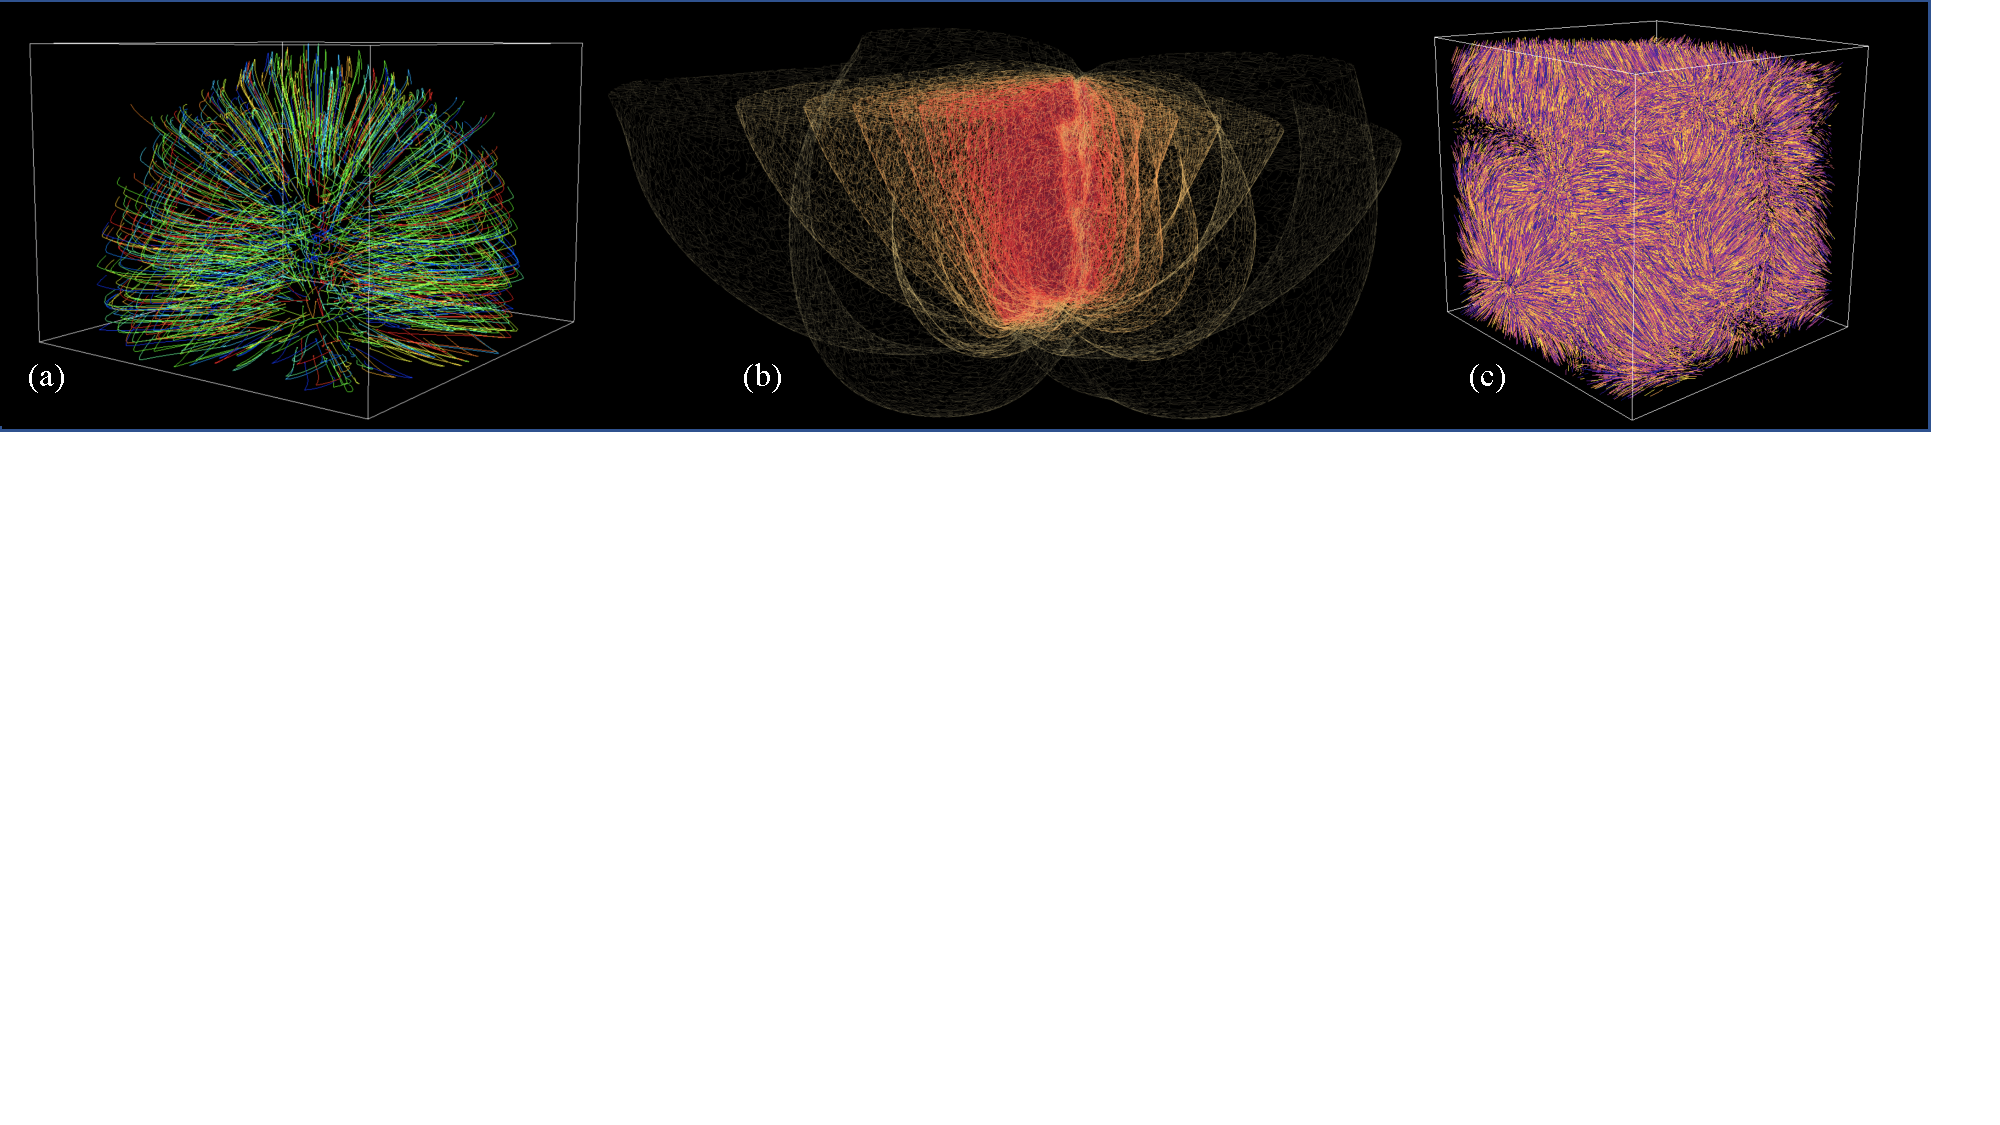
\includegraphics[width=\linewidth, trim={0cm 11.5cm 2cm 0cm}, clip]{images/Teaser_Vis.pdf}
  \label{fig:teaser}
	\caption{Visualizations of the simulation codes we demonstrate vector field data reduction for using a Lagrangian representation. L-R: (a) Cloverleaf3D pathlines depicting initial behavior in domain; (b) SW4 displacement magnitude derived from basis trajectories computed over 1000 cycles capturing seismic wave propagation using contour lines; (c) Nyx pathlines for 25 cycles of simulation. }
}

%% Uncomment below to disable the manuscript note
%\renewcommand{\manuscriptnotetxt}{}

%% Copyright space is enabled by default as required by guidelines.
%% It is disabled by the 'review' option or via the following command:
% \nocopyrightspace


\vgtcinsertpkg

%%%%%%%%%%%%%%%%%%%%%%%%%%%%%%%%%%%%%%%%%%%%%%%%%%%%%%%%%%%%%%%%
%%%%%%%%%%%%%%%%%%%%%% START OF THE PAPER %%%%%%%%%%%%%%%%%%%%%%
%%%%%%%%%%%%%%%%%%%%%%%%%%%%%%%%%%%%%%%%%%%%%%%%%%%%%%%%%%%%%%%%%

\begin{document}

\setlist{nolistsep}

%% The ``\maketitle'' command must be the first command after the
%% ``\begin{document}'' command. It prepares and prints the title block.

%% the only exception to this rule is the \firstsection command
%\firstsection{Introduction}

\maketitle
\section{Introduction}
\label{sec:introduction}
%The notion of calculating particle trajectories for a scientific simulation ``online'' for ``offline'' exploration was first explored by Vries et al.~\cite{vries2001calculating} in the context of ocean circulation models.
%
More recently, motivated by the large data analysis and visualization~(DAV) challenges on modern supercomputers, Agranovsky et al.~\cite{agranovsky2014improved} conceptually explored the use of a reduced Lagrangian representation of a time-dependent vector field.
%
The proposed data reduction technique would operate in situ~(``online'') alongside the simulation and calculate particle trajectories using the complete spatial and temporal resolution of the simulation.
%
The reduced data could then be reconstructed post hoc~(i.e., ``offline'') to support the exploration DAV use case.
%
Although the findings showed improved post hoc~(i.e., ``offline'') exploration capabilities (greater integrity and reduced data size), it was demonstrated in a theoretical in situ setting, i.e., data set files were loaded from disk to mimic a simulation.
%
Several research studies following the work by Agranovsky et al.~\cite{agranovsky2014improved} have furthered the state of the art in terms of adoption~\cite{envirvis.20171099,siegfried2019tropical}, error analysis~\cite{bujack2015lagrangian, hummel2016error, chandler2016analysis}, accuracy-storage propositions~\cite{sane2018revisiting}, sampling strategies~\cite{rapp2019void, sane2019interpolation}, search structures and interpolation techniques~\cite{chandler2015interpolation, sane2019interpolation}. 
%
However, none of these works have provided a focused study of the cost and technical performance characteristics of calculating a Lagrangian representation of a time-dependent vector field on a supercomputer and integrated with a simulation as an in situ data reduction operator.
%
In this paper, we present an empirical study of the in situ encumbrance and performance tradeoffs when executing \textit{in situ Lagrangian analysis} in a practical setting, i.e., in situ on a supercomputer.

In situ Lagrangian analysis utilizes access to the complete spatial and temporal resolution of the simulation vector field to accurately calculate sets of particle trajectories, i.e., a Lagrangian representation of the vector field. 
%
However, this requires performing a particle advection step for every particle every cycle.
%
Assuming a tightly coupled in situ integration, i.e., simulation code and DAV routines share the same resources, the in situ encumbrance would depend on the number of particles and the parallelization hardware.
%
Unlike most particle advection studies, operating in situ requires returning control of compute resources to the simulation after every step.
%
Further, varying the number of particles used affects the integrity of the reconstruction.
%
Using a greater number of particles to sample the domain costs more in storage, runtime memory, and execution time, but provides high reconstruction integrity.
%
On the other hand, using less particles costs less in storage, runtime memory, and execution time, but provides worse reconstruction integrity. 
%
Assessing the in situ encumbrance introduced by varying workloads is critical to understand the viability of calculating a Lagrangian representation of a large time-dependent simulation vector field.
%

Our contributions in this paper are:
\begin{itemize}
\item An empirical study to evaluate the cost and understand the technical performance characteristics of in situ Lagrangian analysis on a modern supercomputer.
\item A quantitative analysis of reconstruction integrity using multiple metrics and histograms.
\item A qualitative analysis of reconstruction integrity using pathline visualizations.
\item Preliminary costs of implementing a Lagrangian-based advection scheme for distributed-memory post hoc reconstruction.
\end{itemize}






%
%would generate particle trajectories by accessing the complete spatial and temporal resolution on the simulation
%
%
%However, this initial work (to the best of our knowledge) was almost two decades ago.
%%
%This concept has received increased interest in recent years, specifically, with respect to the use of a Lagrangian representation of a vector field
%%
%Exploratory and accurate time-dependent vector field data analysis and visualization 
%
%historically been a challenging task.
%
%
%
%This resurgence is largely attributed
%
%
%
%%
%Large scientific simulation codes produces large amounts of data, not all of which can reasonably be stored to disk.
%%
%The lack of access to the complete spatial and temporal resolution of the simulation data has reduced the integrity of the data analysis and visualization of time-dependent vector fields.
%%
%In the past decade, several data analysis and visualization pipelines have had to react to the increasing gap between compute capability, i.e., our ability to generate large amounts of data, and our I/O capability, i.e., our ability to read, write and store data.
%%
%Operating on simulation data as it is generated, or \textit{in situ processing}, is an emerging paradigm has helps address this issue in one of two ways: 1) generate visualizations as the simulation generates data, or 2) process and reduce data for later exploration.
%%
%The first way is most useful when the desired data analysis and visualization is known a priori.
%%
%However, this approach is less useful for the exploratory use case, i.e., when there is no a priori knowledge about desired visualizations.
%%
%In this situation, i.e., the exploratory use case, storing a reduced data set appears to be viable path forward.
%
%
%In situ Lagrangian analysis is one of few uniquely positions operators that performs data reduction of a vector field by operating on it every cycle. 
%%
%This also raises questions around the cost of in situ Lagrangian analysis. 
%%
%Performing particle advection for a 1000 steps is very different from performing particle advection for a 1000 steps, but giving up control of the hardware accelerators after each step.
%%
%It is important to understand the costs of these operations in settings involving a simulation. 
%%
%We do this in this empirical study.
%
%Exploratory analysis and visualization of time-dependent vector fields using traditional methods is increasingly challenging on modern supercomputers.
%%
%Modern supercomputing trends clearly show an increasing gap between computational and I/O capabilties, i.e., we can compute and generate far more data than we can reasonably save to disk.
%%
%The massive increase in compute power has enabled scientists to model phenomena of interest in far greater detail than we could previously.
%%
%The limited increase in I/O capabilities, however, increases the pressure on the data analysis and visualization pipeline.
%%
%To address the I/O bottleneck, scientists frequently resort to temporal subsampling, i.e., store data to disk less frequently or at select cycles.
%%
%To perform accurate exploratory data analysis and visualization, particularly of time-dependent data, requires access to the data, both spatial and temporal.
%%
%As the I/O gap continues to grow, sparse temporal subsampling using traditional methods will fail to maintain high integrity during time-dependent vector field analysis and visualization.
%
%
%In situ processing has gained popularity in recent years as a potential solution to address the I/O bottleneck.
%%
%The in situ processing paradigm enables operations to be performed on the data \textit{in place}, i.e., in memory, and provides access to the complete spatial and temporal resolution of the simulation data.
%%
%Routines that operate in situ typically adopt one of two strategies: perform analysis and visualization routines directly or perform data reduction to enable post hoc exploratory analysis and visualization.
%%
%Both strategies aim to alleviate the burden on the I/O bandwidth.
%%
%In this paper, we will focus on an in situ data reduction routine for time-dependent vector field data. 
%%
%Time-dependent vector field data is transformed by calculating a reduced Lagrangian representation of the field and stored to disk.
%%
%The opportunity of in situ processing, however, comes at the cost of an encumbrance on the simulation code.
%%
%For an in situ method to be viable, it is critical this method operate within in situ constraints and remain within an allocated resource budget.
%%
%Failing to operate within constraints would adversely impact the performance of the simulation code, which could lead to further undesirable consequences. 
%%
%Thus, it is critical to understand the technical performance characteristics of an in situ routine in a practical setting, i.e., at scale on a modern supercomputer.
%
%The high cost of operating a modern supercomputer makes time on compute nodes a valuable resource.
%%
%Scientists will typically identify a percentage of time and memory that can be allocated for in situ data analysis and visualization routines.
%%
%Further, scientists can specify the frequency at which routines can perform computation and/or store data to disk, i.e., every cycle or every $X^{th}$ cycle ($X > 1$).
%%
%In situ data reduction by calculating a Lagrangian representation of the time-dependent vector field, or \textit{in situ Lagrangian analysis}, requires access to the simulation data every cycle and involves the computation of particle trajectories that track the displacement of a particle over time.
%%
%These operations require performing operations associated with particle advection and storing of particle information in memory. 
%%
%Our study evaluates the in situ cost by deploying this data reduction operator in a practical setting on a supercomputer. 
%
%Although multiple works have studied various aspects of using a Lagrangian representation, such as storage-accuracy propositions, error analysis, and interpolation, the practical cost of deploying this technique in a large-scale distributed environment and its impact on a simulation code has not been considered.
%%
%We present a 
%
%The concept of representing time-dependent vector field data using a Lagrangian representation was first explored for ocean and atmosphere general circulation models~\cite{}.
%%
%This technique was more recently applied as a data reduction operator by Agranovsky et al.~\cite{agranovsky2014improved}.
%%
%The study by Agranovsky et al. demonstrated significantly improved data storage-accuracy propositions could be achieved using this method.
%%
%Further, visual analysis of ocean model simulations using reduced Lagrangian representations of time-dependent vector field data demonstrate early adoption of this approach.
%%
%
%
% been explored 


Flow visualization is an important sub-area of scientific visualization for
understanding vector field data.
%
Most flow visualization techniques involve placing massless particles at seed positions
and displacing them according to the vector field,
whether for animating particles, plotting the entire trajectory at once (streamlines/pathlines),
or using particle trajectories as building blocks for other techniques (e.g., finite-time Lyapunov exponents).
%
Most often, the movements of particles are calculated by solving an ordinary differential equation, typically
with a Runge-Kutta algorithm~\cite{cash1990variable}.
%
%The accuracy of this solution is well studied and has been generally deemed as acceptable for
%flow visualization techniques.
%
%That said, 
Algorithms like Runge-Kutta require evaluating the velocity field at multiple locations;
the popular fourth order algorithm (RK4) requires evaluation at four locations.
%
When dealing with steady-state flow, the velocity field evaluations can be performed accurately,
with error typically only arising from interpolation within a cell of a mesh.
%
However, when dealing with unsteady-state flow, accurate velocity field evaluations can be 
%much more difficult 
harder to achieve.

The primary problem with accurate velocity field evaluation for unsteady-state flow 
is that computational simulations are unable to store full spatio-temporal data.
%
These simulations often advance in ``cycles.''
%
During a cycle, the simulation advances from its current time, $T$, to a new time, $T+\epsilon$.
%
%The simulation does this by solving equations and applying their solutions to update the values of fields on its mesh.
%
Simulations run for many cycles, from thousands to hundreds of thousands.
%
%Simulations run for thousands to hundreds of thousands of cycles.
%
Saving simulation state to disk often is very costly, both in the time to interact with the I/O system and in
storage costs (bytes).
%
%Further, the values of the fields often change by only small amounts from one cycle to the next.
%
In response, simulations almost uniformly practice ``temporal subsampling,''
meaning that they save data from only a subset of their cycles to disk.
%
%\fix{New sentence from Hank:}
With respect to unsteady-state flow, this means that velocity field evaluation must
do temporal interpolation; further, as fewer and fewer cycles are stored, these interpolations
are increasingly inaccurate, introducing increasing error into flow visualizations.

%The methods for temporal subsampling vary, but common practices include saving one out of every $N$
%cycles or saving after some amount of time elapses.

With this work, we consider a class of flow visualization problems with three properties:
\begin{tightEnumerate}
\item The flow visualization is exploratory, i.e., the desired particle trajectories will 
be specified by a domain scientist during an interactive visualization session after the simulation completes.  
As a result, the desired particle trajectories are not known while the simulation is running.
\item The flow visualization needs to consider unsteady-state flow (the vector field data from one cycle will not suffice).
\item The simulation is saving data to disk at a low rate, i.e., sparse temporal subsampling.
\end{tightEnumerate}
%
We refer to this as an \textbf{EUS} problem: 
\textbf{E}xploratory analysis
+ 
\textbf{U}nsteady-state flow 
+ 
\textbf{S}parse temporal subsampling.
%
We note that removing any of these three properties simplifies the problem substantially:
\textbf{US} can calculate particle trajectories \textit{in situ} while the simulation is running,
\textbf{ES} does not require inferring velocity field values between cycles, 
and
\textbf{EU} can infer velocities between time slices (reasonably) accurately.

\textbf{EUS} problems have occurred more often on supercomputers in recent years.
%
Over the last decade, the ability to generate data on supercomputers has gone up by $\sim$100X, 
but I/O capabilities have gone up by $\sim$10X.
%ability to store and load data on supercomputers has gone up by only $\sim$10X.
%
As a result, simulations must the reduce proportion of the data they store, 
often creating \textbf{S}parse temporal sampling.
%
Additionally, 
while supercomputers are a major motivator for considering \textbf{EUS} problems,
these problems also are important in non-supercomputing environments.

\textit{In situ} processing~\cite{ma2009situ, bauer2016situ}
is an important approach for addressing the ``I/O bottleneck.''
%
Most typically, 
\textit{in situ} processing utilizes 
\textit{a priori} knowledge of which visualizations and analyses to complete.
%
However, 
this \textit{in situ} style is not congruent with the \textbf{E}xploratory component of \textbf{EUS} problems.
%
Fortunately, an alternate worklow avoids the need for \textit{a priori} knowledge,
by using 
a combination of \textit{in situ} and \textit{post hoc} processing~\cite{JSFI78}.
%
In the \textit{in situ} phase, 
data is transformed and reduced so that it is small enough to be saved to
disk.
%
In the \textit{post hoc} phase, this data is used to perform
exploratory visualization.
%
In the context of flow visualization, this means that \textit{in situ} processing should transform
and reduce time-varying vector field data such that \textit{post hoc} exploration can use the result to
infer arbitrary particle trajectories ---
ideally with high accuracy and requiring little data storage, among
other properties.

An important consideration with this \textit{in situ} + \textit{post hoc} workflow is how to transform and reduce data.
%
For our work, we transform/reduce spatio-temporal vector data using a Lagrangian 
approach.
%
This choice enables data from all cycles of a simulation to be represented,
which is fundamentally different than the traditional choice of saving time slices.
%
We refer to this Lagrangian-based workflow as \textbf{L-ISR-PHE}: \textbf{L}agrangian-based \textbf{I}n \textbf{S}itu \textbf{R}eduction with
\textbf{P}ost \textbf{H}oc \textbf{E}xploration.

Agranovsky et al.~\cite{agranovsky2014improved} performed the seminal study on applying 
\textbf{L-ISR-PHE} to the \textbf{EUS} problem, but their study left significant questions.
%
In particular, while their work demonstrated promising accuracy-storage tradeoffs,
their work failed to seriously consider whether the approach could be practically deployed.
%
Further, follow-on studies have also not considered practical deployment, instead focusing
on better understanding accuracy-storage tradeoffs or improving \textit{post hoc} interpolation.
%
As a result, a significant open question is whether the \textbf{L-ISR-PHE} approach is practical.
%
The open nature of this question has hindered both follow-on research and widespread adoption.
%
%Our study addresses this gap.


The contribution of this paper is an empirical study on 
the \textbf{L-ISR-PHE} workflow to the \textbf{EUS} problem.
%
It considers \textbf{L-ISR-PHE} holistically: considering evaluation criteria at each phase of processing,
defining metrics to measure these criteria, defining workloads of interest, and then evaluating
the workloads and metrics in a large study.
%
One highlight of our study is that it is the first
to evaluate the encumbrance placed on a simulation code during \textit{in situ} reduction.
%
Of note, all previous studies ran in ``theoretical'' in situ environments, meaning that
they loaded data sets from disk, rather than truly integrated with a simulation code.
%
Another highlight is that our study provides detailed quantitative evaluations of the extracted 
Lagrangian data, as well as an estimate of costs for distributed 
memory \textit{post hoc} reconstruction.
%
Previous studies have failed to consider the distribution of outcomes when inferring new particle trajectories,
instead focusing on average behavior.
%
In all, our empirical study provides
the most clear evidence to date that \textbf{L-ISR-PHE} is viable and 
should be the preferred solution for most \textbf{EUS} problems.
%
%Our study considers  three diverse simulation codes running on a top supercomputer, with experiments calculating over 76M particle trajectories using up to $384$ GPUs.
%


%Paragraph 2: LB-ISE-PHE is a solution to the E-TVVD-STS problem.
%
%Paragraph 3: Although some preliminary studies have shown the promise
%of LB-ISE-PHE for the E-TVVD-STS problem in a theoretical in situ
%environment, a major motivation for the technique is in a large-scale
%supercomputing environment with actual in situ runs.
%%
%This has never been done, but is critical to establishing the viability
%of the LB-ISE-PHE solution to the E-TVVD-STS problem.  And we do that here.
%
%important issues remain open 
%(e.g., in situ emcumbrance, actually done real world in situ).
%
%With this work, we perform an empirical study of the LB-ISE-PHE approach
%to the E-TVVD-STS problem.
%
%We consider issues in depth that have been ignored in previous works, specifically
 %in situ encumbrance, etc.
%

%Paragraph 4:
%The result of this study is to demonstrate that stakeholders with the E-TVVD-STS
%problem should be employing the LB-ISE-PHE in almost all cases.
%
%How does it differ going from a theoretical in situ environment to a real-world
%in situ environment?:
%- can measure percentage of run-time (which involves both particle advection
%time and simulation cycle time)
%- the invocation (not best word) of particle advection differs when constrained
%to operate in situ
%- real world I/O output
%- memory concerns
%- data generated is large, and requires parallel post hoc
%
%If you have problem E-TVVD-STS, then you want solution LB-ISE-PHE.
%
%Then the Lagrangian-based in situ extraction + post hoc exploration is for you!
%
%
%
%in situ Lagrangian analysis
%time-varying vector data
%post hoc exploration
%
%With this study, we contribute an empirical study of 


\section{Background and Related Work}
\label{sec:related}
\setlength{\belowdisplayskip}{0pt} \setlength{\belowdisplayshortskip}{0pt}
\setlength{\abovedisplayskip}{0pt} \setlength{\abovedisplayshortskip}{0pt}

\subsection{Frames of Reference}
%
In fluid dynamics, there are two frames of reference to observe fluid motion: Eulerian and Lagrangian.
%
With the Eulerian frame of reference, the observer is in a fixed position.
%
With the Lagrangian frame of reference, the observer is attached to a fluid parcel and is moving through space and time.

%
When a flow field is stored in an Eulerian representation, it is typically done by means of its velocity field.
%
A velocity field $v$ is a time-dependent vector field that maps each point $x\in \mathbb R^d$ in space to the velocity of the flow field for a given time $t\in \mathbb R$
%
\begin{eqnarray}
{v} : \mathbb R^d \times \mathbb R \to \mathbb R^d,\; x,t \mapsto v(x,t)
\end{eqnarray}

%In a practical setting, the vector field is defined over a fixed, discrete mesh and represents the state of the flow field at a specific instant of time or time slice, i.e., at a specific simulation time and cycle.
%
In a practical setting, a flow field at a specific time/cycle is defined as a vector data on a fixed, discrete mesh.
%
Time-varying flow is represented as a collection of such data over a variety times/cycles.


When a flow field is stored in a Lagrangian representation, it is done by means of its flow map $F_{t_0}^{t}$.
%
The flow map is comprised of the starting positions of massless particles $x_0$ at time $t_0$ and their respective trajectories that are interpolated using the time-dependent vector field.

Mathematically, a flow map is defined as the mapping
\begin{eqnarray}
F_{t_0}^{t}(x_0):\mathbb R \times \mathbb R \times \mathbb R^d \to \mathbb R^d,\; t \times t_0 \times x_0 \mapsto F_{t_0}^{t}(x_0) = x(t)
\end{eqnarray}
%
of initial values $x_0$ to the solutions of the ordinary differential equation
%
\begin{eqnarray}
\frac{d}{dt}x(t) = v(x(t),t)
\end{eqnarray}

In a practical setting, the flow map is represented as sets of particle trajectories calculated in the time interval $[t_0,t]\subset \mathbb R$.
%
The stored information, encoded in the form of known particle trajectories (i.e., a Lagrangian representation), encodes the behavior of the time-dependent vector field over an interval of time.
%

Although the frames of reference are theoretically equivalent~\cite{bujack2015lagrangian}, their application in practical settings varies. 
%
Our interest with this study is the practical setting, specifically for the \textbf{EUS} problem.
%


\subsection{In Situ Reduction via Lagrangian Representations}
As referenced in the introduction, Agranovsky et al.~\cite{agranovsky2014improved}
presented the first work on applying \textbf{L-ISR-PHE} to \textbf{EUS}.
%
Their work compared to a traditional Eulerian approach, i.e., saving cycles at regular
intervals and calculating pathlines using temporal interpolation.
%
Their findings demonstrated significant benefits, for example 12X improvements in accuracy
using the same storage, as well as the same accuracy for 64X less storage.
%
The key intuition behind these results is that the Lagrangian representation captures the
 behavior of the flow field over an interval of time, as opposed to the state at a single time slice, and 
thus is able to store more information per byte with respect to \textbf{EUS}.
%
%Despite highlighting the promise of \textbf{L-ISR-PHE}, the Agranovksy et al. work also had shortcomings.
%
%As already mentioned, one shortcoming was a lack of evaluation on \textit{in situ} encumbrance, 
%which was not possible since they did not perform \textit{in situ} experiments.
%
%Another shortcoming was in evaluation, as their metrics only showed results relative to the traditional
%Eulerian approach, creating uncertainty about whether or not the absolute errors were significant.
%
%Finally, their strategy for placing particles was to use uniform placement, terminated at uniform intervals.
%

Subsequent research studies have broadened the understanding and exploration of the \textbf{L-ISR-PHE} paradigm.
%
Sane et al.~\cite{sane2018revisiting} evaluated the \textbf{L-ISR-PHE} workflow for a range of spatiotemporal configurations operating on a fixed storage budget and provided absolute error estimates. 
%
Most recent research has explored sampling strategies for particle trajectories that form the Lagrangian representation.
%
Sane et al.~\cite{sane2019interpolation} explored the use of longer trajectories and 
%a Delaunay triangulation-based method to 1) identify candidate locations to introduce new particles, or 2) terminate existing trajectories.
%
%Additionally, they
proposed an interpolation scheme to reduce error by evaluating neighborhoods across interpolations.
%
Rapp et al.~\cite{rapp2019void} applied their void-and-cluster sampling technique to identify a representative set of scattered particles and found that it performs better than random sampling. 
%
To address scalability challenges, Sane et al.~\cite{sane2020scalable} explored an accuracy-performance tradeoff and demonstrated the use of a communication-free model that only stored trajectories that remain within the rank domain during the interval of computation.
%

%Although these studies have advanced the state of the art, none of these works inform the cost of \textbf{L-ISR-PHE} on a modern supercomputer.
%
%Assuming a tightly coupled in situ integration, the simulation code and in situ routine swap control of compute resources every cycle to compute a Lagrangian representation.
%
%This requires performing a single particle advection step for every particle every cycle.
%
%Critically, this is unlike previous particle advection studies that load particles into memory once and perform thousands of steps.
%
%The in situ phase utilizes access to the complete spatial and temporal resolution of the simulation vector field to accurately calculate sets of particle trajectories, i.e., a Lagrangian representation of the vector field.
%
%
%Further, the in situ encumbrance is closely related to the number of particles (directly impacts storage and integrity) and the parallelization hardware.
%
%Unlike most particle advection studies, operating in situ requires returning control of compute resources to the simulation after every step.
%
%Further, varying the number of particles used affects the integrity of the reconstruction.
%
%Using a greater number of particles to sample the domain costs more in storage, runtime memory, and execution time, but provides high reconstruction integrity.
%
%On the other hand, using less particles costs less in storage, runtime memory, and execution time, but provides worse reconstruction integrity.
%
%Assessing the in situ encumbrance introduced by varying workloads is critical to understand the viability of calculating a Lagrangian representation for a large time-dependent simulation vector field.
%
%\fix{So all we are doing is evaluating in situ encumbrance?}

%\fix{In Section~\ref{sec:isr_evaluation_criteria}, we propose evaluation criteria for \textit{in situ}
%encumbrance.
%While these prior works have informed critical components of the \textbf{L-ISR-PHE} workflow,
%we feel none significantly inform these evaluation criteria, which has been a critical barrier to adoption.}


\subsection{Lagrangian Extract-Based Post Hoc Exploration}
The notion of calculating particle trajectories for a scientific simulation ``online'' for ``offline'' exploration was first explored by Vries et al.~\cite{vries2001calculating} in the context of ocean circulation models.
%
Next, Hlawatsch et al.~\cite{hlawatsch2011hierarchical} proposed a pathline interpolation technique that employs a hierarchical scheme and assumes access to the data across multiple time steps.
%
The technique constructs longer, more accurate trajectories by decreasing the number of integration steps when using previously computed particle trajectories.
%
Chandler et al.~\cite{chandler2015interpolation} proposed a modified k-d tree as a search structure and an interpolation technique for Lagrangian data extracted from an SPH simulation.
%
Further, Chandler et al.~\cite{chandler2016analysis} conducted error analysis studies and identified correlations between Lagrangian-based interpolation error and divergence in the flow field.
%
Bujack et al.~\cite{bujack2015lagrangian} evaluated the use of parameter curves to fit interpolated pathline points to improve the aesthetic of trajectories calculated using Lagrangian data.
%
Hummel et al.~\cite{hummel2016error} provided theoretical error bounds for error propagation and accumulation that can occur when calculating pathlines using Lagrangian data. 
%
With respect to adoption of ~\textbf{L-ISR-PHE}, 
Agranovsky et al.~\cite{agranovsky2014improved}'s introduced a scheme, although their interpolation
was straightforward since their \textit{in situ} scheme place particles at uniform locations
and terminating them at regular intervals.
Recently, Pascal et al.~\cite{envirvis.20171099,siegfried2019tropical} used extracted Lagrangian data from an ocean modeling simulation to explore coastal upwelling activity and visualize a derived scalar field representing pathline density.

%\fix{In Section~\ref{sec:phe_evaluation_criteria}, we propose evaluation criteria for \textit{post hoc}.
%While previous studies have answered questions about inferring new pathlines from existing pathlines,
%only the Agranovsky et al. work considered accuracy from the \textbf{L-ISR-PHE} workflow.  
%A key differentiator for our empirical study is that we consider real supercomputing applications
%at scale, as opposed to the previous study which included analytical data and desktop-level simulations.
%As a result, we feel our findings will be more persuasive to the broader community about the efficacy
%of \textbf{L-ISR-PHE}.}



\subsection{Other Relevant Research}
Within the vector field analysis and visualization community, Lagrangian methods have been increasingly used in the past decade.
%
Lagrangian coherent structures (LCS) are a popular technique to visualize attracting and repelling surfaces and were introduced by Haller et al~\cite{haller2001distinguished, haller2000lagrangian, haller2000finding}.
%
The interest in the technique led to multiple efforts that were aimed at accelerating the computation and visualization of LCS~\cite{garth2007efficient,garth2009visualization,sadlo2007efficient,sadlo2011time}.
%
LCS have also been used for uncertain transient vector field visualization by Guo et al.~\cite{guo2016finite}.
%

Finally, multiple works have proposed vector field reduction strategies while maintaining an Eulerian representation.
%
Lodha et al.~\cite{lodha2000topology} controlled the compression of similar vectors into single vectors representing larger area.
%
Further, Lodha et al.~\cite{lodha2003topology} proposed a top-down topology preserving compression technique.
%
Theisel et al.~\cite{theisel2003combining} computed critical points and viewed the task as a mesh reduction, and later provided a threshold to filter important features~\cite{theisel2003compression}.
%
Each of these studies performed compression on the vector field of a single time step.
%
With the objective of highlighting temporal features of the vector field, Tong et al.~\cite{tong2012salient} compressed the total amount of data steps stored by identifying key time steps.
%
Although these techniques could be used to reduce data and store more frequently, these approaches don't inherently address the challenge of increasing temporal sparsity.
%Although these techniques are valuable, they do not sufficiently address the challenge of increasing temporal sparsity.
%
%\fix{I think we need a better statement here --- could reduce to get higher temporal sparsity.  And yet don't want to compare with that.}
%For a baseline comparison in our empirical study, we store data in an Eulerian representation at full resolution and use temporal subsampling.



%This paper presents an empirical study of the in situ encumbrance and performance tradeoffs when executing \textit{in situ Lagrangian analysis} in a practical setting, i.e., in situ on a supercomputer.



\section{Evaluating L-ISR-PHE}
%\section{Lagrangian-Based In Situ Reduction with Post Hoc Exploration}
\label{sec:methodology}
\begin{figure}
\centering
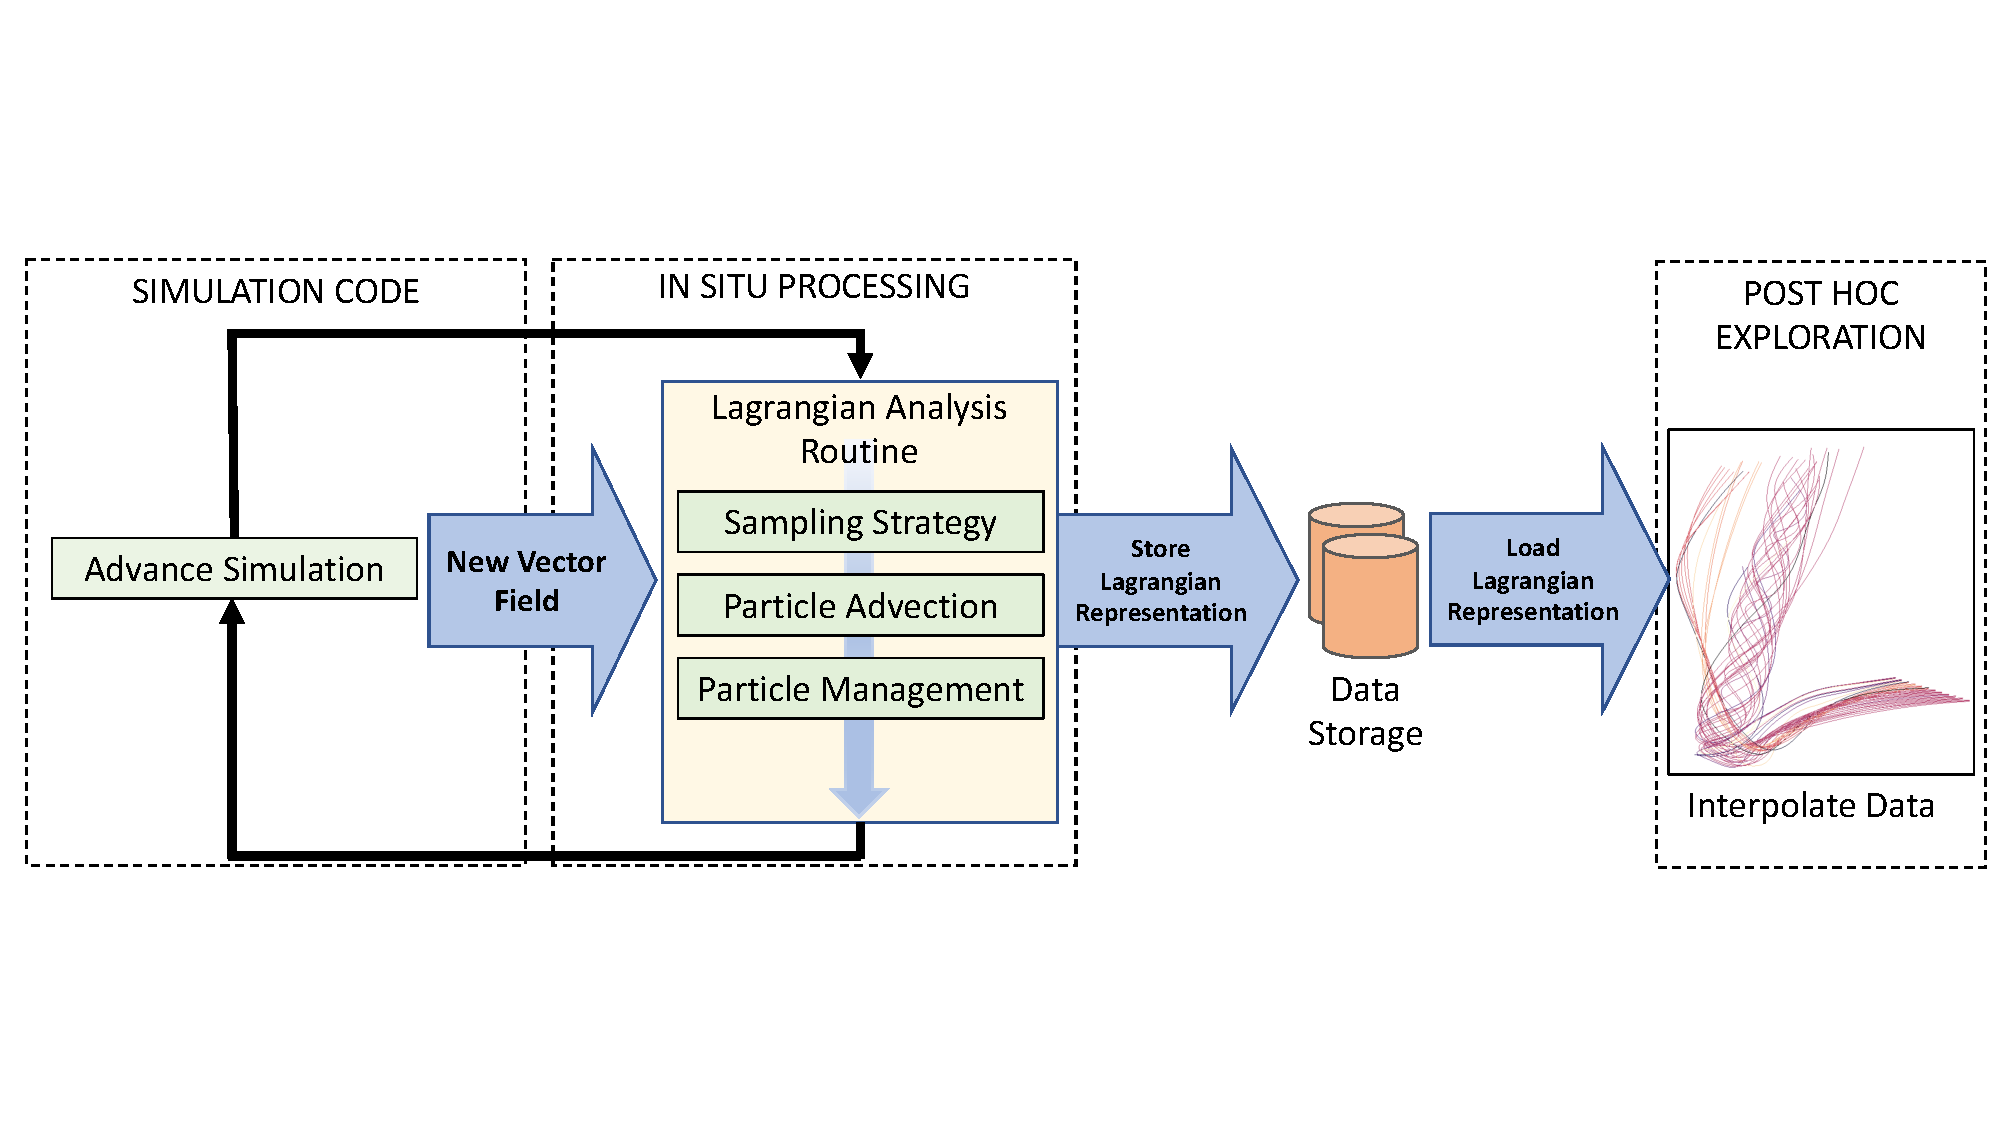
\includegraphics[width=\linewidth,trim={0cm 4.3cm 0cm 4.3cm}, clip ]{images/Schematic.pdf}
\vspace{-6mm}
\caption{Schematic diagram of the \textbf{L-ISR-PHE} workflow showing \textit{in situ} processing, data storage, and \textit{post hoc} exploration.}
\label{fig:schematic}
\vspace{-6mm}
\end{figure}

This section describes considerations for an empirical study of the \textbf{L-ISR-PHE} workflow.
%
Specifically: 
\begin{tightItemize}
\item Subsection~\ref{sec:instantiation} describes the instantiation we consider. 
\item Subsection~\ref{sec:eval} describes evaluation criteria.
\item Subsection~\ref{sec:workloads} describes important factors in defining workloads.
\end{tightItemize}

%This section describes our specific choice of instantiation for each of the components of the \textbf{L-ISR-PHE} workflow, i.e., in \textit{situ reduction}, data storage, and \textit{post hoc} exploration. 
%%
%
%Our discussion includes, when applicable, identifying ``areas'' to evaluate the components.
%
%We encode these in parentheses and name them based on the component they relate to.
%
%Next, in Section~\ref{sec:parameters} we discuss the parameter space we explore and identify which ``areas'' of the \textbf{L-ISR-PHE} workflow it impacts. 




%In this section, we first identify the evaluation areas for the in situ reduction, data storage, and post hoc exploration components of the \textbf{L-ISR-PHE} workflow.
%%
%%
%Next, in Section~\ref{sec:instantiation} we specify our choice of instantiation for each of the components.
%
%\subsection{\textbf{L-ISR-PHE Workflow}}
%The \textbf{L-ISR-PHE} workflow has multiple components (schematic in Figure~\ref{fig:schematic}) that we discuss in the following subsections. 
%

\subsection{Instantiation}
\label{sec:instantiation}

Figure~\ref{fig:schematic} shows a high-level description of the
\textbf{L-ISR-PHE}  workflow.
%
There are many possible strategies for accomplishing the components
within this workflow, i.e., sampling strategy, particle management,
storage, and interpolation.
%
That said, we focus this empirical study on 
the current best practices in this space.
%

%This phase involves 
%At a high-level, extracting a Lagrangian representation involves a domain sampling strategy, performing advection every cycle of the simulation, and other particle management tasks (validating, storing, etc.).
%%
%Our empirical study adopts currently known best practice techniques to extract a Lagrangian representation at scale.
%
%For a domain sampling strategy, we adopt the

\textbf{\textit{In Situ} Reduction:}
\textit{In situ} reduction operates by maintaining a set of particles and their
trajectories.
%
As the simulation completes each cycle, it then invokes our visualization 
routines to update particle positions to reflect the advancement in time.
%
The main decisions for our visualization routines
 are when and where to introduce particles,
when to terminate particles, and what information to save about particles.
%
For this empirical study, we introduced particles using the 
uniform seed placement scheme from Agranovksy et al.~\cite{agranovsky2014improved}, including re-introducing particles at fixed intervals.
%
Our particle termination follows the 
communication-free model from Sane et al.~\cite{sane2020scalable}, where
particles are terminated either if they reach the end of the interval
of if they exit the block.
%
While this captures less information at the block boundaries, results show
that the overall loss of accuracy is very low, 
and the \textit{in situ} encumbrance is much reduced.
%
%The specific details of our implementation are in Section~\ref{sec:insituimp}.
%For each particle, we store only its final position, as its seed location
%can be represented implicitly.

\textbf{Data Storage:}
%
Lowering the encumbrance on file data storage systems is one of the primary motivators to use the \textbf{L-ISR-PHE} workflow.
%
Data storage costs can vary based on 1) how many particles are used to sample the domain, and 2) what information is stored for each particle.
%
Typically, when using more particles, and thus more data storage, a stakeholder would expect greater integrity during exploration.
%
Further, the efficacy of exploration can be closely tied to the nature of the stored data.
%
Although the general \textbf{L-ISR-PHE} framework can support complex Lagrangian reprensentations (unstructured particle sets, polynomial expressions, attribute information, etc.), these are yet unexplored. 
%
For our empirical study, a particle trajectory in the Lagrangian representation is stored using a start and end location of the trajectory during the interval of calculation, similar to previous works~\cite{agranovsky2014improved, sane2018revisiting, sane2020scalable}.
%
These saved particle trajectories are called ``basis flows.''
%

\textbf{\textit{Post Hoc} Exploration:}
The final phase of the \textbf{L-ISR-PHE} workflow involves 
exploratory flow visualization, which in turn requires
constructing new particle trajectories.
%
These new particles trajectories are constructed by 
interpolating from the basis flows.
%interpolating the information extracted to generate new time-dependent vector field visualizations.
%
As mentioned in the discussion of storage, 
the efficacy of the technique is dependent on the nature of the data stored.
%
Prior works have looked extensively at the theoretical and empirical error of Lagrangian-based advection schemes~\cite{hlawatsch2011hierarchical, bujack2015lagrangian, hummel2016error, chandler2016analysis, sane2018revisiting} and proposed methods to interpolate long trajectories~\cite{sane2019interpolation} and particles with non-zero mass~\cite{chandler2015interpolation}.
%
The essential operations involved in constructing new particle trajectories 
are identifying which basis flows to interpolate and performing interpolation.
%
Further,  
distributed-memory settings require communication to continue particle trajectory computation across node boundaries. 
%
Depending on whether the Lagrangian representation is structured or unstructured, different search structures are required.
%
We believe evaluating the cost of interpolating an unstructured particle set is more valuable, as it informs the general case.
%
Therefore, for our empirical study, 
we use the Lagrangian-based advection scheme described by Sane et al.~\cite{sane2020scalable}, to perform search structure~(Delaunay triangulation) construction in parallel and operate in a distributed-memory environment.
%
To perform interpolation on unstructured data, multiple scattered point interpolation schemes can be used.
%
However, the choice of interpolation scheme impacts efficacy, and thus, we use Barycentric coordinates, as recommended in a study by Agranovsky et al.~\cite{agranovsky2015subsampling}.


\subsection{Evaluation Criteria}
\label{sec:eval}

We consider evaluation criteria for each component of the workflow:
%\begin{tightItemize}
\textbf{\textit{In situ} reduction:}
\begin{tightItemize}
\item \textbf{ISR-1 Time:} the execution time spent by the simulation on data analysis and visualization. 
\item \textbf{ISR-2 Memory:} the runtime memory used by \textit{in situ} processing. 
\end{tightItemize}
\textbf{Data storage:}
\begin{tightItemize}
\item \textbf{DS-1 Size:} the file storage costs (i.e., bytes). 
\end{tightItemize}
\textbf{\textit{Post hoc} exploration:}
\begin{tightItemize}
\item \textbf{PHE-1 Time:} the execution time spent to construct new particle trajectories from basis flows
(search structure construction, interpolation, communication).
\item \textbf{PHE-2 Accuracy:} the accuracy of interpolated trajectories.
\end{tightItemize}
%\end{tightItemize}

\noindent
We also eliminated some criteria from consideration to limit scope:

\noindent
\textbf{\textit{In situ} reduction:}
We did not add an evaluation criteria to consider the ease of \textit{in situ}
integration.
%
This is an important concern, but we feel that it is beyond the scope
of this study. 
%
Further, there has been significant research on reducing the
burden on simulation codes to incorporate
\textit{in situ} visualization routines\cite{ayachit2016sensei,fogal2014freeprocessing,Larsen2017Ascent,liu2014hello,Vishwanath2011glean},
and so we are confident that this barrier will become
smaller over time.

\noindent
\textbf{Data storage:} We did consider and measure execution time, but found
supercomputing I/O times were very fast for our scale of study and often contained noise, likely due to contention on the supercomputer. 
%highly inconsistent due to contention,
%tension between latency and bandwidth, and other factors.  
More discussion can be found in~\ref{sec:iocost}.
%and other factors, and also performance varies
%based on latency and bandwidth.
%We did measure these as part of our study, and confirm the expected
%results: Lagrangian performance is always better than the traditional
%approach (since less data is being stored), and execution time goes
%down when less data is stored.  However, patterns beyond these broad trends
%are variable.
%We also considered file format challenges, but found that basis flows can be easily
%stored in existing formats.

\noindent
\textbf{\textit{Post hoc} exploration:} We did not consider if and whether Lagrangian-based extracts 
would affect specific flow visualization techniques.
%
For example, are techniques, such as path
surfaces or finite-time Lyapunov exponents, sensitive or insensitive
to the \textbf{L-ISR-PHE} workflow.  
We view this as future work.
%\end{tightItemize}

%
%\subsection{Evaluation Areas}
%\subsubsection{In Situ Reduction}
%\begin{itemize}
%\item \textbf{IS-E3 Ease of integration:} 
%\end{itemize}
%
%\subsubsection{Data Storage}
%\begin{itemize}
%\item \textbf{DS-E1 File size:}
%\item \textbf{DS-E2 File format:}
%\item \textbf{DS-E3 File write/read time:}
%\end{itemize}
%
%\subsubsection{Post Hoc Exploration}
%\begin{itemize}
%\item \textbf{PH-E1 Execution time:}
%\item \textbf{PH-E2 Accuracy:}
%\end{itemize}
%We identify that the in situ reduction phase can be evaluated along the axes of execution time~(\textbf{ISR-1}), memory~(\textbf{ISR-2}), and ease of integration~(\textbf{ISR-3}).
%
%Execution time and memory are critically important to evaluate the in situ encumbrance and we limit our study to these in this empirical study.
%

%Overall, to evaluate the post hoc phase of \textbf{L-ISR-PHE}, we identify the accuracy of interpolation~(\textbf{PHE-1}), and execution time~(\textbf{PHE-2}), i.e., the costs of performing reconstruction (search structure construction, interpolation, communication).

\subsection{Workload Factors}
\label{sec:workloads}
To understand the technique performance characteristics of the \textbf{L-ISR-PHE} workflow, we identified four parameters that when varied produce the workloads we want to evaluate for our empirical study. 
%Our approach to evaluate \textbf{L-ISR-PHE} involves exploring the technical performance characteristics across the parameter space shown in Table~\ref{}.
%Our study considers the following parameters:
\begin{itemize}
\item \textbf{Number of particles:} Our study varies the number of particles initialized per node and thus inform the cost of performing particle advection for varying workloads every cycle of the simulation. Further, the number of particles initialized is directly impacts the size of the data stored to disk and the accuracy of the reconstruction.
%
We specify the number of particles initialized using the notation \textbf{1:X}, where X is the reduction factor.
%
For example, a 1:1 configuration states that one particle is used for every grid point (no reduction) and a 1:8 configuration states that one particle is used for every 8 grid points (12.5\% of the original data size).
%

\textbf{Impacts $\rightarrow$} \textbf{ISR-1}, \textbf{ISR-2}, \textbf{DS-1}, \textbf{PHE-1}, \textbf{PHE-2}

\item \textbf{Interval:} We consider the interval or frequency at which files are stored to disk.
%
For a given total number of simulation cycles, this impacts the total amount of data stored to disk. 
%
Additionally, for the Lagrangian representation, the interval is equal to the integration length of each particle, and can thus, be consequential to the accuracy of reconstruction.
%
%For each configuration, we specify the number of cycles between storing to disk and refer to this as the \textbf{interval}.
%

\textbf{Impacts $\rightarrow$} \textbf{DS-1}, \textbf{PHE-1}, \textbf{PHE-2}

\item \textbf{Grid size:} We consider different grid sizes to measure the \textit{in situ} encumbrance of varying workloads.
%
Different grid sizes will use a different number of particles to sample the domain reasonably accurately.
%
In particular, we are interested in the \textit{in situ} encumbrance when a single compute node is operating on a large number of grid points.
%
An additional benefit of varying grid size is insight into the variation in simulation cycle time and consequently the percentage of time spent on \textit{in situ} processing.

\textbf{Impacts $\rightarrow$} \textbf{ISR-1}, \textbf{ISR-2}, \textbf{DS-1}

\item \textbf{Concurrency:} We consider the costs at various scale (i.e., number of compute nodes, MPI ranks). Further, the simulation codes required different parallelization hardware and thus, across simulation codes we measure the costs of Lagrangian representation extraction using, both, GPUs and CPUs for particle advection.

\textbf{Impacts $\rightarrow$} \textbf{ISR-1}, \textbf{PHE-2}
\end{itemize}



\section{Empirical Study Overview}
%\begin{figure*}[ht]
\centering
\begin{subfigure}{0.27\textwidth}
\centering
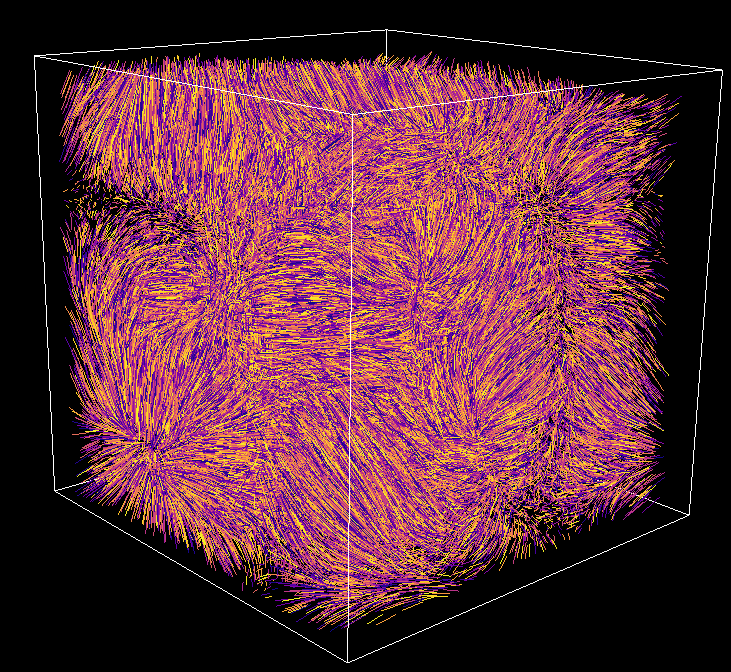
\includegraphics[height=4cm, keepaspectratio]{images/pathlines_nyx.png}
\caption{Nyx flow visualization}
\label{fig:pathlines_nyx}
\end{subfigure}
\hspace{-5mm}
\begin{subfigure}{0.32\textwidth}
\centering
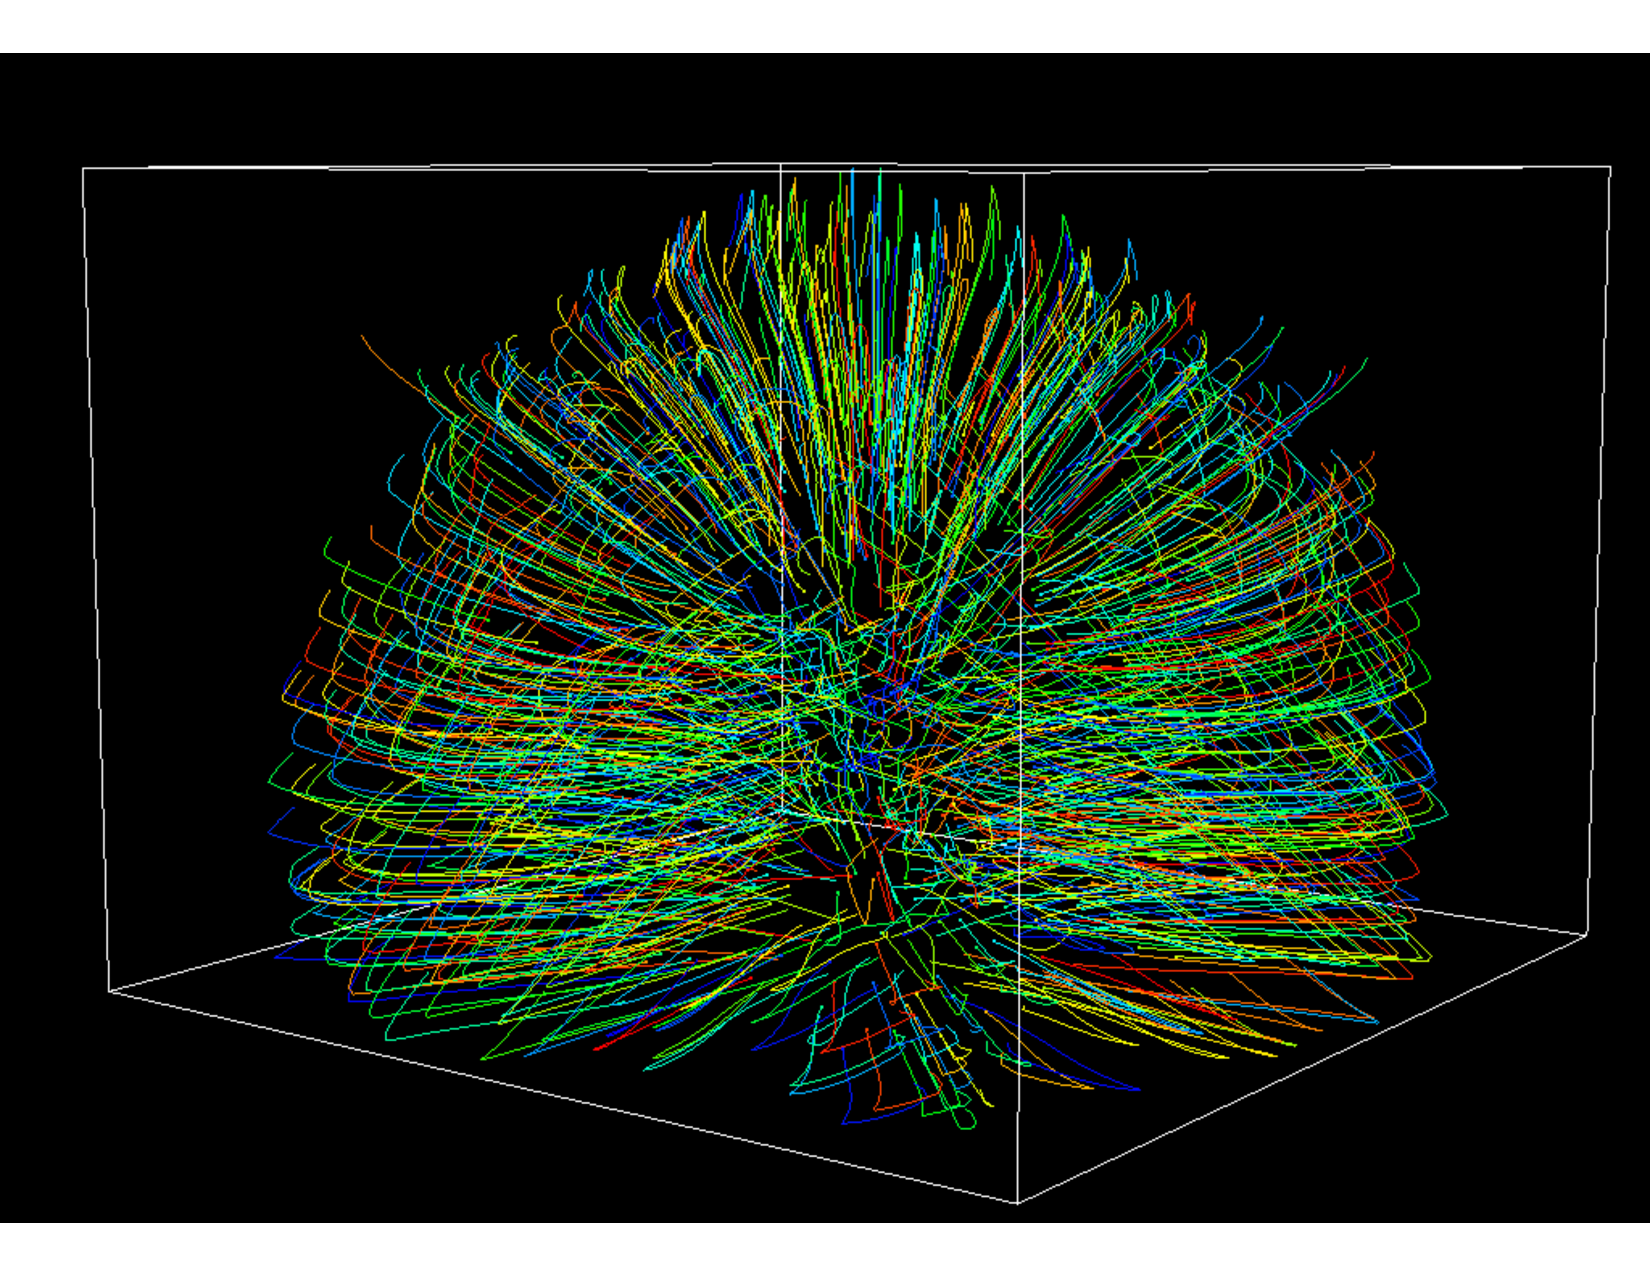
\includegraphics[height=4.36cm, keepaspectratio]{images/pathlines_clover.pdf}
\caption{Cloverleaf3D flow visualization}
\label{fig:pathlines_clover}
\end{subfigure}
\hspace{-5mm}
\begin{subfigure}{0.41\textwidth}
\centering
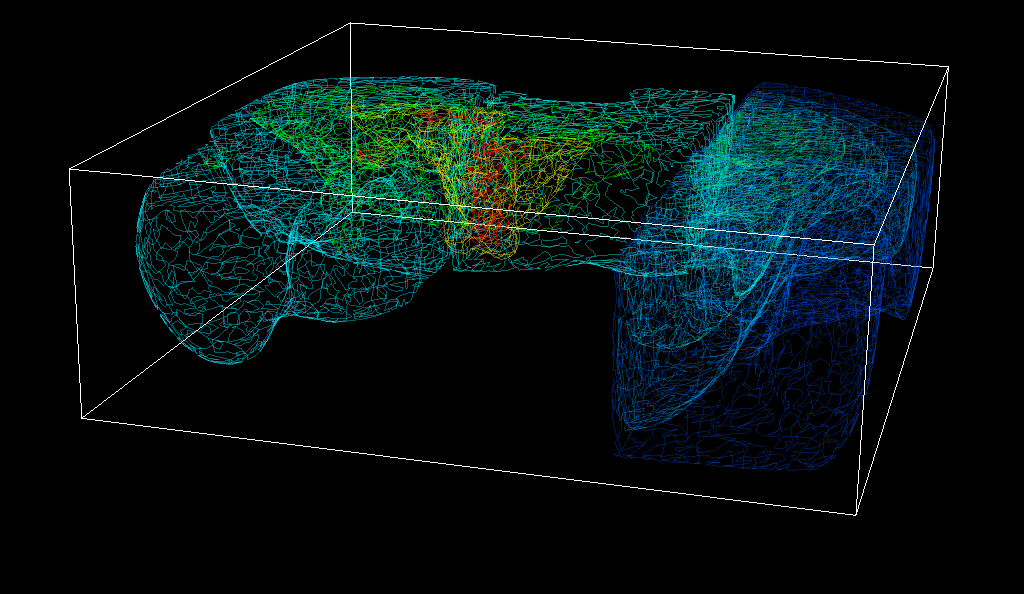
\includegraphics[height=4cm, keepaspectratio]{images/sw4_vis_2.png}
\caption{SW4 wave propagation visualization}
\label{fig:sw4_vis}
\end{subfigure}
\end{figure*}

%\begingroup
\setlength{\tabcolsep}{-2pt}
%\renewcommand{\arraystretch}{1} % Default value: 1
\begin{table*}[!h]
%\centering
\begin{tabular}{|P{1.1cm}|P{1.1cm}|P{2.7cm}|P{1.3cm}|P{1.3cm}|P{1.5cm}|P{2cm}  N  R|P{6cm}|}
\hline
Nodes & MPI & Dimensions & Interval & Sim$_{cycle}$ & Particles & Memory & Step & DAV\% & Scatter Plots\\ 
 & Ranks & & & & /Node & /Node (MB) & & & \\ 
\hline
%\multicolumn{9}{l}{} & \\
\multicolumn{9}{l}{\textbf{          Cloverleaf3D Proxy Hydrodynamics Application }} & \multirow{13}{*}{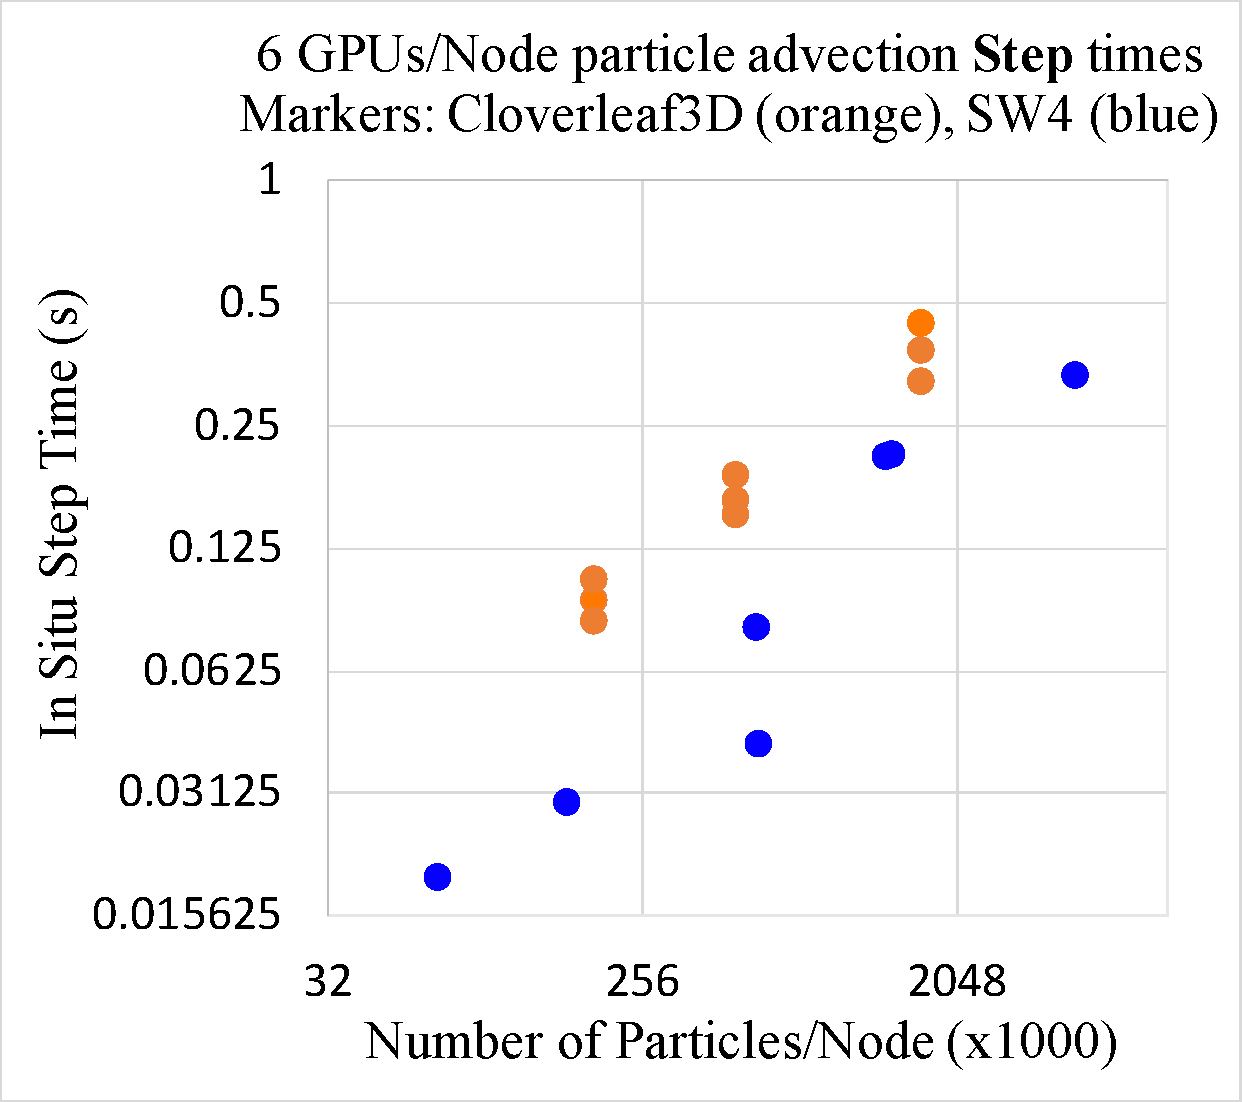
\includegraphics[width=0.93\linewidth]{images/GPU_Step.pdf}}\\
\cline{1-9}
\multirow{9}{*}{16} & \multirow{9}{*}{96} & \multirow{9}{*}{$586\times586\times586$} & 20 & 4.73 & \multirow{3}{*}{1.5M} & \multirow{3}{*}{40.2 } & 0.4475 & 9.408 & \\
\cline{4-4}
& & & 40 & 4.08 & & & 0.3221 & 7.894 & \\
\cline{4-4}
& & & 60 & 4.39 & & & 0.3838 & 8.742 & \\
\cline{4-6}%\cline{6-6}
& & & 20 & 4.50 & \multirow{3}{*}{474k} & \multirow{3}{*}{12 } & 0.1882 & 4.182 & \\
\cline{4-4}
& & & 40 & 4.14 & & & 0.1628 & 3.932 & \\
\cline{4-4}
& & & 60 & 4.33 & & & 0.1498 & 3.459 & \\
\cline{4-6}%\cline{6-6}
& & & 20 & 4.19 & \multirow{3}{*}{186k} & \multirow{3}{*}{4.2 } & 0.0925 & 2.207 & \\
\cline{4-4}
& & & 40 & 4.11 & & & 0.1043 & 2.537 & \\
\cline{4-4}
& & & 60 & 3.87 & & & 0.0830 & 2.144 & \\
\cline{1-9}
%\multicolumn{9}{l}{} & \\
\multicolumn{9}{l}{\textbf{          SW4 Seismic Modeling Simulation }} & \\
\cline{1-9}
\multirow{3}{*}{1} & \multirow{3}{*}{6} & $251\times251\times70$ & \multirow{7}{*}{200} & 0.35 & 555k & 13.89 & 0.0412 & 11.67 & \\
\cline{3-3}\cline{5-6}
& & $335\times335\times93$ & & 2.02 & 1.3M & 33.16 & 0.2125 & 10.48 & \\
\cline{3-3}\cline{5-6}  
& & $501\times501\times139$ & & 7.58 & 4.4M & 111.13 & 0.3309 & 4.365 & \multirow{13}{*}{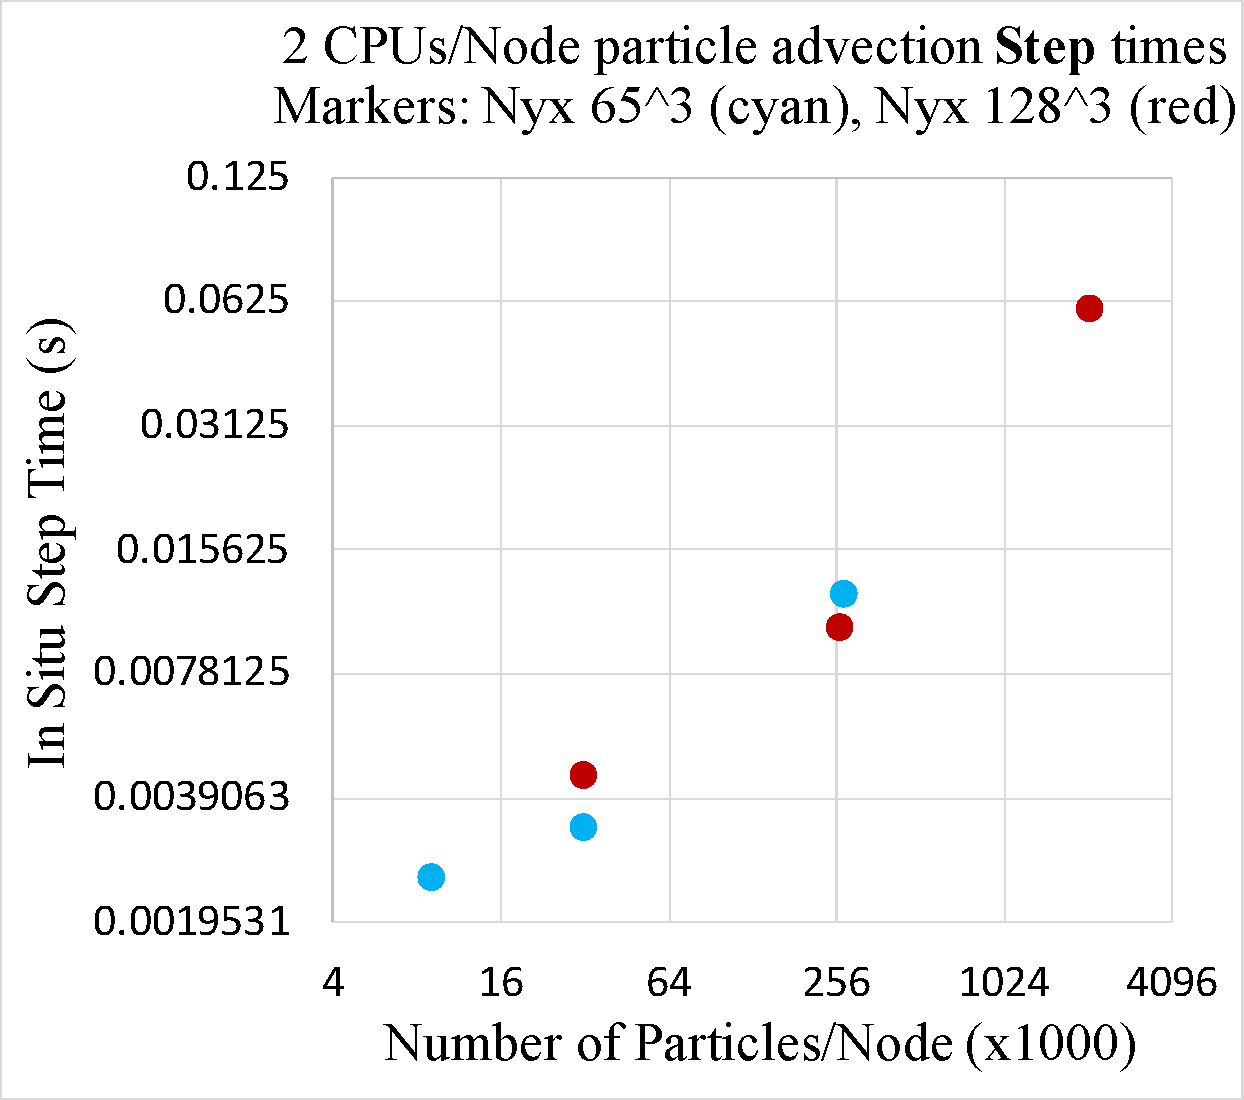
\includegraphics[width=0.93\linewidth]{images/CPU_Step.pdf}}\\
\cline{1-3}\cline{5-6}
\multirow{4}{*}{64} & \multirow{4}{*}{384} & \multirow{3}{*}{$1001\times1001\times276$} & & 1.6 & 66k & 1.6 & 0.0194 & 1.201 &  \\
\cline{6-6}
& & & & 1.5 & 146k & 3.6 & 0.0295 & 1.944 & \\
\cline{6-6}
& & & & 1.3 & 540k & 13.5 & 0.0798 & 6.175 & \\
\cline{3-3}\cline{5-6}
& & $1335\times1335\times368$ & & 2.9 & 1.2M & 31.9 & 0.2095 & 7.074 & \\
\cline{1-9}
%\multicolumn{9}{l}{} & \\
\multicolumn{9}{l}{\textbf{          Nyx Cosmology Simulation }} & \\
\cline{1-9}
\multirow{6}{*}{1} & \multirow{6}{*}{1} & \multirow{3}{*}{$65\times65\times65$} & \multirow{6}{*}{100} & \multirow{3}{*}{10.9} & 274k & 6.8 & 0.0122 & 0.112 & \\
\cline{6-6}
& & & & & 32k & 0.8 & 0.0033 & 0.030 & \\
\cline{6-6}
& & & & & 9k & 0.2 & 0.0025 & 0.023 & \\
\cline{3-3}\cline{5-6}
& & \multirow{3}{*}{$129\times129\times129$} & & \multirow{3}{*}{88.3} & 2.1M & 53.6 & 0.0596 & 0.067 & \\
\cline{6-6}
& & & & & 262k & 6.5 & 0.0101 & 0.011 & \\
\cline{6-6}
& & & & & 32k & 0.8 & 0.0044 & 0.005 & \\
\hline
\end{tabular}
\vspace{-3mm}
\caption{\textit{In situ} encumbrance evaluation and experiment configurations for our three simulation codes.}
\label{table:encumbrance}
\vspace{-5mm}
\end{table*}
\endgroup


This section provides an overview of our experiments.
%
It is organized as follows: 
experiments performed (\ref{sec:experiments}), simulation codes~(\ref{sec:datasets}),
software implementation (\ref{sec:infra}),
hardware (\ref{sec:runtime}),
and metrics (\ref{sec:metrics}).

\subsection{Experiment Overview}
\label{sec:experiments}

Our experiments are designed in response to the evaluation ``areas''
from Section~\ref{sec:instantiation}.
%
Since our evaluations can be separated into two distinct phases, 
we organized our experiments into two distinct campaigns (one for
\textit{in situ} encumbrance and one \textit{post hoc} efficacy),
although some of the
experiments were used in both campaigns.
%

Our experiments considered five basic factors:
\begin{tightItemize}
\item Simulation code
\item Number of particles (Lagrangian basis flows)
\item Interval (number of cycles between saves)
\item Grid size
\item Concurrency
\end{tightItemize}
\noindent
For each factor, there are many possible options.
%
Therefore, running experiments for the cross-product of options
was prohibitive, especially since we had limited time on our supercomputer
(1000 node hours).
%
Instead, we sampled the space of possible options.
%
For both campaigns, our organization was around our three
simulation codes: Cloverleaf3D, SW4, and Nyx 
(described in subsection~\ref{sec:datasets}).
%
For a given simulation code, we varied some factors and fixed others.
%
Our goal was to simultaneously
 provide coverage and yet allow us to see the impact of certain factors,
all while staying within our compute budget.
%
In all, we ran 47 experiments, 22 for \textit{in situ} encumbrance and 25
for \textit{post hoc} efficacy.
%
Table~\ref{tab:campaign1} shows our choices for the \textit{in situ}
encumbrance campaign, while Table~\ref{tab:campaign2} shows
our choices for the \textit{post hoc} efficacy campaign.
%
Specific choices for options 
%(e.g., how many Lagrangian basis flows are used for Cloverleaf3D?) 
are documented in the Results section.

\begin{table}[h]
\centering
\vspace{-2mm}
\scalebox{0.9}{
\begin{tabular}{|r||c|c|c|c|c|}
\hline
Simulation Code & Cloverleaf3D & SW4 & Nyx \\ \hline
\# of Particles  &   3 & 3 & 3 \\
Interval &  3 & 1 & 1 \\
Grid Size & 1 & 3,2 & 2 \\
Concurrency & 1 & 2 & 1 \\  \hline
Total Experiments & 9 & 7 & 6 \\ \hline
\end{tabular}
}
\vspace{-3mm}
\caption{\label{tab:campaign1}Experimental overview for the \textit{in situ} encumbrance campaign.  For SW4, we were able to run a very fine grid size at low concurrency, but not the entire cross product of options due to limitations in compute time.  Overall, we considered 22 experiments for this campaign.}
\end{table}

\begin{table}[h]
\centering
\scalebox{0.9}{
\begin{tabular}{|r||c|c|c|c|c|}
\hline
Simulation Code                  & Cloverleaf3D & SW4 & Nyx \\ \hline
\# of Particles  &   3 & 4 & 3 \\
Interval &  3 & 1 & 4 \\
Grid Size & 1 & 1 & 1 \\
Concurrency & 1 & 1 & 1 \\  \hline
Total Experiments & 9 & 4 & 12 \\ \hline
\end{tabular}
}
\vspace{-3mm}
\caption{\label{tab:campaign2}Experimental overview for the post hoc efficacy campaign.
%
Overall, we considered 25 experiments for this campaign.}
\end{table}


%The remainder of this subsection describes the simulation codes we study
%(\ref{sec:datasets}) and the motivation for studying the other factors (\ref{sec:parameters}).

\subsection{Simulation Codes}
\label{sec:datasets}
For our study we consider three simulation application codes that are used and/or developed as part of the 
Exascale Computing Project from the
United States Department of Energy.
%

First, we use the Cloverleaf3D~\cite{mallinson2013cloverleaf} mini or proxy ECP application that solves compressible Euler equations in a hydrodynamics setting on a Cartesian grid using an explicit second-order method. 
%
Cloverleaf3D has been developed and used by several studies to evaluate emerging architectures and various techniques targeting Exascale applications.
%
The simulation is initially relatively stable and begins with an energy bar expanding from the center of the XY plane along the Z-axis. 
%
Figure~\ref{fig:teaser}a show pathlines calculated in the Cloverleaf3D domain that show this initial behavior in the simulation.

Next, we consider the SW4 seisomology simulation~\cite{petersson2015wave}.
%
This is an ECP application developed to study seismic wave propagation.
%
It operates and produces multiple domains with a time-dependent displacement field depending on the input deck provided to it.
%
We operate on a single domain and use the displacement vector field as input to our \textit{in situ} Lagrangian operator.
%
Figure~\ref{fig:teaser}b is generated by visualizing the displacement magnitude of the particle trajectories extracted over the first 1000 cycles.
%
%\fix{remove these sentences?:}
%The visualization uses line contours, with each node selecting 10 isovalues for the range of displacement magnitude in the node.
%
%The color map range is the same for the entire domain, i.e., all nodes use the same maximum and minimum values.
%

The last data set we consider is the Nyx cosmology simulation~\cite{almgren2013nyx}, another ECP application.
%
The simulation's hydrodynamics is based on a compressible flow formulation in Eulerian coordinates. 
%
We built an Lya executable used to model Lyman-alpha forest in quasar spectra.
%
For this simulation, we derived the velocity field using the fields of momentum and density.
%
%\fix{Too long!}
%Figure~\ref{fig:vectorfield_nyx} shows a slice of the Nyx vector field at two time slices.
%
%We observed that the unit vectors at each grid point remain relatively the same across all cycles.
%
%The evolution of the vector field is in terms of velocity magnitude.
%
%The maximum velocity magnitude in the domain increases steadily for every cycle of the application we simulated.
%
%Further, Figure~\ref{fig:pathlines_nyx} is a visualization of the volume of the domain using 100,000 randomly seeded pathlines integrated for the first 25 cycles of the simulation.
%
%\begin{figure}[h]
\centering
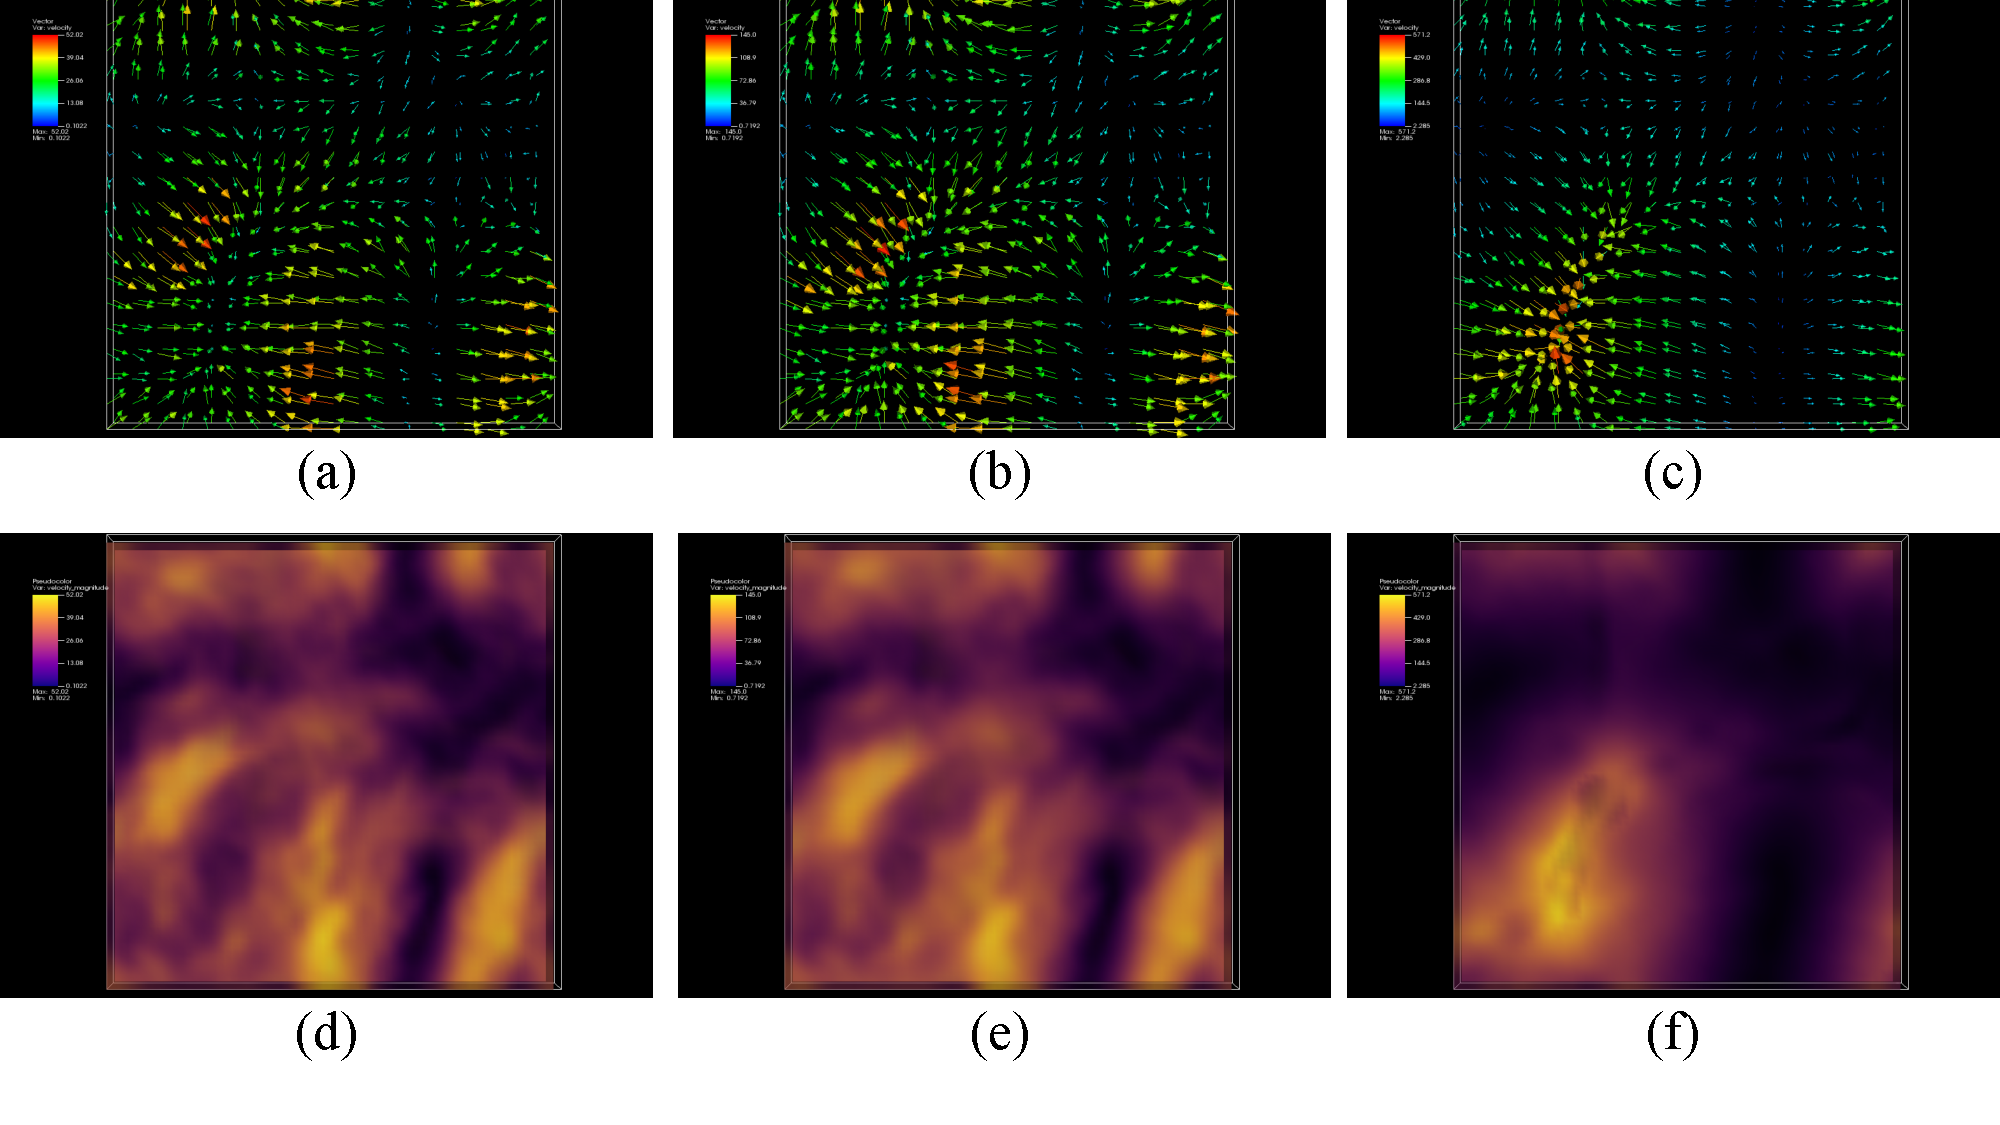
\includegraphics[width=1\linewidth, trim={0cm 1.1cm 0cm 0cm}, clip]{images/Nyx_vectorfields.pdf}
\vspace{-5mm}
\caption{Nyx vector field visualization: (a) and (d) show the vector field at time 0 and the maximum velocity magnitude is 52.02, (b) and (e) show the vector field at time 200 and the maximum velocity magnitude is 145.0, and finally, (c) and (f) show the vector field at time 400 and the maximum velocity is 571.2.}
\label{fig:vectorfield_nyx}
\vspace{-3mm}
\end{figure}





%\subsubsection{Parameter Space}
%\label{sec:parameters}

%We vary the different ``knobs'' in the parameter space to evaluate the viability and efficacy of using in situ Lagrangian analysis to perform exploratory time-dependent vector field analysis and visualization. 
%
%Our study considers the following parameters:
%\begin{itemize}
%\item \textbf{Number of particles:} Our study varies the number of particles initialized per node and thus inform the cost of performing particle advection for varying workloads every cycle of the simulation. Further, the number of particles initialized is directly impacts the size of the data stored to disk and the accuracy of the reconstruction.
%%
%We specify the number of particles initialized using the notation \textbf{1:X}, where X is the reduction factor. 
%%
%For example, a 1:1 configuration states that one particle is used for every grid point (no reduction) and a 1:8 configuration states that one particle is used for every 8 grid points (12.5\% of the original data size). 
%%
%\item \textbf{Interval:} We consider the interval or frequency at which files are stored to disk. 
%%
%For a given total number of simulation cycles, this impacts the total amount of data stored to disk. 
%%
%Additionally, for the Lagrangian representation, the interval is directly related to the integration length of each massless particle. 
%%
%%For each configuration, we specify the number of cycles between storing to disk and refer to this as the \textbf{interval}. 
%%
%\item \textbf{Grid size:} We consider different grid sizes to measure the in situ encumbrance of varying workloads. 
%%
%Different grid sizes will use a different number of particles to sample the domain reasonably accurately.
%%
%In particular, we are interested in the in situ encumbrance when a single compute node is operating on a large number of grid points.
%
%\item \textbf{Concurrency:} We consider the costs at various scale (i.e., number of compute nodes, MPI ranks). Further, the simulation codes required different parallelization hardware and thus, across simulation codes we measure the costs of Lagrangian representation extraction using, both, GPUs and CPUs for particle advection.
%\end{itemize}

\subsection{Software Implementation}
\label{sec:infra}
\subsubsection{In Situ Reduction}
\label{sec:insituimp}
We use the Ascent~\cite{larsen2017alpine} \textit{in situ} infrastructure and VTK-m~\cite{moreland2016vtk} library to implement \textit{in situ} data reduction via by calculating a Lagrangian representation. 
%
%Lagrangian analysis is implemented as an extraction filter in VTK-m. 
%
%For each of the simulation codes we consider, Ascent is first integrated with the simulation code.
%
%Ascent can be configured to perform Lagrangian analysis when the simulation is executed.
%
%The specifics of an analysis configuration are input to Ascent using either a json or yaml file.
%
%The Lagrangian analysis filter requires parameters specifying seed resolution, frequency of storing information to disk, the name of the vector field, and step size.
%%
%Ascent passes the simulation velocity data to the Lagrangian filter via VTK-h~\cite{larsen2017alpine}, a distributed memory wrapper around VTK-m, every cycle. 
%
%Further, we use utilities within Ascent to measure timings and to strip simulation data of ghost zones.
%
The VTK-m Lagrangian filter on each rank operates independently and maintains its own list of basis particles and uses the existing particle advection infrastructure available in VTK-m~\cite{pugmire2018performance}.
%
RK4 particle advection is implemented using VTK-m worklets (kernels or functors) that offer performance portability by utilizing the underlying hardware accelerators. 
%
%The Lagrangian filter operates across simulation cycles and stores one value in memory for each basis flow seed particle: current position (x, y, z).
%
In our implementation, each Lagrangian filter stores the displacement of each particle (3 double), as well as its validity (1 boolean), i.e., whether the particle remained within the domain during the interval of calculation.
%
%The validity of a particle is essential to consider when searching for a valid interpolation neighborhood during post hoc reconstruction.
%
%Our implementation computes the displacement and validity using VTK-m worklets as a final step before adding both fields to the output data set object. 
%
In more complicated frameworks, it is possible to associate additional information (for example, ID, age, start location, previous locations, etc.) with each particle at the cost of higher runtime memory usage and data storage.
%
%For our study, we store data in a VTK ASCII file format for structured grids.
%
%Figure~\ref{} is a schematic diagram of the infrastructure and shows the relation of \textit{in situ} Lagrangian analysis to the simulation code.

We use Ascent to store the complete velocity field at a specified frequency in order to evaluate the traditional Eulerian paradigm.
%
%Similar to the Lagrangian filter, we store data in a VTK ASCII file format for structured grids.
%
For every Eulerian configuration, we store the full spatial resolution of the simulation domain under consideration. 
%

\subsubsection{Post Hoc Exploration}
We build two parallelize-over-data distributed-memory \textit{post hoc} interpolation pipelines, one for each: Lagrangian and Eulerian.
%
%To calculate pathlines using the Lagrangian data post hoc, a particle $p$ identifies a neighborhood of basis flows to follow.
%
%A neighborhood is the convex hull that contains the location of the $p$.
%
For the Lagrangian \textbf{PHE} we construct a search structure in the form of a Delaunay triagulation over the start locations of valid basis particles using CGAL~\cite{fabri2011cgal} to identify particle neighborhoods.
%We calculate the Delaunay triangulation over all the start locations of valid basis flows using CGAL~\cite{fabri2011cgal}.
%
%Thus, we locate particle neighborhoods by identifying the containing cell in the Delaunay triangulation. 
%
%We choose to use a reconstruction method that can operate on structured, as well as unstructured data, because Lagrangian representations can take many forms.
%
%Use of a method that supports unstructured input, i.e., the basis particles are not initialized along a uniform grid, provides a better representation of the general post hoc reconstruction case.
%
%The most straightforward, albeit expensive, approach is to calculate a global Delaunay triangulation.
%
%However, a global Delaunay triangulation can get prohibitively expensive as the total number of particles increases.
%
%A second approach is to perform spatial binning followed by a smaller more local Delaunay triangulation.
%
%However, this method requires an expanding search structure in addition to a binning scheme to guarantee a particle locates a neighborhood if available.
%
%Further, the cost of calculating a local Delaunay triangulation for each particle would be dependent on the number of particles.
%
In our implementation, each rank loads basis particles of the rank itself as well as basis particles generated by spatially adjacent ranks (i.e., upto 27 ranks for a rectilinear simulation grid).
%
%Thus, each post hoc interpolation rank loads data from upto 27 ranks.
%
%The Delaunay triangulation is then performed for all the valid basis flows in the loaded data.
%
%Although not optimal, this approach will scale better than a global Delaunary triangulation while remaining straightforward.
%
%The best approach to identify a particle neighborhood in a large distributed memory settings with a large number of particles remains an open research problem and is beyond the scope of this work. 
%
Once a particle neighborhood is identified, barycentric coordinate interpolation is used to calculate the displacement of $p$.  
%
%If a particle enters the domain bounds of an adjacent node it is communicate to the rank corresponding to that domain using MPI. 
%
Our implementation uses MPI to communicate particles across ranks and continue the integration of trajectories across node boundaries.

For the Eulerian \textit{post hoc} interpolation pipeline, we use the VTK-m particle advection infrastructure to perform RK4 integration and MPI for communication of particles across ranks.
%
%In this pipeline, each rank is only required to load the velocity field stored to disk for that particular rank.


%We ran with VTK-m in Ascent.

\subsection{Runtime Environment}
\label{sec:runtime}
Our empirical study uses the Summit supercomputer at ORNL. 
%
A Summit compute node has two IBM Power9 CPUs, each with 21 cores running at 3.8 GHz and 512 GBytes of DDR4 memory. 
%
Nodes on Summit also have enhanced on-chip acceleration with each CPU connected via NVLink to 3 GPUs, for a total of 6 GPUs per node. 
%
Each GPU is an NVIDIA Tesla V100 with 5120 CUDA cores, 6.1 TeraFLOPS of double precision performance, and 16 GBytes of HBM2 memory.
%
Lastly, it uses a Mellanox EDR 100G InfiniBand, Non-blocking Fat Tree as its interconnect topology.

%Alaska is the small cluster at our research lab.
%%
%The head node with consists of two Intel Xeon E5-2667v3 CPU, each with 16 cores running at 3.2 GHz. 
%
%We use Summit to build, integrate, and execute in situ Lagrangian analysis with simulation codes.
%%
%Thus, all of our in situ extraction is performed on Summit. 
%%
%Additionally, we use Summit to perform large distributed memory post hoc reconstructions.
%%
%We use Alaska for the smaller post hoc reconstruction processes.



%Most of our experiment test configurations have two phases: in situ and post hoc. 
%
%The performance characteristics of the in situ phase is what we are primarily interested in.
%
%We execute extra ``only-extraction'' configurations to gauge in situ performance and that do not continue to the post hoc phase.
%
%The post hoc phase in our study is used to measure accuracy.
%
%We report timings associated with performing post hoc Lagrangian reconstruction on a single node and in a distributed memory setting.
%
%We strongly believe that as in situ Lagrangian representations evolve, the post hoc techniques used will as well.
%
%Currently, to the best of our knowledge there does not exist a perfect one-size-fits-all post hoc Lagrangian-based advection method.

%\begin{figure}[t]
\centering
%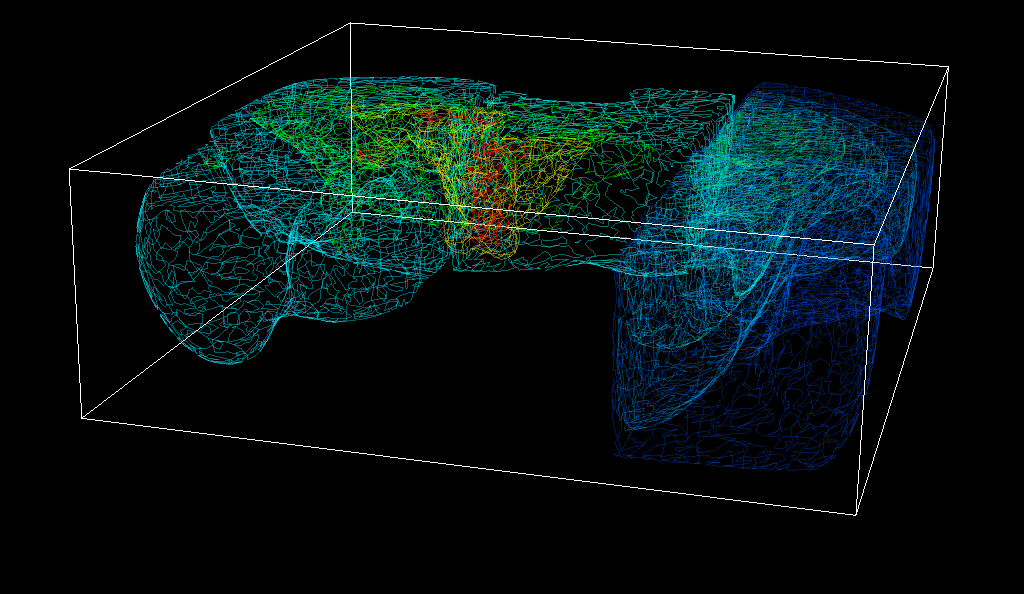
\includegraphics[width=0.8\linewidth]{images/sw4_vis_2.png}
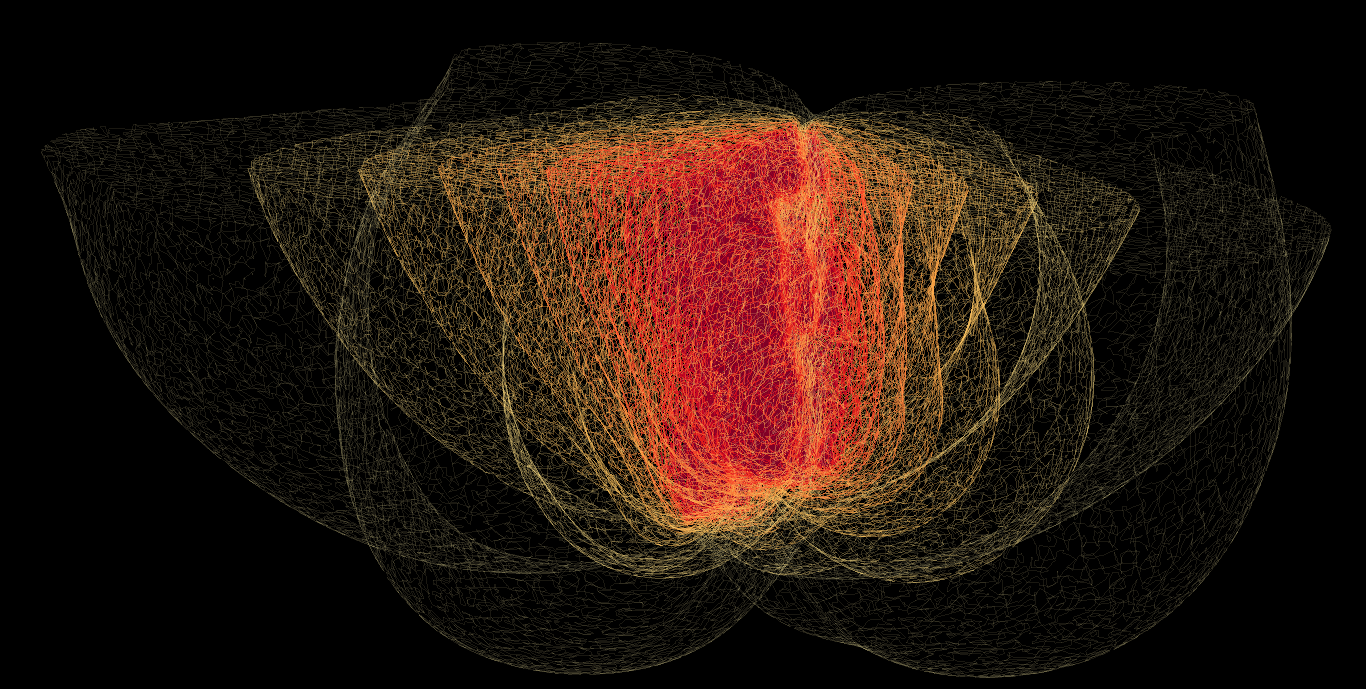
\includegraphics[width=0.8\linewidth]{images/sw4_waves.png}
\caption{SW4 wave propagation visualization}
\label{fig:sw4_vis}
\end{figure}



%\begin{figure}[t]
\centering
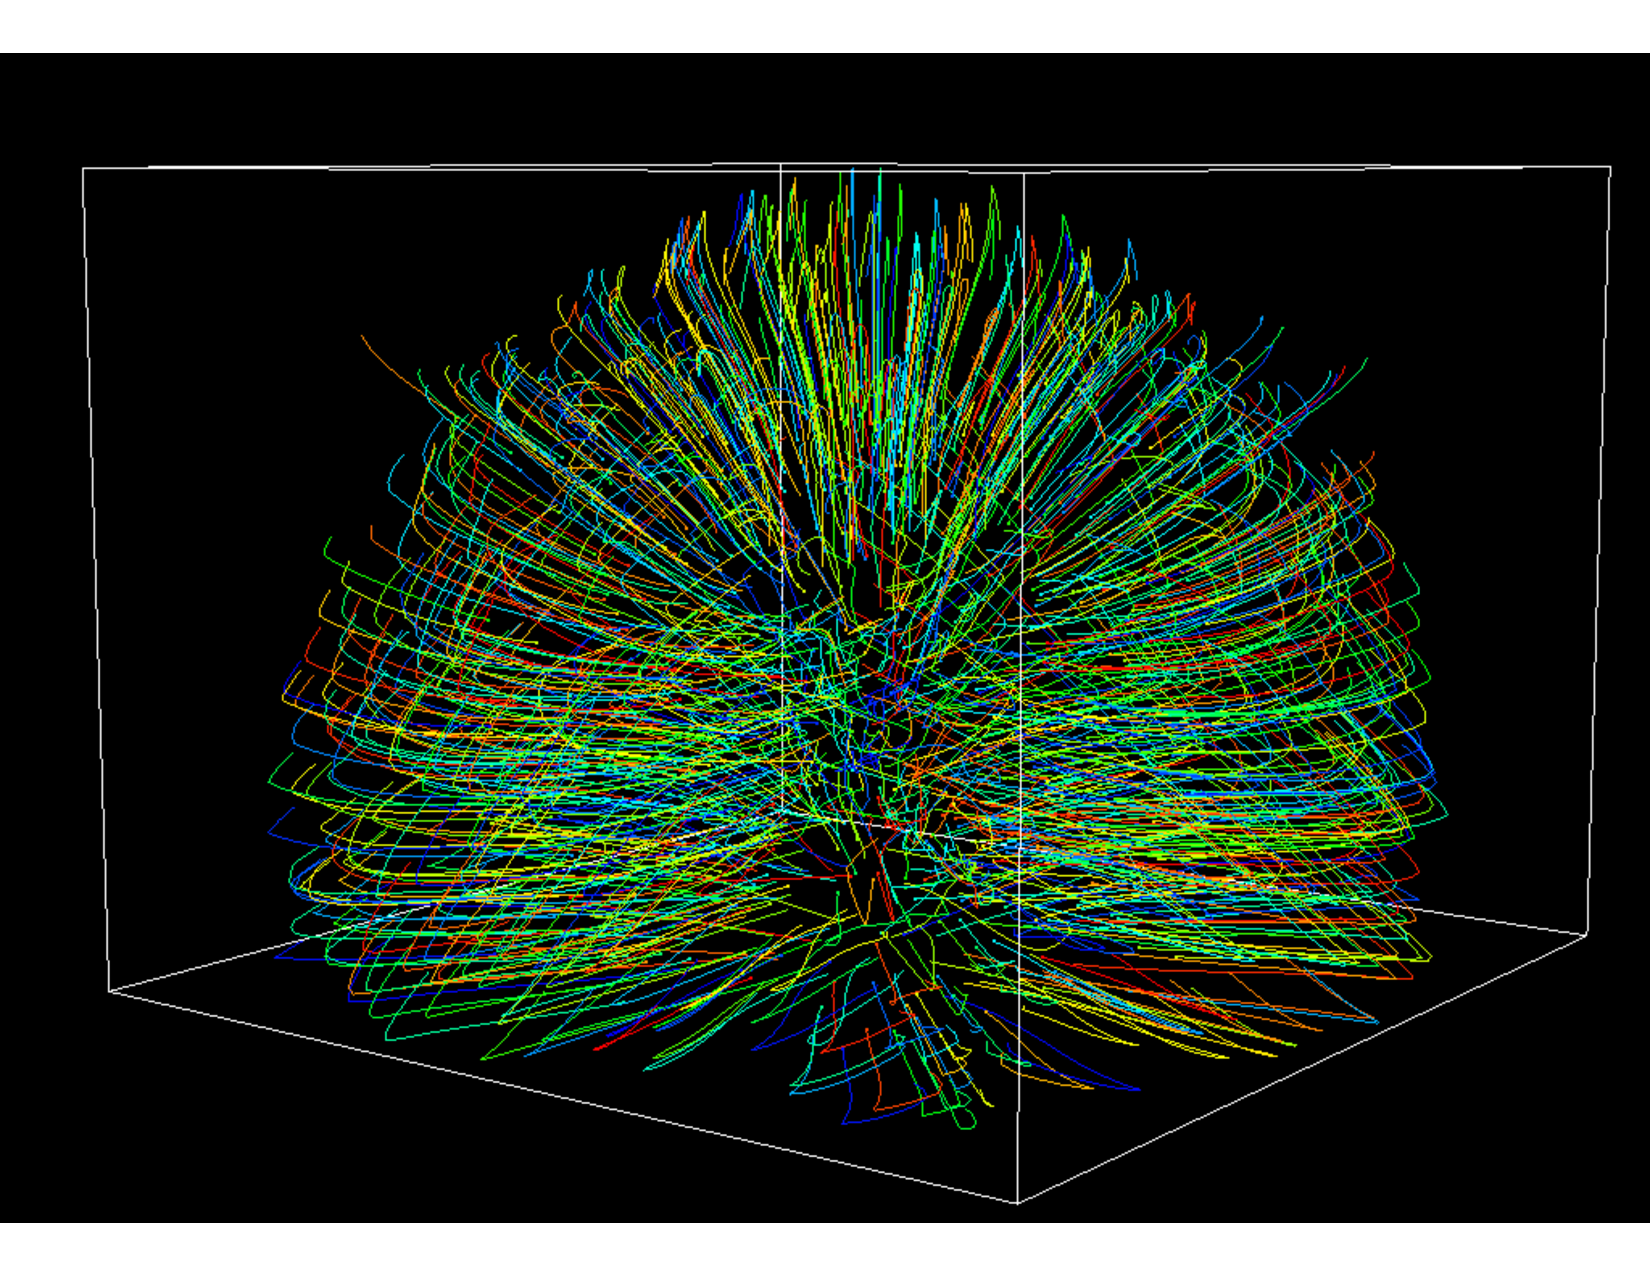
\includegraphics[width=0.7\linewidth]{images/pathlines_clover.pdf}
\caption{Cloverleaf3D flow visualization}
\label{fig:pathlines_clover}
\end{figure}



%\begin{figure}[t]
\centering
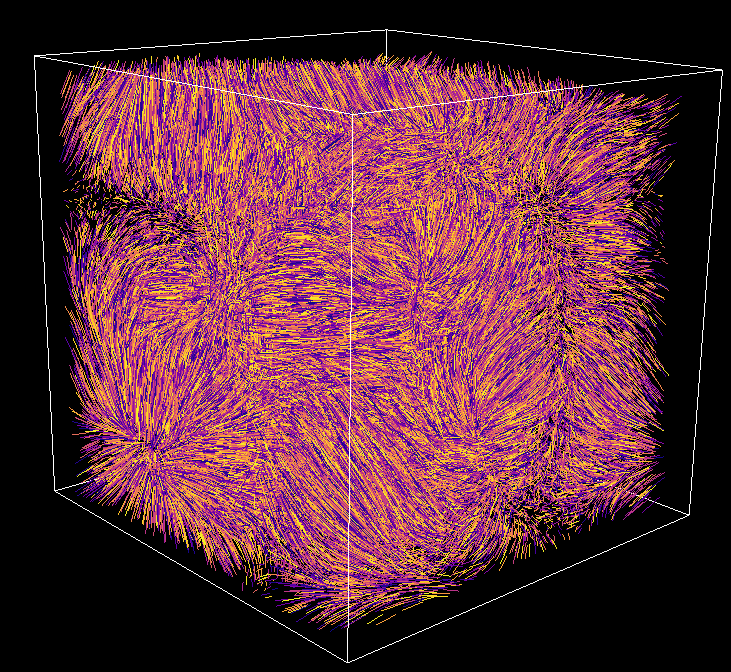
\includegraphics[width=0.65\linewidth]{images/pathlines_nyx.png}
\caption{Nyx flow visualization: 100,000 randomly seeded pathlines calculated for the first 25 cycles of the simulation.}
\label{fig:pathlines_nyx}
\end{figure}




\subsection{Evaluation Metrics}
\label{sec:metrics}

\subsubsection{In Situ Encumbrance}
\label{sec:encumbrance}
%
Our empirical study measures \textit{in situ} encumbrance in terms of execution time and memory usage.
%
For \textbf{ISR-1}, we measure the cost of each invocation of the Lagrangian VTK-m filter and report the average time, i.e., cost of particle advection for one cycle or \textbf{Step}.
%.
Additionally, we measure and report the percentage of simulation time spent on data analysis and visualization routines, or \textbf{DAV\%}.
%
For this we consider the simulation cycle time or Sim$_{cycle}$.
For \textbf{ISR-2}, we measure the runtime memory cost incurred by every compute node to maintain the state (current position) of particles at runtime in Bytes.


\subsubsection{I/O Cost}
\label{sec:iocost}
In this empirical study, we do not report or factor the cost of I/O write times. 
%
Besides being an operation that is performed infrequently in our case, 
we observed for the scale of study we conducted that Summit provides very 
fast write times.
%
Table~\ref{table_binary} documents write times of varying file sizes in binary format on Summit.
%
\begin{table}[h]
\centering
\vspace{-2mm}
\scalebox{0.9}{
\begin{tabular}{||c||c|c||}
\hline
File Size (MB) &  1 MPI/Node~(s) & 6 MPI/Node~(s) \\
\hline
1 & 0.0018 & 0.0022 \\
\hline
%5 & 0.0016 & 0.01 \\
%\hline
10 & 0.0032 & 0.0045 \\
\hline
%20 & 0.0054 & 0.0078 \\
%\hline
50 & 0.0064 & 0.013 \\
\hline
100 & 0.0125 & 0.038 \\
\hline
200 & 0.0231 & 0.171 \\
\hline
\end{tabular}
}
\vspace{-2mm}
\caption{Write time measurements for various file sizes (in binary format) to disk on Summit. We consider two cases: one MPI rank or six simultaneous MPI ranks each writing the file to disk on a single compute node. For each timing, we average over multiple runs and every timing is reported in seconds.}
\label{table_binary}
\vspace{-3mm}
\end{table}

Given the range of file sizes stored to disk by a single MPI rank in our empirical study is between 0.5 MB to 115 MB, we believe this cost is negligible at the scale that we test (and perhaps, even at larger scales).
%
Thus, we limit our measurement and discussion of I/O to the total data storage required on the file system and report \textbf{DS-1} in Bytes stored.

%Of course, I/O costs might be relevant if the operation was frequent at full scale --- all the nodes with several MPI ranks each trying to write at the same time. 
%
%However, 

%We discuss our reasoning for this below. 
%
%When writing to a binary format we observed very fast write times on Summit. 
%%
%Summit is designed to provide low access latency and high bandwidth. 
%%
%We found that a binary file of size 200 MB can be written in 0.0231 seconds on a single compute node running a single MPI task. 
%%
%And it takes 0.171 seconds of wall time for 6 MPI ranks to each write 200 MB files in parallel. 
%%
%In our experiments the largest file stored to disk by a single rank for a single interval or cycle is 115 MB. 
%%
%The range of sizes varies from 0.5 MB to 115 MB per node per instance of storing to disk (0.002 to 0.04 seconds, respectively). 
%%
%We provide some of these timings for reference in Table~\ref{table_binary}.
%%
%Further, this infrequent operation and small cost of I/O in comparison 
%to the cost of a particle advection step which is performed each cycle is small.

%Although write times may be impacted at full scale --- all the nodes with several MPI ranks each trying to write at the same time - a study of this scale is beyond the scope of this work and more oriented toward a supercomputer I/O performance study. 
%
%Further, in our relatively small study to inform ourselves, we found noise that we attribute to the cluster running hundreds of jobs simultaneously to be significant. 

%Further, since \textbf{L-ISR} in intended to be used as a data reduction operator, the sizes of files written to disk would be approximately the same size (1:1) or significantly smaller (1:8, 1:27, 1:64). 
%
%If I/O costs were to be impacted, either due to scale or file format type, then the cost of Eulerian would be more adversely affected if compared against a reduced Lagrangian I/O cost. 
%

%Another point to consider is the infrastructure performing the operation of storing data. 
%
%Depending on whether the data is being written to a burst buffer or some staging platform before moving data to permanent storage can significantly alter the value of these timings. 

%All this being said, at scale scientists will not choose to save all the data due to excessive storage costs and since this would then indeed introduce a large cumulative encumbrance. 
%
%Instead, they resort to temporal subsampling, i.e., saving data out at a predetermined frequency or at select cycles. 
%
%One of our key assumptions is that as data sizes get larger, scientists will be forced to save less frequently or to store reduced data sets. 





\subsubsection{Post Hoc Efficacy}
\label{sec:evaluation}
Our empirical study measures time-dependent vector field reconstruction error by evaluating the accuracy of test particles trajectories interpolated using the extracted Lagrangian representation.
%
%For our Cloverleaf3D and Nyx experiments, we randomly place 100,000 and 50,000 test particles in the domain respectively.
%
%For the SW4 experiments, we place 90,000 test particles randomly in between $Z=5000$ and $Z=15,000$ (layer of activity in the domain).
%

For \textbf{PHE-1}, our empirical study measures the L2-norm, i.e., the Euclidean distance, for each interpolated point and compares it to a ground truth that is precomputed using the complete simulation data. 
%
We use \textbf{Avg$_{L2}$} and \textbf{Max$_{L2}$} to denote the average and maximum L2-norm for an individual particle trajectory, respectively.
%
%We note, the Max$_{L2}$ was similar to the end point distance between the ground truth and test particle trajectories.
%

An overall average of \textbf{Avg$_{L2}$}, denoted by \textbf{AvgN$_{L2}$}, is measured across $N$ test particle samples and provides a robust statistic~\cite{agranovsky2014improved, sane2018revisiting, sane2019interpolation, rapp2019void}.
%
Unlike \textbf{AvgN$_{L2}$}, a maximum error is more susceptible to outliers that could arise from small but complex regions of flow.
%
To provide a more detailed quantitative analysis compared to prior work, we use histograms to capture the distribution of error~(\textbf{Avg$_{L2}$}, \textbf{Max$_{L2}$}) across all test particles and provides insight into per particle outcomes.  
%
Further, for \textbf{PHE-2} we include a study of \textit{post hoc} reconstruction costs. 

%\begingroup
\setlength{\tabcolsep}{0pt}
%\renewcommand{\arraystretch}{0.55} % Default value: 1
%\setlength{\fboxsep}{1mm}
\begin{table*}[t]
\centering
\begin{tabular}{|P{2cm}|P{1.3cm}|P{2cm}|L{1.3cm} P{1.7cm} D |P{8cm}|}
\hline
Technique & Interval & Reduction & Data & AvgN$_{L2}$ & Cell  & \multirow{2}{*}{Scatter Plot} \\
& & & & & Side\% & \\
\hline
\multicolumn{6}{l}{\textbf{          Cloverleaf3D Proxy Hydrodynamics Application }} & \multirow{12}{*}{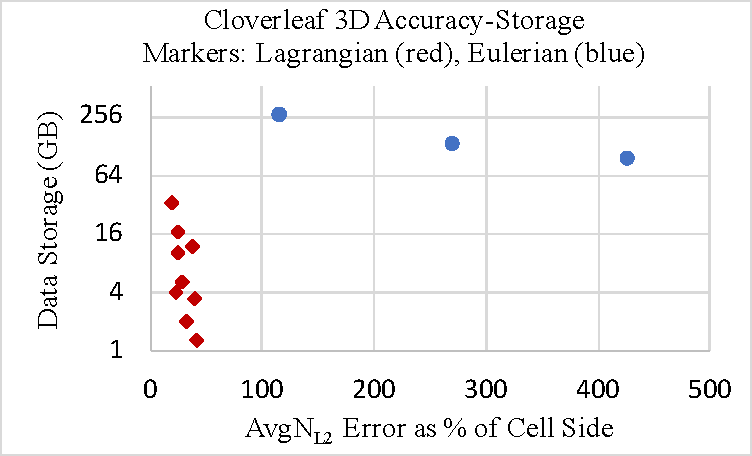
\includegraphics[width=0.95\linewidth]{images/cloverleaf_accuracy.pdf}}\\
\cline{1-6}
\multirow{3}{*}{Eulerian} & 20 & \multirow{3}{*}{Full Res} & 267 GB & 0.0197 & 116.17 &  \\
\cline{2-2}
& 40 & & 133 GB & 0.0459 & 270.49 & \\
\cline{2-2}
& 60 & & 95 GB & 0.0725 & 426.96 &  \\
\cline{1-6}
\multirow{9}{*}{Lagrangian} & \multirow{3}{*}{20} & 1:8 & 34 GB & 0.0032 & 18.928 & \\
\cline{3-3}
 & & 1:27 & 10 GB & 0.0040 & 23.891 & \\
\cline{3-3}
 & & 1:64 & 4 GB & 0.0040 & 23.583 & \\
\cline{2-3}
& \multirow{3}{*}{40} & 1:8 & 17 GB & 0.0043 & 25.646 &  \\
\cline{3-3}
& & 1:27 & 5.1 GB & 0.0049 & 29.145 &  \\
\cline{3-3}
& & 1:64 & 2 GB & 0.0053 & 31.353 & \\
\cline{2-3}
& \multirow{3}{*}{60} & 1:8 & 12 GB & 0.0064 & 37.882 & \\
\cline{3-3}
& & 1:27 & 3.4 GB & 0.0066 & 39.002 & \multirow{6}{*}{\raisebox{-33.5mm}[0pt][0pt]{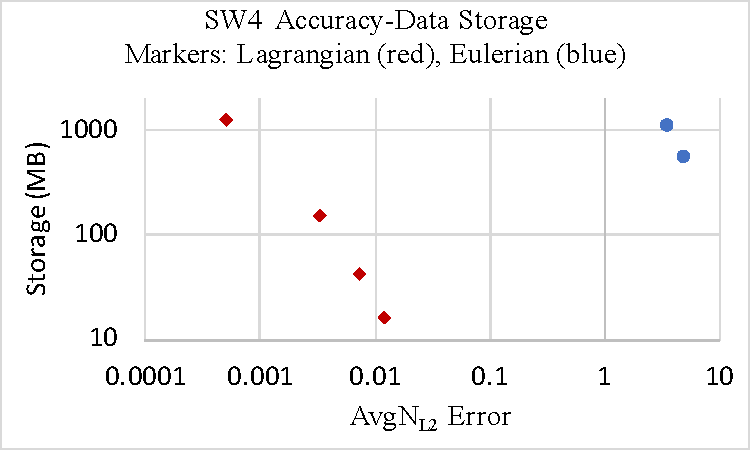
\includegraphics[width=0.95\linewidth]{images/sw4_accuracy.pdf}}} \\
\cline{3-3}
& & 1:64 & 1.3 GB & 0.0070 & 41.247 & \\
\cline{1-6}
\multicolumn{6}{l}{\textbf{          SW4 Seismic Wave Modeling Simulation }} &  \\
\cline{1-6}
\multirow{2}{*}{Eulerian} & 250 & \multirow{2}{*}{Full Res} & 1100 MB & 3.5714 & 0.9224 & \\
\cline{2-2}
 & 500 & & 550 MB & 5.0493 & 1.3023  & \\
\cline{1-6}
\multirow{4}{*}{Lagrangian} & \multirow{4}{*}{250} & 1:1 & 1300 MB & 0.0005 & 0.0001  &  \\
\cline{3-3}
 &  & 1:8 & 158 MB & 0.0033 & 0.0008 &  \\
\cline{3-3}
 &  & 1:27 & 42 MB & 0.0072 & 0.0018 & \\
\cline{3-3}
 &  & 1:64 & 16 MB & 0.0128 & 0.0031 &  \\
\cline{1-6}
\multicolumn{6}{l}{\textbf{          Nyx Cosmology Simulation }} & \\
\cline{1-6}
\multirow{4}{*}{Eulerian} & 25 & \multirow{4}{*}{Full Res} & 227 MB & 0.010 & 2.2954 &  \\
\cline{2-2}%\cline{4-6}
& 50 & & 120 MB & 0.037 & 8.4090 &  \multirow{16}{*}{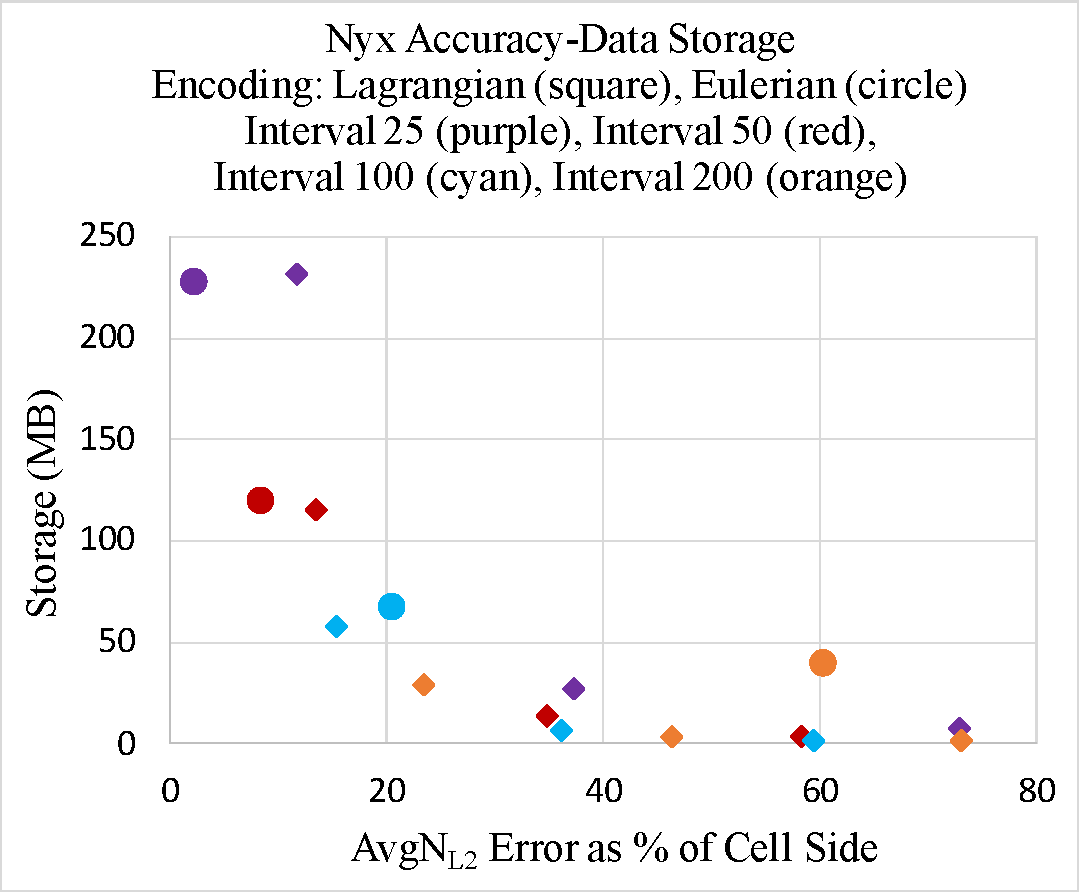
\includegraphics[width=0.95\linewidth]{images/nyx_accuracy.pdf}}\\
\cline{2-2}%\cline{4-6}
& 100 & & 67 MB & 0.090 & 20.454 & \\
\cline{2-2}%\cline{4-6}
& 200 & & 40 MB & 0.265 & 60.227 & \\
\cline{1-6}
\multirow{12}{*}{Lagrangian} & \multirow{3}{*}{25} & 1:1 & 232 MB & 0.051 & 11.613 & \\
\cline{3-3}
& & 1:8 & 27 MB & 0.164 & 37.272 &  \\
\cline{3-3}
& & 1:27 & 8 MB & 0.320 & 72.727 &  \\
\cline{2-3}
& \multirow{3}{*}{50} & 1:1 & 166 MB & 0.059 & 13.409 & \\
\cline{3-3}
& & 1:8 & 14 MB & 0.153 & 34.772 &  \\
\cline{3-3}
& & 1:27 & 4 MB & 0.256 & 58.181 &  \\
\cline{2-3}
& \multirow{3}{*}{100} & 1:1 & 58 MB & 0.067 & 15.227 &  \\
\cline{3-3}
& & 1:8 & 7 MB & 0.159 & 36.136 &  \\
\cline{3-3}
& & 1:27 & 2 MB & 0.261 & 59.318 & \\
\cline{2-3}
 & \multirow{3}{*}{200} & 1:1 & 29 MB & 0.103 & 23.409 &  \\
\cline{3-3}
& & 1:8 & 3.4 MB & 0.204 & 46.363 & \\
\cline{3-3}
& & 1:27 & 1 MB & 0.321 & 72.954 &  \\
\hline
\end{tabular}
\vspace{-3mm}
\caption{\textit{Post hoc} efficacy evaluation and experiment configurations for our three simulation codes.}
\label{table:accuracy}
\vspace{-5mm}
\end{table*}
\endgroup



%\begin{table*}[!h]
\centering
%\resizebox{\linewidth}{!}{%
\scalebox{0.8}{
\begin{tabular}{||c||c|c|c||c|c||b|c|d|b||}
\hline
\textbf{Configuration} & \textbf{Average File Size} & \textbf{Average I/O} & \textbf{Total I/O} & \textbf{Average Filter} & \textbf{Total Filter} & \textbf{Total In Situ} & \textbf{Simulation Time} & \textbf{\% DAV} & \textbf{Memory/Rank} \\
\hline
Eulerian 20 & 89.9 MB & 94.83s & 2939.73s & NA & NA & 2939.73s & 5428s & 54.15\% & NA \\
\hline
Eulerian 40 & 92.7 MB & 97.12s & 1553.92s & NA & NA & 1553.92s & 4088s & 38.01\% & NA \\
\hline
Eulerian 60 & 89.8 MB & 94.66s & 1041.26s & NA & NA & 1041.26s & 3701s & 28.12\% & NA \\
\hline
Lagrangian 20, 1:8 & 12.1 MB & 9.73s & 291.94s & 0.4475s & 268.53s & 560.48s & 3135s & 17.87\% & 6.4 MB \\
\hline
Lagrangian 20, 1:27 & 3.6 MB & 2.8s & 84.21s & 0.1882s & 112.92s & 197.13s & 2785s & 7.07\% & 1.9 MB \\
\hline
Lagrangian 20, 1:64 &  1.4 MB & 1.1s & 33.11s & 0.0925s & 55.55s & 88.66s & 2550s & 3.47\% & 0.78 MB \\
\hline
Lagrangian 40, 1:8 &  12 MB & 9.64s & 144.65s & 0.3221s & 193.27s & 337.92s & 2594s & 13.02\% & 6.4 MB \\
\hline
Lagrangian 40, 1:27 &  3.6 MB & 2.78s & 41.77s & 0.1628s & 97.7s & 139.48s & 2527s & 5.51\% &  1.9 MB \\
\hline
Lagrangian 40, 1:64 &  1.4 MB & 1.1s & 16.52s & 0.1043s & 62.59s & 79.12s & 2483s & 3.18\% &  0.78 MB \\
\hline
Lagrangian 60, 1:8 &  12 MB & 9.72s & 97.22s & 0.3838s & 230.33s & 327.55s & 2736s & 11.97\% &  6.4 MB \\
\hline
Lagrangian 60, 1:27 &  3.6 MB & 2.78s & 27.88s & 0.1498s & 89.90s & 117.78s & 2628s & 4.48\% &  1.9 MB \\
\hline
Lagrangian 60, 1:64 &  1.4 MB & 1.1s & 11.07s & 0.08308s & 49.84s & 60.92s & 2335s & 2.60\% &  0.78 MB \\
\hline
\end{tabular}
}
\caption{Cloverleaf3D data set - $586^3$ grid. Each of these experiment configurations was executed for 600 cycles using 96 MPI tasks distributed across 16 compute nodes. The timings in the table represent the average across all nodes and intervals of calculation. Each node operates on a domain of approximates 2.1 M points.} 
\label{clover_table}
\end{table*}

%\begin{table*}[!h]
\centering
%\resizebox{\linewidth}{!}{%
\scalebox{0.8}{
\begin{tabular}{||c||c|c|c||c|c||b|c|d|b||}
\hline
\textbf{Configuration} & \textbf{Average File Size} & \textbf{Average I/O} & \textbf{Total I/O} & \textbf{Average Filter} & \textbf{Total Filter} & \textbf{Total In Situ} & \textbf{Simulation Time} & \textbf{\% DAV} & \textbf{Memory/Rank} \\
\hline
Eulerian 25 & 13.4 MB & 6.5s & 110.63s & NA & NA & 110.63s & 4498.7s & 2.46\% & NA \\
\hline
Lagrangian 25, 1:1 & 14.5 MB & 8.49s & 135.96s & 0.0131s & 5.27s & 141.23s & 4308.4s & 3.27\% & 6.6 MB \\
\hline
Lagrangian 25, 1:8 & 1.7 MB & 0.98s & 15.7s & 0.0033s & 1.35s & 17.05s & 4452.8s & 0.38\% & 0.78 MB \\
\hline
Lagrangian 25, 1:27 & 0.48 MB & 0.29s & 4.65s & 0.0027s & 1.1s & 5.75s & 4438.9s & 0.12\% & 0.22 MB \\
\hline
Lagrangian 50, 1:1 & 14.5 MB & 8.54s & 68.37s & 0.0132s & 5.29s & 73.66s & 4499s & 1.63\% & 6.6 MB \\
\hline
Lagrangian 50, 1:8 & 1.7 MB & 0.97s & 7.81s & 0.0036s & 1.45s & 9.26s & 4566.3s & 0.20\% & 0.78 MB \\
\hline
Lagrangian 50, 1:27 & 0.48 MB & 0.28s & 2.3s & 0.0025s & 1.01s & 3.31s & 4523.7s & 0.07\% & 0.22 MB \\
\hline
\end{tabular}
}
\caption{Nyx$_{Small}$ data set - $65^3$ grid. Each of these experiment configurations was executed for 400 cycles. The approximate time per simulation cycle is 10s. For these experiment configurations, each Lagrangian step costs less than 0.02\% of the simulation cycle. A single node operates on 274,625 grid points.}
\label{nyx_64_table}
\end{table*}

%\begin{table*}[!h]
\centering
%\resizebox{\linewidth}{!}{%
\scalebox{0.8}{
\begin{tabular}{||c||c|c|c||c|c||b|c|d|b||}
\hline
\textbf{Configuration} & \textbf{Average File Size} & \textbf{Average I/O} & \textbf{Total I/O} & \textbf{Average Filter} & \textbf{Total Filter} & \textbf{Total In Situ} & \textbf{Simulation Time} & \textbf{\% DAV} & \textbf{Memory/Rank} \\
\hline
Eulerian 25 & 101 MB & 48.8s & 146.4s & NA & NA & 146.39s & 6746.3s & 2.17\% & NA \\
\hline
Lagrangian 25, 1:1 & 110 MB & 65s & 195s & 0.0592s & 4.44s & 199.45s & 6820.4s & 2.92\% & 51.5 MB \\
\hline
Lagrangian 25, 1:8 & 14 MB & 8s & 24.2s & 0.0102s & 0.76s & 25s & 6676s & 0.37\% & 6.3 MB \\
\hline
Lagrangian 25, 1:27 & 4 MB & 2.36s & 7s & 0.0044s & 0.33s & 7.42s & 6639.4s & 0.11\% & 0.78 MB \\
\hline
Lagrangian 50, 1:1 & 109 MB & 65.86s & 65.86s & 0.0600s & 3.00s & 68.86s & 4487.8s & 1.53\% & 51.5 MB \\
\hline
Lagrangian 50, 1:8 & 14 MB & 8.21s & 8.21s & 0.0100s & 0.50s & 8.71s & 4421.3s & 0.19\% & 6.3 MB \\
\hline
Lagrangian 50, 1:27 & 4 MB & 2.33s & 2.33s & 0.0044s & 0.22s & 2.56s & 4412.5s & 0.05\% & 0.78 MB \\
\hline
\end{tabular}
}
\caption{Nyx$_{Medium}$ data set - $129^3$ grid. This simulation completed 75 cycles in 2 hours. For the experiment configurations with interval 25, we ran the simulation until cycle 75. For the experiment configurations with interval 50, we ran the simulation until cycle 50, i.e., a single interval. A single node operates on approximately 2.1M points. }
\label{nyx_128_table}
\end{table*}

%\begin{table*}[!h]
\centering
%\resizebox{\linewidth}{!}{%
\scalebox{0.8}{
\begin{tabular}{||c||c|c|c||c|c||b|c|d|b||}
\hline
\textbf{Configuration} & \textbf{Average File Size} & \textbf{Average I/O} & \textbf{Total I/O} & \textbf{Average Filter} & \textbf{Total Filter} & \textbf{Total In Situ} & \textbf{Simulation Time} & \textbf{\% DAV} & \textbf{Memory/Rank} \\
\hline
Eulerian 200 &  MB & s & s & NA & NA & s & s & \% & NA \\
\hline
Lagrangian 200, 1:8 & 4.5 MB & 3.33s & 43.4s & 0.0798s & 207.64s & 251s & 3406s & 7.37\% & 2.2 MB \\
\hline
Lagrangian 200, 1:27 & 1.3 MB & 0.99s & 12.9s & 0.0295s & 76.7s & 89.7s & 3962s & 2.26\% & 0.64 MB \\
\hline
Lagrangian 200, 1:64 & 0.5 MB & 0.44s & 5.73s & 0.0194s & 50.59s & 56.3s & 4218s & 1.33\% & 0.26 MB \\
\hline
\end{tabular}
}
\caption{SW4 data set - $1001\times1001\times276$ grid. SW4 simulation we consider generates two domains - we consider the larger domain for analysis. Each of these experiment configurations was executed for 2600 cycles using 384 MPI tasks distributed across 64 compute nodes. The timings in the table represent the average across all nodes and intervals of calculation. We used the value of h = 100. }
\label{sw4_table}
\end{table*}



\section{Results and Discussion}
We evaluated \textbf{L-ISR-PHE} using seismic wave propagation, cosmology, and proxy ECP hydrodynamics simulations~(Section~\ref{sec:datasets}) for two aspects: (1) \textit{in situ} encumbrance under varying workloads~(Section~\ref{sec:results_insitu}); and (2) \textit{post hoc} efficacy for various configurations~(Section~\ref{sec:results_posthoc}).
%\begin{figure}[t]
\centering
%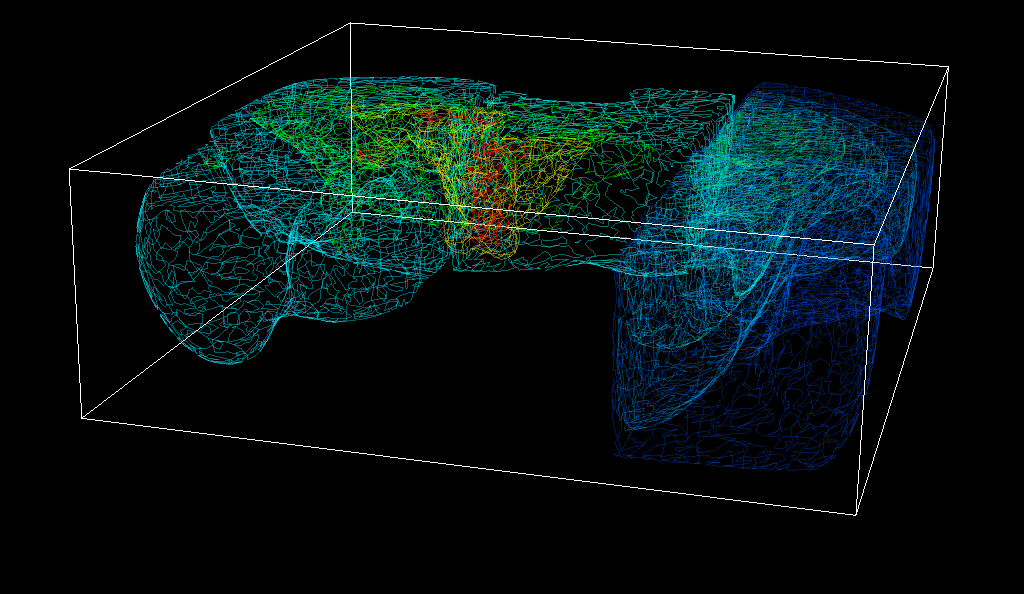
\includegraphics[width=0.8\linewidth]{images/sw4_vis_2.png}
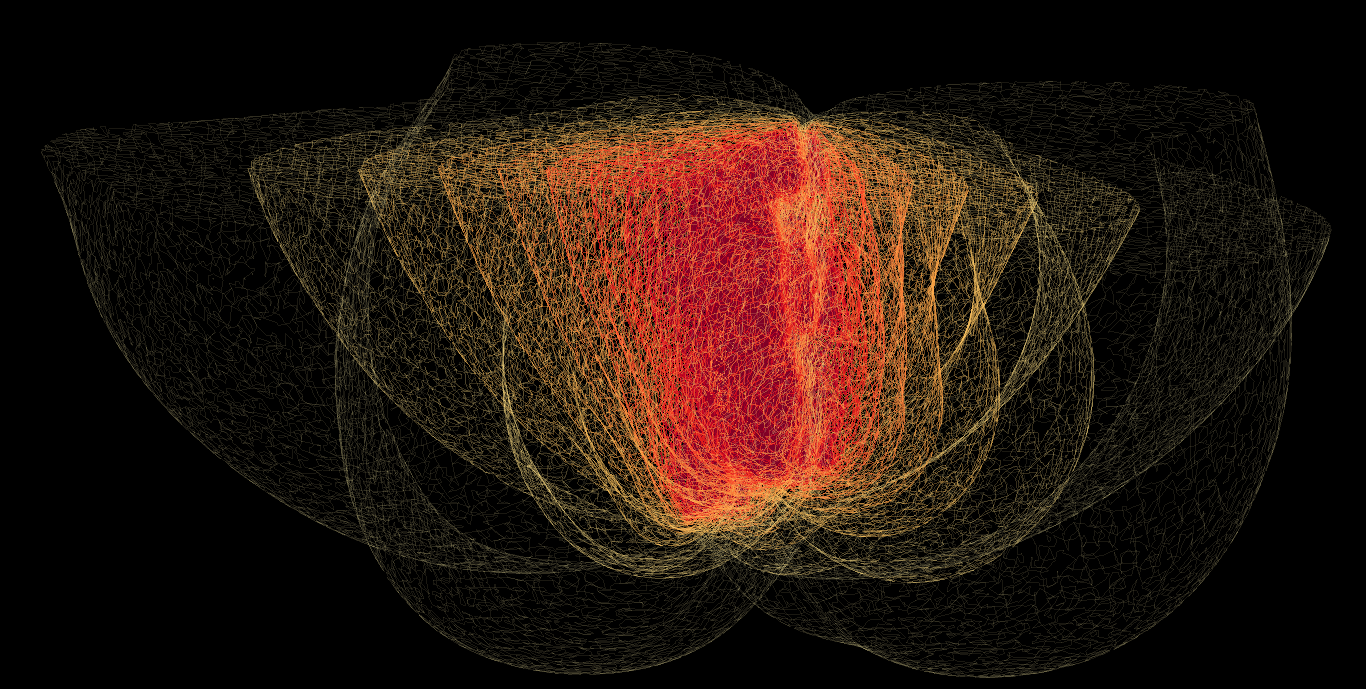
\includegraphics[width=0.8\linewidth]{images/sw4_waves.png}
\caption{SW4 wave propagation visualization}
\label{fig:sw4_vis}
\end{figure}



%\begin{figure}[t]
\centering
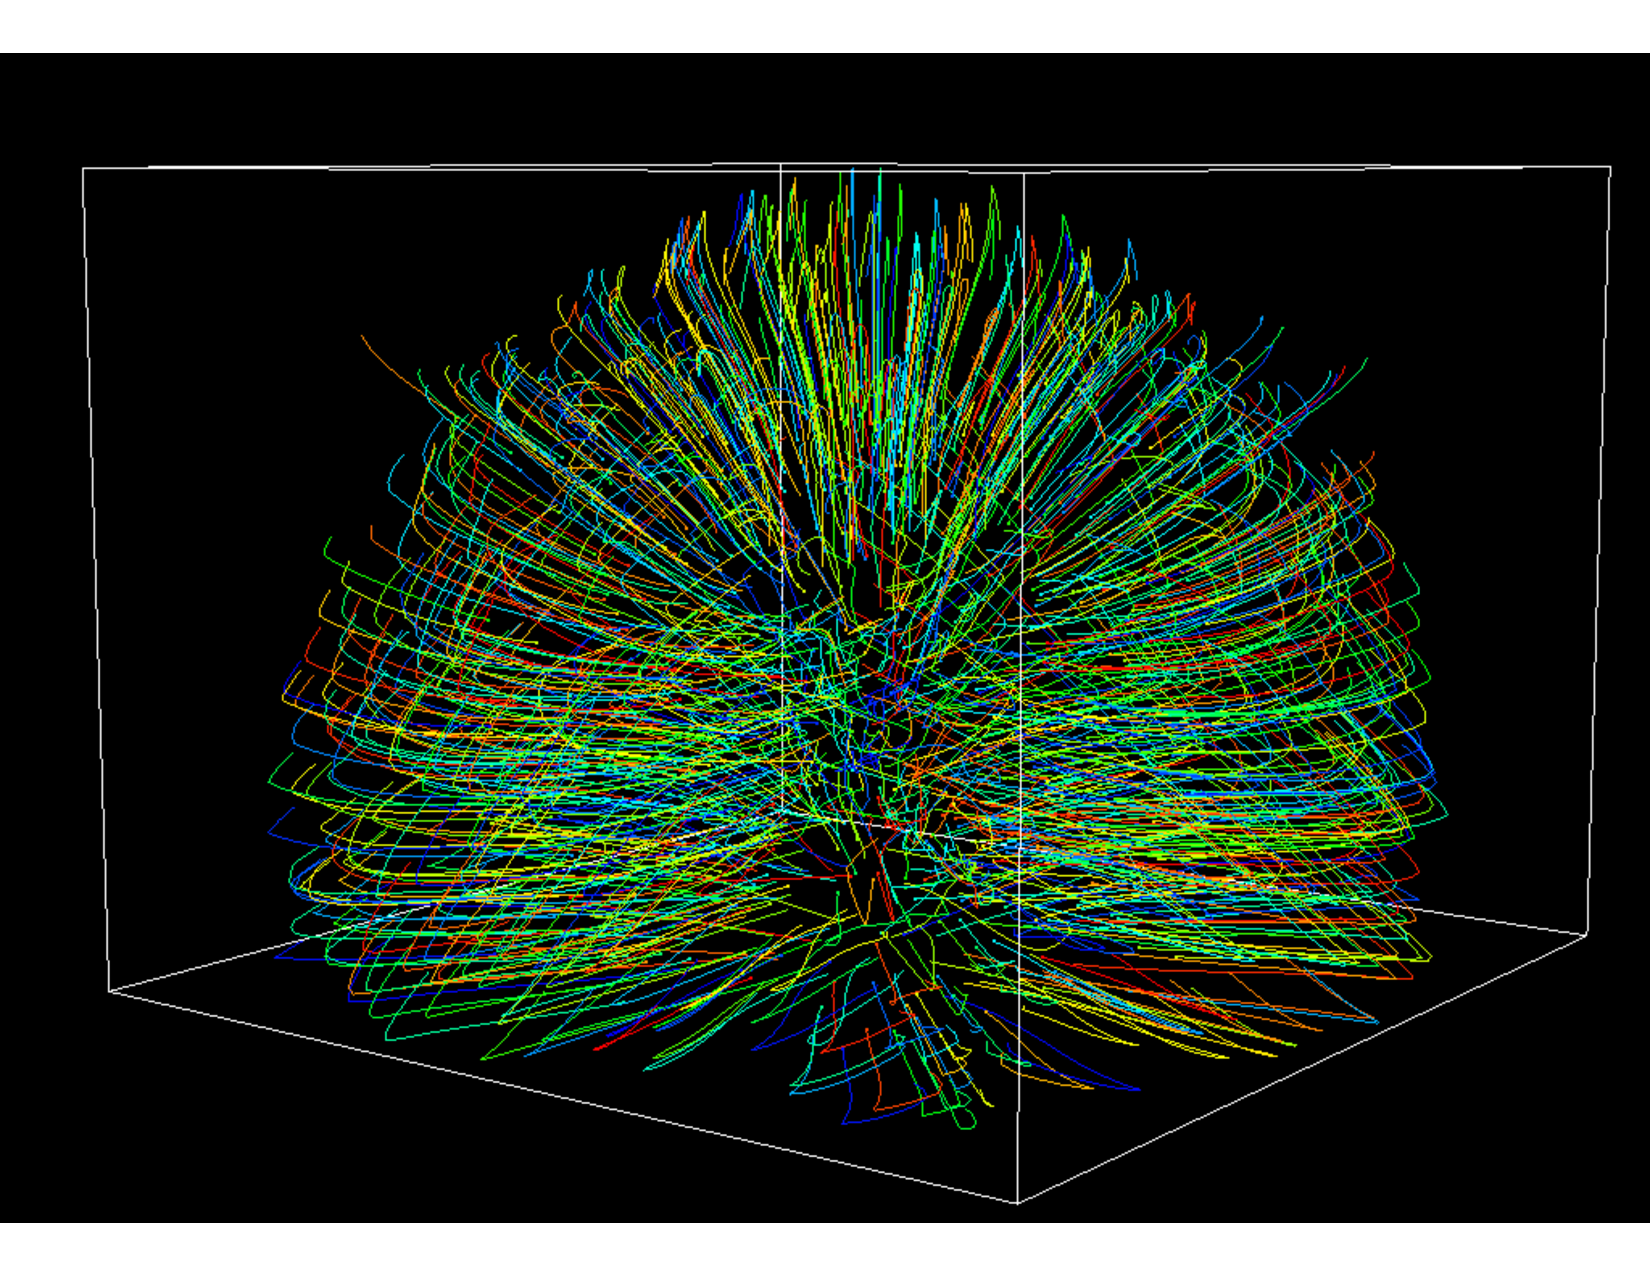
\includegraphics[width=0.7\linewidth]{images/pathlines_clover.pdf}
\caption{Cloverleaf3D flow visualization}
\label{fig:pathlines_clover}
\end{figure}



\begingroup
\setlength{\tabcolsep}{-2pt}
%\renewcommand{\arraystretch}{1} % Default value: 1
\begin{table*}[!h]
%\centering
\begin{tabular}{|P{1.1cm}|P{1.1cm}|P{2.7cm}|P{1.3cm}|P{1.3cm}|P{1.5cm}|P{2cm}  N  R|P{6cm}|}
\hline
Nodes & MPI & Dimensions & Interval & Sim$_{cycle}$ & Particles & Memory & Step & DAV\% & Scatter Plots\\ 
 & Ranks & & & & /Node & /Node (MB) & & & \\ 
\hline
%\multicolumn{9}{l}{} & \\
\multicolumn{9}{l}{\textbf{          Cloverleaf3D Proxy Hydrodynamics Application }} & \multirow{13}{*}{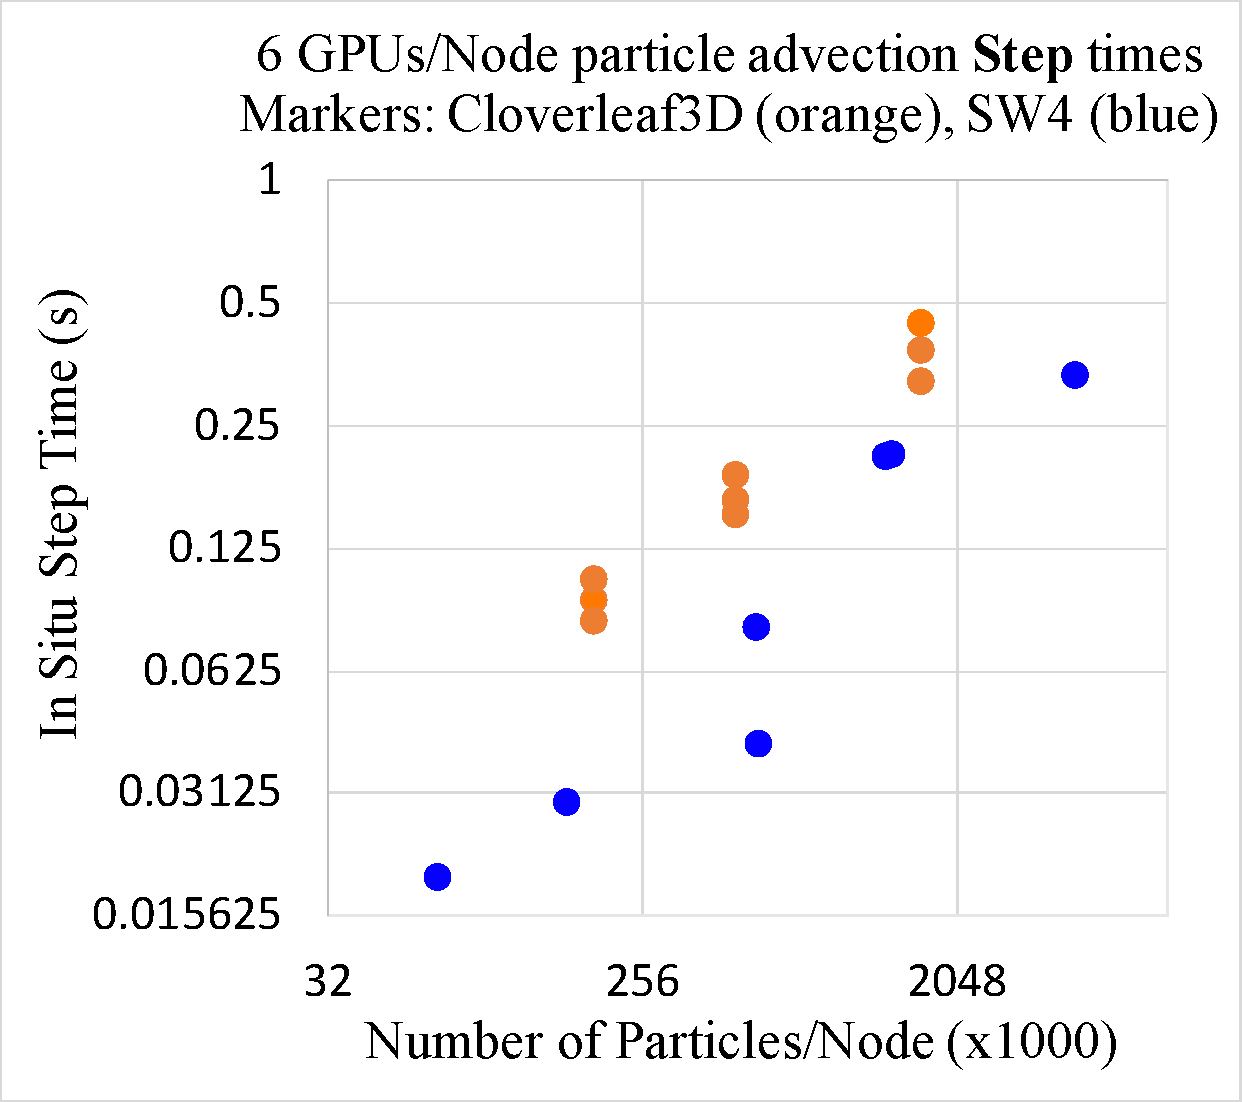
\includegraphics[width=0.93\linewidth]{images/GPU_Step.pdf}}\\
\cline{1-9}
\multirow{9}{*}{16} & \multirow{9}{*}{96} & \multirow{9}{*}{$586\times586\times586$} & 20 & 4.73 & \multirow{3}{*}{1.5M} & \multirow{3}{*}{40.2 } & 0.4475 & 9.408 & \\
\cline{4-4}
& & & 40 & 4.08 & & & 0.3221 & 7.894 & \\
\cline{4-4}
& & & 60 & 4.39 & & & 0.3838 & 8.742 & \\
\cline{4-6}%\cline{6-6}
& & & 20 & 4.50 & \multirow{3}{*}{474k} & \multirow{3}{*}{12 } & 0.1882 & 4.182 & \\
\cline{4-4}
& & & 40 & 4.14 & & & 0.1628 & 3.932 & \\
\cline{4-4}
& & & 60 & 4.33 & & & 0.1498 & 3.459 & \\
\cline{4-6}%\cline{6-6}
& & & 20 & 4.19 & \multirow{3}{*}{186k} & \multirow{3}{*}{4.2 } & 0.0925 & 2.207 & \\
\cline{4-4}
& & & 40 & 4.11 & & & 0.1043 & 2.537 & \\
\cline{4-4}
& & & 60 & 3.87 & & & 0.0830 & 2.144 & \\
\cline{1-9}
%\multicolumn{9}{l}{} & \\
\multicolumn{9}{l}{\textbf{          SW4 Seismic Modeling Simulation }} & \\
\cline{1-9}
\multirow{3}{*}{1} & \multirow{3}{*}{6} & $251\times251\times70$ & \multirow{7}{*}{200} & 0.35 & 555k & 13.89 & 0.0412 & 11.67 & \\
\cline{3-3}\cline{5-6}
& & $335\times335\times93$ & & 2.02 & 1.3M & 33.16 & 0.2125 & 10.48 & \\
\cline{3-3}\cline{5-6}  
& & $501\times501\times139$ & & 7.58 & 4.4M & 111.13 & 0.3309 & 4.365 & \multirow{13}{*}{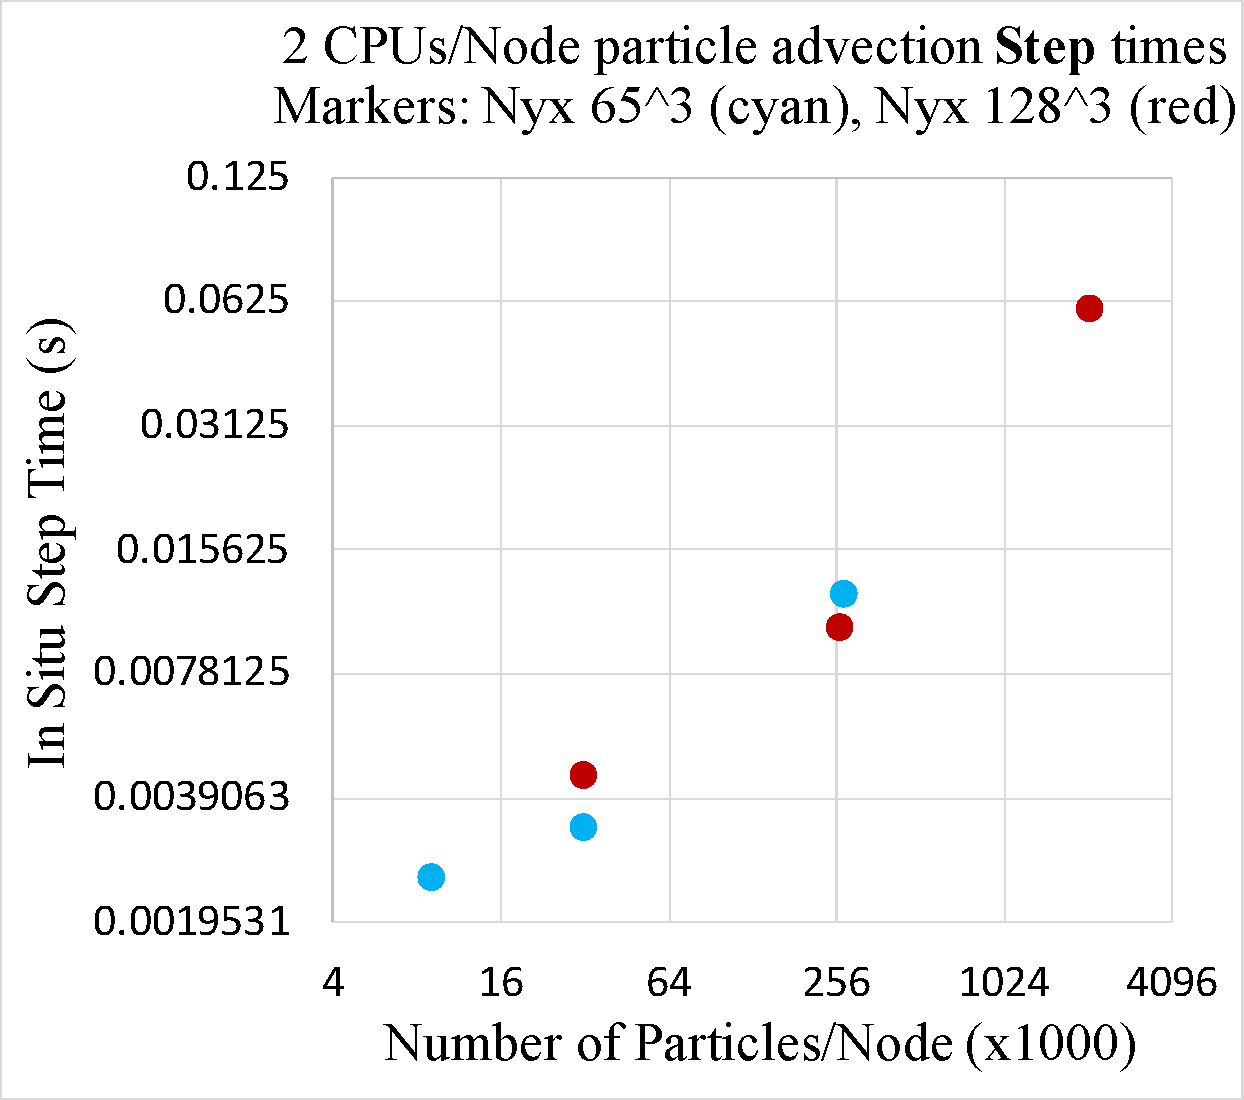
\includegraphics[width=0.93\linewidth]{images/CPU_Step.pdf}}\\
\cline{1-3}\cline{5-6}
\multirow{4}{*}{64} & \multirow{4}{*}{384} & \multirow{3}{*}{$1001\times1001\times276$} & & 1.6 & 66k & 1.6 & 0.0194 & 1.201 &  \\
\cline{6-6}
& & & & 1.5 & 146k & 3.6 & 0.0295 & 1.944 & \\
\cline{6-6}
& & & & 1.3 & 540k & 13.5 & 0.0798 & 6.175 & \\
\cline{3-3}\cline{5-6}
& & $1335\times1335\times368$ & & 2.9 & 1.2M & 31.9 & 0.2095 & 7.074 & \\
\cline{1-9}
%\multicolumn{9}{l}{} & \\
\multicolumn{9}{l}{\textbf{          Nyx Cosmology Simulation }} & \\
\cline{1-9}
\multirow{6}{*}{1} & \multirow{6}{*}{1} & \multirow{3}{*}{$65\times65\times65$} & \multirow{6}{*}{100} & \multirow{3}{*}{10.9} & 274k & 6.8 & 0.0122 & 0.112 & \\
\cline{6-6}
& & & & & 32k & 0.8 & 0.0033 & 0.030 & \\
\cline{6-6}
& & & & & 9k & 0.2 & 0.0025 & 0.023 & \\
\cline{3-3}\cline{5-6}
& & \multirow{3}{*}{$129\times129\times129$} & & \multirow{3}{*}{88.3} & 2.1M & 53.6 & 0.0596 & 0.067 & \\
\cline{6-6}
& & & & & 262k & 6.5 & 0.0101 & 0.011 & \\
\cline{6-6}
& & & & & 32k & 0.8 & 0.0044 & 0.005 & \\
\hline
\end{tabular}
\vspace{-3mm}
\caption{\textit{In situ} encumbrance evaluation and experiment configurations for our three simulation codes.}
\label{table:encumbrance}
\vspace{-5mm}
\end{table*}
\endgroup


\subsection{In Situ Encumbrance}
\label{sec:results_insitu}
%\begin{figure*}
\begin{subfigure}{0.195\textwidth}
\centering
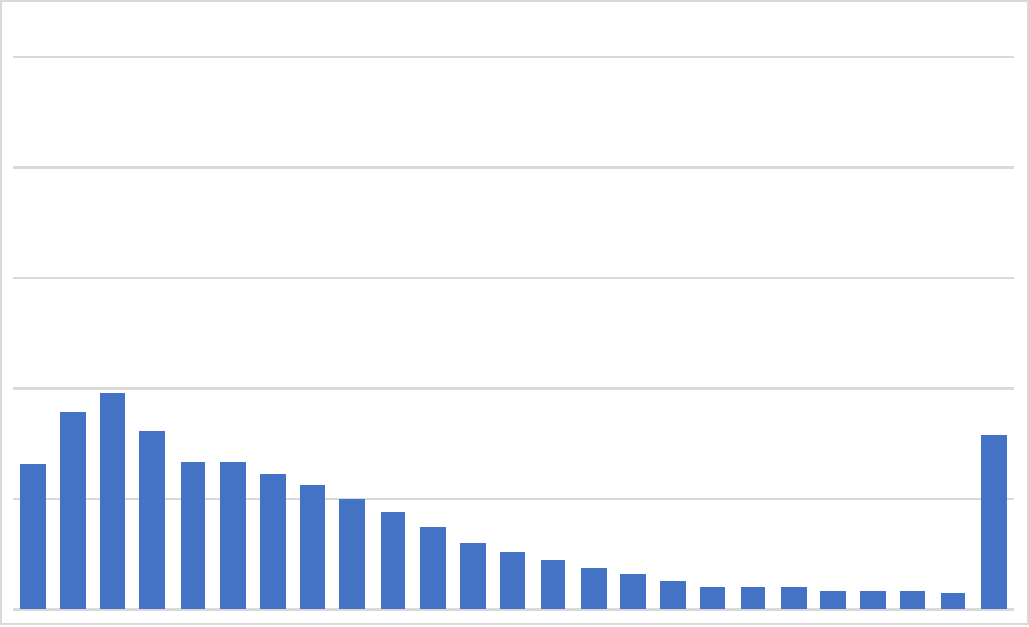
\includegraphics[width=0.9\linewidth]{results/cloverleaf3d/eul_1/Eul1_AvgL2.pdf}
\vspace{-2mm}
\caption{Eul 20 Avg$_{L2}$ L2 }
\end{subfigure}
\begin{subfigure}{0.195\textwidth}
\centering
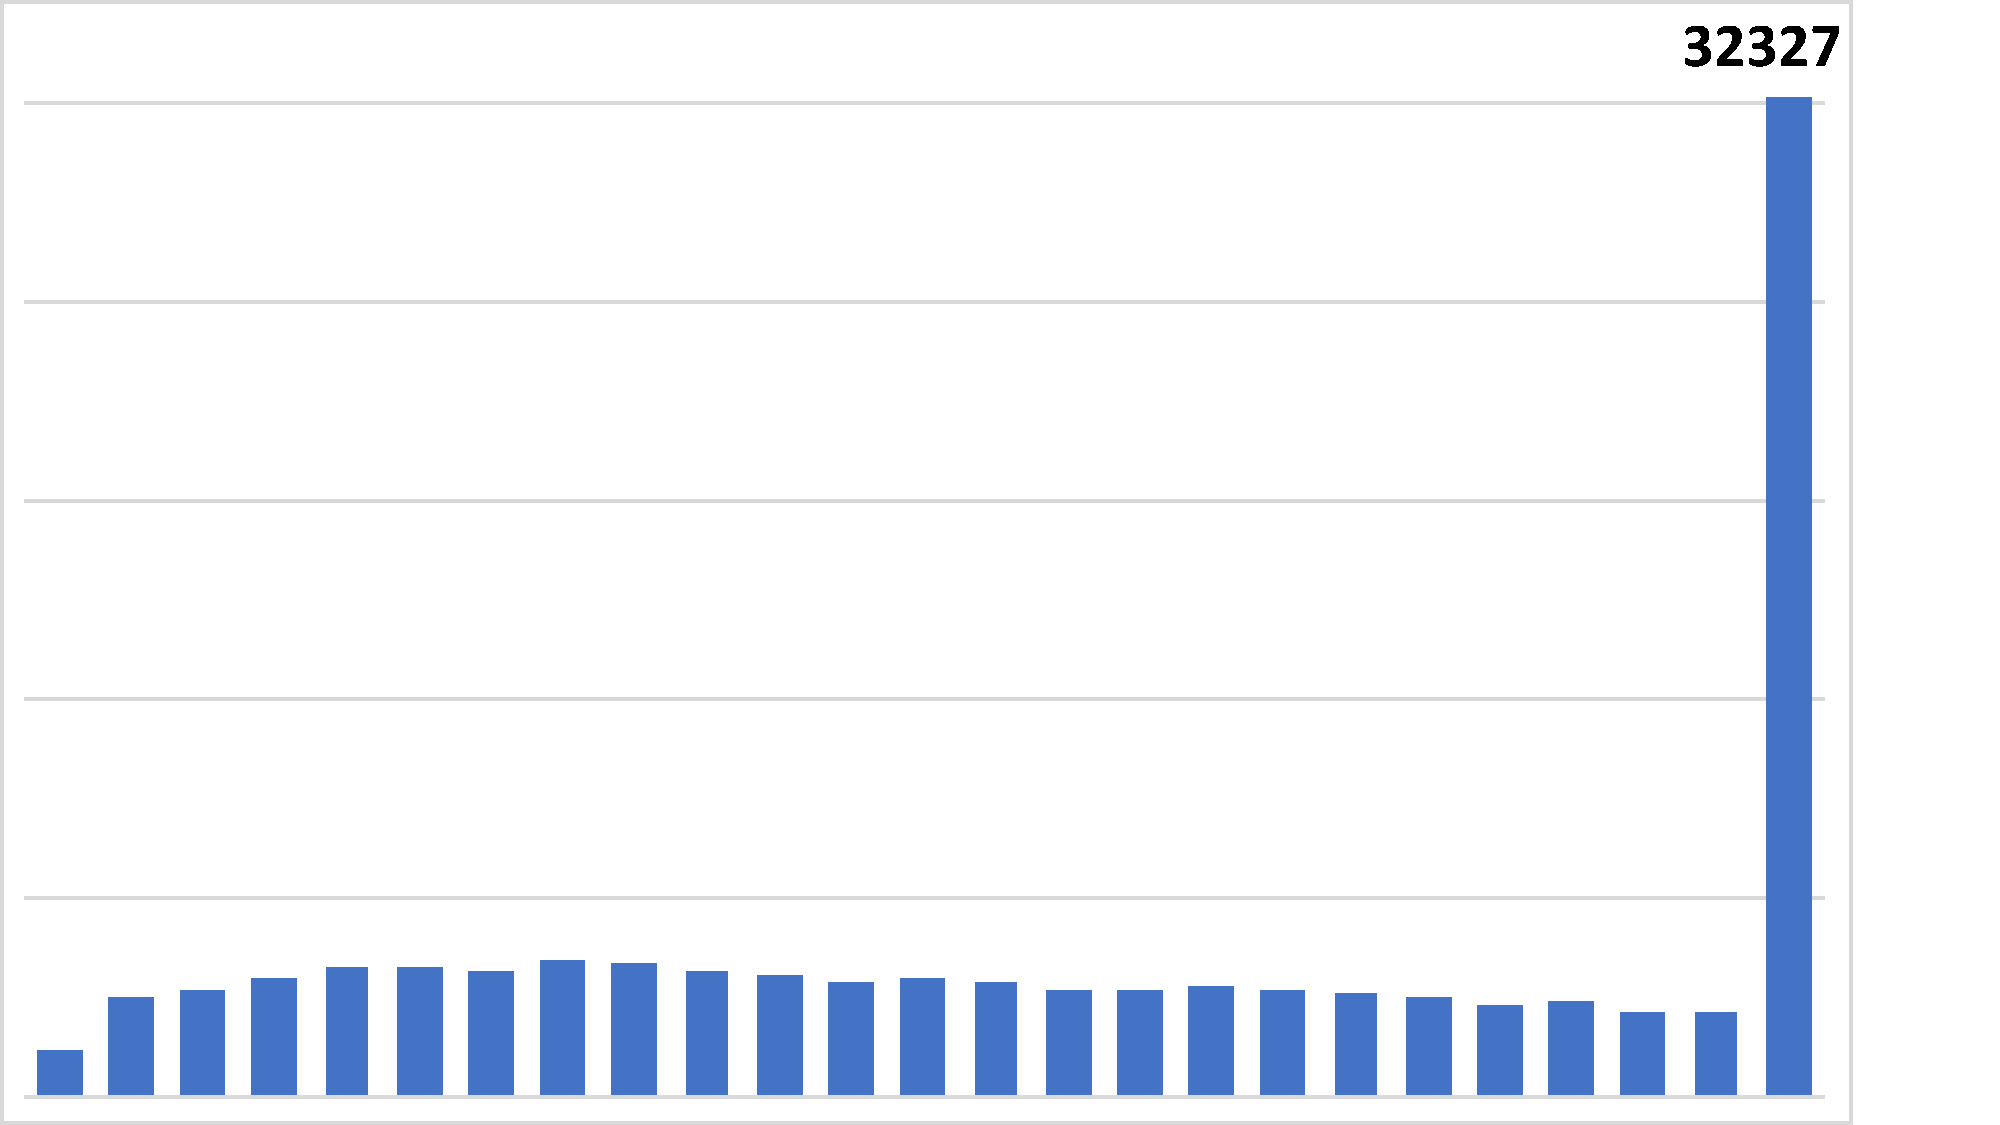
\includegraphics[width=0.95\linewidth]{results/cloverleaf3d/eul_2/Eul2_AvgL2.pdf}
\vspace{-2mm}
\caption{Eul 40 Avg$_{L2}$ L2 }
\end{subfigure}
\begin{subfigure}{0.195\textwidth}
\centering
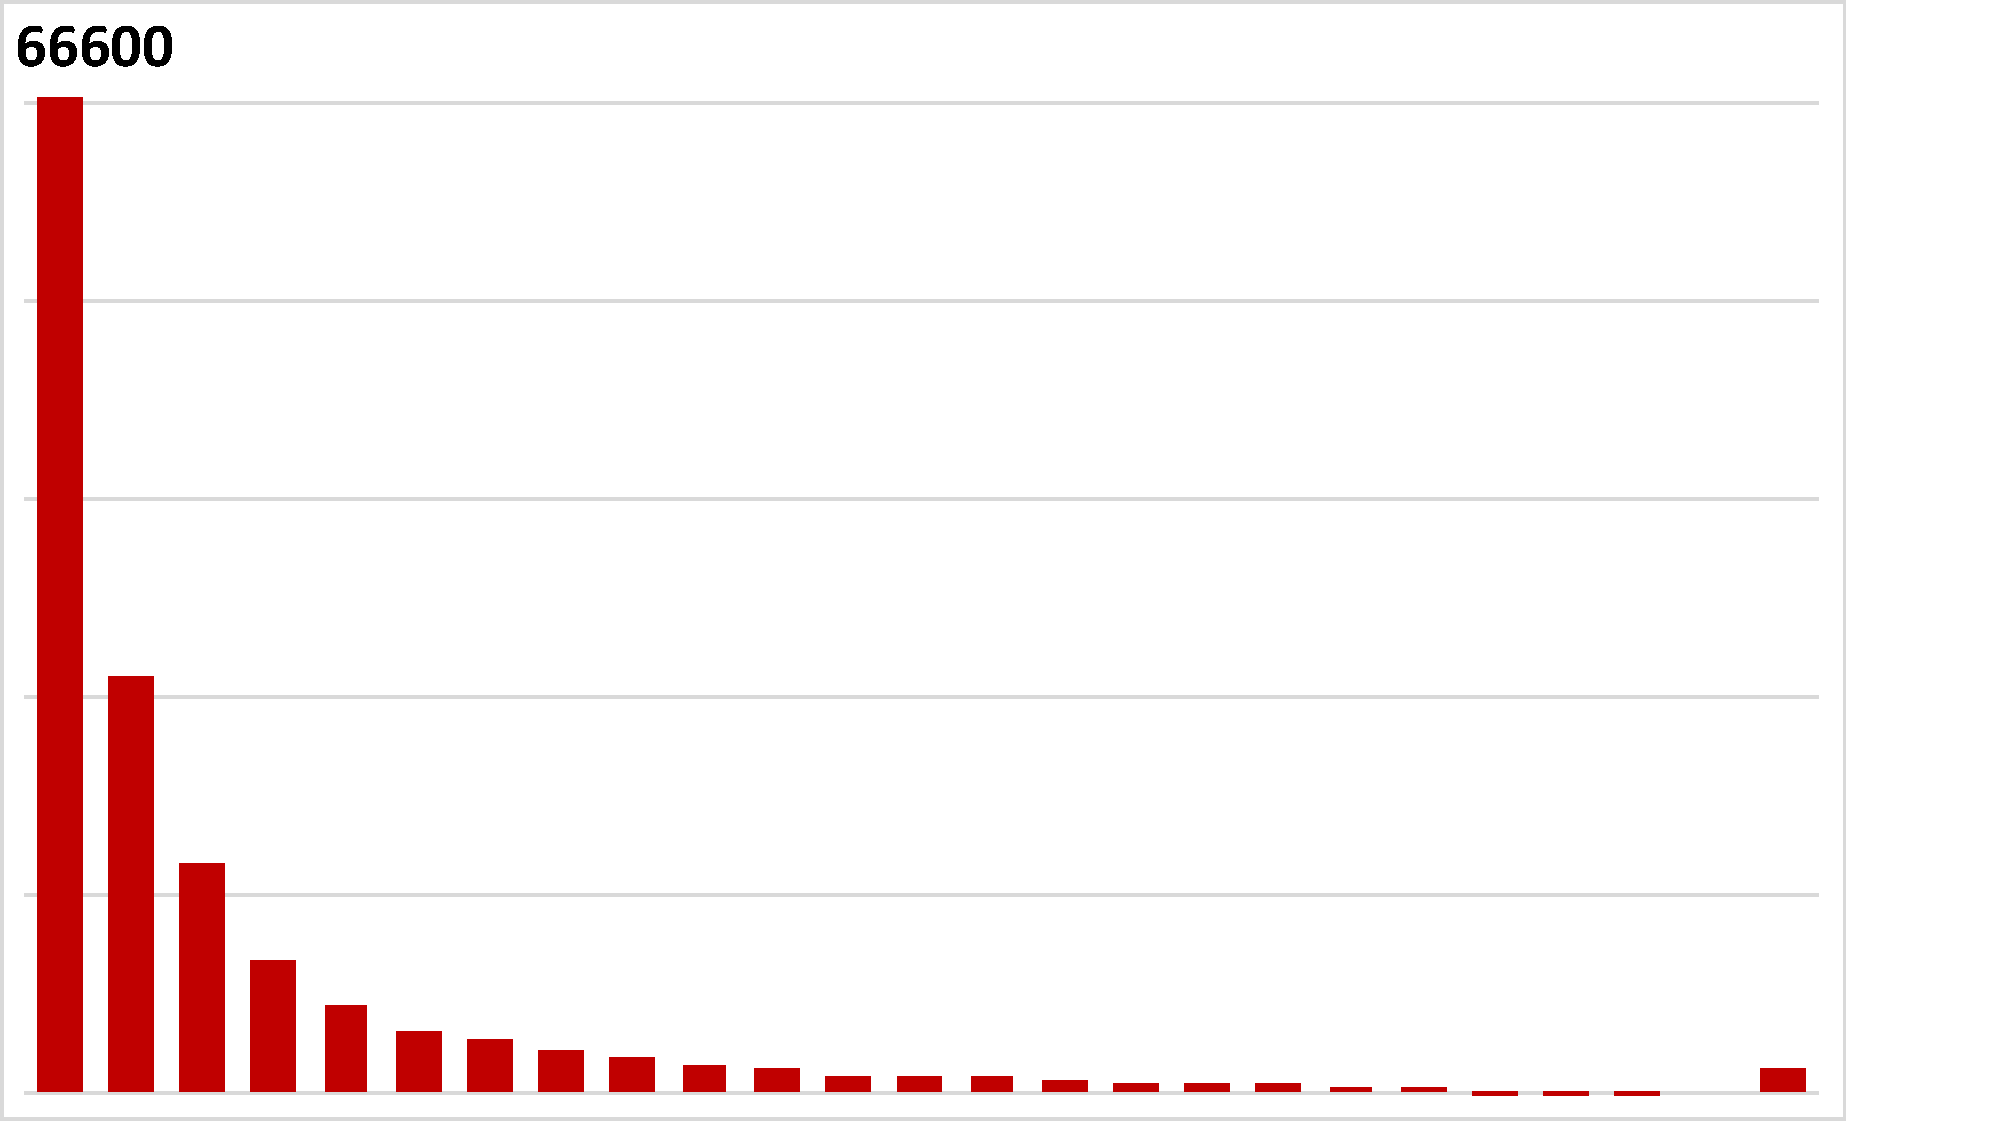
\includegraphics[width=0.9\linewidth, trim={0cm 0cm 2.5cm 0cm}, clip]{results/cloverleaf3d/lag_4/Lag4_AvgL2.pdf}
\vspace{-2mm}
\caption{Lag 40 1:8 Avg$_{L2}$ }
\end{subfigure}
\begin{subfigure}{0.195\textwidth}
\centering
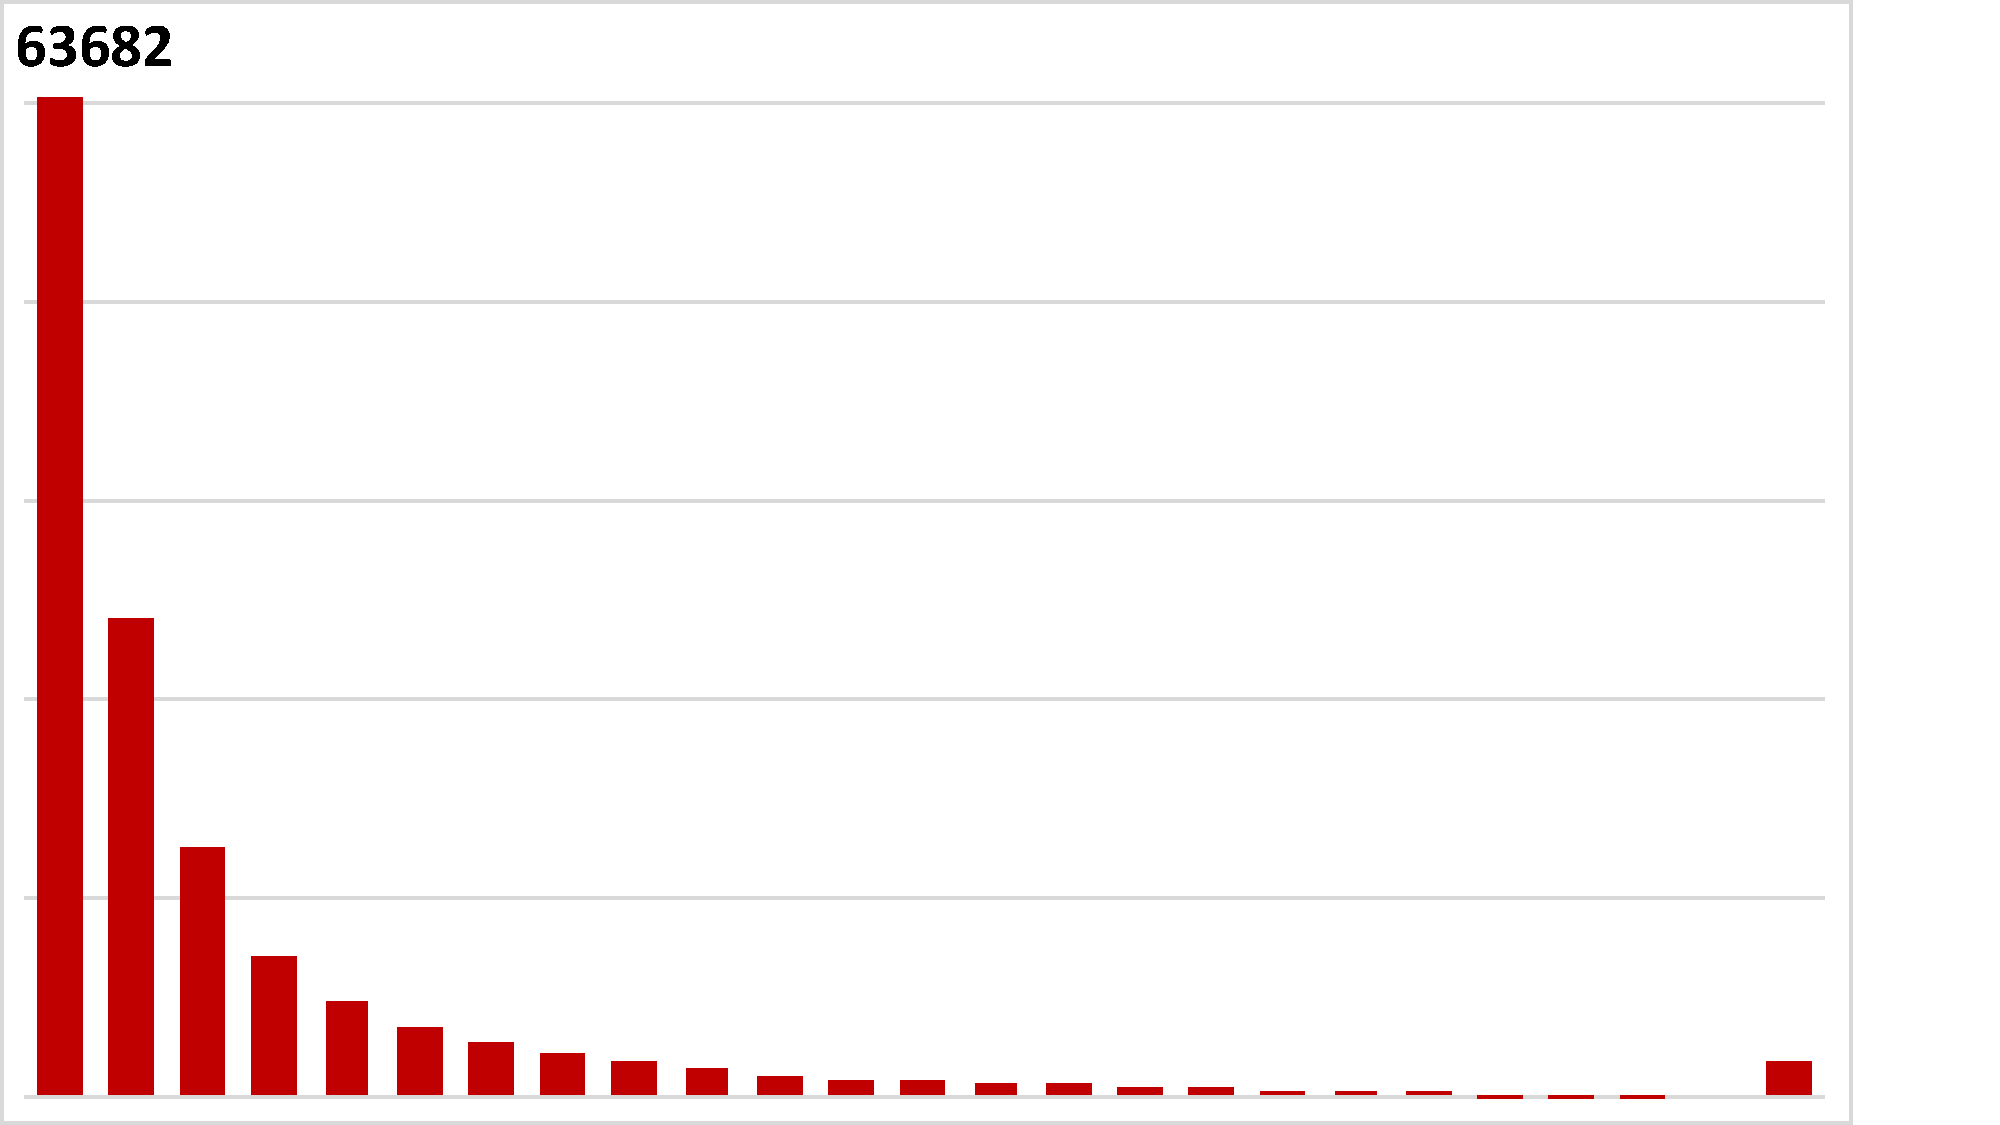
\includegraphics[width=0.9\linewidth, trim={0cm 0cm 2.5cm 0cm}, clip]{results/cloverleaf3d/lag_5/Lag5_AvgL2.pdf}
\vspace{-2mm}
\caption{Lag 40 1:27 Avg$_{L2}$ }
\end{subfigure}
\begin{subfigure}{0.195\textwidth}
\centering
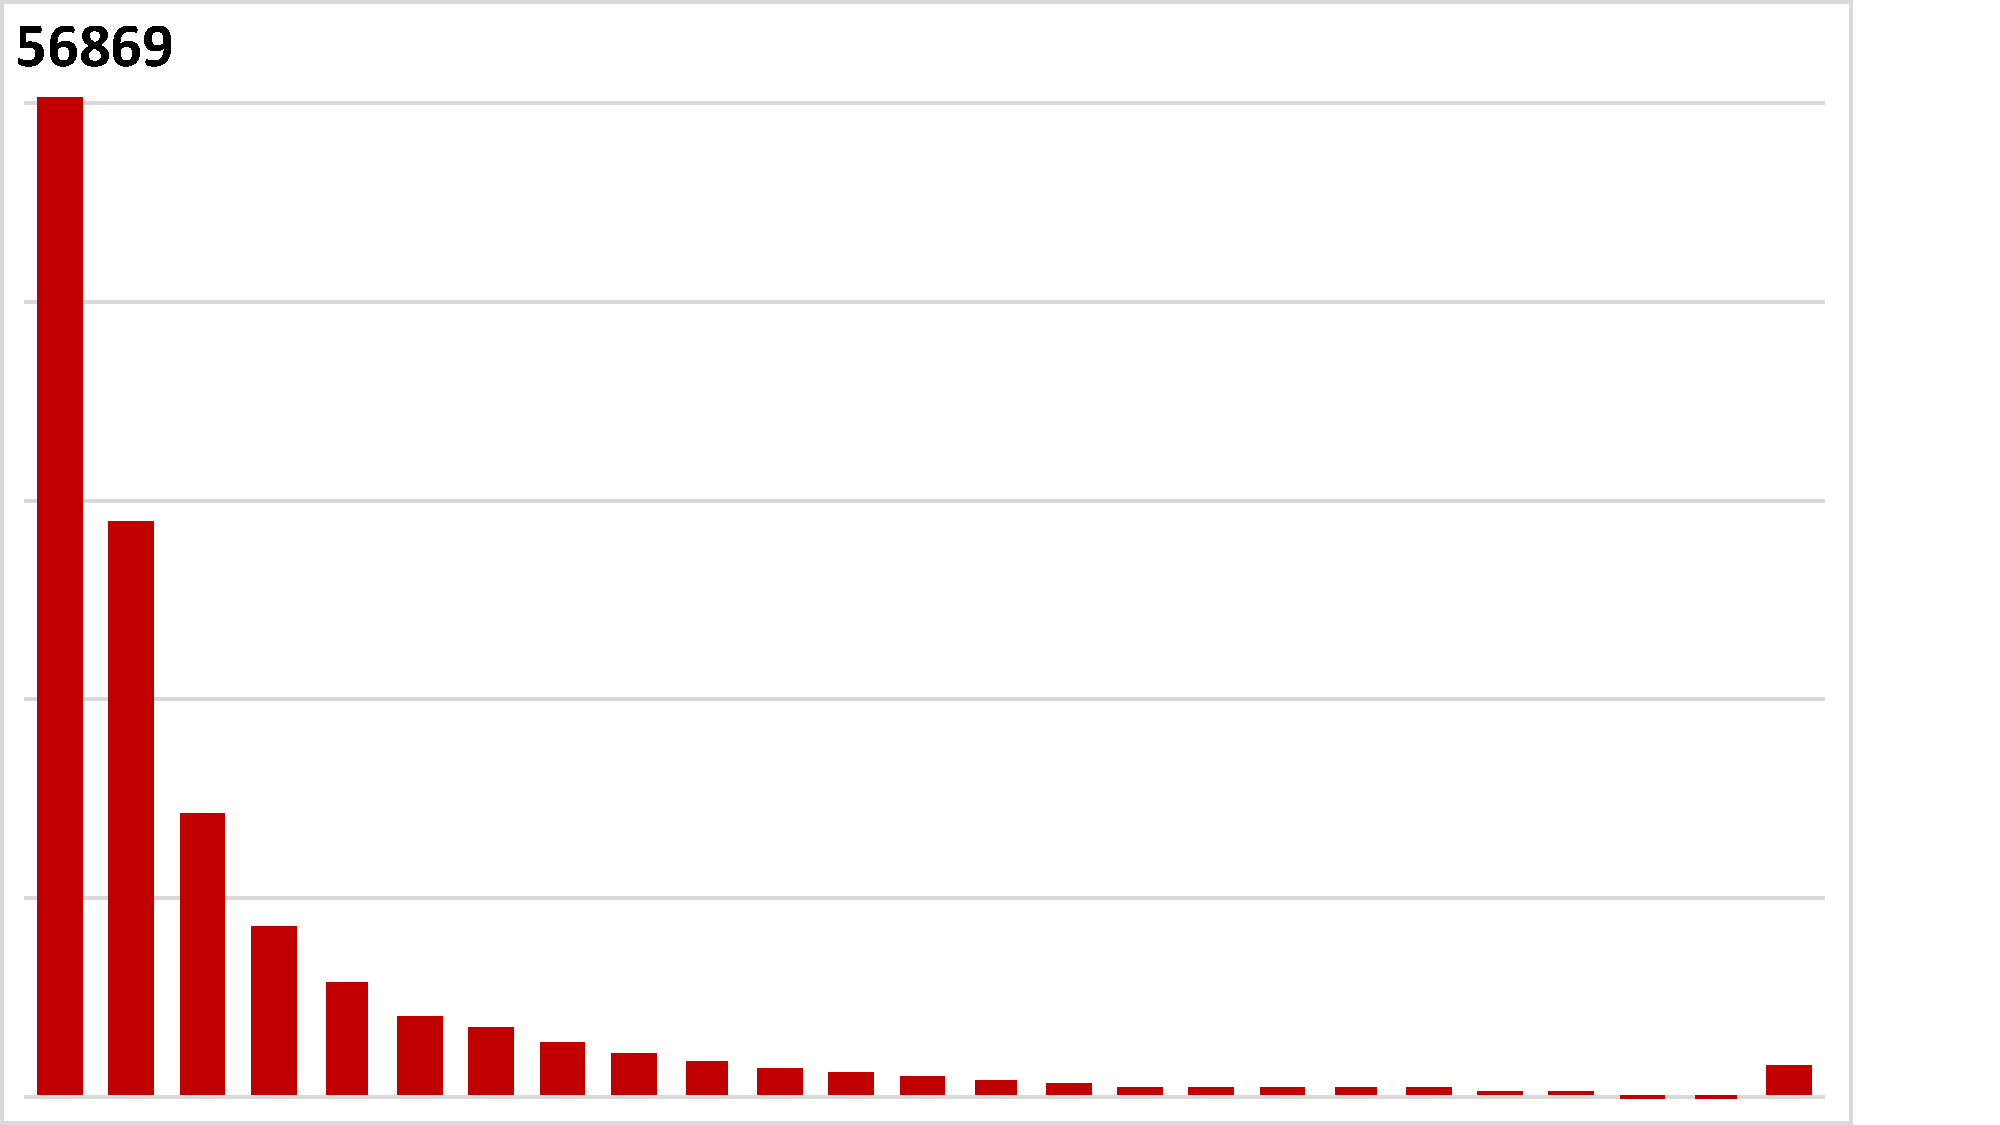
\includegraphics[width=0.9\linewidth, trim={0cm 0cm 2.5cm 0cm}, clip]{results/cloverleaf3d/lag_6/Lag6_AvgL2.pdf}
\vspace{-2mm}
\caption{Lag 40 1:64 Avg$_{L2}$ }
\end{subfigure}
\begin{subfigure}{0.195\textwidth}
\centering
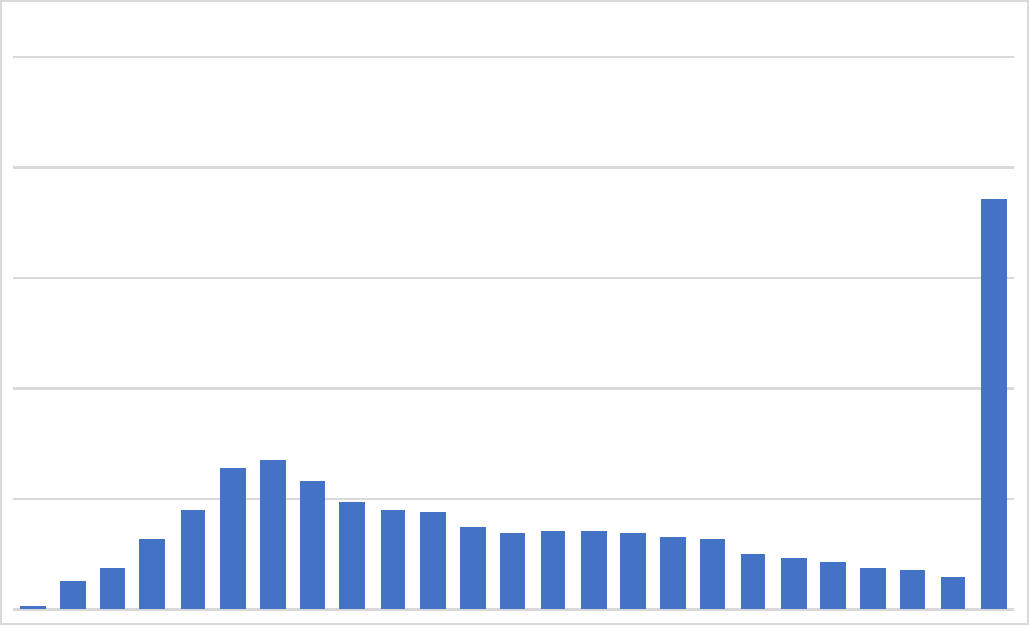
\includegraphics[width=0.9\linewidth]{results/cloverleaf3d/eul_1/Eul1_Max.pdf}
\vspace{-2mm}
\caption{Eul 20 Max$_{L2}$ }
\end{subfigure}
\begin{subfigure}{0.195\textwidth}
\centering
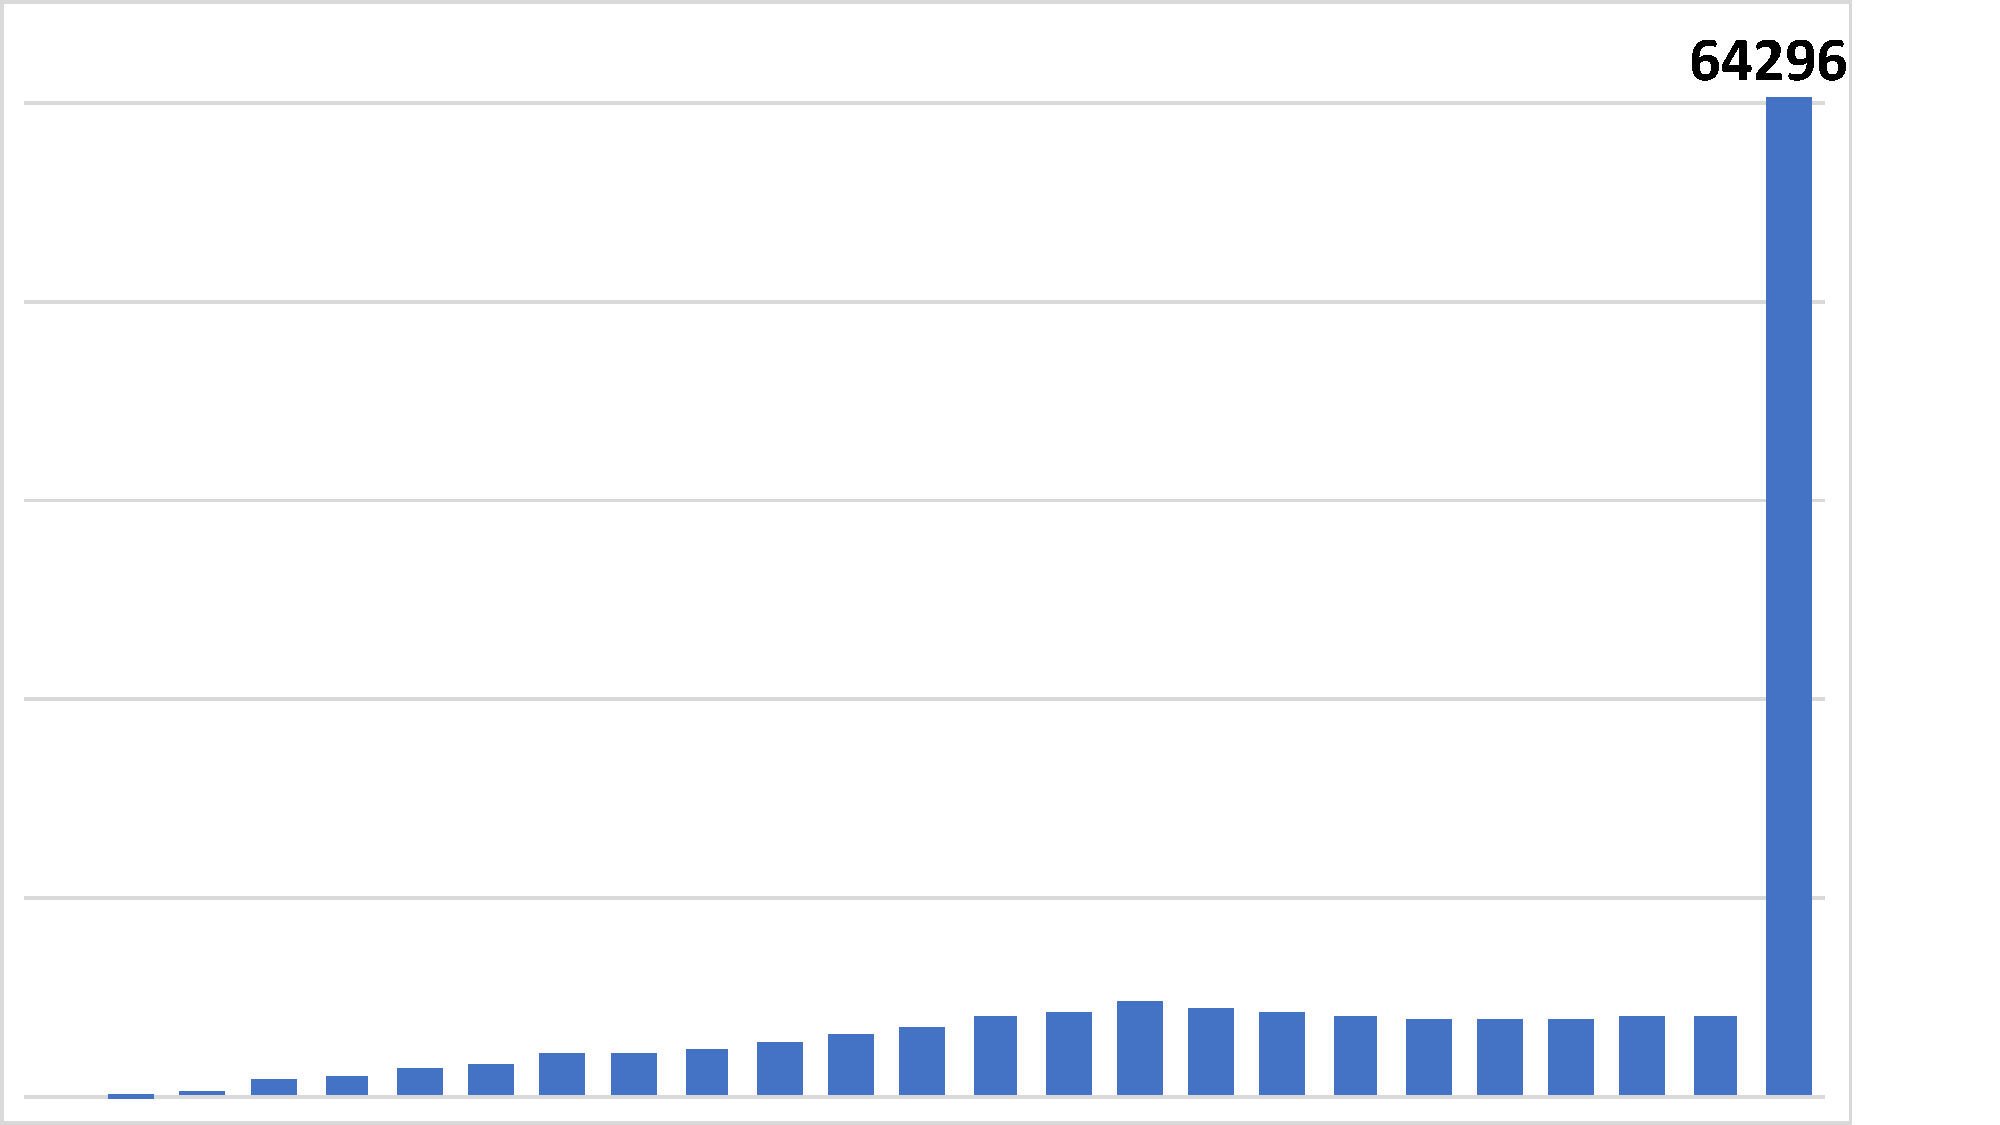
\includegraphics[width=0.95\linewidth]{results/cloverleaf3d/eul_2/Eul2_Max.pdf}
\vspace{-2mm}
\caption{Eul 40 Max$_{L2}$ }
\end{subfigure}
\hspace{0.2mm}
\begin{subfigure}{0.195\textwidth}
\centering
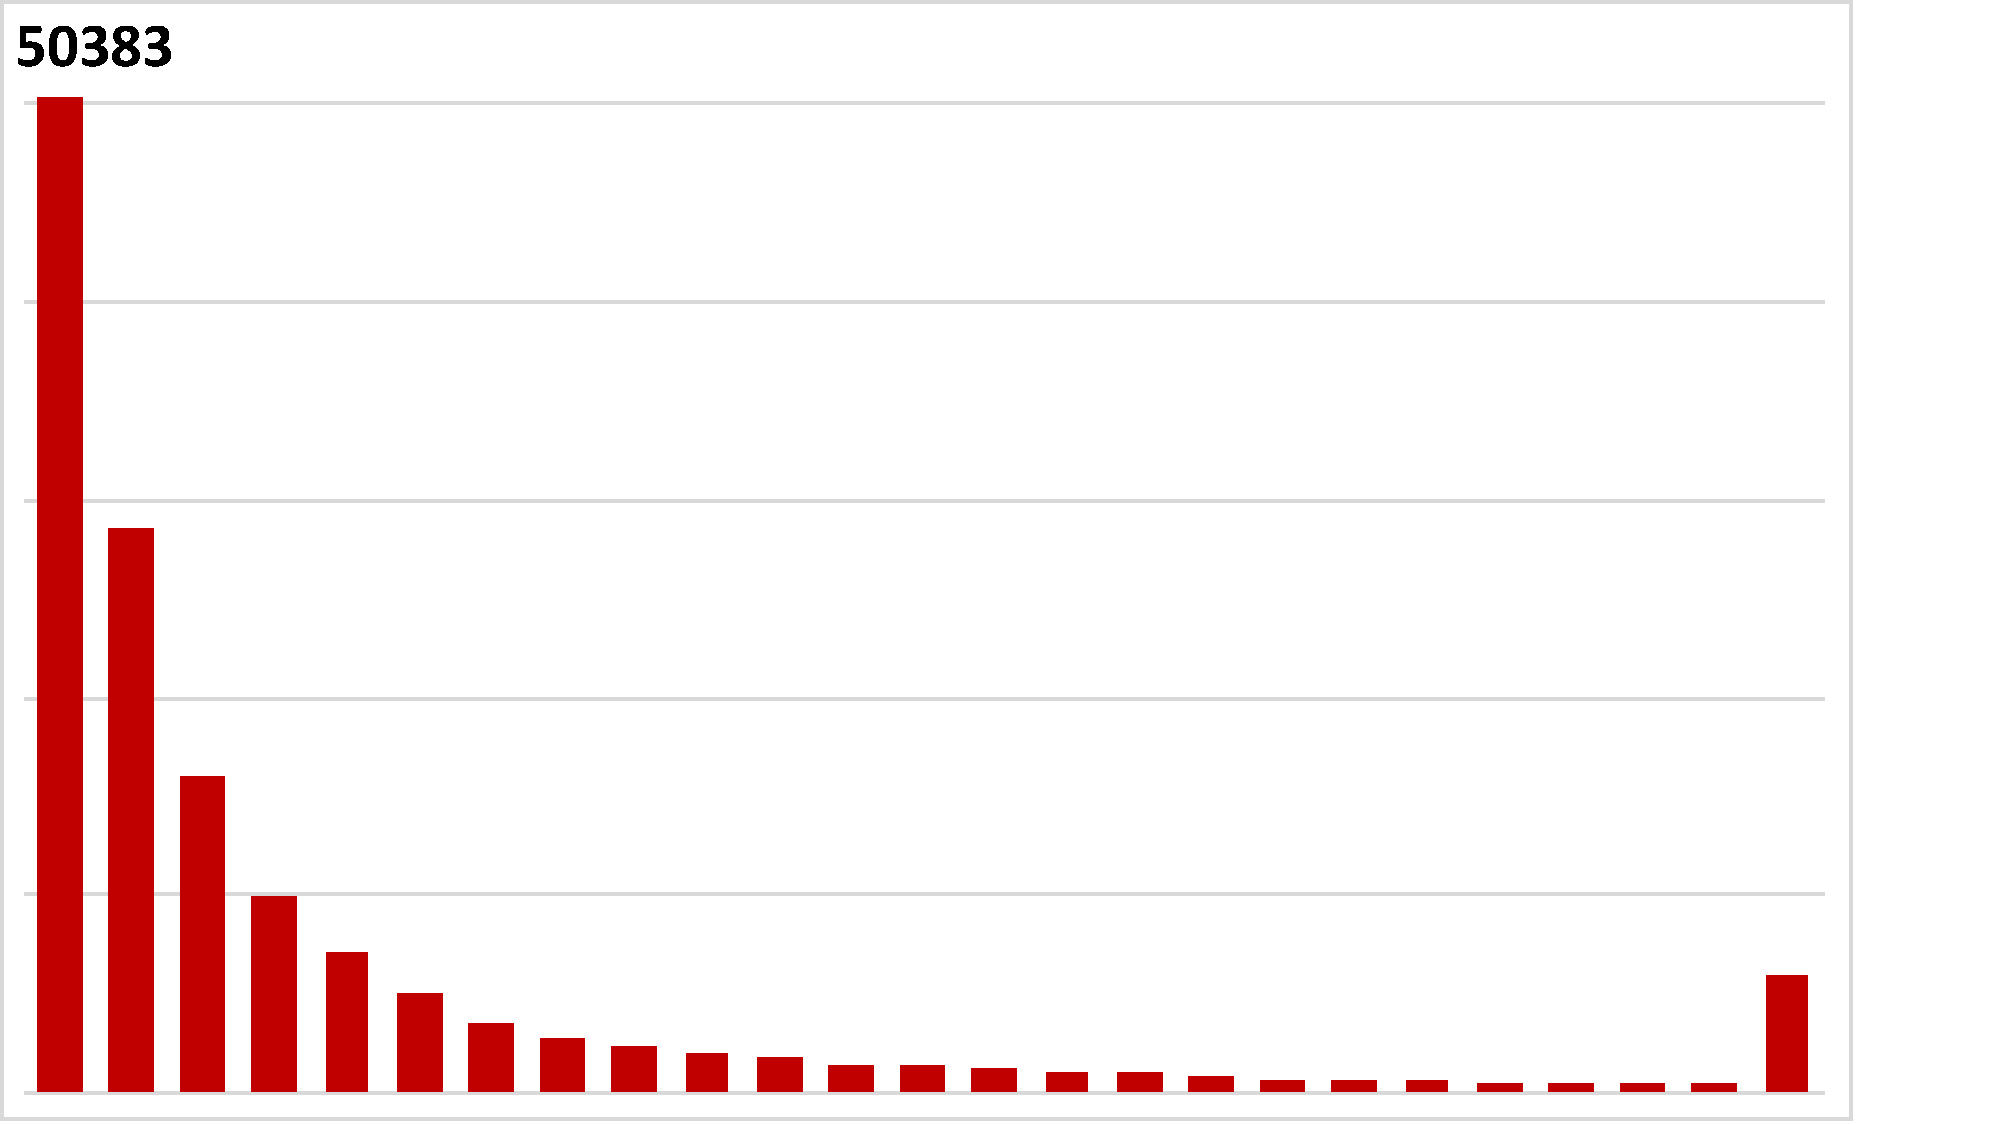
\includegraphics[width=0.9\linewidth, trim={0cm 0cm 2.5cm 0cm}, clip]{results/cloverleaf3d/lag_4/Lag4_Max.pdf}
\vspace{-2mm}
\caption{Lag 40 1:8 Max$_{L2}$ }
\end{subfigure}
\begin{subfigure}{0.195\textwidth}
\centering
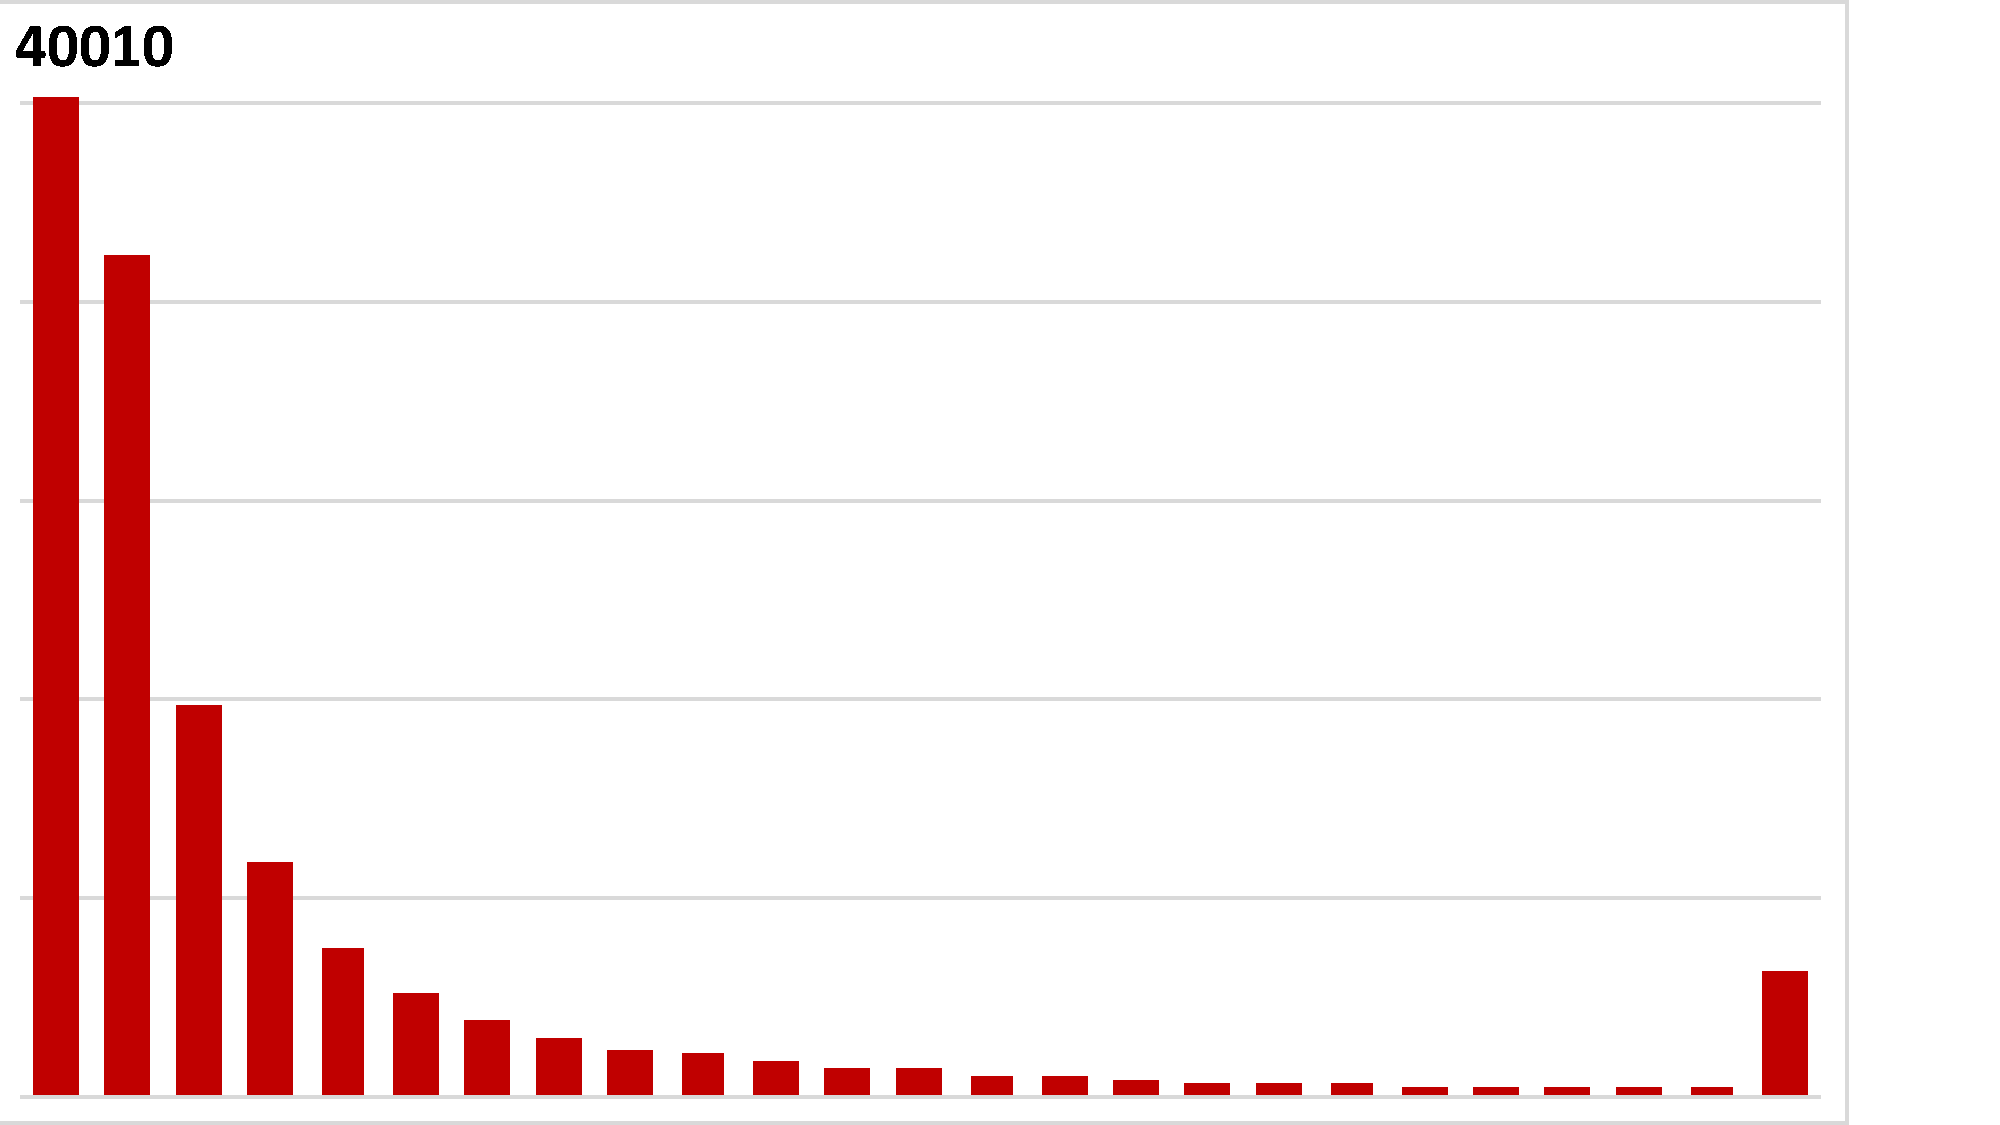
\includegraphics[width=0.9\linewidth, trim={0cm 0cm 2.5cm 0cm}, clip]{results/cloverleaf3d/lag_5/Lag5_Max.pdf}
\vspace{-2mm}
\caption{Lag 40 1:27 Max$_{L2}$}
\end{subfigure}
\begin{subfigure}{0.195\textwidth}
\centering
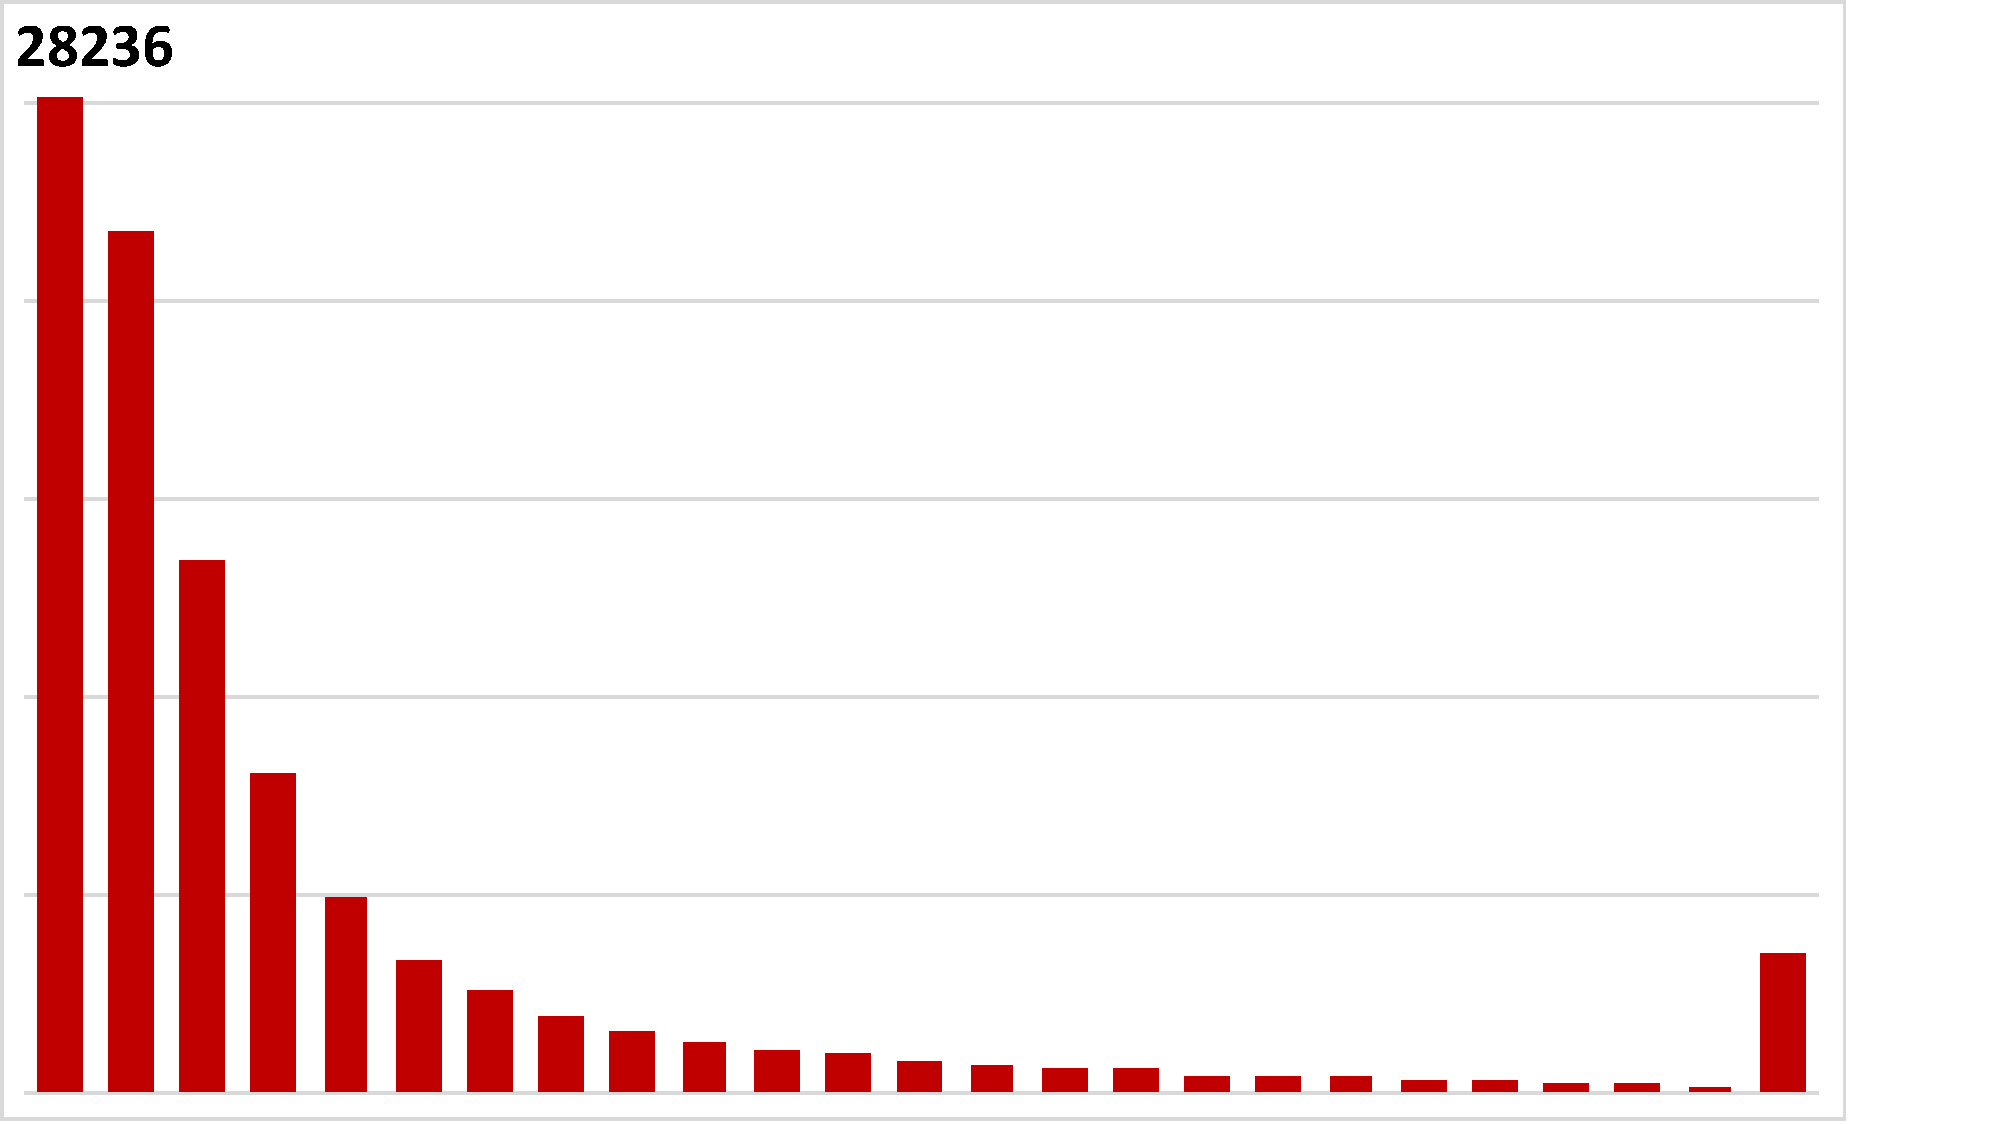
\includegraphics[width=0.9\linewidth, trim={0cm 0cm 2.5cm 0cm}, clip]{results/cloverleaf3d/lag_6/Lag6_Max.pdf}
\vspace{-2mm}
\caption{Lag 40 1:64 Max$_{L2}$}
\end{subfigure}
%\begin{subfigure}{0.24\textwidth}
%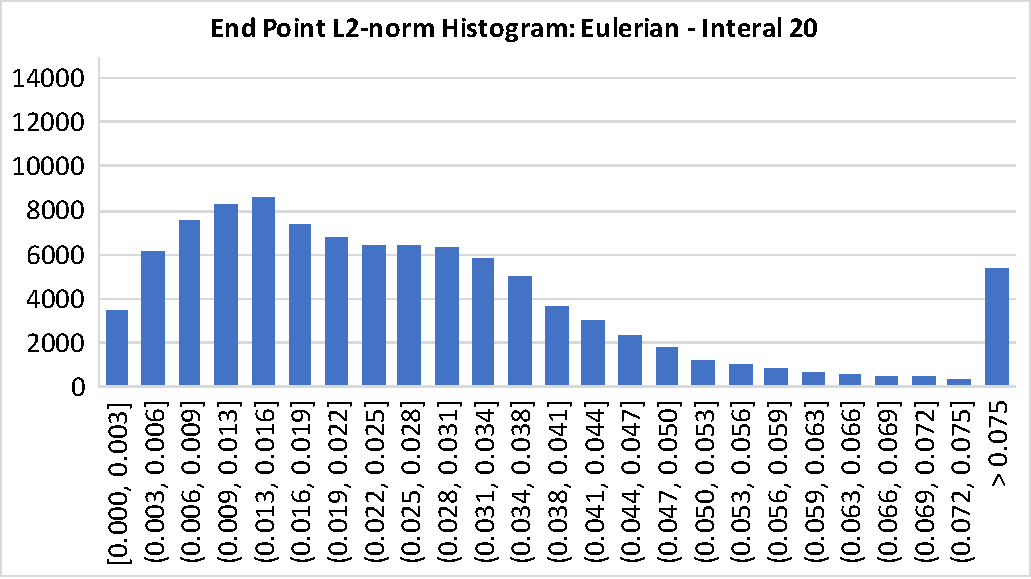
\includegraphics[width=0.9\linewidth]{results/cloverleaf3d/eul_1/Eul1_EndPt.pdf}
%\caption{Eulerian 20 End Point}
%\end{subfigure}
%\hspace{1mm}
%\begin{subfigure}{0.21\textwidth}
%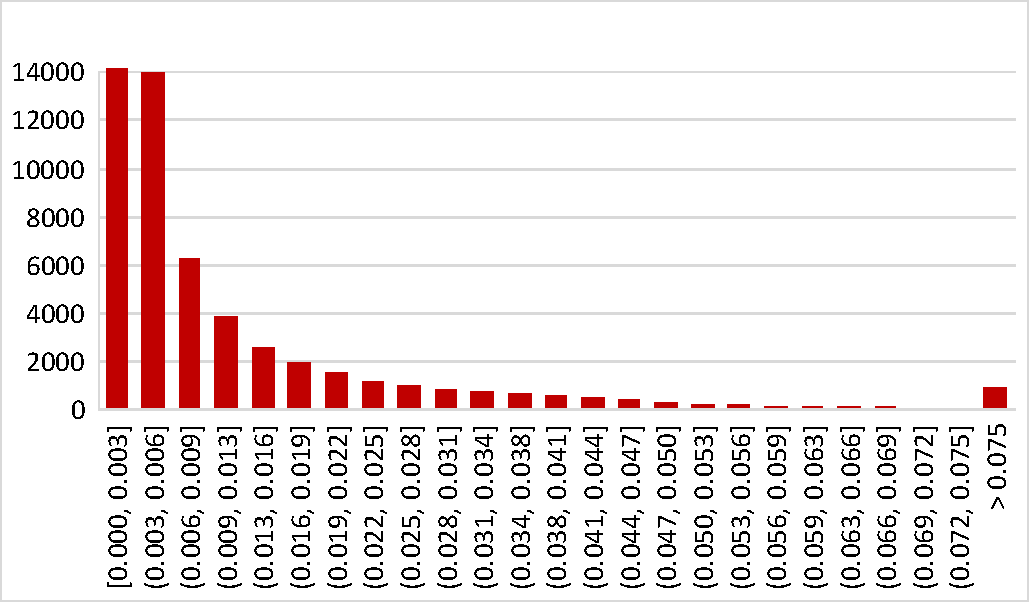
\includegraphics[width=1\linewidth]{results/cloverleaf3d/lag_4/Lag4_EndPt.pdf}
%\caption{Lagrangian 40 1:8 End Point}
%\end{subfigure}
%\hspace{1mm}
%\begin{subfigure}{0.21\textwidth}
%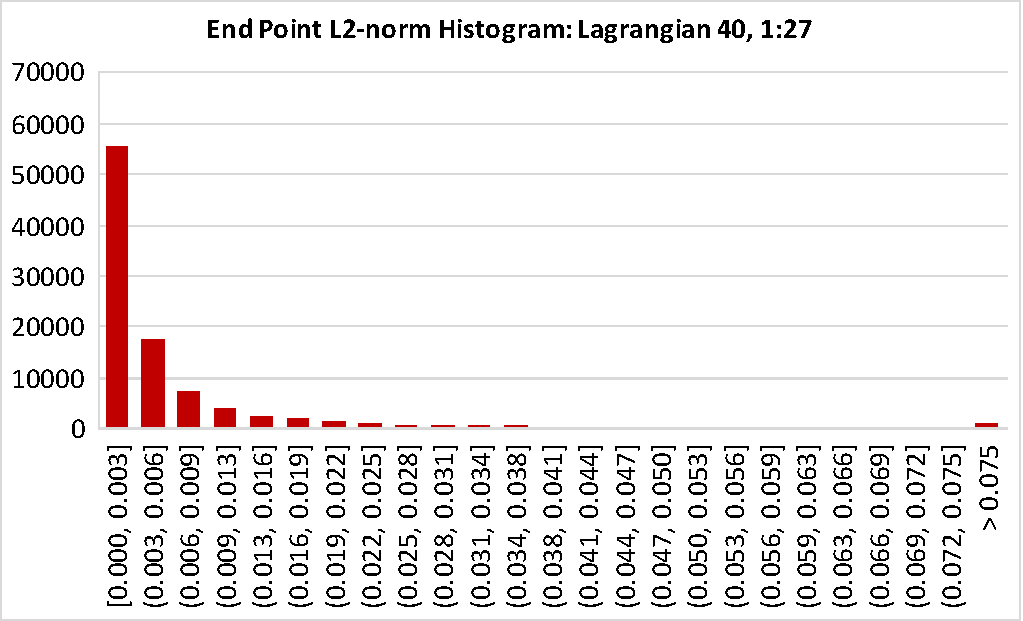
\includegraphics[width=1\linewidth]{results/cloverleaf3d/lag_5/Lag5_EndPt.pdf}
%\caption{Lagrangian 40 1:27 End Point}
%\end{subfigure}
%\hspace{1mm}
%\begin{subfigure}{0.21\textwidth}
%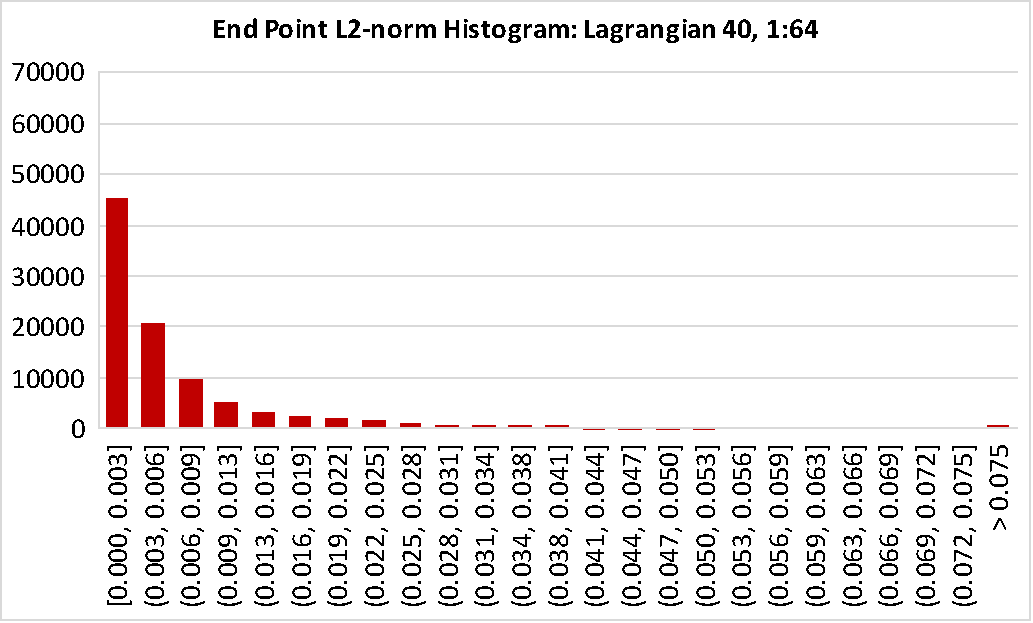
\includegraphics[width=1\linewidth]{results/cloverleaf3d/lag_6/Lag6_EndPt.pdf}
%\caption{Lagrangian 40 1:64 End Point}
%\end{subfigure}
\vspace{-3mm}
\caption{\textbf{Cloverleaf3D} experiment histograms for 100,000 test particle interpolation errors. Each plot has 25 bins, ranging from 0 to $>$0.05, with bar height encoding number of particles. Horizontal grid lines mark increments of 5,000.} 
\label{fig:clover_histograms}
\vspace{-6mm}
\end{figure*}


%\input{timings.tex}
Table~\ref{table:encumbrance} contains the results of our experiments for this campaign using all three simulation codes.
%
In this discussion, we assume a simulation can afford to spend 10\% to 20\% on \textit{in situ} processing routines and refer to this as the \textbf{budget}. 
%
Although this might not hold true for every simulation, this estimate is based on interactions with computational scientists and thus, we believe this is a reasonable working estimate.
%
The \textbf{Step} and \textbf{DAV\%} columns in Table~\ref{table:encumbrance} redundantly encode the value in each cell using cell background color (white to pure red hue for the ranges [0,0.75]~(\textbf{Step} in seconds) and [0,20]~(\textbf{DAV\%}), respectively).
%

For \textbf{ISR-2}, i.e., memory costs, we observe that across all experiments, the largest usage of runtime memory was approximately 112 MB.
%
Each Summit node has multiple GBs of memory on CPU~(512) and GPU~(16), and we believe extracting a Lagrangian representation increases the cost of memory on the simulation by approximately one simulation ``field''.
%
We note that simulations can have tens to hundreds of fields defined on the simulation grid and thus, this cost would likely be considered acceptable for most simulations.
%
Our reporting of memory usage is contained in Table~\ref{table:encumbrance}.

\subsubsection{Cloverleaf3D Hydrodynamics Proxy Simulation}
For the Cloverleaf3D simulation, we considered 3 options for number of particles and interval, and 1 option for grid size and concurrency.
%
In particular, we are interested in the \textit{in situ} encumbrance (\textbf{ISR-1}) of varying particle advection workloads, i.e., the number of particles. 
%
We note that each node used 6 GPUs for particle advection and that they all access the same shared memory.
%
For our specific grid size and domain decomposition, each MPI rank operated on over 2M grid points and the Sim$_{cycle}$ was usually between 4-5 seconds. 
%
Overall, we observe an increase in \textbf{Step} costs as the number of particles advected per node increases.
%
Given, the Sim$_{cycle}$ remained relatively stable, the increase in \textbf{Step} is clearly matched by the \textbf{DAV\%} trend.
%

For this integration, we observed that as the number of particles increases from 186k to 474k (2.5X increase) that the cost of performing particle advection only increases by approximately 1.6X. 
%
For the next workload increase, i.e., sampling 1.5M particles ($\sim$3X increase), the cost of performing particle advection increases by approximately 2X.
%
By running the same workload multiple times, we capture variation in the costs within a workload.
%
The variation in the \textbf{Step} cost is greater when the workload is larger and we attribute this to the increased memory allocation and memory transfer costs each step.
%
This is relevant particularly on GPUs where the initial setup cost can be high.
%
%An approximately 0.4\% range in DAV\% across multiple runs using the smallest workload (186k), and up to 1\% variation in DAV\% for the largest workload (1.5M). 
%

Overall, for \textbf{ISR-1}, we found that for our set of experiments increasing the number of particles by 8X results in the \textit{in situ} encumbrance increasing by 3X-4X with the Sim$_{cycle}$ relatively stable.
%
The cost of a single \textbf{Step} to calculate the Lagrangian representation for Cloverleaf3D was as low as 0.08 seconds and in all cases, below half a second, thus, remaining within our identified \textbf{budget}.

\subsubsection{SW4 Seismic Wave Propagation Simulation}
For the SW4 simulation, we considered 2 concurrencies: 1 compute node (6 MPI ranks, GPUs) and 64 compute nodes (384 MPI ranks, GPUs).
%

In the first case, i.e., using 1 compute node and 6 MPI ranks, we considered three grid sizes, each using a proportional number of particles (1:8).
%
We increase the number of particles proportionately, rather than holding it constant, since we believe this would be a more representative of a workload.
%
These results in our empirical study highlight the impact of an increasing grid size on \textbf{ISR-1} and the relation to Sim$_{cycle}$.
%
For the smallest grid size, 555k particles per node are advected every cycle.
%
Although the cost of a particle advection \textbf{Step} is low (0.041s), the \textbf{DAV\%} is over 10\% because the Sim$_{cycle}$ is very small (0.035s) in this case.
%
In contrast, for the largest grid size (each rank operated on 5.8M grid points), we advected 4.4M particles per node and observed a proportional increase in \textbf{Step} cost, but half as much time was spent by the simulation on \textbf{DAV\%}.
%
This is due to the higher Sim$_{cycle}$ for the larger grid size.
%
We note this trend would be expected for computational simulations as they increase in resolution per compute node.
%
%Simulations can require anything between a few seconds to several minutes to complete a cycle.

In the second case, i.e., using 64 compute nodes and 384 MPI ranks, we ran SW4 four times. 
%
Three times with one grid size to observe \textit{in situ} encumbrance for varying particle advection workloads, and one time using a larger grid with 1:8 particles per node.
%
Similar to the Cloverleaf3D experiments, we observed a steady increase in \textbf{Step} and \textbf{DAV\%} as the number of particles per node increases.
%
For the fixed grid size, an 8X increase in the particle advection workload results in an approximately 4X increase, considering Sim$_{cycle}$ with small variability.
%
However, as we increased the grid size, and consequentially, the workload from 540k to 1.2M particles per node ($\sim$2X), although the \textbf{Step} cost increased by over 2.6X, \textbf{DAV\%} increased by less than 1\%.
%

Overall, we first observed that the \textbf{DAV\%} is closely related to the Sim$_{cycle}$. 
%
Although extracting a Lagrangian representation might place a higher encumbrance on a simulation with a small Sim$_{cycle}$ value, for all grid sizes considered the \textit{in situ} encumbrance, i.e., \textbf{DAV\%}, of the corresponding workload remained within our expected \textbf{budget} and the cost of \textbf{Step} was less than half a second in each case.

\subsubsection{Nyx Cosmology Simulation}
Unlike our previous experiments, the Nyx simulation and Lagrangian filter use OpenMP for parallelism, i.e., particle advection is performed using all the CPU cores on a compute node.
%
We considered 3 options for number of particles and 2 options for grid size.
%

First, focusing on the impact of an increase in the grid size on \textbf{ISR-1}, we found a small increase ($<$1.5X) in the absolute cost of a particle advection \textbf{Step} for the same workload, albeit interpolating a grid 8X in size.
%
Further, in the context of \textbf{DAV\%}, the Sim$_{cycle}$ cost increases proportionately to the increase in grid size (8X).
%
Thus, the \textbf{DAV\%} reduces as the simulation grid size increases.
%
Next, for \textbf{ISR-1} across workloads using a fixed grid size, for the smaller grid we observed less than a 5X increase when going from 9k particles to 274k particles per node (30X increase in workload).
%
For the larger grid, a 65X increase in workload resulted in a 13X increase in \textbf{Step} time.

The most interesting finding of these experiments was that using the CPUs, a single particle advection step for the number of particles we considered, costs less than 6 GPUs.
%
For example, the \textbf{Step} cost for 2.1M particles on 2 CPUs is less than half compared to the \textbf{Step} cost for 1.3M and 1.5M particles using 6 GPUs.
%
We do note there are differences, such as 6 GPUs (i.e., 6 MPI ranks) accessing the same memory versus 1 MPI rank on 2 CPUs accessing memory.
%
Although this outcome is likely not surprising (given our knowledge of memory allocation and transfer times for GPUs versus CPUs), this finding certainly encourages future research on how to utilize compute resources if the \textit{in situ} routine frequency is very high (every cycle in our study).
%

Overall, considering the larger Sim$_{cycle}$ times and low memory latency when parallelizing using CPUs, the highest \textit{in situ} encumbrance we observed to extract a Lagrangian representation was 0.1\% of the simulation time.

%\begin{figure*}
\begin{subfigure}{0.195\textwidth}
\centering
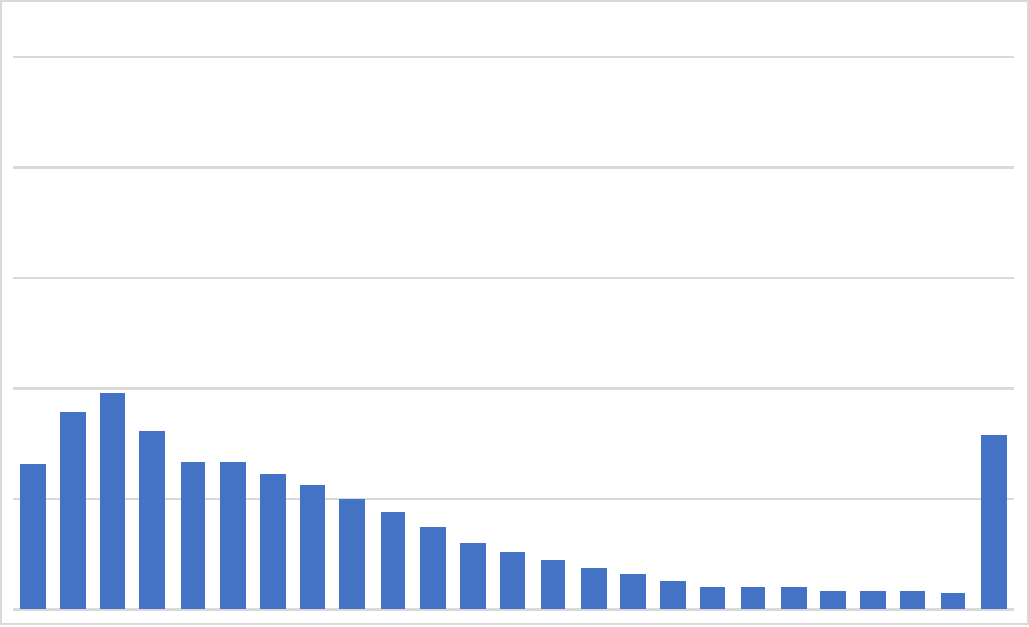
\includegraphics[width=0.9\linewidth]{results/cloverleaf3d/eul_1/Eul1_AvgL2.pdf}
\vspace{-2mm}
\caption{Eul 20 Avg$_{L2}$ L2 }
\end{subfigure}
\begin{subfigure}{0.195\textwidth}
\centering
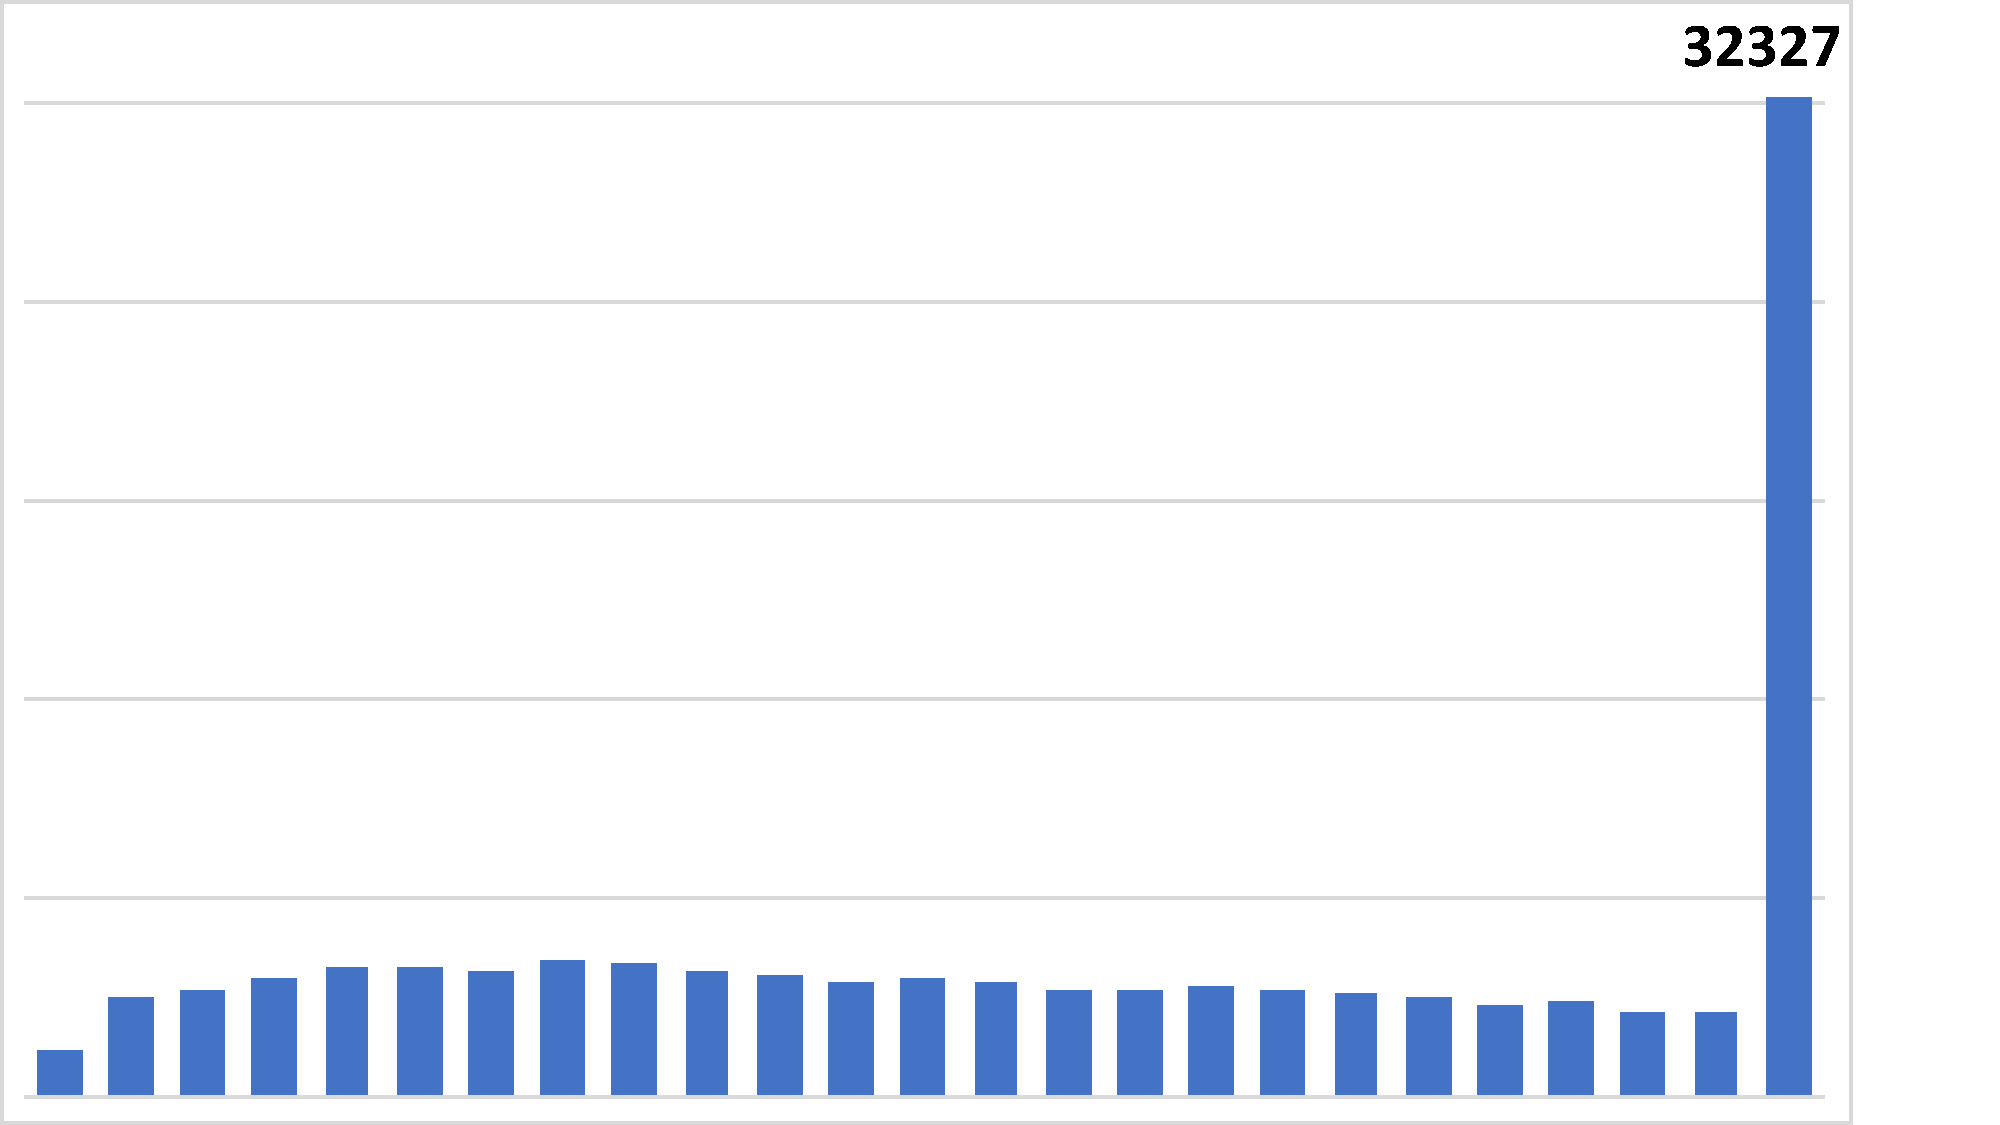
\includegraphics[width=0.95\linewidth]{results/cloverleaf3d/eul_2/Eul2_AvgL2.pdf}
\vspace{-2mm}
\caption{Eul 40 Avg$_{L2}$ L2 }
\end{subfigure}
\begin{subfigure}{0.195\textwidth}
\centering
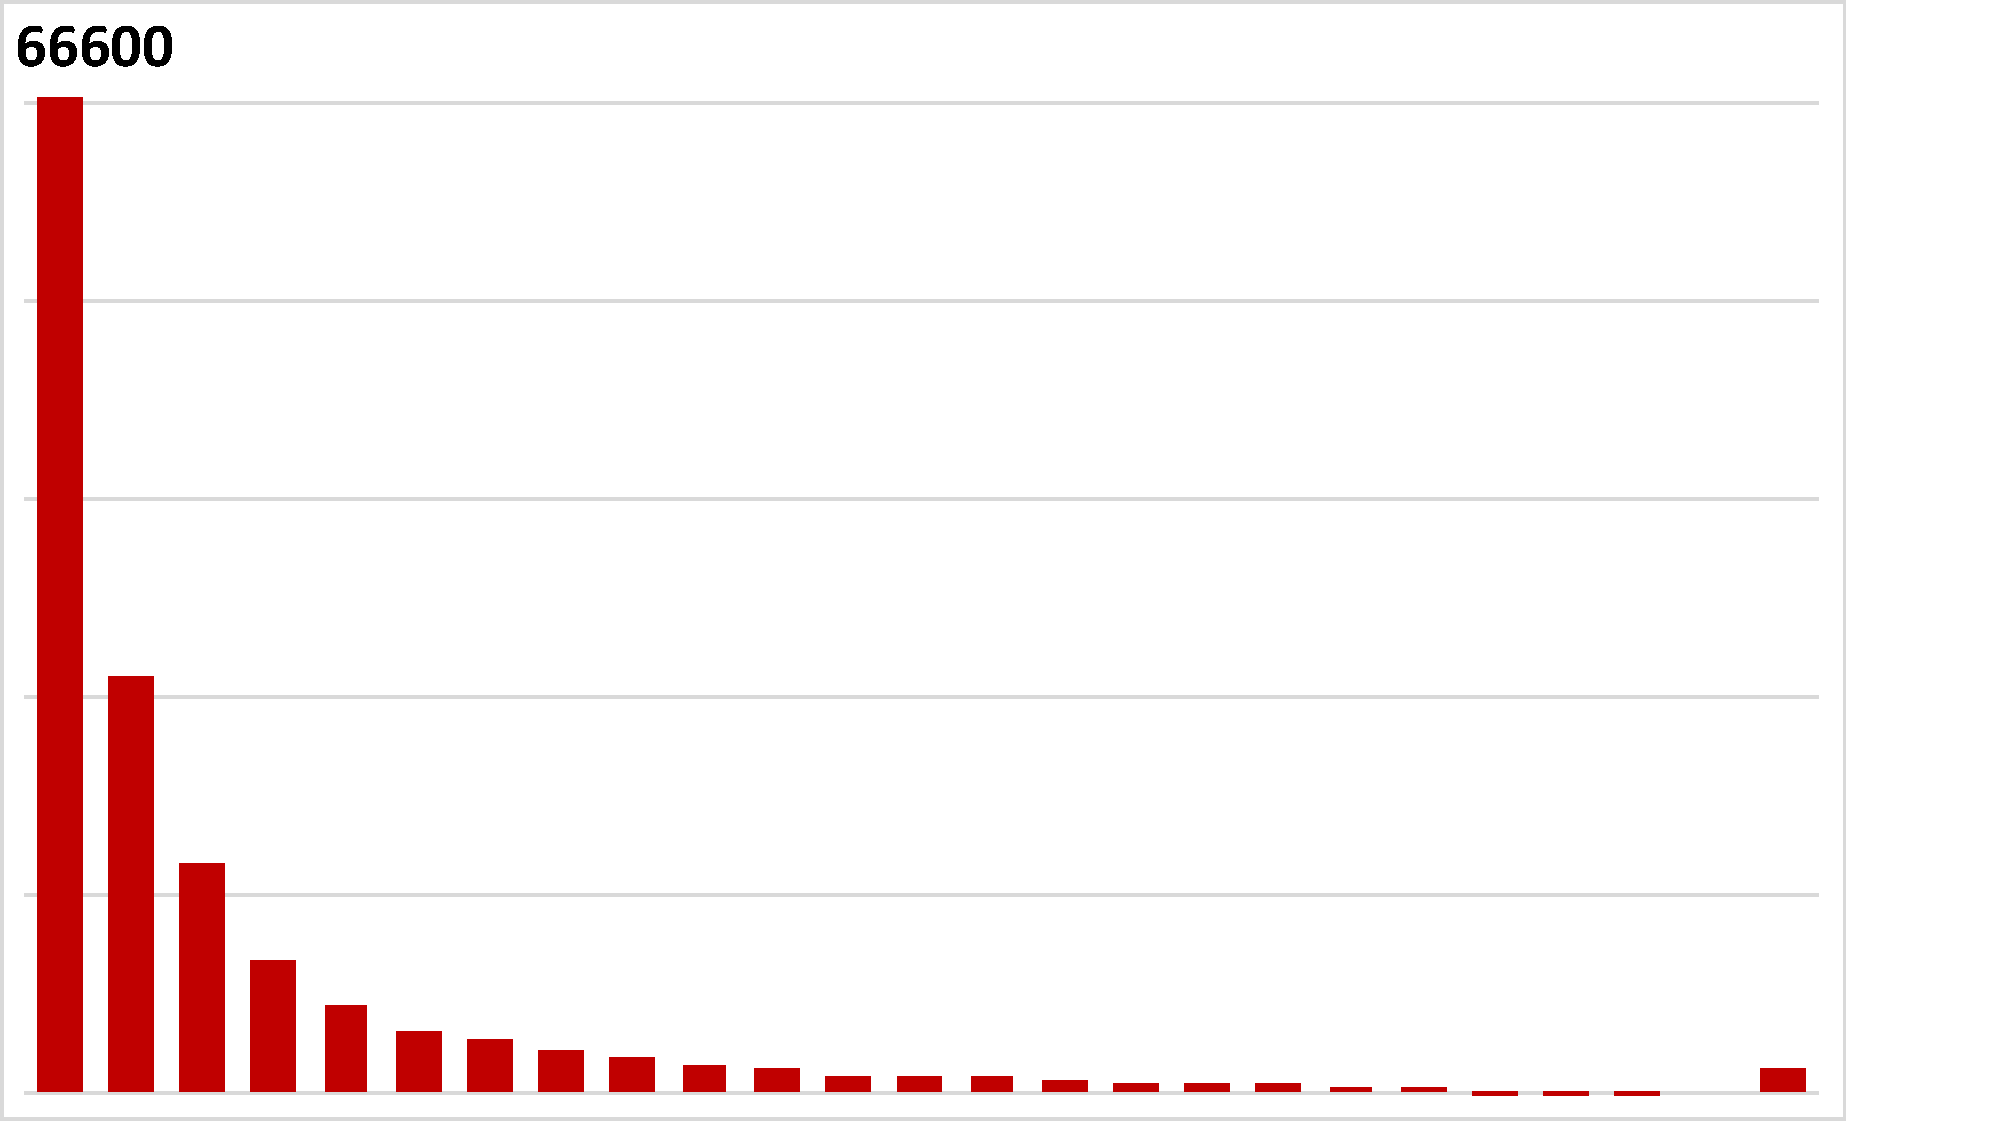
\includegraphics[width=0.9\linewidth, trim={0cm 0cm 2.5cm 0cm}, clip]{results/cloverleaf3d/lag_4/Lag4_AvgL2.pdf}
\vspace{-2mm}
\caption{Lag 40 1:8 Avg$_{L2}$ }
\end{subfigure}
\begin{subfigure}{0.195\textwidth}
\centering
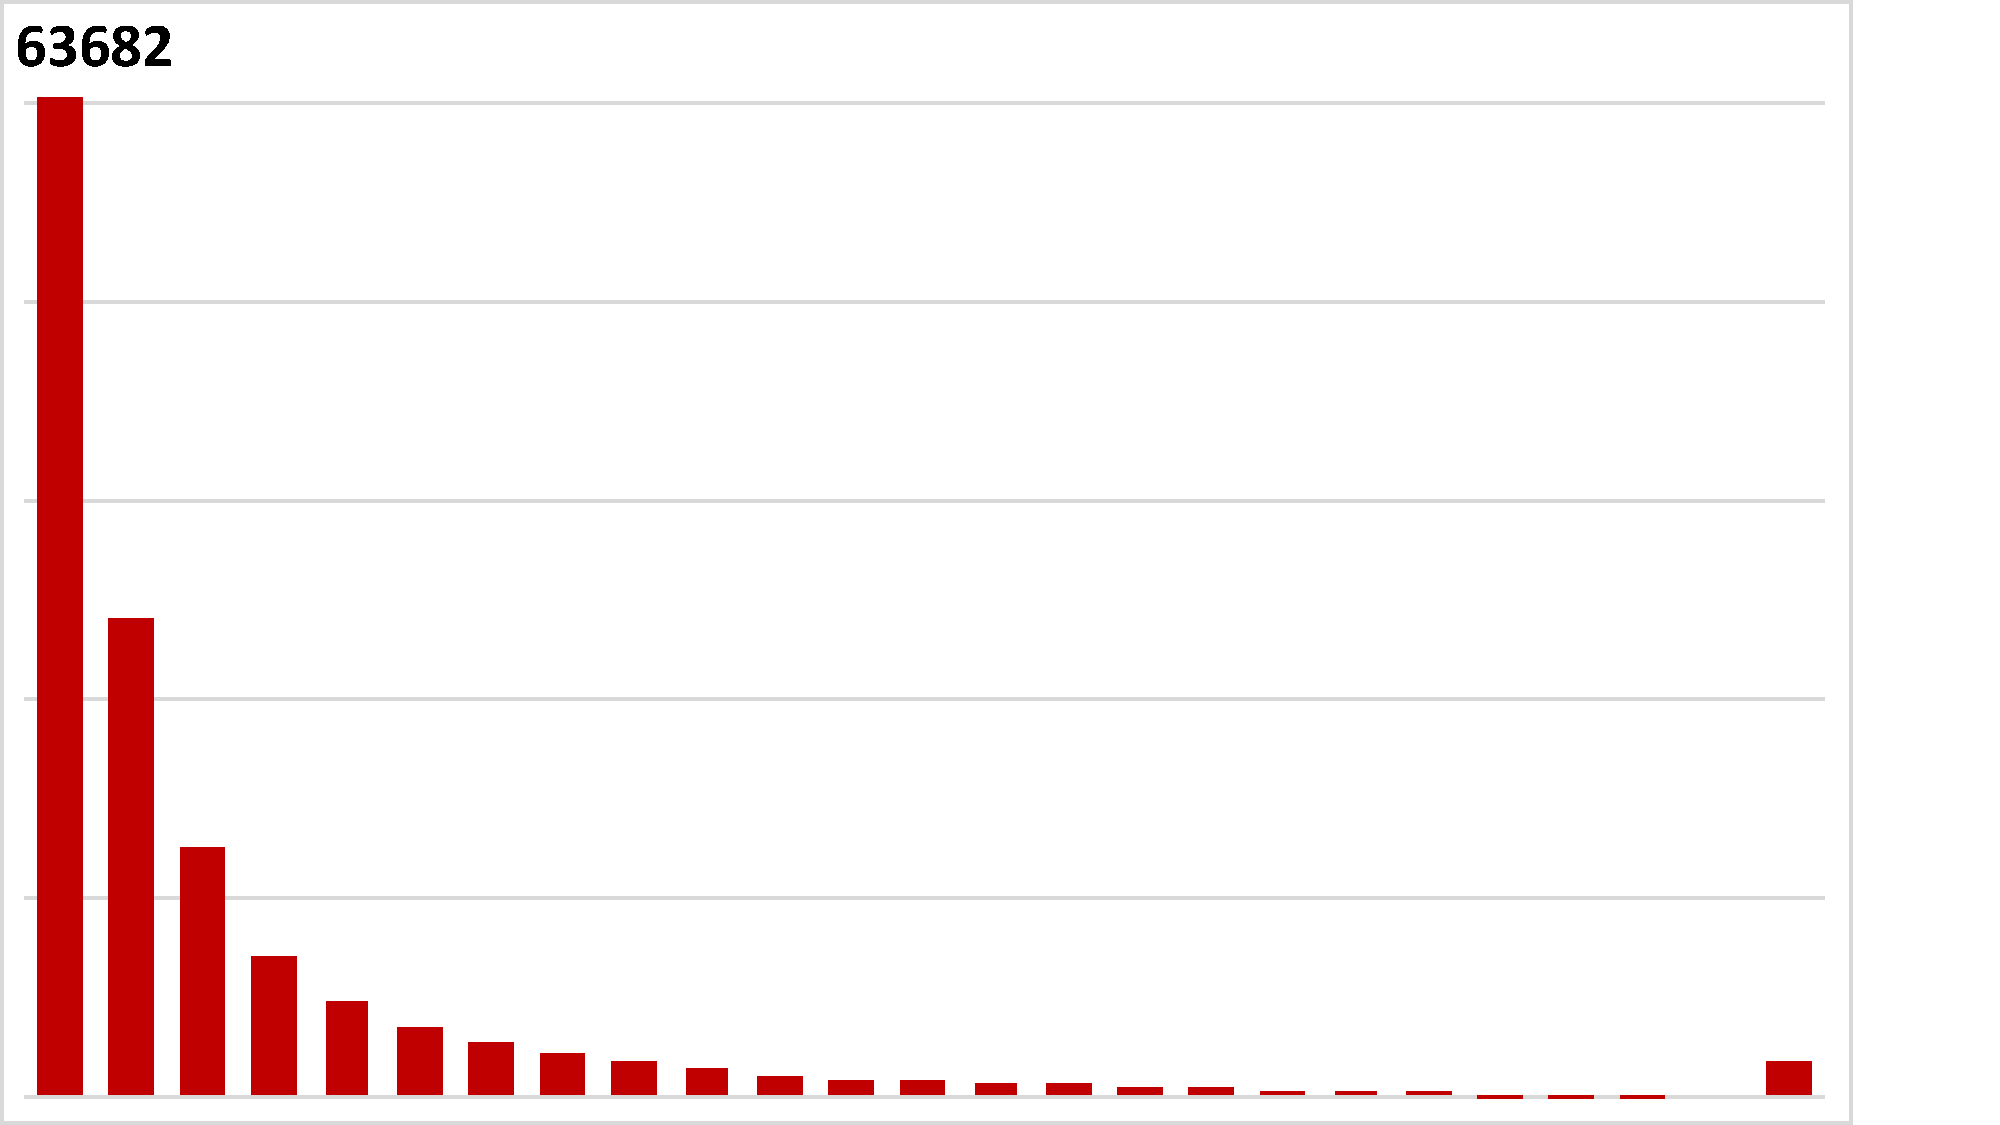
\includegraphics[width=0.9\linewidth, trim={0cm 0cm 2.5cm 0cm}, clip]{results/cloverleaf3d/lag_5/Lag5_AvgL2.pdf}
\vspace{-2mm}
\caption{Lag 40 1:27 Avg$_{L2}$ }
\end{subfigure}
\begin{subfigure}{0.195\textwidth}
\centering
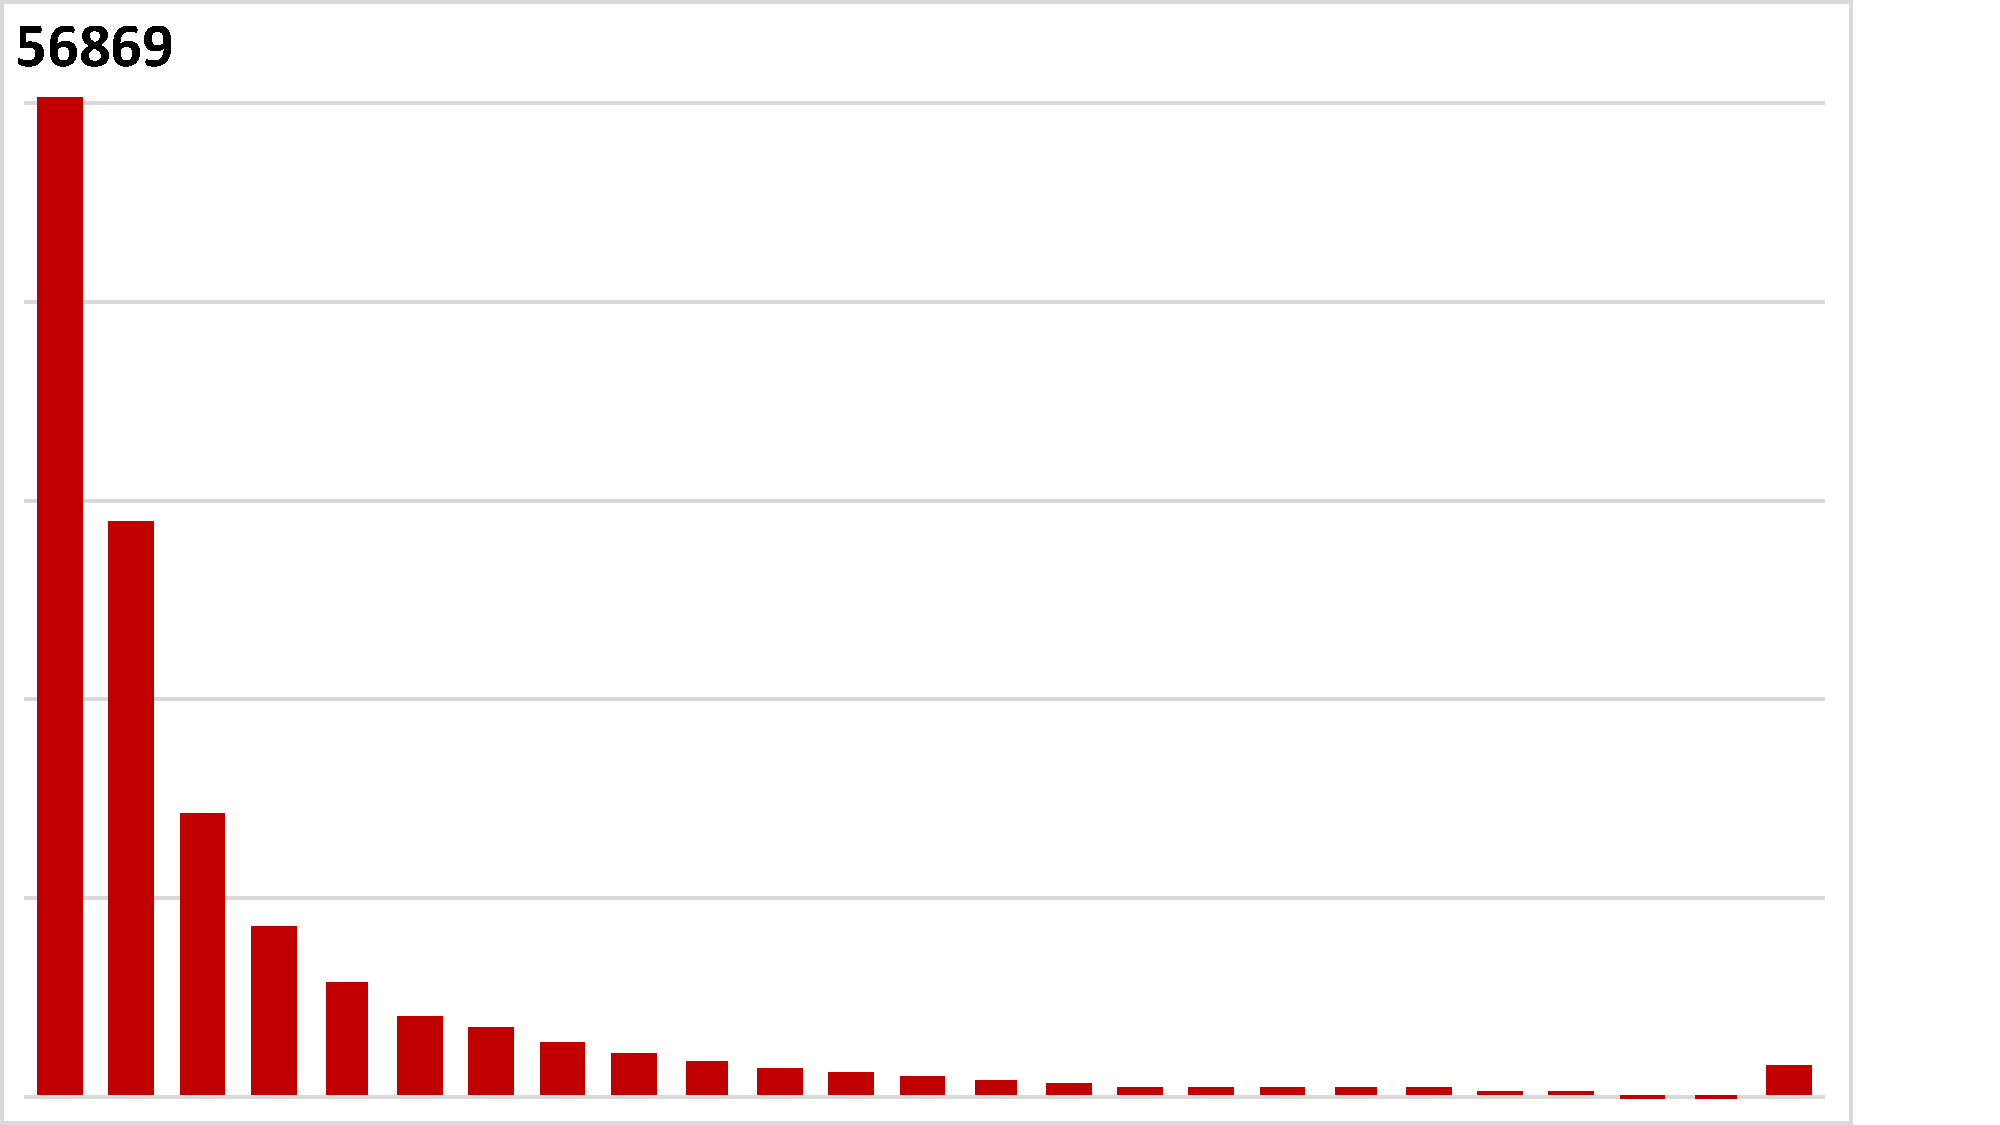
\includegraphics[width=0.9\linewidth, trim={0cm 0cm 2.5cm 0cm}, clip]{results/cloverleaf3d/lag_6/Lag6_AvgL2.pdf}
\vspace{-2mm}
\caption{Lag 40 1:64 Avg$_{L2}$ }
\end{subfigure}
\begin{subfigure}{0.195\textwidth}
\centering
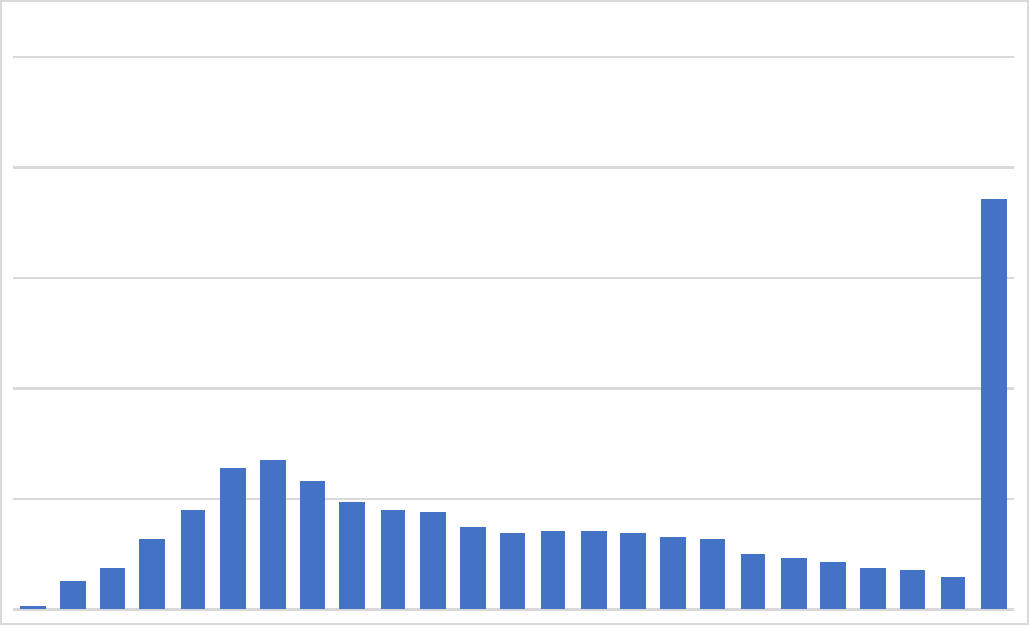
\includegraphics[width=0.9\linewidth]{results/cloverleaf3d/eul_1/Eul1_Max.pdf}
\vspace{-2mm}
\caption{Eul 20 Max$_{L2}$ }
\end{subfigure}
\begin{subfigure}{0.195\textwidth}
\centering
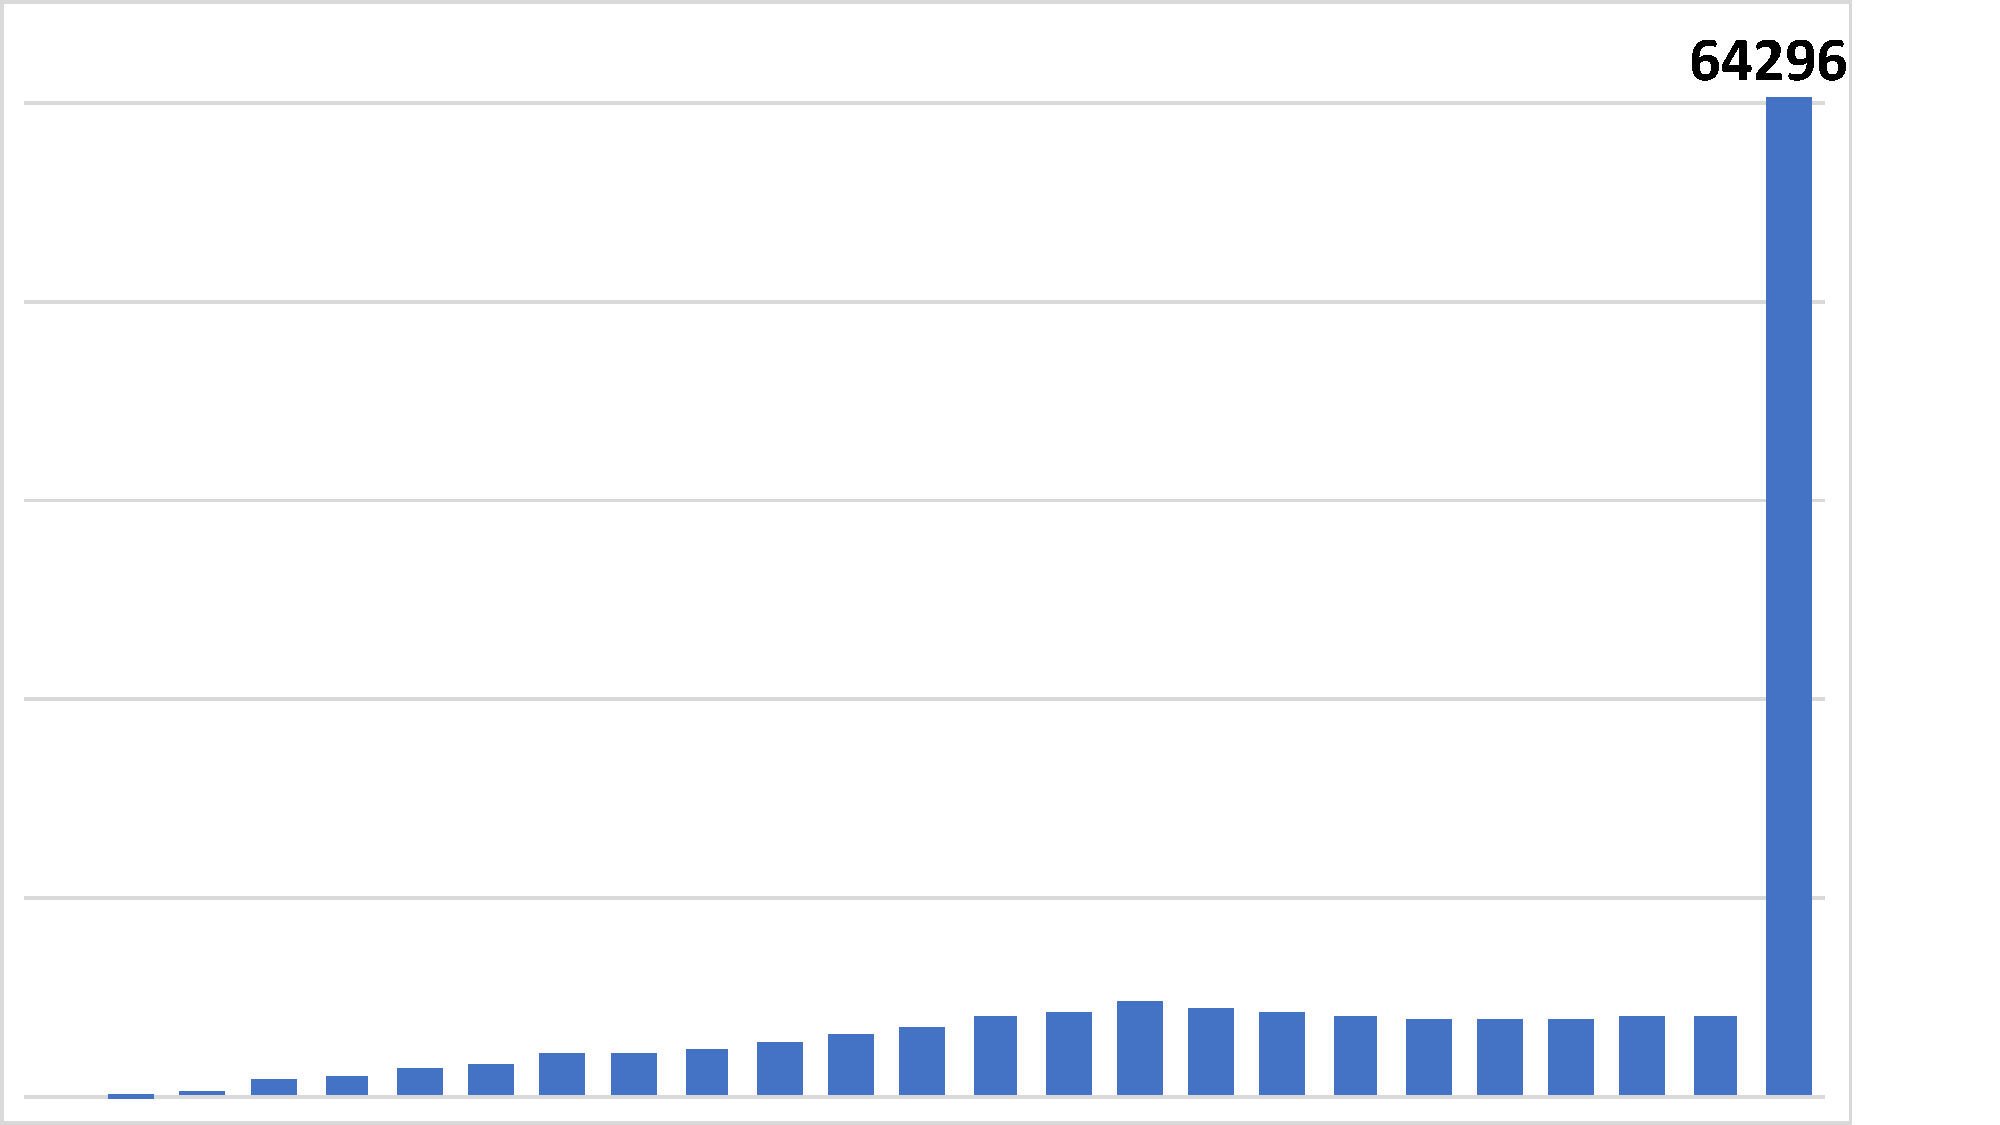
\includegraphics[width=0.95\linewidth]{results/cloverleaf3d/eul_2/Eul2_Max.pdf}
\vspace{-2mm}
\caption{Eul 40 Max$_{L2}$ }
\end{subfigure}
\hspace{0.2mm}
\begin{subfigure}{0.195\textwidth}
\centering
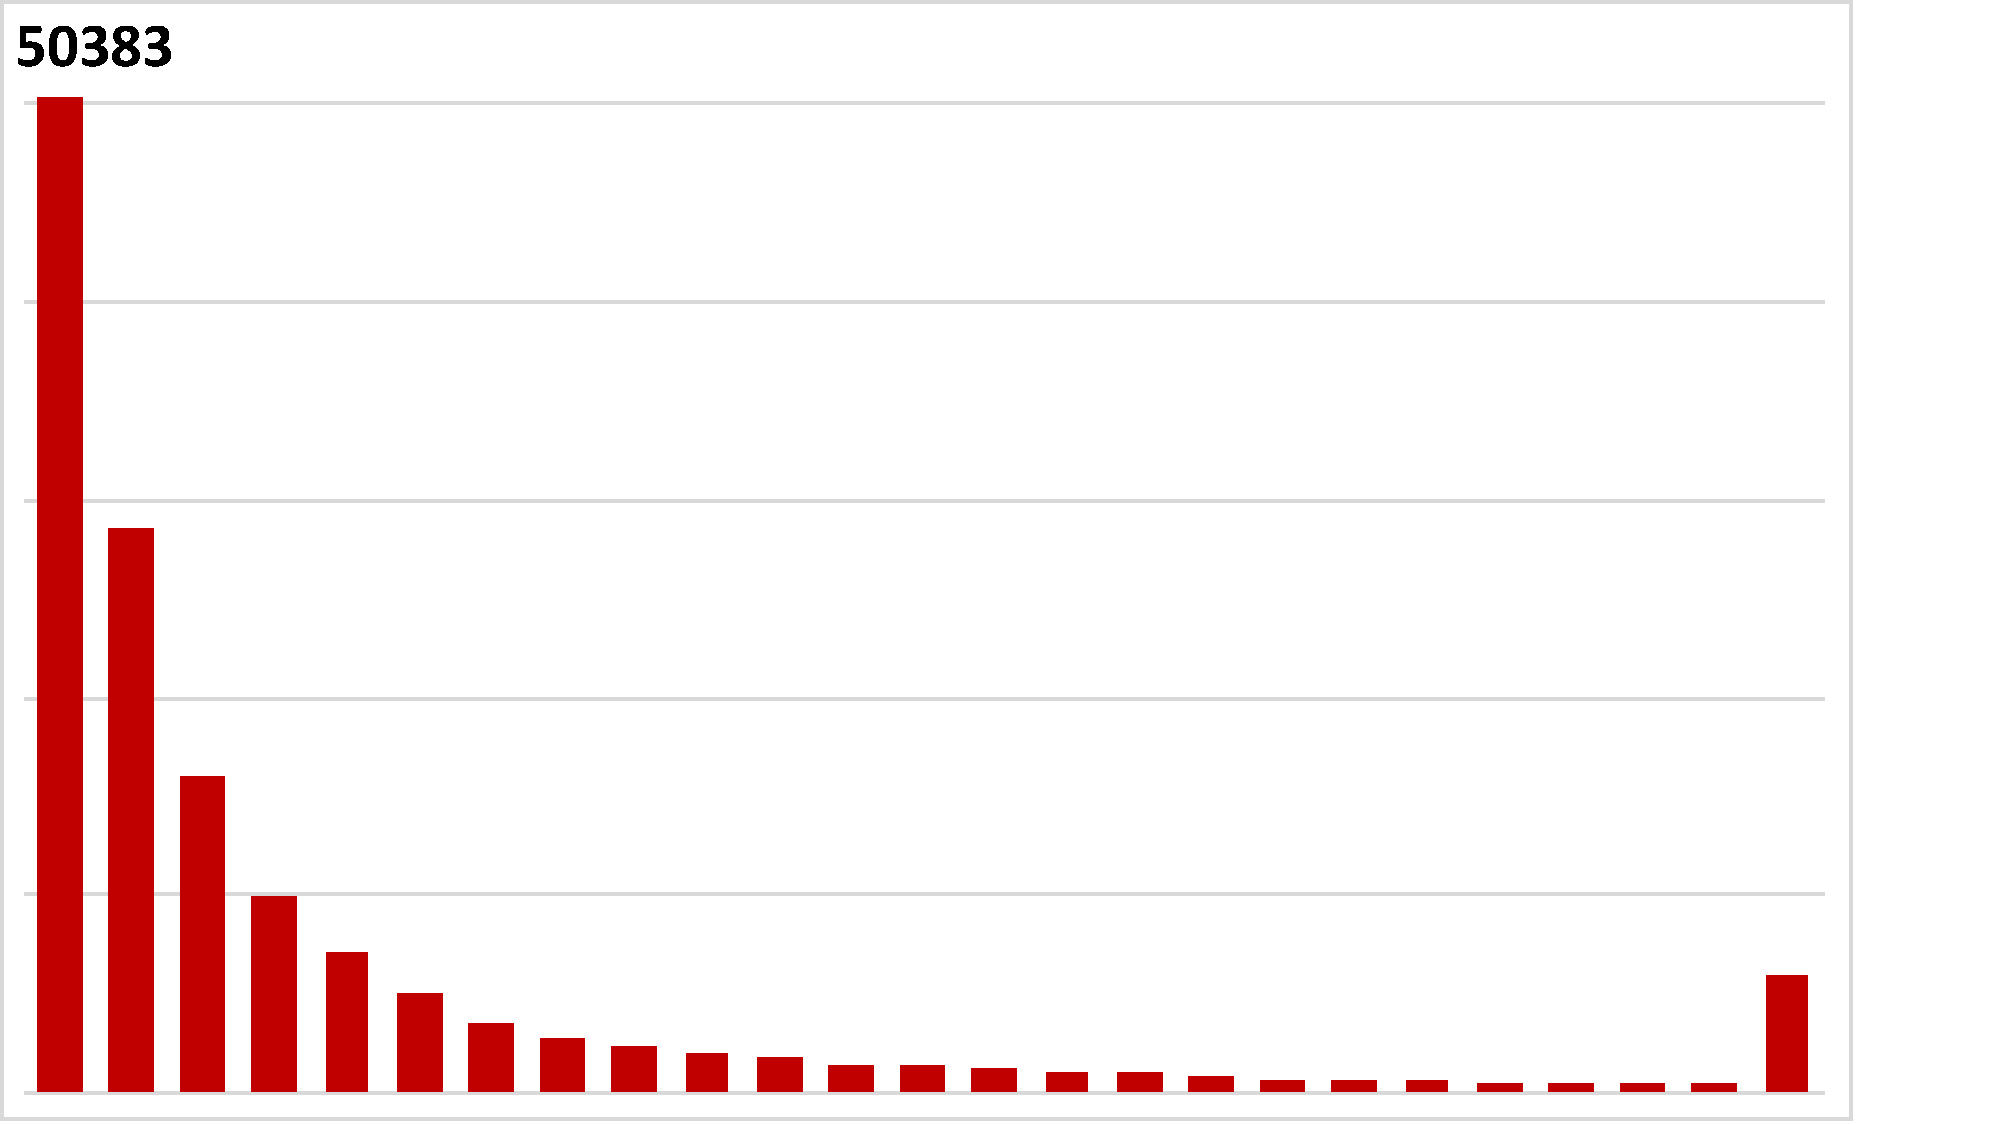
\includegraphics[width=0.9\linewidth, trim={0cm 0cm 2.5cm 0cm}, clip]{results/cloverleaf3d/lag_4/Lag4_Max.pdf}
\vspace{-2mm}
\caption{Lag 40 1:8 Max$_{L2}$ }
\end{subfigure}
\begin{subfigure}{0.195\textwidth}
\centering
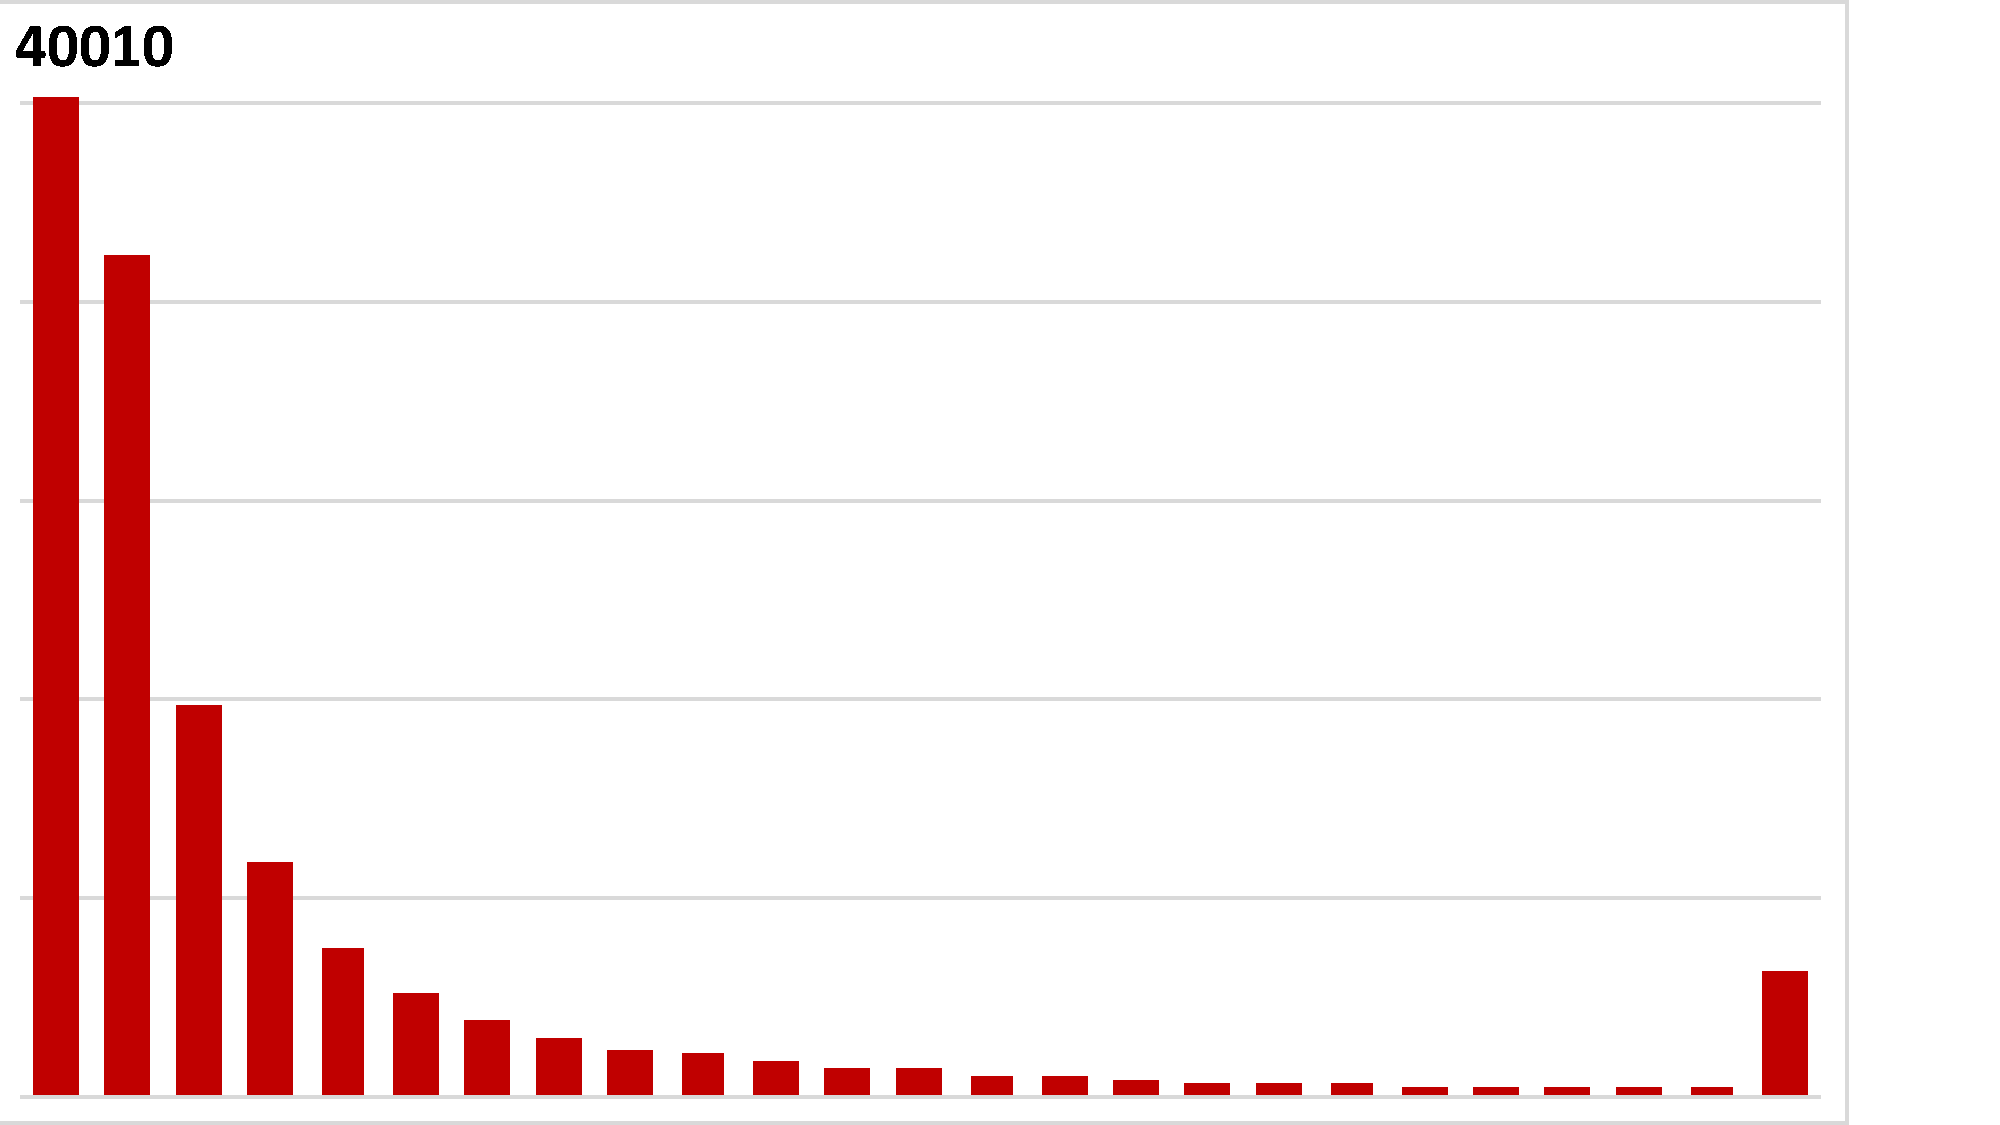
\includegraphics[width=0.9\linewidth, trim={0cm 0cm 2.5cm 0cm}, clip]{results/cloverleaf3d/lag_5/Lag5_Max.pdf}
\vspace{-2mm}
\caption{Lag 40 1:27 Max$_{L2}$}
\end{subfigure}
\begin{subfigure}{0.195\textwidth}
\centering
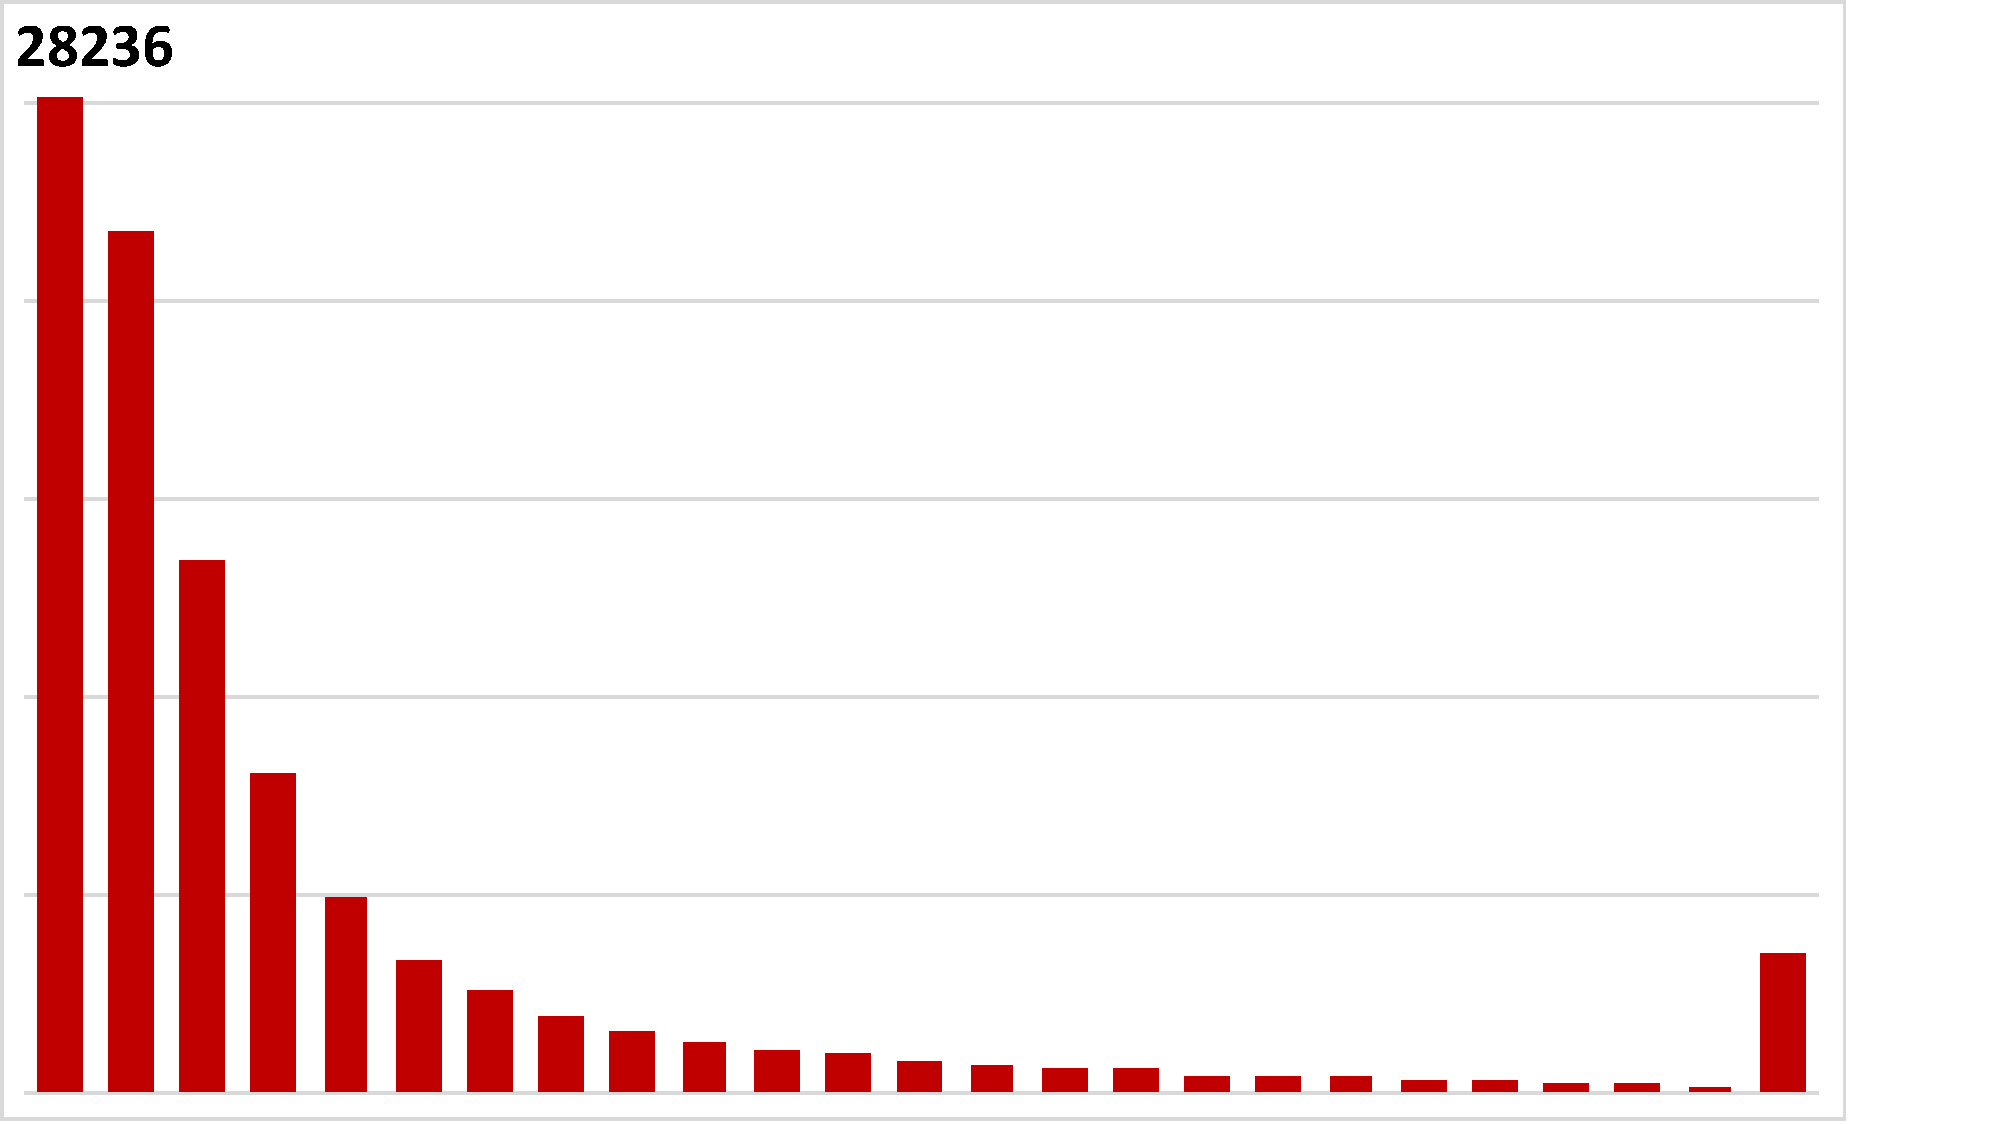
\includegraphics[width=0.9\linewidth, trim={0cm 0cm 2.5cm 0cm}, clip]{results/cloverleaf3d/lag_6/Lag6_Max.pdf}
\vspace{-2mm}
\caption{Lag 40 1:64 Max$_{L2}$}
\end{subfigure}
%\begin{subfigure}{0.24\textwidth}
%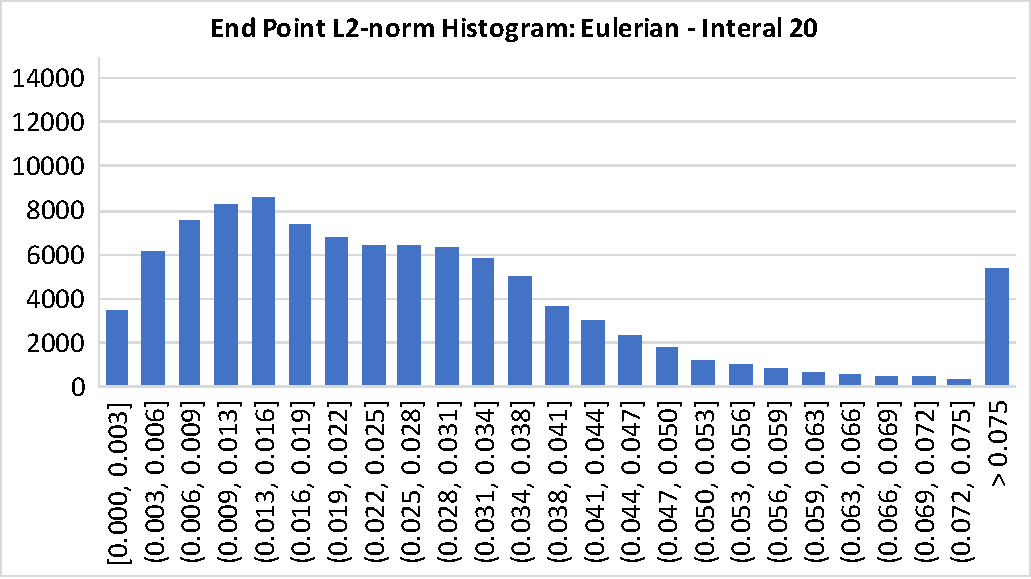
\includegraphics[width=0.9\linewidth]{results/cloverleaf3d/eul_1/Eul1_EndPt.pdf}
%\caption{Eulerian 20 End Point}
%\end{subfigure}
%\hspace{1mm}
%\begin{subfigure}{0.21\textwidth}
%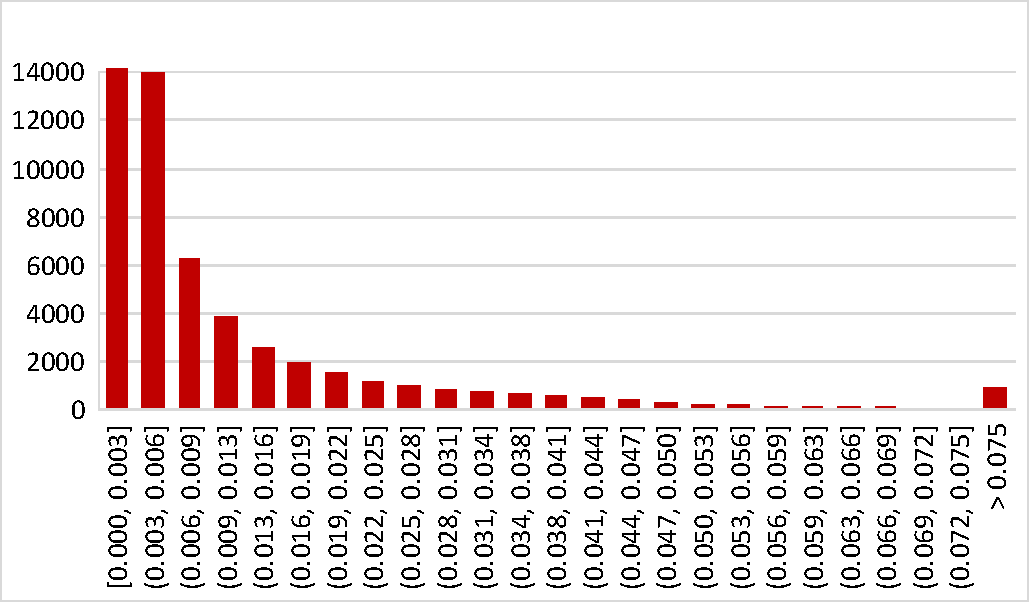
\includegraphics[width=1\linewidth]{results/cloverleaf3d/lag_4/Lag4_EndPt.pdf}
%\caption{Lagrangian 40 1:8 End Point}
%\end{subfigure}
%\hspace{1mm}
%\begin{subfigure}{0.21\textwidth}
%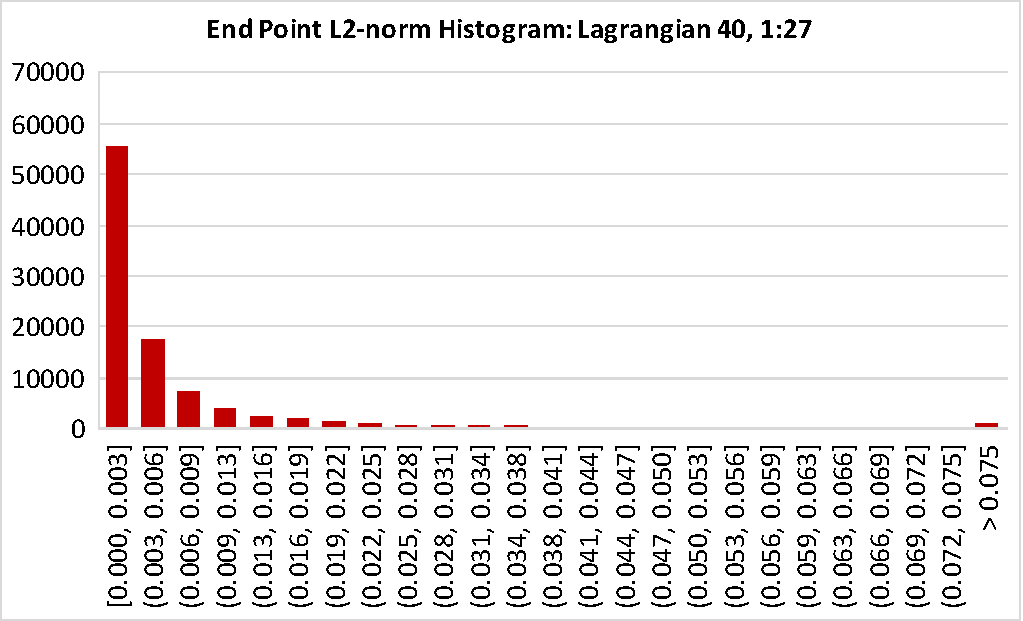
\includegraphics[width=1\linewidth]{results/cloverleaf3d/lag_5/Lag5_EndPt.pdf}
%\caption{Lagrangian 40 1:27 End Point}
%\end{subfigure}
%\hspace{1mm}
%\begin{subfigure}{0.21\textwidth}
%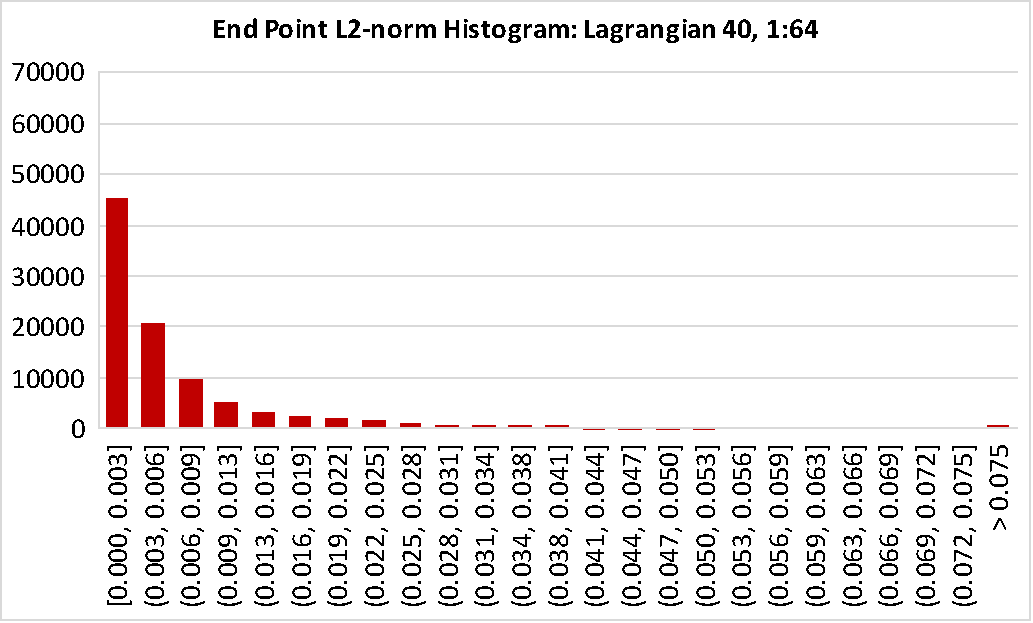
\includegraphics[width=1\linewidth]{results/cloverleaf3d/lag_6/Lag6_EndPt.pdf}
%\caption{Lagrangian 40 1:64 End Point}
%\end{subfigure}
\vspace{-3mm}
\caption{\textbf{Cloverleaf3D} experiment histograms for 100,000 test particle interpolation errors. Each plot has 25 bins, ranging from 0 to $>$0.05, with bar height encoding number of particles. Horizontal grid lines mark increments of 5,000.} 
\label{fig:clover_histograms}
\vspace{-6mm}
\end{figure*}


%\begin{figure*}
\begin{minipage}[t]{0.33\linewidth}%
\begin{framed}
\setcounter{subfigure}{0}
\begin{minipage}[t]{0.49\textwidth}%
\centering
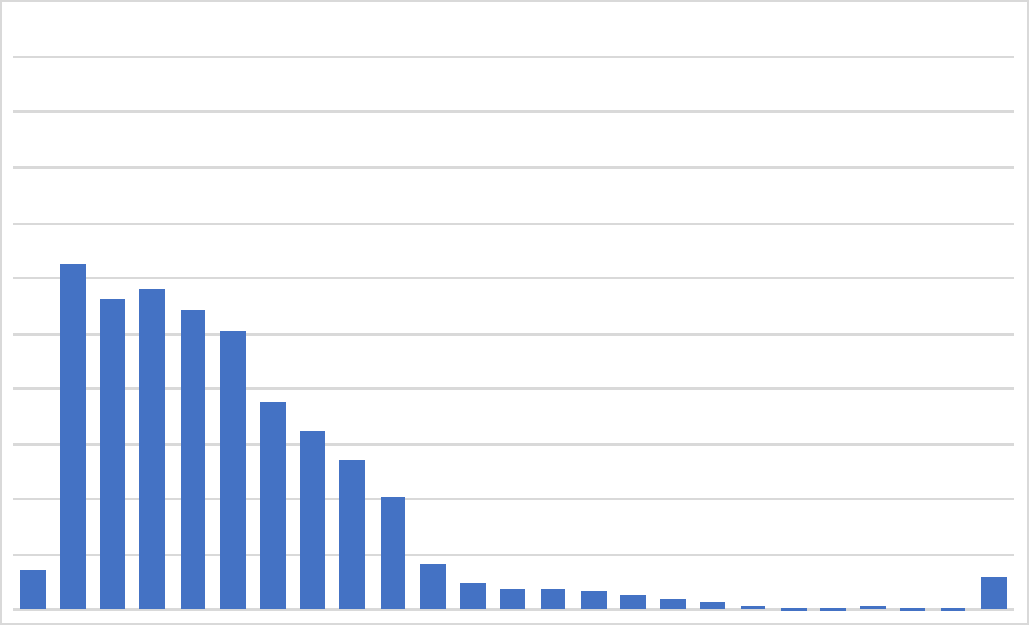
\includegraphics[width=0.95\textwidth]{results/sw4/Eul1_AvgL2.pdf}%
\vspace{-3mm}
\captionof{subfigure}{\footnotesize{Eul 250 Avg$_{L2}$}}
\end{minipage}%
\hfill
\begin{minipage}[t]{0.49\textwidth}%
\centering
\includegraphics[width=0.95\linewidth]{results/sw4/Eul2_AvgL2.pdf}
\vspace{-3mm}
\captionof{subfigure}{\footnotesize{Eul 500 Avg$_{L2}$}} 
\end{minipage}
\begin{minipage}[t]{0.49\textwidth}%
\centering
\includegraphics[width=0.95\textwidth]{results/sw4/Eul1_Max.pdf}%
\vspace{-3mm}
\captionof{subfigure}{\footnotesize{Eul 250 Max$_{L2}$}}
\end{minipage}%
\hfill
\begin{minipage}[t]{0.49\textwidth}%
\centering
\includegraphics[width=0.95\linewidth]{results/sw4/Eul2_Max.pdf}
\vspace{-3mm}
\captionof{subfigure}{\footnotesize{Eul 500 Max$_{L2}$}} 
\end{minipage}
\begin{minipage}[t]{0.49\textwidth}%
\centering
\includegraphics[width=0.95\linewidth, trim={0cm 0cm 2.5cm 0cm}, clip]{results/sw4/Lag3_AvgL2.pdf}
\vspace{-3mm}
\captionof{subfigure}{\footnotesize{Lag 250 1:27 Avg$_{L2}$}}
\end{minipage}%
\hfill
\begin{minipage}[t]{0.49\textwidth}%
\centering
\includegraphics[width=0.95\linewidth, trim={0cm 0cm 2.5cm 0cm}, clip]{results/sw4/Lag4_AvgL2.pdf}
\vspace{-3mm}
\captionof{subfigure}{\footnotesize{Lag 250 1:64 Avg$_{L2}$}} 
\end{minipage}
\begin{minipage}[t]{0.49\textwidth}%
\centering
\includegraphics[width=0.95\linewidth, trim={0cm 0cm 2.5cm 0cm}, clip]{results/sw4/Lag3_Max.pdf}
\vspace{-3mm}
\captionof{subfigure}{\footnotesize{Lag 250 1:27 Max$_{L2}$}}
\end{minipage}%
\hfill
\begin{minipage}[t]{0.49\textwidth}%
\centering
\includegraphics[width=0.95\linewidth, trim={0cm 0cm 2.5cm 0cm}, clip]{results/sw4/Lag4_Max.pdf}
\vspace{-3mm}
\captionof{subfigure}{\footnotesize{Lag 250 1:64 Max$_{L2}$}} 
\end{minipage}
\end{framed}
\vspace{-2mm}
\captionof{figure}{\textbf{SW4} experiment histograms for 90,000 test particle interpolation errors. Each plot has 25 bins, Eulerian bins range from $<$0.6 to $>$15, Lagrangian bins range from 0 to $>$0.2, with bar height encoding number of particles. Horizontal grid lines mark increments of 2,000.}
\label{fig:sw4_histograms}
\end{minipage}% End of SW4
%%%%%%%%%%%%%%%%%%%%%%%%%%%%%%%%%%%
\setcounter{subfigure}{0}
\hfill
\begin{minipage}[t]{0.66\linewidth}%
\begin{framed}
\begin{minipage}[t]{0.24\textwidth}%
\includegraphics[width=0.95\linewidth, trim={0cm 0cm 2.5cm 0cm}, clip]{results/nyx/Eul25_AvgL2.pdf}
\vspace{-2mm}
\captionof{subfigure}{Eul 25 Avg$_{L2}$}
\end{minipage}%
\hfill
\begin{minipage}[t]{0.24\textwidth}%
\includegraphics[width=0.95\linewidth, trim={0cm 0cm 2.5cm 0cm}, clip]{results/nyx/Eul50_AvgL2.pdf}
\vspace{-2mm}
\captionof{subfigure}{Eul 50 Avg$_{L2}$}
\end{minipage}
\begin{minipage}[t]{0.24\textwidth}%
\includegraphics[width=0.95\linewidth]{results/nyx/Eul100_AvgL2.pdf}
\vspace{-2mm}
\captionof{subfigure}{Eul 100 Avg$_{L2}$}
\end{minipage}%
\hfill
\begin{minipage}[t]{0.24\textwidth}%
\includegraphics[width=0.95\linewidth]{results/nyx/Eul200_AvgL2.pdf}
\vspace{-2mm}
\captionof{subfigure}{Eul 200 Avg$_{L2}$}
\end{minipage}
\begin{minipage}[t]{0.24\textwidth}%
\includegraphics[width=0.95\linewidth, trim={0cm 0cm 2.5cm 0cm}, clip]{results/nyx/Eul25_Max.pdf}
\vspace{-2mm}
\captionof{subfigure}{Eul 25 Max$_{L2}$}
\end{minipage}%
\hfill
\begin{minipage}[t]{0.24\textwidth}%
\includegraphics[width=0.95\linewidth, trim={0cm 0cm 2.5cm 0cm}, clip]{results/nyx/Eul50_Max.pdf}
\vspace{-2mm}
\captionof{subfigure}{Eul 50 Max$_{L2}$}
\end{minipage}
\begin{minipage}[t]{0.24\textwidth}%
\includegraphics[width=0.95\linewidth]{results/nyx/Eul100_Max.pdf}
\vspace{-2mm}
\captionof{subfigure}{Eul 100 Max$_{L2}$}
\end{minipage}%
\hfill
\begin{minipage}[t]{0.24\textwidth}%
\includegraphics[width=0.95\linewidth]{results/nyx/Eul200_Max.pdf}
\vspace{-2mm}
\captionof{subfigure}{Eul 200 Max$_{L2}$}
\end{minipage}
%%%% Begin Nyx Lagrangian %%% 
\begin{minipage}[t]{0.24\textwidth}%
\includegraphics[width=0.95\linewidth, trim={0cm 0cm 2.5cm 0cm}, clip]{results/nyx/Lag25_1_AvgL2.pdf}
\vspace{-2mm}
\captionof{subfigure}{Lag 25 Avg$_{L2}$}
\end{minipage}%
\hfill
\begin{minipage}[t]{0.24\textwidth}%
\includegraphics[width=0.95\linewidth, trim={0cm 0cm 2.5cm 0cm}, clip]{results/nyx/Lag50_1_AvgL2.pdf}
\vspace{-2mm}
\captionof{subfigure}{Lag 50 Avg$_{L2}$}
\end{minipage}
\begin{minipage}[t]{0.24\textwidth}%
\includegraphics[width=0.95\linewidth, trim={0cm 0cm 2.5cm 0cm}, clip]{results/nyx/Lag100_1_AvgL2.pdf}
\vspace{-2mm}
\captionof{subfigure}{Lag 100 Avg$_{L2}$}
\end{minipage}%
\hfill
\begin{minipage}[t]{0.24\textwidth}%
\includegraphics[width=0.95\linewidth, trim={0cm 0cm 2.5cm 0cm}, clip]{results/nyx/Lag200_1_AvgL2.pdf}
\vspace{-2mm}
\captionof{subfigure}{Lag 200 Avg$_{L2}$}
\end{minipage}
\begin{minipage}[t]{0.24\textwidth}%
\includegraphics[width=0.95\linewidth, trim={0cm 0cm 2.5cm 0cm}, clip]{results/nyx/Lag25_1_Max.pdf}
\vspace{-2mm}
\captionof{subfigure}{Lag 25 Max$_{L2}$}
\end{minipage}%
\hfill
\begin{minipage}[t]{0.24\textwidth}%
\includegraphics[width=0.95\linewidth, trim={0cm 0cm 2.5cm 0cm}, clip]{results/nyx/Lag50_1_Max.pdf}
\vspace{-2mm}
\captionof{subfigure}{Lag 50 Max$_{L2}$}
\end{minipage}
\begin{minipage}[t]{0.24\textwidth}%
\includegraphics[width=0.95\linewidth, trim={0cm 0cm 2.5cm 0cm}, clip]{results/nyx/Lag100_1_Max.pdf}
\vspace{-2mm}
\captionof{subfigure}{Lag 100 Max$_{L2}$}
\end{minipage}%
\hfill
\begin{minipage}[t]{0.24\textwidth}%
\includegraphics[width=0.95\linewidth, trim={0cm 0cm 2.5cm 0cm}, clip]{results/nyx/Lag200_1_Max.pdf}
\vspace{-2mm}
\captionof{subfigure}{Lag 200 Max$_{L2}$}
\end{minipage}
\end{framed}
\vspace{-2mm}
\captionof{figure}{\textbf{Nyx} experiment histograms for 50,000 test particle interpolation errors. Each plot has 20 bins, ranging from 0 to $>$0.44, with bar height encoding number of particles. Horizontal grid lines mark increments of 2,000.}
\label{fig:nyx_histograms}
\end{minipage}%
\vspace{-6mm}
\end{figure*}


\subsection{Post Hoc Efficacy}
\label{sec:results_posthoc}
\input{accuracy.tex}
\input{cloverleaf_histograms.tex}
Table~\ref{table:accuracy} contains the results of our experiments for this campaign using all three simulation codes.
%
For each simulation code we consider multiple options of number of particles and interval.
%
Varying either of these parameters impacts \textbf{PHE-1}, \textbf{PHE-2}, and \textbf{DS-1}.
%
The \textbf{Cell Side\%} column in Table~\ref{table:accuracy} redundantly encodes the value in each cell using cell background color (white to pure red hue for the range [0,100], where 0 or white indicates a particle is perfectly accurate and 100+ or pure red indicates particles on average are at least a grid cell side away from ground truth).
%
In addition to Table~\ref{table:accuracy}, our empirical study includes a more detailed look at per particle interpolation error using histograms.
%
We present a set of histograms for each simulation code. 
%
For each histogram chart we exclude the axes and instead describe the common details of the plot in the captions (number of bins, range, horizontal grid line increment, etc.) and use annotation to mark histogram bars whose height exceeds the plot area.
%
Although use of an annotation rather than the true height of the bar visually misrepresents a single data point in some plots, we believe this tradeoff is worth the closer look at the remaining data points.


%We separate our discussion of post hoc efficacy based on \textbf{PHE-1} and \textbf{PHE-2}.
%
%Our quantitative evaluation of accuracy is in Section~\ref{sec:accuracy} and post hoc distributed-memory interpolation costs are reported in Section~\ref{sec:posthoc_costs}. 
\subsubsection{Cloverleaf3D Hydrodynamics Proxy Simulation}
For the Cloverleaf3D time-dependent vector field, we considered 3 options for both number of particles and interval, to encode the behavior of the field.
%
We randomly placed 100,000 test particles in the domain and tested the accuracy of reconstructed trajectories.
%
We use the first 600 cycles of the simulation and set step size to 0.0045.
%
Overall, we observed that the Lagrangian technique performed significantly better and offered improved data storage-accuracy propositions.

With respect to \textbf{DS-1} and \textbf{PHE-1}, even a 100X data reduction results in improved accuracy compared to storing a full resolution Eulerian grid more frequently. 
%
For example, a Lagrangian configuration using 1:64 number of particles and an interval of 60 stores 1.3 GB over 600 cycles, and has an \textbf{AvgN$_{L2}$} of 41.2\% of the cell side. 
%
In comparison, an Eulerian configuration storing the full mesh every 40 cycles requires 133 GB over 600 cycles, and has an \textbf{AvgN$_{L2}$} of 270.4\% of the cell side.
%
For all the Lagrangian configurations, the \textbf{AvgN$_{L2}$} was low and particles on average remained within the same cell as the ground truth.
%

Although this proxy simulation demonstrates very clearly the shortcomings of the Eulerian technique as the interval increases, we observed that the Lagrangian technique benefits minimally from an increase in the number of particles.
%
We believe this is due to Cloverleaf3D being a miniapp, where increasing the spatial resolution does not increase the complexity of the physics, i.e., no new features are introduced as they would be in a real-world simulation.
%
That being said, even if the Eulerian technique used multi-resolution to achieve reduced storage, it would be less accurate than Lagrangian, given using the full spatial resolution is less accurate. 

The histogram plots in Figure~\ref{fig:clover_histograms} show the distribution of particle interpolation error clearly indicating the superiority of the Lagrangian technique for \textbf{EUS}.
%
Comparing the histogram plots, although Eulerian (267 GB) is storing full resolution data sets twice as often, the number of test particles with a \textbf{Max$_{L2}$} of over 300\% of the cell side distance (right-end bin in each plot) is over 15\%, compared to less than 5\% for Lagrangian (2 GB to 17 GB) in all cases.
%
This provides intuition regarding the ``rate of inaccurate interpolation'' for each technique for the \textbf{EUS} problem.

\input{reconstruction_table.tex}
For \textbf{PHE-2}, we measured the time required for Cloverleaf3D reconstructions.
%
In our empirical study, we only reconstructed Cloverleaf3D pathlines in a distributed-memory setting (16 nodes, 96 MPI ranks).
%
Table~\ref{table:reconstruction} contains timings for our reconstruction method for a single interval given a workload, i.e., number of samples to be triangulated and interpolated per rank.
%
%The total reconstruction cost \textbf{PHE-2} of entire pathlines depends on the number of intervals spanning the total number of cycles.
%
%Although shorter intervals offers higher resolution in terms of number of known interpolated points along a reconstructed pathline, longer intervals offers less total reconstruction time.
%
The most dominant cost during this process is the search structure construction, i.e., the Delaunay triangulation.
%
Although we avoid the prohibitive cost of a global Delaunay triangulation with our implementation, we believe there is room for improvement.
%
That being said, for reduced Lagrangian representations, the parallel Delaunay construction cost can be low compared to the Eulerian approach that requires performing interpolation and communication for every cycle.
%
For example, the Lagrangian configuration using an interval of 40 and 1:27 number of particles, can be used to construct pathlines for 100,000 particles across 600 cycles in under 6 minutes (excluding I/O).
%
For an Eulerian approach to be faster, it would need to compute each cycle in 0.6 seconds (our implementation required 0.47 seconds per cycle excluding I/O).



\subsubsection{SW4 Seismic Wave Propagation Simulation}
For the SW4 simulation, we considered 4 options for number of particles.
%
%The SW4 simulation is great example of a situation where the Lagrangian approach is better able to encode time-dependent vector field behavior.
%
The SW4 simulation generates a displacement vector field that captures the wave propagation modeled in the simulation. 
%
In this case, the Lagrangian representation is far better equipped than the traditional method to accurately encode this transient behavior in the domain. 
%
Our experiments considered 2000 cycles of the simulation, and evaluated accuracy by reconstructing 90,000 test particle trajectories placed randomly between Z=5,000 and Z=15,000 (the layer of most activity in the domain) using a step size of 1.

The SW4 simulation domain extents are very large, thus each cell side is approximately 387 in our experiments.
%
The \textbf{AvgN$_{L2}$} value of our test particles indicates all particles remained within the cell, with the Lagrangian technique offering near perfect reconstruction, while the Eulerian technique only suffers from an error of 1\% of the cell side by this measure.
%
However, displacement values in an earthquake simulation are expected to be small and an error of even that magnitude might represent failure to capture the wave propagation.
%

The SW4 histogram plots (Figure~\ref{fig:sw4_histograms}) use different bin ranges for Lagrangian and Eulerian given the distributions were very different.
%
The plots show the an increase in error for the Eulerian technique as the interval increases and an increase in error for the Lagrangian technique as the number of particles used decreases from 1:27 to 1:64.
%

Overall, the Lagrangian technique offers excellent propositions for \textbf{DS-1} and \textbf{PHE-1}.
%
The Lagrangian technique was able to preserve near perfect integrity with upto 70X less data storage.
\subsubsection{Nyx Cosmology Simulation}
For the Nyx cosmology simulation, we considered 4 options for number of particles and interval to provide an understanding across a wider spatiotemporal range.
%
Figure~\ref{fig:vectorfield_nyx} shows a slice of the Nyx vector field at two three slices~(0, 200, 400).
%
We observed that the unit vectors at each grid point in the domain remain relatively the same across all cycles.
%
The slow evolution of the vector field is in terms of velocity magnitude in few regions of the domain.
%
The maximum velocity magnitude in the domain increases steadily for the 400 cycles of the simulation we use in this study.
%
Our experiments considered 50,000 test particle trajectories placed randomly in the domain and set a step size to 0.02.
\input{vectorfield_nyx.tex}

\input{histogram_plots.tex}

An interesting outcome of these experiments was observing \textbf{PHE-1}, i.e., accuracy, given the variation in interval.
%
The Eulerian technique is nearly perfectly accurate when the sampling is less sparse (interval = 25).
%
In contrast, the Lagrangian technique is less accurate, even when using the same number of particles as grid points.
%
Such behavior is expected when the variation between the vector field across cycles is very small (Figure~\ref{fig:vectorfield_nyx}).
%
In such a setting, using only a fourth-order Runge Kutta (RK4) provides more accurate interpolation than applying a second-order barycentric coordinates interpolation on top of the trajectories extracted using RK4.
%
This ``stitching'' error has been studied in several prior works~\cite{hlawatsch2011hierarchical,bujack2015lagrangian,hummel2016error, sane2019interpolation}.
\input{nyx_vis.tex}

As the interval size increases, i.e., the \textbf{S}parsity component of the \textbf{EUS} problem, we observe Lagrangian improving in accuracy and offering multiple favorable data storage-accuracy propositions.
%
For example, for an interval of 200, greater accuracy can be achieved by the Lagrangian technique using a 10X data reduction.
%
The behavior of techniques (one losing integrity as sparsity increases; another becoming more accurate as sparsity increases) is well captured by the histograms in Figure~\ref{fig:nyx_histograms}.
%
Of course, a longer interval does not guarantee better accuracy for the Lagrangian technique in all settings.
%
Divergence over a long interval impacts Lagrangian-based interpolation accuracy~\cite{chandler2016analysis}.

With respect to the impact of number of particles on \textbf{PHE-1} and \textbf{DS-1}, we observe that error increases due to data reductions are higher when the interval is smaller. 
%
For example, error increases by 3X for a 27X data reduction for interval 200 and error increases by over 6X for a 27X data reduction for interval 25.
%
We note that in each of these cases, the increases in error resulted in \textbf{AvgN$_{L2}$} values that still indicate that the majority of test particles were within the same cell as the ground truth particle.
%
This result supports the notion that the Lagrangian technique can effectively support data reduction in settings of temporal sparsity.
%
Overall, our empirical study using the derived Nyx vector field produced interesting trends that support the use of Lagrangian technique for \textbf{EUS} problem, while also demonstrating a stitching error when storing data to disk more frequently.


%\begin{figure*}
\begin{minipage}[t]{0.33\linewidth}%
\begin{framed}
\setcounter{subfigure}{0}
\begin{minipage}[t]{0.49\textwidth}%
\centering
\includegraphics[width=0.95\textwidth]{results/sw4/Eul1_AvgL2.pdf}%
\vspace{-3mm}
\captionof{subfigure}{\footnotesize{Eul 250 Avg$_{L2}$}}
\end{minipage}%
\hfill
\begin{minipage}[t]{0.49\textwidth}%
\centering
\includegraphics[width=0.95\linewidth]{results/sw4/Eul2_AvgL2.pdf}
\vspace{-3mm}
\captionof{subfigure}{\footnotesize{Eul 500 Avg$_{L2}$}} 
\end{minipage}
\begin{minipage}[t]{0.49\textwidth}%
\centering
\includegraphics[width=0.95\textwidth]{results/sw4/Eul1_Max.pdf}%
\vspace{-3mm}
\captionof{subfigure}{\footnotesize{Eul 250 Max$_{L2}$}}
\end{minipage}%
\hfill
\begin{minipage}[t]{0.49\textwidth}%
\centering
\includegraphics[width=0.95\linewidth]{results/sw4/Eul2_Max.pdf}
\vspace{-3mm}
\captionof{subfigure}{\footnotesize{Eul 500 Max$_{L2}$}} 
\end{minipage}
\begin{minipage}[t]{0.49\textwidth}%
\centering
\includegraphics[width=0.95\linewidth, trim={0cm 0cm 2.5cm 0cm}, clip]{results/sw4/Lag3_AvgL2.pdf}
\vspace{-3mm}
\captionof{subfigure}{\footnotesize{Lag 250 1:27 Avg$_{L2}$}}
\end{minipage}%
\hfill
\begin{minipage}[t]{0.49\textwidth}%
\centering
\includegraphics[width=0.95\linewidth, trim={0cm 0cm 2.5cm 0cm}, clip]{results/sw4/Lag4_AvgL2.pdf}
\vspace{-3mm}
\captionof{subfigure}{\footnotesize{Lag 250 1:64 Avg$_{L2}$}} 
\end{minipage}
\begin{minipage}[t]{0.49\textwidth}%
\centering
\includegraphics[width=0.95\linewidth, trim={0cm 0cm 2.5cm 0cm}, clip]{results/sw4/Lag3_Max.pdf}
\vspace{-3mm}
\captionof{subfigure}{\footnotesize{Lag 250 1:27 Max$_{L2}$}}
\end{minipage}%
\hfill
\begin{minipage}[t]{0.49\textwidth}%
\centering
\includegraphics[width=0.95\linewidth, trim={0cm 0cm 2.5cm 0cm}, clip]{results/sw4/Lag4_Max.pdf}
\vspace{-3mm}
\captionof{subfigure}{\footnotesize{Lag 250 1:64 Max$_{L2}$}} 
\end{minipage}
\end{framed}
\vspace{-2mm}
\captionof{figure}{\textbf{SW4} experiment histograms for 90,000 test particle interpolation errors. Each plot has 25 bins, Eulerian bins range from $<$0.6 to $>$15, Lagrangian bins range from 0 to $>$0.2, with bar height encoding number of particles. Horizontal grid lines mark increments of 2,000.}
\label{fig:sw4_histograms}
\end{minipage}% End of SW4
%%%%%%%%%%%%%%%%%%%%%%%%%%%%%%%%%%%
\setcounter{subfigure}{0}
\hfill
\begin{minipage}[t]{0.66\linewidth}%
\begin{framed}
\begin{minipage}[t]{0.24\textwidth}%
\includegraphics[width=0.95\linewidth, trim={0cm 0cm 2.5cm 0cm}, clip]{results/nyx/Eul25_AvgL2.pdf}
\vspace{-2mm}
\captionof{subfigure}{Eul 25 Avg$_{L2}$}
\end{minipage}%
\hfill
\begin{minipage}[t]{0.24\textwidth}%
\includegraphics[width=0.95\linewidth, trim={0cm 0cm 2.5cm 0cm}, clip]{results/nyx/Eul50_AvgL2.pdf}
\vspace{-2mm}
\captionof{subfigure}{Eul 50 Avg$_{L2}$}
\end{minipage}
\begin{minipage}[t]{0.24\textwidth}%
\includegraphics[width=0.95\linewidth]{results/nyx/Eul100_AvgL2.pdf}
\vspace{-2mm}
\captionof{subfigure}{Eul 100 Avg$_{L2}$}
\end{minipage}%
\hfill
\begin{minipage}[t]{0.24\textwidth}%
\includegraphics[width=0.95\linewidth]{results/nyx/Eul200_AvgL2.pdf}
\vspace{-2mm}
\captionof{subfigure}{Eul 200 Avg$_{L2}$}
\end{minipage}
\begin{minipage}[t]{0.24\textwidth}%
\includegraphics[width=0.95\linewidth, trim={0cm 0cm 2.5cm 0cm}, clip]{results/nyx/Eul25_Max.pdf}
\vspace{-2mm}
\captionof{subfigure}{Eul 25 Max$_{L2}$}
\end{minipage}%
\hfill
\begin{minipage}[t]{0.24\textwidth}%
\includegraphics[width=0.95\linewidth, trim={0cm 0cm 2.5cm 0cm}, clip]{results/nyx/Eul50_Max.pdf}
\vspace{-2mm}
\captionof{subfigure}{Eul 50 Max$_{L2}$}
\end{minipage}
\begin{minipage}[t]{0.24\textwidth}%
\includegraphics[width=0.95\linewidth]{results/nyx/Eul100_Max.pdf}
\vspace{-2mm}
\captionof{subfigure}{Eul 100 Max$_{L2}$}
\end{minipage}%
\hfill
\begin{minipage}[t]{0.24\textwidth}%
\includegraphics[width=0.95\linewidth]{results/nyx/Eul200_Max.pdf}
\vspace{-2mm}
\captionof{subfigure}{Eul 200 Max$_{L2}$}
\end{minipage}
%%%% Begin Nyx Lagrangian %%% 
\begin{minipage}[t]{0.24\textwidth}%
\includegraphics[width=0.95\linewidth, trim={0cm 0cm 2.5cm 0cm}, clip]{results/nyx/Lag25_1_AvgL2.pdf}
\vspace{-2mm}
\captionof{subfigure}{Lag 25 Avg$_{L2}$}
\end{minipage}%
\hfill
\begin{minipage}[t]{0.24\textwidth}%
\includegraphics[width=0.95\linewidth, trim={0cm 0cm 2.5cm 0cm}, clip]{results/nyx/Lag50_1_AvgL2.pdf}
\vspace{-2mm}
\captionof{subfigure}{Lag 50 Avg$_{L2}$}
\end{minipage}
\begin{minipage}[t]{0.24\textwidth}%
\includegraphics[width=0.95\linewidth, trim={0cm 0cm 2.5cm 0cm}, clip]{results/nyx/Lag100_1_AvgL2.pdf}
\vspace{-2mm}
\captionof{subfigure}{Lag 100 Avg$_{L2}$}
\end{minipage}%
\hfill
\begin{minipage}[t]{0.24\textwidth}%
\includegraphics[width=0.95\linewidth, trim={0cm 0cm 2.5cm 0cm}, clip]{results/nyx/Lag200_1_AvgL2.pdf}
\vspace{-2mm}
\captionof{subfigure}{Lag 200 Avg$_{L2}$}
\end{minipage}
\begin{minipage}[t]{0.24\textwidth}%
\includegraphics[width=0.95\linewidth, trim={0cm 0cm 2.5cm 0cm}, clip]{results/nyx/Lag25_1_Max.pdf}
\vspace{-2mm}
\captionof{subfigure}{Lag 25 Max$_{L2}$}
\end{minipage}%
\hfill
\begin{minipage}[t]{0.24\textwidth}%
\includegraphics[width=0.95\linewidth, trim={0cm 0cm 2.5cm 0cm}, clip]{results/nyx/Lag50_1_Max.pdf}
\vspace{-2mm}
\captionof{subfigure}{Lag 50 Max$_{L2}$}
\end{minipage}
\begin{minipage}[t]{0.24\textwidth}%
\includegraphics[width=0.95\linewidth, trim={0cm 0cm 2.5cm 0cm}, clip]{results/nyx/Lag100_1_Max.pdf}
\vspace{-2mm}
\captionof{subfigure}{Lag 100 Max$_{L2}$}
\end{minipage}%
\hfill
\begin{minipage}[t]{0.24\textwidth}%
\includegraphics[width=0.95\linewidth, trim={0cm 0cm 2.5cm 0cm}, clip]{results/nyx/Lag200_1_Max.pdf}
\vspace{-2mm}
\captionof{subfigure}{Lag 200 Max$_{L2}$}
\end{minipage}
\end{framed}
\vspace{-2mm}
\captionof{figure}{\textbf{Nyx} experiment histograms for 50,000 test particle interpolation errors. Each plot has 20 bins, ranging from 0 to $>$0.44, with bar height encoding number of particles. Horizontal grid lines mark increments of 2,000.}
\label{fig:nyx_histograms}
\end{minipage}%
\vspace{-6mm}
\end{figure*}

%\begingroup
\setlength{\tabcolsep}{0pt}
%\renewcommand{\arraystretch}{0.55} % Default value: 1
%\setlength{\fboxsep}{1mm}
\begin{table*}[t]
\centering
\begin{tabular}{|P{2cm}|P{1.3cm}|P{2cm}|L{1.3cm} P{1.7cm} D |P{8cm}|}
\hline
Technique & Interval & Reduction & Data & AvgN$_{L2}$ & Cell  & \multirow{2}{*}{Scatter Plot} \\
& & & & & Side\% & \\
\hline
\multicolumn{6}{l}{\textbf{          Cloverleaf3D Proxy Hydrodynamics Application }} & \multirow{12}{*}{\includegraphics[width=0.95\linewidth]{images/cloverleaf_accuracy.pdf}}\\
\cline{1-6}
\multirow{3}{*}{Eulerian} & 20 & \multirow{3}{*}{Full Res} & 267 GB & 0.0197 & 116.17 &  \\
\cline{2-2}
& 40 & & 133 GB & 0.0459 & 270.49 & \\
\cline{2-2}
& 60 & & 95 GB & 0.0725 & 426.96 &  \\
\cline{1-6}
\multirow{9}{*}{Lagrangian} & \multirow{3}{*}{20} & 1:8 & 34 GB & 0.0032 & 18.928 & \\
\cline{3-3}
 & & 1:27 & 10 GB & 0.0040 & 23.891 & \\
\cline{3-3}
 & & 1:64 & 4 GB & 0.0040 & 23.583 & \\
\cline{2-3}
& \multirow{3}{*}{40} & 1:8 & 17 GB & 0.0043 & 25.646 &  \\
\cline{3-3}
& & 1:27 & 5.1 GB & 0.0049 & 29.145 &  \\
\cline{3-3}
& & 1:64 & 2 GB & 0.0053 & 31.353 & \\
\cline{2-3}
& \multirow{3}{*}{60} & 1:8 & 12 GB & 0.0064 & 37.882 & \\
\cline{3-3}
& & 1:27 & 3.4 GB & 0.0066 & 39.002 & \multirow{6}{*}{\raisebox{-33.5mm}[0pt][0pt]{\includegraphics[width=0.95\linewidth]{images/sw4_accuracy.pdf}}} \\
\cline{3-3}
& & 1:64 & 1.3 GB & 0.0070 & 41.247 & \\
\cline{1-6}
\multicolumn{6}{l}{\textbf{          SW4 Seismic Wave Modeling Simulation }} &  \\
\cline{1-6}
\multirow{2}{*}{Eulerian} & 250 & \multirow{2}{*}{Full Res} & 1100 MB & 3.5714 & 0.9224 & \\
\cline{2-2}
 & 500 & & 550 MB & 5.0493 & 1.3023  & \\
\cline{1-6}
\multirow{4}{*}{Lagrangian} & \multirow{4}{*}{250} & 1:1 & 1300 MB & 0.0005 & 0.0001  &  \\
\cline{3-3}
 &  & 1:8 & 158 MB & 0.0033 & 0.0008 &  \\
\cline{3-3}
 &  & 1:27 & 42 MB & 0.0072 & 0.0018 & \\
\cline{3-3}
 &  & 1:64 & 16 MB & 0.0128 & 0.0031 &  \\
\cline{1-6}
\multicolumn{6}{l}{\textbf{          Nyx Cosmology Simulation }} & \\
\cline{1-6}
\multirow{4}{*}{Eulerian} & 25 & \multirow{4}{*}{Full Res} & 227 MB & 0.010 & 2.2954 &  \\
\cline{2-2}%\cline{4-6}
& 50 & & 120 MB & 0.037 & 8.4090 &  \multirow{16}{*}{\includegraphics[width=0.95\linewidth]{images/nyx_accuracy.pdf}}\\
\cline{2-2}%\cline{4-6}
& 100 & & 67 MB & 0.090 & 20.454 & \\
\cline{2-2}%\cline{4-6}
& 200 & & 40 MB & 0.265 & 60.227 & \\
\cline{1-6}
\multirow{12}{*}{Lagrangian} & \multirow{3}{*}{25} & 1:1 & 232 MB & 0.051 & 11.613 & \\
\cline{3-3}
& & 1:8 & 27 MB & 0.164 & 37.272 &  \\
\cline{3-3}
& & 1:27 & 8 MB & 0.320 & 72.727 &  \\
\cline{2-3}
& \multirow{3}{*}{50} & 1:1 & 166 MB & 0.059 & 13.409 & \\
\cline{3-3}
& & 1:8 & 14 MB & 0.153 & 34.772 &  \\
\cline{3-3}
& & 1:27 & 4 MB & 0.256 & 58.181 &  \\
\cline{2-3}
& \multirow{3}{*}{100} & 1:1 & 58 MB & 0.067 & 15.227 &  \\
\cline{3-3}
& & 1:8 & 7 MB & 0.159 & 36.136 &  \\
\cline{3-3}
& & 1:27 & 2 MB & 0.261 & 59.318 & \\
\cline{2-3}
 & \multirow{3}{*}{200} & 1:1 & 29 MB & 0.103 & 23.409 &  \\
\cline{3-3}
& & 1:8 & 3.4 MB & 0.204 & 46.363 & \\
\cline{3-3}
& & 1:27 & 1 MB & 0.321 & 72.954 &  \\
\hline
\end{tabular}
\vspace{-3mm}
\caption{\textit{Post hoc} efficacy evaluation and experiment configurations for our three simulation codes.}
\label{table:accuracy}
\vspace{-5mm}
\end{table*}
\endgroup





%\begin{figure*}
\begin{subfigure}{0.24\textwidth}
\centering
\includegraphics[width=0.7\linewidth]{results/sw4/Eul1_AvgL2.pdf}
\caption{Eulerian 250 Avg$_{L2}$}
\end{subfigure}
\begin{subfigure}{0.24\textwidth}
\centering
\includegraphics[width=0.7\linewidth]{results/sw4/Eul2_AvgL2.pdf}
\caption{Eulerian 500 Avg$_{L2}$}
\end{subfigure}
\begin{subfigure}{0.24\textwidth}
\centering
\includegraphics[width=0.8\linewidth]{results/sw4/Lag3_AvgL2.pdf}
\caption{Lagrangian 250 1:27 Avg$_{L2}$}
\end{subfigure}
\begin{subfigure}{0.24\textwidth}
\centering
\includegraphics[width=0.8\linewidth]{results/sw4/Lag4_AvgL2.pdf}
\caption{Lagrangian 250 1:64 Avg$_{L2}$}
\end{subfigure}
\begin{subfigure}{0.24\textwidth}
\centering
\includegraphics[width=0.7\linewidth]{results/sw4/Eul1_Max.pdf}
\caption{Eulerian 250 Max$_{L2}$}
\end{subfigure}
\hspace{1mm}
\begin{subfigure}{0.24\textwidth}
\centering
\includegraphics[width=0.7\linewidth]{results/sw4/Eul2_Max.pdf}
\caption{Eulerian 500 Max$_{L2}$}
\end{subfigure}
\hspace{1mm}
\begin{subfigure}{0.24\textwidth}
\centering
\includegraphics[width=0.8\linewidth]{results/sw4/Lag3_Max.pdf}
\caption{Lagrangian 250 1:27 Max$_{L2}$}
\end{subfigure}
\hspace{1mm}
\begin{subfigure}{0.24\textwidth}
\centering
\includegraphics[width=0.8\linewidth]{results/sw4/Lag4_Max.pdf}
\caption{Lagrangian 250 1:64 Max$_{L2}$}
\end{subfigure}
\caption{SW4 experiment histograms for 90,000 test particle interpolation errors. Each plot has 25 bins, Eulerian bins range from $<$0.6 to $>$15, Lagrangian bins range from 0 to $>$0.2, with bar height encoding number of particles. Horizontal grid lines mark increments of 2,000.}
\label{fig:sw4_histograms}
\end{figure*}


%\begin{figure*}
\begin{subfigure}{0.24\textwidth}
\centering
\includegraphics[width=0.7\linewidth, trim={0cm 0cm 2.5cm 0cm}, clip]{results/nyx/Eul25_AvgL2.pdf}
\caption{Eulerian 25 Avg$_{L2}$}
\end{subfigure}
\hspace{1mm}
\begin{subfigure}{0.24\textwidth}
\centering
\includegraphics[width=0.7\linewidth, trim={0cm 0cm 2.5cm 0cm}, clip]{results/nyx/Eul50_AvgL2.pdf}
\caption{Eulerian 50 Avg$_{L2}$}
\end{subfigure}
\begin{subfigure}{0.24\textwidth}
\centering
\includegraphics[width=0.7\linewidth]{results/nyx/Eul100_AvgL2.pdf}
\caption{Eulerian 100 Avg$_{L2}$}
\end{subfigure}
\hspace{1mm}
\begin{subfigure}{0.24\textwidth}
\centering
\includegraphics[width=0.7\linewidth]{results/nyx/Eul200_AvgL2.pdf}
\caption{Eulerian 200 Avg$_{L2}$}
\end{subfigure}
\begin{subfigure}{0.24\textwidth}
\centering
\includegraphics[width=0.7\linewidth, trim={0cm 0cm 2.5cm 0cm}, clip]{results/nyx/Eul25_Max.pdf}
\caption{Eulerian 25 Max$_{L2}$}
\end{subfigure}
\hspace{1mm}
\begin{subfigure}{0.24\textwidth}
\centering
\includegraphics[width=0.7\linewidth, trim={0cm 0cm 2.5cm 0cm}, clip]{results/nyx/Eul50_Max.pdf}
\caption{Eulerian 50 Max$_{L2}$}
\end{subfigure}
\hspace{1mm}
\begin{subfigure}{0.24\textwidth}
\centering
\includegraphics[width=0.7\linewidth]{results/nyx/Eul100_Max.pdf}
\caption{Eulerian 100 Max$_{L2}$}
\end{subfigure}
\hspace{1mm}
\begin{subfigure}{0.24\textwidth}
\centering
\includegraphics[width=0.7\linewidth]{results/nyx/Eul200_Max.pdf}
\caption{Eulerian 200 Max$_{L2}$}
\end{subfigure}
\hspace{1mm}
\begin{subfigure}{0.24\textwidth}
\centering
\includegraphics[width=0.7\linewidth, trim={0cm 0cm 2.5cm 0cm}, clip]{results/nyx/Lag25_1_AvgL2.pdf}
\caption{Lagrangian 25 1:1 Avg$_{L2}$}
\end{subfigure}
\hspace{1mm}
\begin{subfigure}{0.24\textwidth}
\centering
\includegraphics[width=0.7\linewidth, trim={0cm 0cm 2.5cm 0cm}, clip]{results/nyx/Lag50_1_AvgL2.pdf}
\caption{Lagrangian 50 1:1 Avg$_{L2}$}
\end{subfigure}
\hspace{1mm}
\begin{subfigure}{0.24\textwidth}
\centering
\includegraphics[width=0.7\linewidth, trim={0cm 0cm 2.5cm 0cm}, clip]{results/nyx/Lag100_1_AvgL2.pdf}
\caption{Lagrangian 100 1:1 Avg$_{L2}$}
\end{subfigure}
\hspace{1mm}
\begin{subfigure}{0.24\textwidth}
\centering
\includegraphics[width=0.7\linewidth, trim={0cm 0cm 2.5cm 0cm}, clip]{results/nyx/Lag200_1_AvgL2.pdf}
\caption{Lagrangian 200 1:1 Avg$_{L2}$}
\end{subfigure}
\hspace{1mm}
\begin{subfigure}{0.24\textwidth}
\centering
\includegraphics[width=0.7\linewidth]{results/nyx/Lag25_1_Max.pdf}
\caption{Lagrangian 25 1:1 Max$_{L2}$}
\end{subfigure}
\hspace{1mm}
\begin{subfigure}{0.24\textwidth}
\centering
\includegraphics[width=0.7\linewidth]{results/nyx/Lag50_1_Max.pdf}
\caption{Lagrangian 50 1:1 Max$_{L2}$}
\end{subfigure}
\hspace{1mm}
\begin{subfigure}{0.24\textwidth}
\centering
\includegraphics[width=0.7\linewidth, trim={0cm 0cm 2.5cm 0cm}, clip]{results/nyx/Lag100_1_Max.pdf}
\caption{Lagrangian 100 1:1 Max$_{L2}$}
\end{subfigure}
\hspace{1mm}
\begin{subfigure}{0.24\textwidth}
\centering
\includegraphics[width=0.7\linewidth, trim={0cm 0cm 2.5cm 0cm}, clip]{results/nyx/Lag200_1_Max.pdf}
\caption{Lagrangian 200 1:1 Max$_{L2}$}
\end{subfigure}
%\begin{subfigure}{0.24\textwidth}
%\includegraphics[width=0.8\linewidth]{results/nyx/Lag25_1_Max.pdf}
%\caption{Lagrangian 25 1:1 Max$_{L2}$}
%\end{subfigure}
%\hspace{1mm}
%\begin{subfigure}{0.20\textwidth}
%\includegraphics[width=1\linewidth]{results/nyx/Lag50_1_Max.pdf}
%\caption{Lagrangian 50 1:1 Max$_{L2}$}
%\end{subfigure}
%\begin{subfigure}{0.20\textwidth}
%\includegraphics[width=1\linewidth]{results/nyx/Lag100_8_AvgL2.pdf}
%\caption{Lagrangian 100 1:8 Avg$_{L2}$}
%\end{subfigure}
%\hspace{1mm}
%\begin{subfigure}{0.20\textwidth}
%\includegraphics[width=1\linewidth]{results/nyx/Lag100_27_AvgL2.pdf}
%\caption{Lagrangian 100 1:27 Avg$_{L2}$}
%\end{subfigure}
%\begin{subfigure}{0.20\textwidth}
%\includegraphics[width=1\linewidth]{results/nyx/Lag100_1_Max.pdf}
%\caption{Lagrangian 100 1:1 Max$_{L2}$}
%\end{subfigure}
%\hspace{1mm}
%\begin{subfigure}{0.20\textwidth}
%\includegraphics[width=1\linewidth]{results/nyx/Lag100_8_Max.pdf}
%\caption{Lagrangian 100 1:8 Max$_{L2}$}
%\end{subfigure}
%\hspace{1mm}
%\begin{subfigure}{0.20\textwidth}
%\includegraphics[width=1\linewidth]{results/nyx/Lag100_27_Max.pdf}
%\caption{Lagrangian 100 1:27 Max$_{L2}$}
%\end{subfigure}
%\hspace{1mm}
%\hspace{1mm}
%\begin{subfigure}{0.20\textwidth}
%\includegraphics[width=1\linewidth]{results/nyx/Lag200_8_AvgL2.pdf}
%\caption{Lagrangian 200 1:8 Avg$_{L2}$}
%\end{subfigure}
%\hspace{1mm}
%\begin{subfigure}{0.20\textwidth}
%\includegraphics[width=1\linewidth]{results/nyx/Lag200_27_AvgL2.pdf}
%\caption{Lagrangian 200 1:27 Avg$_{L2}$}
%\end{subfigure}
%\begin{subfigure}{0.20\textwidth}
%\includegraphics[width=1\linewidth]{results/nyx/Eul200_Max.pdf}
%\caption{Eulerian 200 Max$_{L2}$}
%\end{subfigure}
%\hspace{1mm}
%\begin{subfigure}{0.20\textwidth}
%\includegraphics[width=1\linewidth]{results/nyx/Lag200_1_Max.pdf}
%\caption{Lagrangian 200 1:1 Max$_{L2}$}
%\end{subfigure}
%\hspace{1mm}
%\begin{subfigure}{0.20\textwidth}
%\includegraphics[width=1\linewidth]{results/nyx/Lag200_8_Max.pdf}
%\caption{Lagrangian 200 1:8 Max$_{L2}$}
%\end{subfigure}
%\hspace{1mm}
%\begin{subfigure}{0.20\textwidth}
%\includegraphics[width=1\linewidth]{results/nyx/Lag200_27_Max.pdf}
%\caption{Lagrangian 200 1:27 Max$_{L2}$}
%\end{subfigure}
\caption{Nyx experiment histograms for 50,000 test particle interpolation errors. Each plot has 20 bins, ranging from 0 to $>$0.44, with bar height encoding number of particles. Horizontal grid lines mark increments of 2,000.}
\label{fig:nyx_hist}
\end{figure*}


%\subsection{Cloverleaf3D Hydrodynamics Proxy Application}
%We simulated a $586^3$ Cloverleaf3D simulation for 600 cycles using 96 MPI tasks across 16 nodes.
%%
%With respect to \textbf{L-ISR} configurations, we ran the cross product of 3 options for number of particles (1:8, 1:27, 1:64) and 3 options for interval (20, 40, 60 cycles).
%%
%Our integration with Cloverleaf3D allowed us to use 6 GPUs per compute node to perform parallel particle advection. 
%%
%Each MPI rank was allocated a single GPU and operated on approximately 2.1 M grid points.
%%
%We used a fixed advection step size of 0.0045.
%%
%In total, we run the Cloverleaf3D simulation ten times: nine for Lagrangian + one for Eulerian.
%
%\subsubsection{In Situ Encumbrance}
%\subsubsection{Accuracy Evaluation}
%\begin{figure*}
\begin{subfigure}{0.195\textwidth}
\centering
\includegraphics[width=0.9\linewidth]{results/cloverleaf3d/eul_1/Eul1_AvgL2.pdf}
\vspace{-2mm}
\caption{Eul 20 Avg$_{L2}$ L2 }
\end{subfigure}
\begin{subfigure}{0.195\textwidth}
\centering
\includegraphics[width=0.95\linewidth]{results/cloverleaf3d/eul_2/Eul2_AvgL2.pdf}
\vspace{-2mm}
\caption{Eul 40 Avg$_{L2}$ L2 }
\end{subfigure}
\begin{subfigure}{0.195\textwidth}
\centering
\includegraphics[width=0.9\linewidth, trim={0cm 0cm 2.5cm 0cm}, clip]{results/cloverleaf3d/lag_4/Lag4_AvgL2.pdf}
\vspace{-2mm}
\caption{Lag 40 1:8 Avg$_{L2}$ }
\end{subfigure}
\begin{subfigure}{0.195\textwidth}
\centering
\includegraphics[width=0.9\linewidth, trim={0cm 0cm 2.5cm 0cm}, clip]{results/cloverleaf3d/lag_5/Lag5_AvgL2.pdf}
\vspace{-2mm}
\caption{Lag 40 1:27 Avg$_{L2}$ }
\end{subfigure}
\begin{subfigure}{0.195\textwidth}
\centering
\includegraphics[width=0.9\linewidth, trim={0cm 0cm 2.5cm 0cm}, clip]{results/cloverleaf3d/lag_6/Lag6_AvgL2.pdf}
\vspace{-2mm}
\caption{Lag 40 1:64 Avg$_{L2}$ }
\end{subfigure}
\begin{subfigure}{0.195\textwidth}
\centering
\includegraphics[width=0.9\linewidth]{results/cloverleaf3d/eul_1/Eul1_Max.pdf}
\vspace{-2mm}
\caption{Eul 20 Max$_{L2}$ }
\end{subfigure}
\begin{subfigure}{0.195\textwidth}
\centering
\includegraphics[width=0.95\linewidth]{results/cloverleaf3d/eul_2/Eul2_Max.pdf}
\vspace{-2mm}
\caption{Eul 40 Max$_{L2}$ }
\end{subfigure}
\hspace{0.2mm}
\begin{subfigure}{0.195\textwidth}
\centering
\includegraphics[width=0.9\linewidth, trim={0cm 0cm 2.5cm 0cm}, clip]{results/cloverleaf3d/lag_4/Lag4_Max.pdf}
\vspace{-2mm}
\caption{Lag 40 1:8 Max$_{L2}$ }
\end{subfigure}
\begin{subfigure}{0.195\textwidth}
\centering
\includegraphics[width=0.9\linewidth, trim={0cm 0cm 2.5cm 0cm}, clip]{results/cloverleaf3d/lag_5/Lag5_Max.pdf}
\vspace{-2mm}
\caption{Lag 40 1:27 Max$_{L2}$}
\end{subfigure}
\begin{subfigure}{0.195\textwidth}
\centering
\includegraphics[width=0.9\linewidth, trim={0cm 0cm 2.5cm 0cm}, clip]{results/cloverleaf3d/lag_6/Lag6_Max.pdf}
\vspace{-2mm}
\caption{Lag 40 1:64 Max$_{L2}$}
\end{subfigure}
%\begin{subfigure}{0.24\textwidth}
%\includegraphics[width=0.9\linewidth]{results/cloverleaf3d/eul_1/Eul1_EndPt.pdf}
%\caption{Eulerian 20 End Point}
%\end{subfigure}
%\hspace{1mm}
%\begin{subfigure}{0.21\textwidth}
%\includegraphics[width=1\linewidth]{results/cloverleaf3d/lag_4/Lag4_EndPt.pdf}
%\caption{Lagrangian 40 1:8 End Point}
%\end{subfigure}
%\hspace{1mm}
%\begin{subfigure}{0.21\textwidth}
%\includegraphics[width=1\linewidth]{results/cloverleaf3d/lag_5/Lag5_EndPt.pdf}
%\caption{Lagrangian 40 1:27 End Point}
%\end{subfigure}
%\hspace{1mm}
%\begin{subfigure}{0.21\textwidth}
%\includegraphics[width=1\linewidth]{results/cloverleaf3d/lag_6/Lag6_EndPt.pdf}
%\caption{Lagrangian 40 1:64 End Point}
%\end{subfigure}
\vspace{-3mm}
\caption{\textbf{Cloverleaf3D} experiment histograms for 100,000 test particle interpolation errors. Each plot has 25 bins, ranging from 0 to $>$0.05, with bar height encoding number of particles. Horizontal grid lines mark increments of 5,000.} 
\label{fig:clover_histograms}
\vspace{-6mm}
\end{figure*}


%%\begingroup
\setlength{\tabcolsep}{0pt}
\renewcommand{\arraystretch}{0.55} % Default value: 1
\setlength{\fboxsep}{1mm}
\begin{table*}
\centering
\begin{tabular}{|P{2cm}|P{1.3cm}|P{2cm}|P{1.5cm} A P{1.5cm}|P{8cm}|}
\hline
Technique & Interval & Reduction & Data & Avg$_{L2}$ & Cell  & \multirow{2}{*}{Scatter Plot} \\
& & & (GB) & & Side\% & \\
\cline{1-6}
\multirow{3}{*}{\textcolor{blue!80}{\textbf{Eulerian}}} & 20 & \multirow{3}{*}{Full Res} & 267 & 0.0197 & 116.1 & \multirow{12}{*}{\includegraphics[width=0.95\linewidth]{images/cloverleaf_accuracy.pdf}} \\
\cline{2-2}\cline{4-6}
& 40 & & 133 & 0.0459 & 270.4 & \\
\cline{2-2}\cline{4-6}
%\hline
& 60 & & 95 & 0.0725 & 426.9 &  \\
\cline{1-6}
\multirow{9}{*}{\textcolor{BrickRed}{\textbf{Lagrangian}}} & \multirow{3}{*}{20} & 1:8 & 34 & 0.0032 & 18.9 & \\
\cline{3-3}\cline{4-6}
%\hline
 & & 1:27 & 10 & 0.0040 & 23.8 & \\
\cline{3-3}\cline{4-6}
%\hline
 & & 1:64 & 4 & 0.0040 & 23.5 & \\
\cline{2-6}
& \multirow{3}{*}{40} & 1:8 & 17 & 0.0043 & 25.6 &  \\
\cline{3-3}\cline{4-6}
%\hline
& & 1:27 & 5.1 & 0.0049 & 29.1 &  \\
\cline{3-3}\cline{4-6}
%\hline
& & 1:64 & 2 & 0.0053 & 31.3 & \\
\cline{2-6}
& \multirow{3}{*}{60} & 1:8 & 12 & 0.0064 & 37.8 & \\
\cline{3-3}\cline{4-6}
%\hline
& & 1:27 & 3.4 & 0.0066 & 39 & \\
\cline{3-3}\cline{4-6}
%\hline
& & 1:64 & 1.3 & 0.0070 & 41.2 & \\
\hline
\end{tabular}
\vspace{2mm}
\caption{Cloverleaf 3D Accuracy-Data Storage Results. 
%
For this experiment, we ran a $586^3$ simulation grid using 96 MPI ranks (1 GPU each) across 16 compute nodes for 600 cycles.
%
In this table, we report total data storage costs and accuracy measurements. 
%
The Configuration column contains information regarding \textbf{interval}, i.e., number of cycles between storing data to disk, and \textbf{number of particles}, i.e., the data reduction. 
%
Columns Average L2-norm and End Point present the average results for 100,000 test particles. 
%
The \% Cell side column presents the average L2-norm value as a percentage of the simulation grid cell side (0\% would indicate no error; 100\% indicates error size is equal to the simulation grid cell side).}
\end{table*}
\endgroup

%
%\subsection{SW4 Seismic Wave Propagation Modeling Simulation}
%We conduct two sets of experiments using the SW4 simulation.
%
%For \textbf{OBJ1}, we run SW4 seven times.
%%
%We vary the number of compute nodes used and the workload each GPU is responsible for.
%%
%First, we consider in situ encumbrance on a single compute node with 6 MPI tasks (each using 1 GPU), and 3 simulation grid sizes (each being sampled using 1:8 particles).
%%
%Second, we consider in situ encumbrance when executing on 64 compute nodes with 384 MPI tasks (each using 1 GPU), and 2 simulation grid sizes with varying number of particles.
%%
%For each run, we measure the in situ encumbrance over a large enough number of cycles to ensure a representative result (at least 800 cycles and upto 2600 cycles).
%%
%The results of these experiments are discussed in Section~\ref{sw4_insitu}.
%
%For \textbf{OBJ2}, we run SW4 five times: four for Lagrangian + one for Eulerian.
%%
%We configure SW4 to produce a $251\times251\times70$ mesh and execute for 2000 cycles.
%%
%We use a single compute node and launch 6 MPI tasks, each allocated a single GPU.
%%
%Each compute node operates on approximately 766,000 points and we store data at an interval of 250 cycles.
%%
%For these experiments, we consider 4 options for the number of particles used to sample the domain (1:1, 1:8, 1:27, 1:64).
%%
%The results of these experiments are discussed in Section~\ref{sw4_accuracy}.
%
%
%\subsubsection{In Situ Encumbrance}
%\label{sw4_insitu}
%\subsubsection{Accuracy Evaluation}
%\label{sw4_accuracy}
%%\begingroup
\setlength{\tabcolsep}{0pt}
\renewcommand{\arraystretch}{1} % Default value: 1
\setlength{\fboxsep}{1.8mm}
\begin{table*}
\centering
\begin{tabular}{|P{2cm}|P{1.5cm}|P{2cm}|P{1.5cm} B P{1.5cm}|P{7cm}|}
\hline
Technique & Interval & Reduction & Data  &  Avg$_{L2}$ & Cell & Scatter Plot \\
& & & (MB) & & Side\% & \multirow{6}{*}{\includegraphics[width=0.95\linewidth]{images/sw4_accuracy.pdf}} \\
\cline{1-6}
\multirow{2}{*}{\textcolor{blue!85}{\textbf{Eulerian}}} & 250 & \multirow{2}{*}{Full Res} & 1100 & 3.5714 & 0.922 & \\
\cline{2-2}\cline{4-6}
 & 500 & & 550  & 5.0493 & 1.302  & \\
\cline{1-6}
\multirow{4}{*}{\textcolor{BrickRed}{\textbf{Lagrangian}}} & \multirow{4}{*}{250} & 1:1 & 1300 & 0.0005 & 0.0001  &  \\ 
\cline{3-6}
 &  & 1:8 & 158 & 0.0033 & 0.0008 &  \\
\cline{3-6}
 &  & 1:27 & 42 & 0.0072 & 0.0018 & \\
\cline{3-6}
 &  & 1:64 & 16 & 0.0128 & 0.0031 &  \\
\hline
\end{tabular}
\caption{SW4 Accuracy Results. Simulation grid dimensions are $1001\times1001\times276$. We run these experiments for 2000 cycles. We calculate the reconstruction accuracy of 90,000 massless test particles that we place in between $Z=5000$ and $Z=15000$. }
\end{table*}
\endgroup

%\begin{figure*}
\begin{subfigure}{0.24\textwidth}
\centering
\includegraphics[width=0.7\linewidth]{results/sw4/Eul1_AvgL2.pdf}
\caption{Eulerian 250 Avg$_{L2}$}
\end{subfigure}
\begin{subfigure}{0.24\textwidth}
\centering
\includegraphics[width=0.7\linewidth]{results/sw4/Eul2_AvgL2.pdf}
\caption{Eulerian 500 Avg$_{L2}$}
\end{subfigure}
\begin{subfigure}{0.24\textwidth}
\centering
\includegraphics[width=0.8\linewidth]{results/sw4/Lag3_AvgL2.pdf}
\caption{Lagrangian 250 1:27 Avg$_{L2}$}
\end{subfigure}
\begin{subfigure}{0.24\textwidth}
\centering
\includegraphics[width=0.8\linewidth]{results/sw4/Lag4_AvgL2.pdf}
\caption{Lagrangian 250 1:64 Avg$_{L2}$}
\end{subfigure}
\begin{subfigure}{0.24\textwidth}
\centering
\includegraphics[width=0.7\linewidth]{results/sw4/Eul1_Max.pdf}
\caption{Eulerian 250 Max$_{L2}$}
\end{subfigure}
\hspace{1mm}
\begin{subfigure}{0.24\textwidth}
\centering
\includegraphics[width=0.7\linewidth]{results/sw4/Eul2_Max.pdf}
\caption{Eulerian 500 Max$_{L2}$}
\end{subfigure}
\hspace{1mm}
\begin{subfigure}{0.24\textwidth}
\centering
\includegraphics[width=0.8\linewidth]{results/sw4/Lag3_Max.pdf}
\caption{Lagrangian 250 1:27 Max$_{L2}$}
\end{subfigure}
\hspace{1mm}
\begin{subfigure}{0.24\textwidth}
\centering
\includegraphics[width=0.8\linewidth]{results/sw4/Lag4_Max.pdf}
\caption{Lagrangian 250 1:64 Max$_{L2}$}
\end{subfigure}
\caption{SW4 experiment histograms for 90,000 test particle interpolation errors. Each plot has 25 bins, Eulerian bins range from $<$0.6 to $>$15, Lagrangian bins range from 0 to $>$0.2, with bar height encoding number of particles. Horizontal grid lines mark increments of 2,000.}
\label{fig:sw4_histograms}
\end{figure*}


%
%\subsection{Nyx Cosmology Simulation}
%We use two simulation sizes for the Nyx cosmology simulation: $64^3$ and $128^3$. 
%%
%We refer to these as Nyx$_{Small}$ and Nyx$_{Medium}$, respectively.
%%
%Each Nyx run on Summit executed using a single node, single MPI rank, and CPU OpenMP for parallelism.
%%
%Simulations running using a $64^3$ domain completed 400 cycles and those using a $128^3$ domain completed approximately 75 cycles in one compute hour.
%%
%We experimented with the cross product of three options for storage (1:1, 1:8, 1:27) and two options for interval (25, 50 cycles) for both simulation sizes.
%
%\subsubsection{In Situ Encumbrance}
%\subsubsection{Accuracy Evaluation}
%\begin{figure*}
\begin{subfigure}{0.24\textwidth}
\centering
\includegraphics[width=0.7\linewidth, trim={0cm 0cm 2.5cm 0cm}, clip]{results/nyx/Eul25_AvgL2.pdf}
\caption{Eulerian 25 Avg$_{L2}$}
\end{subfigure}
\hspace{1mm}
\begin{subfigure}{0.24\textwidth}
\centering
\includegraphics[width=0.7\linewidth, trim={0cm 0cm 2.5cm 0cm}, clip]{results/nyx/Eul50_AvgL2.pdf}
\caption{Eulerian 50 Avg$_{L2}$}
\end{subfigure}
\begin{subfigure}{0.24\textwidth}
\centering
\includegraphics[width=0.7\linewidth]{results/nyx/Eul100_AvgL2.pdf}
\caption{Eulerian 100 Avg$_{L2}$}
\end{subfigure}
\hspace{1mm}
\begin{subfigure}{0.24\textwidth}
\centering
\includegraphics[width=0.7\linewidth]{results/nyx/Eul200_AvgL2.pdf}
\caption{Eulerian 200 Avg$_{L2}$}
\end{subfigure}
\begin{subfigure}{0.24\textwidth}
\centering
\includegraphics[width=0.7\linewidth, trim={0cm 0cm 2.5cm 0cm}, clip]{results/nyx/Eul25_Max.pdf}
\caption{Eulerian 25 Max$_{L2}$}
\end{subfigure}
\hspace{1mm}
\begin{subfigure}{0.24\textwidth}
\centering
\includegraphics[width=0.7\linewidth, trim={0cm 0cm 2.5cm 0cm}, clip]{results/nyx/Eul50_Max.pdf}
\caption{Eulerian 50 Max$_{L2}$}
\end{subfigure}
\hspace{1mm}
\begin{subfigure}{0.24\textwidth}
\centering
\includegraphics[width=0.7\linewidth]{results/nyx/Eul100_Max.pdf}
\caption{Eulerian 100 Max$_{L2}$}
\end{subfigure}
\hspace{1mm}
\begin{subfigure}{0.24\textwidth}
\centering
\includegraphics[width=0.7\linewidth]{results/nyx/Eul200_Max.pdf}
\caption{Eulerian 200 Max$_{L2}$}
\end{subfigure}
\hspace{1mm}
\begin{subfigure}{0.24\textwidth}
\centering
\includegraphics[width=0.7\linewidth, trim={0cm 0cm 2.5cm 0cm}, clip]{results/nyx/Lag25_1_AvgL2.pdf}
\caption{Lagrangian 25 1:1 Avg$_{L2}$}
\end{subfigure}
\hspace{1mm}
\begin{subfigure}{0.24\textwidth}
\centering
\includegraphics[width=0.7\linewidth, trim={0cm 0cm 2.5cm 0cm}, clip]{results/nyx/Lag50_1_AvgL2.pdf}
\caption{Lagrangian 50 1:1 Avg$_{L2}$}
\end{subfigure}
\hspace{1mm}
\begin{subfigure}{0.24\textwidth}
\centering
\includegraphics[width=0.7\linewidth, trim={0cm 0cm 2.5cm 0cm}, clip]{results/nyx/Lag100_1_AvgL2.pdf}
\caption{Lagrangian 100 1:1 Avg$_{L2}$}
\end{subfigure}
\hspace{1mm}
\begin{subfigure}{0.24\textwidth}
\centering
\includegraphics[width=0.7\linewidth, trim={0cm 0cm 2.5cm 0cm}, clip]{results/nyx/Lag200_1_AvgL2.pdf}
\caption{Lagrangian 200 1:1 Avg$_{L2}$}
\end{subfigure}
\hspace{1mm}
\begin{subfigure}{0.24\textwidth}
\centering
\includegraphics[width=0.7\linewidth]{results/nyx/Lag25_1_Max.pdf}
\caption{Lagrangian 25 1:1 Max$_{L2}$}
\end{subfigure}
\hspace{1mm}
\begin{subfigure}{0.24\textwidth}
\centering
\includegraphics[width=0.7\linewidth]{results/nyx/Lag50_1_Max.pdf}
\caption{Lagrangian 50 1:1 Max$_{L2}$}
\end{subfigure}
\hspace{1mm}
\begin{subfigure}{0.24\textwidth}
\centering
\includegraphics[width=0.7\linewidth, trim={0cm 0cm 2.5cm 0cm}, clip]{results/nyx/Lag100_1_Max.pdf}
\caption{Lagrangian 100 1:1 Max$_{L2}$}
\end{subfigure}
\hspace{1mm}
\begin{subfigure}{0.24\textwidth}
\centering
\includegraphics[width=0.7\linewidth, trim={0cm 0cm 2.5cm 0cm}, clip]{results/nyx/Lag200_1_Max.pdf}
\caption{Lagrangian 200 1:1 Max$_{L2}$}
\end{subfigure}
%\begin{subfigure}{0.24\textwidth}
%\includegraphics[width=0.8\linewidth]{results/nyx/Lag25_1_Max.pdf}
%\caption{Lagrangian 25 1:1 Max$_{L2}$}
%\end{subfigure}
%\hspace{1mm}
%\begin{subfigure}{0.20\textwidth}
%\includegraphics[width=1\linewidth]{results/nyx/Lag50_1_Max.pdf}
%\caption{Lagrangian 50 1:1 Max$_{L2}$}
%\end{subfigure}
%\begin{subfigure}{0.20\textwidth}
%\includegraphics[width=1\linewidth]{results/nyx/Lag100_8_AvgL2.pdf}
%\caption{Lagrangian 100 1:8 Avg$_{L2}$}
%\end{subfigure}
%\hspace{1mm}
%\begin{subfigure}{0.20\textwidth}
%\includegraphics[width=1\linewidth]{results/nyx/Lag100_27_AvgL2.pdf}
%\caption{Lagrangian 100 1:27 Avg$_{L2}$}
%\end{subfigure}
%\begin{subfigure}{0.20\textwidth}
%\includegraphics[width=1\linewidth]{results/nyx/Lag100_1_Max.pdf}
%\caption{Lagrangian 100 1:1 Max$_{L2}$}
%\end{subfigure}
%\hspace{1mm}
%\begin{subfigure}{0.20\textwidth}
%\includegraphics[width=1\linewidth]{results/nyx/Lag100_8_Max.pdf}
%\caption{Lagrangian 100 1:8 Max$_{L2}$}
%\end{subfigure}
%\hspace{1mm}
%\begin{subfigure}{0.20\textwidth}
%\includegraphics[width=1\linewidth]{results/nyx/Lag100_27_Max.pdf}
%\caption{Lagrangian 100 1:27 Max$_{L2}$}
%\end{subfigure}
%\hspace{1mm}
%\hspace{1mm}
%\begin{subfigure}{0.20\textwidth}
%\includegraphics[width=1\linewidth]{results/nyx/Lag200_8_AvgL2.pdf}
%\caption{Lagrangian 200 1:8 Avg$_{L2}$}
%\end{subfigure}
%\hspace{1mm}
%\begin{subfigure}{0.20\textwidth}
%\includegraphics[width=1\linewidth]{results/nyx/Lag200_27_AvgL2.pdf}
%\caption{Lagrangian 200 1:27 Avg$_{L2}$}
%\end{subfigure}
%\begin{subfigure}{0.20\textwidth}
%\includegraphics[width=1\linewidth]{results/nyx/Eul200_Max.pdf}
%\caption{Eulerian 200 Max$_{L2}$}
%\end{subfigure}
%\hspace{1mm}
%\begin{subfigure}{0.20\textwidth}
%\includegraphics[width=1\linewidth]{results/nyx/Lag200_1_Max.pdf}
%\caption{Lagrangian 200 1:1 Max$_{L2}$}
%\end{subfigure}
%\hspace{1mm}
%\begin{subfigure}{0.20\textwidth}
%\includegraphics[width=1\linewidth]{results/nyx/Lag200_8_Max.pdf}
%\caption{Lagrangian 200 1:8 Max$_{L2}$}
%\end{subfigure}
%\hspace{1mm}
%\begin{subfigure}{0.20\textwidth}
%\includegraphics[width=1\linewidth]{results/nyx/Lag200_27_Max.pdf}
%\caption{Lagrangian 200 1:27 Max$_{L2}$}
%\end{subfigure}
\caption{Nyx experiment histograms for 50,000 test particle interpolation errors. Each plot has 20 bins, ranging from 0 to $>$0.44, with bar height encoding number of particles. Horizontal grid lines mark increments of 2,000.}
\label{fig:nyx_hist}
\end{figure*}


%%\begingroup
\setlength{\tabcolsep}{-0.8pt}
%\renewcommand{\arraystretch}{1.05} % Default value: 1
\begin{table*}
\centering
\begin{tabular}{|P{1.7cm}|P{1.3cm}|P{1.7cm}|P{1.3cm} C P{1.3cm}|P{7cm}|}
\hline
Technique & Interval & Reduction & Data & Avg$_{L2}$ & Cell & \multirow{2}{*}{Scatter Plot} \\
& & & (MB) & & Side \% & \\
\cline{1-7}
\multirow{4}{*}{Eulerian} & 25 & \multirow{4}{*}{Full Res} & 227 & 0.010 & 2.27 & \multirow{16}{*}{\includegraphics[width=0.95\linewidth]{images/nyx_accuracy.pdf}} \\
\cline{2-2}%\cline{4-6}
& 50 & & 120 & 0.037 & 8.4 &  \\
\cline{2-2}%\cline{4-6}
& 100 & & 67 & 0.090 & 20.45 & \\
\cline{2-2}%\cline{4-6}
& 200 & & 40 & 0.265 & 60.22 & \\
\cline{1-6}
\multirow{12}{*}{Lagrangian} & \multirow{3}{*}{25} & 1:1 & 232 & 0.051 & 11.61 & \\
%\cline{3-3}
& & 1:8 & 27 & 0.164 & 37.27 &  \\
%\cline{3-3}
& & 1:27 & 8 & 0.320 & 72.72 &  \\
\cline{2-6}
& \multirow{3}{*}{50} & 1:1 & 166 & 0.059 & 13.40 & \\
%\cline{3-3}
& & 1:8 & 14 & 0.153 & 34.77 &  \\
%\cline{3-3}
& & 1:27 & 4 & 0.256 & 58.18 &  \\
\cline{2-6}
& \multirow{3}{*}{100} & 1:1 & 58 & 0.067 & 15.22 &  \\
%\cline{3-3}
& & 1:8 & 7 & 0.159 & 36.13 &  \\
%\cline{3-3}
& & 1:27 & 2 & 0.261 & 59.31 & \\
\cline{2-6}
 & \multirow{3}{*}{200} & 1:1 & 29 & 0.103 & 23.40 &  \\
%\cline{3-3}
& & 1:8 & 3.4 & 0.204 & 46.36 & \\
%\cline{3-3}
& & 1:27 & 1 & 0.321 & 72.95 &  \\
\hline
\end{tabular}
\caption{Nyx Accuracy results}
\end{table*}
\endgroup

%
%\subsection{Distributed-Memory Post Hoc Reconstruction Costs}
%\begingroup
\begin{table}[!h]
\centering
\scalebox{0.9}{
\begin{tabular}{|c|c|c|c|}
\hline
Samples & CGAL & Interpolation & Communication \\
/Rank & Delaunay (s) & (s) & (s) \\
\hline
7.2M & 178 & 0.00246 & \multirow{3}{*}{0.00125} \\
2.1M & 53 & 0.00141 & \\
887k & 21 & 0.00093 & \\
\hline
\end{tabular}
}
\vspace{-3mm}
\caption{Distributed memory \textit{post hoc} interpolation cost for 100,000 particles across a \textbf{single interval} of the Cloverleaf3D extracted data using 16 compute nodes and 96 MPI ranks on Summit. Values averaged over all reconstruction runs.}
\label{table:reconstruction}
\end{table}
\endgroup


%


\section{Conclusion}
We contribute an empirical study in response to uncertainty
regarding whether or not the \textbf{L-ISR-PHE} workflow is practically viable and should be
the preferred solution for the \textbf{EUS} setting.
%
%We endeavored to perform this empirical study in response to skepticism
%regarding whether or not the \textbf{L-ISR-PHE} workflow should be
%the preferred solution for the \textbf{EUS} setting.
%
Although previous works had demonstrated compelling propositions with respect
to accuracy-storage tradeoffs, they had been mostly performed
in theoretical \textit{in situ} environments.
%
%This research gap limits adoption by stakeholders. 
This research gap concerning practical \textit{in situ} encumbrance and viability on a supercomputer is a barrier for adoption. 
%
Filling this research gap is the key contribution of our empirical study. 
%
We provide insight on this front by considering execution time, memory usage, and percentage of time spent by the simulation on \textit{in situ} processing.
%
Our key findings show that simulations almost always spent less than 10\% of time on \textit{in situ} processing and in some cases, less than 1\%.
%
For the \textit{post hoc} phase, our empirical study improves on prior evaluations of data storage-accuracy propositions: both quantitatively and qualitatively.
%
We present per particle outcomes using histograms and believe this representation accurately captures interpolation error changes across configurations.
%
For \textbf{EUS} settings, our experiments demonstrate significant data storage reduction~(8X-200X) while maintaining accuracy (in every case, particles remained within ground truth cell on average).
%
Further, we provide cost estimates for a Lagrangian-based distributed-memory \textit{post hoc} advection scheme.
%
%Further, prior works were limited into their considered only summaries to understand and present of \textit{post hoc} efficacy was incomplete.
%
%We feel this study provides clear evidence on both fronts:
%\textit{in situ} encumbrance is acceptable and accuracy-storage
%tradeoffs enabling \textit{post hoc} efficacy are maintained at higher
%scale.
%
Overall, we believe this empirical study addresses the existing research gap 
concerning \textit{in situ} encumbrance on a supercomputer and contributes to existing evaluations of \textit{post hoc} efficacy.
%
In turn, we hope the study enables additional adoption from stakeholders
and future research on improved techniques.
%
%In terms of future work, we believe understanding utilization of compute resources in various in situ settings (e.g., loosely coupled, dedicated hardware, etc.) would be a value contribution. 
%As a result, we feel that this study answers the skepticism regarding
%\textbf{L-ISR-PHE}, and that this workflow should be used for \textbf{EUS}
%problems over a traditional Eulerian approach.
%
%
In terms of future work, we believe that research on \textit{in situ}
extraction could lead to even better accuracy-storage tradeoffs,
especially with respect to particle placement and termination, and with
respect to increased resolution along a trajectory.
%
%We also revisit the comment from Section~\ref{sec:eval} that different
%flow visualization techniques may be sensitive or insensitive to
%the \textbf{L-ISR-PHE} paradigm.

%Our contribution with this paper is an empirical study to understand the technical performance characteristics of \textbf{L-ISR-PHE} in a practical setting.
%
%Our study considered 3 simulation codes with diverse time-dependent vector fields and conducted experiments on Summit.
%
%We demonstrate that Lagrangian representations can be viably calculated in situ.




%%% \section{Introduction} %for journal use above \firstsection{..} instead
%This template is for papers of VGTC-sponsored conferences such as IEEE VIS, IEEE VR, and ISMAR which are published as special issues of TVCG. The template does not contain the respective dates of the conference/journal issue, these will be entered by IEEE as part of the publication production process. Therefore, \textbf{please leave the copyright statement at the bottom-left of this first page untouched}.
%
%\section{Using the Style Template}
%
%\begin{itemize}
%\item If you receive compilation errors along the lines of ``\texttt{Package ifpdf Error: Name clash, \textbackslash ifpdf is already defined}'' then please add a new line ``\texttt{\textbackslash let\textbackslash ifpdf\textbackslash relax}'' right after the ``\texttt{\textbackslash documentclass[journal]\{vgtc\}}'' call. Note that your error is due to packages you use that define ``\texttt{\textbackslash ifpdf}'' which is obsolete (the result is that \texttt{\textbackslash ifpdf} is defined twice); these packages should be changed to use ifpdf package instead.
%\item Note that each author's affiliations have to be provided in the author footer on the bottom-left corner of the first page. It is permitted to merge two or more people from the same institution as long as they are shown in the same order as in the overall author sequence on the top of the first page. For example, if authors A, B, C, and D are from institutions 1, 2, 1, and 2, respectively, then it is ok to use 2 bullets as follows:
%\begin{itemize}
%\item A and C are with Institution 1. E-mail: \{a\,$|$\,c\}@i1.com\,.
%\item B and D are with Institution 2. E-mail: \{b\,$|$\,d\}@i2.org\,.
%\end{itemize}
%\item The style uses the hyperref package, thus turns references into internal links. We thus recommend to make use of the ``\texttt{\textbackslash autoref\{reference\}}'' call (instead of ``\texttt{Figure\~{}\textbackslash ref\{reference\}}'' or similar) since ``\texttt{\textbackslash autoref\{reference\}}'' turns the entire reference into an internal link, not just the number. Examples: \autoref{fig:sample} and \autoref{tab:vis_papers}.
%\item The style automatically looks for image files with the correct extension (eps for regular \LaTeX; pdf, png, and jpg for pdf\LaTeX), in a set of given subfolders (figures/, pictures/, images/). It is thus sufficient to use ``\texttt{\textbackslash includegraphics\{CypressView\}}'' (instead of ``\texttt{\textbackslash includegraphics\{pictures/CypressView.jpg\}}'').
%\item For adding hyperlinks and DOIs to the list of references, you can use ``\texttt{\textbackslash bibliographystyle\{abbrv-doi-hyperref-narrow\}}'' (instead of ``\texttt{\textbackslash bibliographystyle\{abbrv\}}''). It uses the doi and url fields in a bib\TeX\ entry and turns the entire reference into a link, giving priority to the doi. The doi can be entered with or without the ``\texttt{http://dx.doi.org/}'' url part. See the examples in the bib\TeX\ file and the bibliography at the end of this template.\\[1em]
%\textbf{Note 1:} occasionally (for some \LaTeX\ distributions) this hyper-linked bib\TeX\ style may lead to \textbf{compilation errors} (``\texttt{pdfendlink ended up in different nesting level ...}'') if a reference entry is broken across two pages (due to a bug in hyperref). In this case make sure you have the latest version of the hyperref package (i.\,e., update your \LaTeX\ installation/packages) or, alternatively, revert back to ``\texttt{\textbackslash bibliographystyle\{abbrv-doi-narrow\}}'' (at the expense of removing hyperlinks from the bibliography) and try ``\texttt{\textbackslash bibliographystyle\{abbrv-doi-hyperref-narrow\}}'' again after some more editing.\\[1em]
%\textbf{Note 2:} the ``\texttt{-narrow}'' versions of the bibliography style use the font ``PTSansNarrow-TLF'' for typesetting the DOIs in a compact way. This font needs to be available on your \LaTeX\ system. It is part of the \href{https://www.ctan.org/pkg/paratype}{``paratype'' package}, and many distributions (such as MikTeX) have it automatically installed. If you do not have this package yet and want to use a ``\texttt{-narrow}'' bibliography style then use your \LaTeX\ system's package installer to add it. If this is not possible you can also revert to the respective bibliography styles without the ``\texttt{-narrow}'' in the file name.\\[1em]
%DVI-based processes to compile the template apparently cannot handle the different font so, by default, the template file uses the \texttt{abbrv-doi} bibliography style but the compiled PDF shows you the effect of the \texttt{abbrv-doi-hyperref-narrow} style.
%\end{itemize}
%
%\section{Bibliography Instructions}
%
%\begin{itemize}
%\item Sort all bibliographic entries alphabetically but the last name of the first author. This \LaTeX/bib\TeX\ template takes care of this sorting automatically.
%\item Merge multiple references into one; e.\,g., use \cite{Max:1995:OMF,Kitware:2003} (not \cite{Kitware:2003}\cite{Max:1995:OMF}). Within each set of multiple references, the references should be sorted in ascending order. This \LaTeX/bib\TeX\ template takes care of both the merging and the sorting automatically.
%\item Verify all data obtained from digital libraries, even ACM's DL and IEEE Xplore  etc.\ are sometimes wrong or incomplete.
%\item Do not trust bibliographic data from other services such as Mendeley.com, Google Scholar, or similar; these are even more likely to be incorrect or incomplete.
%\item Articles in journal---items to include:
%  \begin{itemize}
%  \item author names
%	\item title
%	\item journal name
%	\item year
%	\item volume
%	\item number
%	\item month of publication as variable name (i.\,e., \{jan\} for January, etc.; month ranges using \{jan \#\{/\}\# feb\} or \{jan \#\{-{}-\}\# feb\})
%  \end{itemize}
%\item use journal names in proper style: correct: ``IEEE Transactions on Visualization and Computer Graphics'', incorrect: ``Visualization and Computer Graphics, IEEE Transactions on''
%\item Papers in proceedings---items to include:
%  \begin{itemize}
%  \item author names
%	\item title
%	\item abbreviated proceedings name: e.\,g., ``Proc.\textbackslash{} CONF\_ACRONYNM'' without the year; example: ``Proc.\textbackslash{} CHI'', ``Proc.\textbackslash{} 3DUI'', ``Proc.\textbackslash{} Eurographics'', ``Proc.\textbackslash{} EuroVis''
%	\item year
%	\item publisher
%	\item town with country of publisher (the town can be abbreviated for well-known towns such as New York or Berlin)
%  \end{itemize}
%\item article/paper title convention: refrain from using curly brackets, except for acronyms/proper names/words following dashes/question marks etc.; example:
%\begin{itemize}
%	\item paper ``Marching Cubes: A High Resolution 3D Surface Construction Algorithm''
%	\item should be entered as ``\{M\}arching \{C\}ubes: A High Resolution \{3D\} Surface Construction Algorithm'' or  ``\{M\}arching \{C\}ubes: A high resolution \{3D\} surface construction algorithm''
%	\item will be typeset as ``Marching Cubes: A high resolution 3D surface construction algorithm''
%\end{itemize}
%\item for all entries
%\begin{itemize}
%	\item DOI can be entered in the DOI field as plain DOI number or as DOI url; alternative: a url in the URL field
%	\item provide full page ranges AA-{}-BB
%\end{itemize}
%\item when citing references, do not use the reference as a sentence object; e.\,g., wrong: ``In \cite{Lorensen:1987:MCA} the authors describe \dots'', correct: ``Lorensen and Cline \cite{Lorensen:1987:MCA} describe \dots''
%\end{itemize}
%
%\section{Example Section}
%
%Lorem\marginpar{\small You can use the margins for comments while editing the submission, but please remove the marginpar comments for submission.} ipsum dolor sit amet, consetetur sadipscing elitr, sed diam
%nonumy eirmod tempor invidunt ut labore et dolore magna aliquyam erat,
%sed diam voluptua. At vero eos et accusam et justo duo dolores et ea
%rebum. Stet clita kasd gubergren, no sea takimata sanctus est Lorem
%ipsum dolor sit amet. Lorem ipsum dolor sit amet, consetetur
%sadipscing elitr, sed diam nonumy eirmod tempor invidunt ut labore et
%dolore magna aliquyam erat, sed diam
%voluptua~\cite{Kitware:2003,Max:1995:OMF}. At vero eos et accusam et
%justo duo dolores et ea rebum. Stet clita kasd gubergren, no sea
%takimata sanctus est Lorem ipsum dolor sit amet. Lorem ipsum dolor sit
%amet, consetetur sadipscing elitr, sed diam nonumy eirmod tempor
%invidunt ut labore et dolore magna aliquyam erat, sed diam
%voluptua. At vero eos et accusam et justo duo dolores et ea
%rebum. Stet clita kasd gubergren, no sea takimata sanctus est.
%
%\section{Exposition}
%
%Duis autem vel eum iriure dolor in hendrerit in vulputate velit esse
%molestie consequat, vel illum dolore eu feugiat nulla facilisis at
%vero eros et accumsan et iusto odio dignissim qui blandit praesent
%luptatum zzril delenit augue duis dolore te feugait nulla
%facilisi. Lorem ipsum dolor sit amet, consectetuer adipiscing elit,
%sed diam nonummy nibh euismod tincidunt ut laoreet dolore magna
%aliquam erat volutpat~\cite{Kindlmann:1999:SAG}.
%
%\begin{equation}
%\sum_{j=1}^{z} j = \frac{z(z+1)}{2}
%\end{equation}
%
%Lorem ipsum dolor sit amet, consetetur sadipscing elitr, sed diam
%nonumy eirmod tempor invidunt ut labore et dolore magna aliquyam erat,
%sed diam voluptua. At vero eos et accusam et justo duo dolores et ea
%rebum. Stet clita kasd gubergren, no sea takimata sanctus est Lorem
%ipsum dolor sit amet. Lorem ipsum dolor sit amet, consetetur
%sadipscing elitr, sed diam nonumy eirmod tempor invidunt ut labore et
%dolore magna aliquyam erat, sed diam voluptua. At vero eos et accusam
%et justo duo dolores et ea rebum. Stet clita kasd gubergren, no sea
%takimata sanctus est Lorem ipsum dolor sit amet.
%
%\subsection{Lorem ipsum}
%
%Lorem ipsum dolor sit amet (see \autoref{tab:vis_papers}), consetetur sadipscing elitr, sed diam
%nonumy eirmod tempor invidunt ut labore et dolore magna aliquyam erat,
%sed diam voluptua. At vero eos et accusam et justo duo dolores et ea
%rebum. Stet clita kasd gubergren, no sea takimata sanctus est Lorem
%ipsum dolor sit amet. Lorem ipsum dolor sit amet, consetetur
%sadipscing elitr, sed diam nonumy eirmod tempor invidunt ut labore et
%dolore magna aliquyam erat, sed diam voluptua. At vero eos et accusam
%et justo duo dolores et ea rebum. Stet clita kasd gubergren, no sea
%takimata sanctus est Lorem ipsum dolor sit amet. Lorem ipsum dolor sit
%amet, consetetur sadipscing elitr, sed diam nonumy eirmod tempor
%invidunt ut labore et dolore magna aliquyam erat, sed diam
%voluptua. At vero eos et accusam et justo duo dolores et ea
%rebum. 
%
%\begin{table}[tb]
%  \caption{VIS/VisWeek accepted/presented papers: 1990--2016.}
%  \label{tab:vis_papers}
%  \scriptsize%
%	\centering%
%  \begin{tabu}{%
%	r%
%	*{7}{c}%
%	*{2}{r}%
%	}
%  \toprule
%   year & \rotatebox{90}{Vis/SciVis} &   \rotatebox{90}{SciVis conf} &   \rotatebox{90}{InfoVis} &   \rotatebox{90}{VAST} &   \rotatebox{90}{VAST conf} &   \rotatebox{90}{TVCG @ VIS} &   \rotatebox{90}{CG\&A @ VIS} &   \rotatebox{90}{VIS/VisWeek} \rotatebox{90}{incl. TVCG/CG\&A}   &   \rotatebox{90}{VIS/VisWeek} \rotatebox{90}{w/o TVCG/CG\&A}   \\
%  \midrule
%	2016 & 30 &   & 37 & 33 & 15 & 23 & 10 & 148 & 115 \\
%  2015 & 33 & 9 & 38 & 33 & 14 & 17 & 15 & 159 & 127 \\
%  2014 & 34 &   & 45 & 33 & 21 & 20 &   & 153 & 133 \\
%  2013 & 31 &   & 38 & 32 &   & 20 &   & 121 & 101 \\
%  2012 & 42 &   & 44 & 30 &   & 23 &   & 139 & 116 \\
%  2011 & 49 &   & 44 & 26 &   & 20 &   & 139 & 119 \\
%  2010 & 48 &   & 35 & 26 &   &   &   & 109 & 109 \\
%  2009 & 54 &   & 37 & 26 &   &   &   & 117 & 117 \\
%  2008 & 50 &   & 28 & 21 &   &   &   & 99 & 99 \\
%  2007 & 56 &   & 27 & 24 &   &   &   & 107 & 107 \\
%  2006 & 63 &   & 24 & 26 &   &   &   & 113 & 113 \\
%  2005 & 88 &   & 31 &   &   &   &   & 119 & 119 \\
%  2004 & 70 &   & 27 &   &   &   &   & 97 & 97 \\
%  2003 & 74 &   & 29 &   &   &   &   & 103 & 103 \\
%  2002 & 78 &   & 23 &   &   &   &   & 101 & 101 \\
%  2001 & 74 &   & 22 &   &   &   &   & 96 & 96 \\
%  2000 & 73 &   & 20 &   &   &   &   & 93 & 93 \\
%  1999 & 69 &   & 19 &   &   &   &   & 88 & 88 \\
%  1998 & 72 &   & 18 &   &   &   &   & 90 & 90 \\
%  1997 & 72 &   & 16 &   &   &   &   & 88 & 88 \\
%  1996 & 65 &   & 12 &   &   &   &   & 77 & 77 \\
%  1995 & 56 &   & 18 &   &   &   &   & 74 & 74 \\
%  1994 & 53 &   &   &   &   &   &   & 53 & 53 \\
%  1993 & 55 &   &   &   &   &   &   & 55 & 55 \\
%  1992 & 53 &   &   &   &   &   &   & 53 & 53 \\
%  1991 & 50 &   &   &   &   &   &   & 50 & 50 \\
%  1990 & 53 &   &   &   &   &   &   & 53 & 53 \\
%  \midrule
%  \textbf{sum} & \textbf{1545} & \textbf{9} & \textbf{632} & \textbf{310} & \textbf{50} & \textbf{123} & \textbf{25} & \textbf{2694} & \textbf{2546} \\
%  \bottomrule
%  \end{tabu}%
%\end{table}
%
%\subsection{Mezcal Head}
%
%Lorem ipsum dolor sit amet (see \autoref{fig:sample}), consetetur sadipscing elitr, sed diam
%nonumy eirmod tempor invidunt ut labore et dolore magna aliquyam erat,
%sed diam voluptua. At vero eos et accusam et justo duo dolores et ea
%rebum. Stet clita kasd gubergren, no sea takimata sanctus est Lorem
%ipsum dolor sit amet. Lorem ipsum dolor sit amet, consetetur
%sadipscing elitr, sed diam nonumy eirmod tempor invidunt ut labore et
%dolore magna aliquyam erat, sed diam voluptua. At vero eos et accusam
%et justo duo dolores et ea rebum. Stet clita kasd gubergren, no sea
%takimata sanctus est Lorem ipsum dolor sit amet. 
%
%\subsubsection{Duis Autem}
%
%Lorem ipsum dolor sit amet, consetetur sadipscing elitr, sed diam
%nonumy eirmod tempor invidunt ut labore et dolore magna aliquyam erat,
%sed diam voluptua. At vero eos et accusam et justo duo dolores et ea
%rebum. Stet clita kasd gubergren, no sea takimata sanctus est Lorem
%ipsum dolor sit amet. Lorem ipsum dolor sit amet, consetetur
%sadipscing elitr, sed diam nonumy eirmod tempor invidunt ut labore et
%dolore magna aliquyam erat, sed diam voluptua. At vero eos et accusam
%et justo duo dolores et ea rebum. Stet clita kasd gubergren, no sea
%takimata sanctus est Lorem ipsum dolor sit amet. Lorem ipsum dolor sit
%amet, consetetur sadipscing elitr, sed diam nonumy eirmod tempor
%invidunt ut labore et dolore magna aliquyam erat, sed diam
%voluptua. At vero eos et accusam et justo duo dolores et ea
%rebum. Stet clita kasd gubergren, no sea takimata sanctus est. Lorem
%ipsum dolor sit amet.
%
%\begin{figure}[tb]
% \centering % avoid the use of \begin{center}...\end{center} and use \centering instead (more compact)
% \includegraphics[width=\columnwidth]{paper-count-w-2015-new}
% \caption{A visualization of the 1990--2015 data from \autoref{tab:vis_papers}. The image is from \cite{Isenberg:2017:VMC} and is in the public domain.}
% \label{fig:sample}
%\end{figure}
%
%\subsubsection{Ejector Seat Reservation}
%
%Duis autem~\cite{Lorensen:1987:MCA}\footnote{The algorithm behind
%Marching Cubes \cite{Lorensen:1987:MCA} had already been
%described by Wyvill et al. \cite{Wyvill:1986:DSS} a year
%earlier.} vel eum iriure dolor in hendrerit
%in vulputate velit esse molestie consequat,\footnote{Footnotes
%appear at the bottom of the column.} vel illum dolore eu
%feugiat nulla facilisis at vero eros et accumsan et iusto odio
%dignissim qui blandit praesent luptatum zzril delenit augue duis
%dolore te feugait nulla facilisi. Lorem ipsum dolor sit amet,
%consectetuer adipiscing elit, sed diam nonummy nibh euismod tincidunt
%ut laoreet dolore magna aliquam erat volutpat.
%
%
%\paragraph{Confirmed Ejector Seat Reservation}
%
%Ut wisi enim ad minim veniam, quis nostrud exerci tation ullamcorper
%suscipit lobortis nisl ut aliquip ex ea commodo
%consequat~\cite{Nielson:1991:TAD}. Duis autem vel eum iriure dolor in
%hendrerit in vulputate velit esse molestie consequat, vel illum dolore
%eu feugiat nulla facilisis at vero eros et accumsan et iusto odio
%dignissim qui blandit praesent luptatum zzril delenit augue duis
%dolore te feugait nulla facilisi.
%
%\paragraph{Rejected Ejector Seat Reservation}
%
%Ut wisi enim ad minim veniam, quis nostrud exerci tation ullamcorper
%suscipit lobortis nisl ut aliquip ex ea commodo consequat. Duis autem
%vel eum iriure dolor in hendrerit in vulputate velit esse molestie
%
%\subsection{Vestibulum}
%
%Vestibulum ut est libero. Suspendisse non libero id massa congue egestas nec at ligula. Donec nibh lorem, ornare et odio eu, cursus accumsan felis. Pellentesque habitant morbi tristique senectus et netus et malesuada fames ac turpis egestas. Donec dapibus quam vel eros mattis, id ornare dolor convallis. Donec at nisl sapien. Integer fringilla laoreet tempor. Fusce accumsan ante vel augue euismod, sit amet maximus turpis mattis. Nam accumsan vestibulum rhoncus. Aenean quis pellentesque augue. Suspendisse sed augue et velit consequat bibendum id nec est. Quisque erat purus, ullamcorper ut ex vel, dapibus dignissim erat.
%
%Quisque sit amet orci quam. Lorem ipsum dolor sit amet, consectetur adipiscing elit. Aliquam pharetra, nunc non efficitur convallis, tellus purus iaculis lorem, nec ultricies dolor ligula in metus. Class aptent taciti sociosqu ad litora torquent per conubia nostra, per inceptos himenaeos. Aenean eu ex nulla. Morbi id ex interdum, scelerisque lorem nec, iaculis dui. Phasellus ultricies nunc vitae quam fringilla laoreet. Quisque sed dolor at sem vestibulum fringilla nec ac augue. Ut consequat, velit ac mattis ornare, eros arcu pellentesque erat, non ultricies libero metus nec mi. Sed eget elit sed quam malesuada viverra. Quisque ullamcorper, felis ut convallis fermentum, purus ligula varius ligula, sit amet tempor neque dui non neque. Donec vulputate ultricies tortor in mollis.
%
%Integer sit amet dolor sit amet turpis ullamcorper varius. Cras volutpat bibendum scelerisque. Maecenas mauris dolor, gravida eu elit et, sodales consequat tortor. Integer id commodo elit. Pellentesque sollicitudin ex non nulla molestie eleifend. Mauris sagittis metus nec turpis imperdiet, vel ullamcorper nibh tincidunt. Sed semper tempus ex, ut aliquet erat hendrerit id. Maecenas sit amet dolor sollicitudin, luctus nunc sit amet, malesuada justo.
%
%Mauris ut sapien non ipsum imperdiet sodales sit amet ac diam. Nulla vel convallis est. Etiam dapibus augue urna. Aenean enim leo, fermentum quis pulvinar at, ultrices quis enim. Sed placerat porta libero et feugiat. Phasellus ullamcorper, felis id porta sollicitudin, dolor dui venenatis augue, vel fringilla risus massa non risus. Maecenas ut nulla vitae ligula pharetra feugiat non eu ante. Donec quis neque quis lorem cursus pretium ac vulputate quam. Cras viverra tellus vitae sapien pretium laoreet. Pellentesque fringilla odio venenatis ex viverra, quis eleifend tortor ornare. Ut ut enim nunc. Vivamus id ligula nec est dignissim eleifend.
%
%Nunc ac velit tellus. Donec et venenatis mauris. Lorem ipsum dolor sit amet, consectetur adipiscing elit. Ut vitae lectus vel ante mollis congue. Vestibulum at cursus velit. Curabitur in facilisis enim. Vestibulum eget dui aliquet risus laoreet laoreet. Phasellus et est id magna interdum venenatis. Donec luctus vehicula justo sed laoreet. Quisque tincidunt suscipit augue, in molestie sem accumsan sed.
%\section{Conclusion}
%
%Lorem ipsum dolor sit amet, consetetur sadipscing elitr, sed diam
%nonumy eirmod tempor invidunt ut labore et dolore magna aliquyam erat,
%sed diam voluptua. At vero eos et accusam et justo duo dolores et ea
%rebum. Stet clita kasd gubergren, no sea takimata sanctus est Lorem
%ipsum dolor sit amet. Lorem ipsum dolor sit amet, consetetur
%sadipscing elitr, sed diam nonumy eirmod tempor invidunt ut labore et
%dolore magna aliquyam erat, sed diam voluptua. At vero eos et accusam
%et justo duo dolores et ea rebum. Stet clita kasd gubergren, no sea
%takimata sanctus est Lorem ipsum dolor sit amet. Lorem ipsum dolor sit
%amet, consetetur sadipscing elitr, sed diam nonumy eirmod tempor
%invidunt ut labore et dolore magna aliquyam erat, sed diam
%voluptua. At vero eos et accusam et justo duo dolores et ea
%rebum.
%

%% if specified like this the section will be committed in review mode
\acknowledgments{
This research was supported by the Exascale Computing Project (17-SC-20-SC), a collaborative effort of the U.S. Department of Energy Office of Science and the National Nuclear Security Administration.}

%\bibliographystyle{abbrv}
\bibliographystyle{abbrv-doi}
%\bibliographystyle{abbrv-doi-narrow}
%\bibliographystyle{abbrv-doi-hyperref}
%\bibliographystyle{abbrv-doi-hyperref-narrow}

\bibliography{sane_vis20}
\end{document}

